\documentclass[12pt]{report}
\usepackage{suthesis}

% -- Imports --
% (general libraries)
\usepackage{times,latexsym,amsfonts,amssymb,amsmath,graphicx,bbm,rotating}
\usepackage{enumitem,multirow,hhline,stmaryrd,bussproofs,mathtools,siunitx,arydshln}
\usepackage{booktabs,xcolor,csquotes}
% (custom libraries)
\usepackage{fitch}
% (inline references)
\usepackage{natbib}
% (tikz)
\usepackage{tikz}
\usetikzlibrary{shapes.arrows,chains,positioning,automata,trees,calc}
\usetikzlibrary{patterns}
\usetikzlibrary{decorations.pathmorphing,decorations.markings}
% (tikz dependency tree)
\usepackage{tikz-dependency,pifont}
% (print algorithms)
\usepackage[ruled,lined,linesnumbered]{algorithm2e}
\makeatletter 
\g@addto@macro{\@algocf@init}{\SetKwInOut{Parameter}{Parameters}} 
\makeatother
% (custom)
\input std-macros.tex
\input macros.tex	
% (paper compilation hacks)
\def\newcite#1{\citet{#1}}
\def\cite#1{\citep{#1}}

\usepackage{epigraph}
\renewcommand{\epigraphsize}{\normalsize}
\setlength{\epigraphwidth}{0.8\textwidth}
\usepackage{pstricks} % for overlay latex on top of images
\usepackage{pgfplots}

\newcommand{\edit}[1]{{#1}} %\color{blue} 

% latex
\usepackage{hyperref}
\usepackage[hyphenbreaks]{breakurl}

\definecolor{lightred}{HTML}{BB4C4C}
\definecolor{lightgreen}{HTML}{44B178}
\definecolor{lightblue}{HTML}{3B8CDA}
\definecolor{lightpurple}{HTML}{C183E8}
\newcommand{\error}[1]{{\color{red} #1}}
\newcommand{\ngram}{$n$-gram}
\newcommand{\word}[1]{``#1''}
\newcommand{\bfit}[1]{\textbf{\textit{#1}}}
\newcommand{\unk}{$<$\texttt{unk}$>$}
\newcommand{\sos}{$<$\texttt{s}$>$}
\newcommand{\eos}{$<$\texttt{/s}$>$}
\newcommand{\eq}[1]{Eq.~(\ref{#1})}
\newcommand{\figref}[1]{Figure~\ref{#1}}
\newcommand{\nlmtext}{neural language models} % probabilistic 
\newcommand{\nlm}{NLM}
\newcommand{\nlms}{NLMs}
\newcommand{\secref}[1]{Section~\ref{#1}}
\newcommand{\algo}[1]{Algorithm~\ref{#1}}
\newcommand{\biformat}[1]{\textbf{\textit{#1}}}

% math operators
\DeclareMathOperator{\trace}{Tr}
\DeclareMathOperator{\sigm}{sigm}
\DeclareMathOperator{\sigmoid}{sigmoid}
\DeclareMathOperator{\softmax}{softmax}
\DeclareMathOperator{\Index}{Index}

% math
\newcommand{\MB}[1]{\mbox{\boldmath{$#1$}}} % boldface for matrix and vectors
% derivative fractions
\newcommand{\parfrac}[1]{\frac{\partial}{\partial #1}} 
% fraction derivatives
\newcommand{\fracder}[2]{\frac{\partial #1}{\partial #2}}
% sum and product
\newcommand{\sumkn}{\sum_{k=1}^{n}} %I use this when deriving backprop eqns. n is the LSTM block size and k is a better choice than i because it won't get confused with the input gate
% plus equal
\newcommand{\pluseq}{\mathrel{+}=}
% transpose
\newcommand{\tp}[1]{#1^\top}
% round bracket
\newcommand{\open}[1]{\left(#1\right)}
\newcommand{\paren}[1]{\left(#1\right)}
% norm
\newcommand{\norm}[1]{\left\lVert#1\right\rVert}
% grad
\newcommand{\grad}[1]{\nabla #1}

%%% math commands %%%
% variables 
\usepackage{bm}
\newcommand{\x}[1]{\bm{x}_{#1}}
\newcommand{\y}[1]{\bm{y}_{#1}}
\newcommand{\z}[1]{\bm{z}_{#1}}
\newcommand{\s}[1]{\bm{s}_{#1}}
\newcommand{\prob}[1]{\bm{p}_{#1}}
\newcommand{\der}[1]{d\bm{#1}}
\newcommand{\W}[1]{\bm{W}_{#1}}
\newcommand{\inR}[1]{\in \mathbb{R}^{#1}}
\newcommand{\yrange}[2]{y_{\overline{#1,#2}}}
\newcommand{\ytop}[1]{y^{(#1)}}
\newcommand{\thetav}{\bm{\theta}}

\newcommand{\edot}{\circ}
% lstm
\newcommand{\mem}[1]{\bm{c}_{#1}}
\newcommand{\ig}{\bm{i}_{t}}
\newcommand{\fg}{\bm{f}_{t}}
\newcommand{\og}{\bm{o}_{t}}
\newcommand{\hg}{\MB{\hat{h}_t}}
\newcommand{\hparam}{\MB{T}_{\text{h}}} % hidden params 
\newcommand{\xparam}{\MB{T}_{\text{x}}} % hidden params 
\newcommand{\ut}{\bm{u}_t}

% NMT
\newcommand{\tgt}[1]{y_{#1}} % target word
\newcommand{\src}[1]{x_{#1}} % source word
\newcommand{\al}{\MB{a}_{t}} % align
\newcommand{\hid}[1]{\bm{h}_{#1}}
\newcommand{\his}{\MB{\bar{h}}_{s}} % hidden top source
\newcommand{\hs}{\MB{\tilde{h}}_{t}} %h softmax
\newcommand{\hd}[1]{\MB{h}_{#1}} % hidden target 
\newcommand{\hb}[1]{\MB{\bar{h}}_{#1}} % hidden source
\newcommand{\rnn}{\MB{T}_{\text{rnn}}} % RNN
\newcommand{\lstm}{\MB{T}_{\text{lstm}}} % LSTM 
\newcommand{\hi}{\MB{h}_{t}} % hidden top
\newcommand{\co}{\MB{c}_{t}} % context


%% theorem environments
\usepackage{amsthm} %for the proof environment
\newtheorem{remark}{{\it Remark}}
\newtheorem{lemma}{{\it Lemma}}
\newtheorem{corollary}{{\it Corollary}}
\newcommand{\lemmaref}[1]{Lemma~\ref{#1}}
\newcommand{\remarkref}[1]{Remark~\ref{#1}}

%% Chapter 3
\newcommand{\unkword}[1]{{\bf {\it {\underline{#1}}}}}
\newcommand{\unksym}{{\it \texttt{\underline{unk}}}}
\newcommand{\eossym}{$<$\texttt{eos}$>$}
\newcommand{\unkcopy}[1]{{\bf {\it {\texttt{\underline{unk}$_{#1}$ }}}}}
\newcommand{\unknull}{{\bf {\it {\texttt{\underline{unk}$_{\emptyset}$}}}}}
\newcommand{\unktext}[1]{{\bf {\it \texttt{\underline{unk}}$_{#1}$}}}
\newcommand{\pos}[1]{{\bf {\it {\texttt{p$_{#1}$}}}}}
\newcommand{\posnull}{{\bf {\it {\texttt{p$_{\emptyset}$}}}}}
\newcommand{\postext}[1]{{\bf {\it \texttt{p}$_{#1}$}}}
\newcommand{\unkpos}[1]{{\bf {\it {\texttt{\underline{unkpos}$_{#1}$}}}}}
\newcommand{\unkpostext}[1]{{\bf {\it \texttt{unkpos}$_{#1}$}}}

% experiment results
\newcommand{\bestbleu}{35.6}
\newcommand{\bestbleuunk}{37.5} % after unk translation
\newcommand{\bestbleuunkwmt}{36.6} % after unk translation
\newcommand{\bestunkimp}{2.8} % best of (bleuunk - bleu)
\newcommand{\unkimp}{1.9} % bestbleuunk - bestbleu
\newcommand{\unkimpilya}{2.7} % compare with ilya best system 34.8
\newcommand{\imprare}{4.8} % compare the last group of 500 sentences with the most rare words before and after unk translations (in Rarity Analysis)

%% Chapter 4
\newcommand{\correct}[1]{\textit{\color{blue} #1}}
\newcommand{\wrong}[1]{\textbf{\color{red} #1}}
\newcommand{\pt}{p_{t}} % context
\newcommand{\sotaold}{23.0} % WMT'14 English-German
\newcommand{\sotanew}{25.9} % WMT'15 English-German
\newcommand{\attngain}{5.0} % max improvement when using attention 
\newcommand{\localm}{local-m} % max improvement when using attention 
\newcommand{\localp}{local-p} % max improvement when using attention 
\DeclareMathOperator{\alignf}{align}
\DeclareMathOperator{\score}{score}

%% Chapter 5
\newcommand{\hide}[1]{}
\newcommand{\source}[1]{\biformat{#1}}
\newcommand{\close}[1]{\underline{\color{brown} #1}}
% char
\newcommand{\Ww}{\MB{W}} % W_h 
\newcommand{\Wc}{\MB{\breve{W}}} % W_c
\newcommand{\hc}{\MB{\breve{h}}_{t}} %h softmax char

\newcommand{\hybrid}{hybrid-NMT}
\newcommand{\rare}{$<${\it rare}$>$}

% best models
\newcommand{\modelword}{{\it (d)}}
\newcommand{\modelchar}{{\it (g)}}
\newcommand{\modelsmall}{{\it (k)}}
\newcommand{\model}{{\it (l)}}
\newcommand{\ensbleu}{20.7}
\newcommand{\gain}{2.1{-}11.4}
\newcommand{\chr}{chrF$_3$}

% chapter 6.1 multi-task
\newcommand{\ssl}{\emph{seq2seq}} % sequence to sequence learning
\newcommand{\mtssl}{\emph{MT-seq2seq}} % sequence to sequence learning
\newcommand{\mtl}{\texttt{MTL}} % sequence to sequence learning
\newcommand{\otm}{one-to-many}
\newcommand{\mto}{many-to-one}
\newcommand{\mtm}{many-to-many}




% -- Document --
\begin{document}

% Title
\title{Neural Machine Translation}
\author{Minh-Thang Luong}
\principaladviser{Christopher D. Manning}
\firstreader{Dan Jurafsky}
\secondreader{Andrew Ng}
\thirdreader{Quoc V. Le}

% Preface
\beforepreface
\prefacesection{Abstract}
Being able to communicate seamlessly across the entire repertoire of human
languages is, to me, an ultimately rewarding goal for an intelligent system.
Despite great progress in the field of Statistical Machine Translation (SMT)
over the past two decades, translation quality has not yet satisfied users;
at the same time, SMT systems have become increasing complex with many different
components built separately, rendering it extremely difficult to make further
advancement. Recently, Neural Machine Translation (NMT) emerges as a promising
solution to the problem of machine translation. At its core, NMT consists of a
single deep neural network with millions of neurons that learn to directly map
source sentences to target sentences. NMT is powerful because it is an
end-to-end deep-learning framework that is significantly better than SMT in
capturing long-range dependencies in sentences and generalizing well to unseen
texts.

This dissertation presents all of the essence of Neural Machine Translation
(NMT), through which I discuss how I have pushed the limits of NMT, making it
applicable to a wide variety of languages with state-of-the-art performance. My
contributions include addressing the rare word problem with copy mechanisms,
improving the attention mechanism to better select local contexts in the source
sentence, and translating at the character level with a hybrid architecture.
Towards the future of NMT, I discuss how to utilize data from a wide variety of
tasks such as parsing, image caption generation, and unsupervised learning to
improve translation; as well as how to compress NMT models for mobile devices. I
conclude with how my work influences subsequent research as well as provide an
in-depth coverage on the existing research landscape, highlight potential
research directions, and speculate on future elements needed to further advance
NMT.

\prefacesection{Acknowledgements}
As I was writing these lines of acknowledgements, it struck me that 5 years have
already passed, blazingly fast but truly rewarding. At the beginning of my PhD,
I thought it would be a long, painful multi-year period of my life (yes, there
had been ups and downs!), but by the time I was close to finishing, my PhD
duration became surprising short as I kept wondering: will I ever have a chance
to live again in such a stimulating, inspiring, and caring environment with
little pressure and full freedom for academic and personal development that
Stanford and the CS department had offered? All of my achievements will not be
possible without the help of many people.

First and foremost, I would like to extend my deepest appreciation to my
advisor, Chris Manning, whom I cannot find any point to complain about. Chris
has given me so much inspiration for my academic career and provided me
countless support for almost any matters including personal ones. I learned from
him how to build up my academic ``brand'', when to say no to distractors,
what to give to others, and many, many more great things.
Without him, it will be uncertain
if I can make it all the way through my PhD. To get a sense of Chris's hard work,
I invite readers to visit this link
\url{https://github.com/lmthang/thesis/issues} which documents all of his edits
to my thesis, page by page.

I would also like to thank other members in my thesis committee, Dan Jurafsky,
Andrew Ng, Quoc Le, and Christopher Potts for providing feedback to my thesis
and making sure I can graduate. I am grateful to Quoc Le, Ilya Sutskever,
Oriol Vinyals, and other colleagues at Google Brain who have inspired me to do
research in deep learning. It was a fortunate turn of my life when interning at
Google Brain in 2014 and 2015 during which I had learned how to train my first
deep neural network in Neural Machine Translation! Quoc Le deserves special
mention for being my main hosts during these two internships and for having
enlightened me with his vision on AI.


I am thankful to my other collaborators (in chronological order) whom I have
learned so much from: Chris Manning, Richard Socher, Mark Johnson, Michael C. Frank,
Wojciech Zaremba, Hieu Pham, Michael Kayser, Jiwei Li, Dan Jurafsky, Lukasz Kaiser, Tim
O'Donnell, Noah Goodman, Abigail See, Joern Wuebker, Spence Green, and Kyunghuyn Cho.
I would like to thank members of the
Stanford NLP group which I am fortunate to be in; 5 years are simply too short
to learn from all of you and I will definitely miss the many retreats, BBQs,
paper review sessions, NLP lunch seminars, conference trips, etc., that we had
together. I would like to thank friends in the CS department whom I always look
up to and strive to be ``equally good''. I would like to specifically thank Percy
Liang for being in my qualifying exam committee, Gabor Angeli for sharing his
thesis setup, and Russell Stewart for always
enlightening me with his intelligence. I would like to thank staff in the Gates
building who have been silently providing support for generations of successful
students.

Certainly, life is meaningless without close friends and family. I would like to
thank all people who have been with me, encouraging me, and providing me with
unwavering support to finally complete this wonderful journey. These include Wendy Nguyen,
Luan Nguyen, Edward Pham, Hanh Pham, Ca Truong, Hoan Nguyen, An Nguyen, Ngoc Do,
Vu Van, Vy Van, Huong Ha, Cindy Au, Trang Nguyen, Lan Huong Nguyen, Minh Thao Nguyen, 
Huy Le, Thai Pham, Long Do, Hai Vo, Thuc Vu, friends in the VietStan family, and
many many others which I am grateful for and feel guilty that I cannot list all their names.

Last but not least, I would like to
thank my parents, Binh Luong and Thuy Nguyen, as well as my brother, Toan
Luong. They have been and will always be my strongest support!

\afterpreface


% -- Sections --
\chapter{Introduction}
\label{c:intro}
\epigraph{The Babel fish is small, yellow, leech-like, and probably the oddest
thing in the universe. 
If you stick a Babel fish in your ear, you can
instantly understand anything in any form of language.}{{\it The Hitchhiker's
Guide to the Galaxy}. Douglas Adams.}
Human languages are diverse %and rich in categories 
with about 6000 to 7000
languages spoken worldwide \cite{languages}.
As civilization advances, the need for seamless communication and understanding across
languages becomes more and more crucial. Machine translation (MT), the
task of teaching machines to learn to translate automatically across languages, as
a result, is an important research area.
MT has a long history \cite{hutchins07} from the original
philosophical ideas of universal languages in the $17^{\text{th}}$ century to
the first practical suggestions in the 1950s, most notably an influential %important
proposal by \newcite{weaver49} which marked the beginnings of MT research in
the United States. In that memorandum, Warren Weaver touched on
the idea of using computers to translate, specifically addressing the language
ambiguity problem by combining his knowledge of statistics,
cryptography, information theory, as well as logical and linguistic universals
\cite{hutchins2000early}.
Since then, MT has gone through many
periods of great development but also encountered several stagnant phases as
illustrated in \figref{f:mt_progress}.
Despite several moments of excitement that led to hopes that MT
will be solved ``very soon'', such as the 701 translator \cite{ibm701}
developed by scientists at Georgetown and IBM in the 1950s and the popular Google Translate
%or a simple vector-space transformation
%technique \cite{vectorspace} proposed by Google researchers 
at the beginning of the $21^{\text{st}}$ century \cite{brants07},
MT remains an extremely challenging problem \cite{solvemt,winograd_mt16}.
This motivates my work in the area of machine translation; specifically,
in this thesis, the goal is to advance neural machine translation (NMT), a new
promising approach for MT developed just recently, over the past two years. The results achieved in this
thesis on NMT together with work from other researchers have eventually
 produced a significant leap in the translation quality as illustrated in
\figref{f:mt_progress}. Before delving into details of the thesis, we now walk
the reader through the background and a bit of the development history of
machine translation.

\begin{figure}[tbh!]
\centering
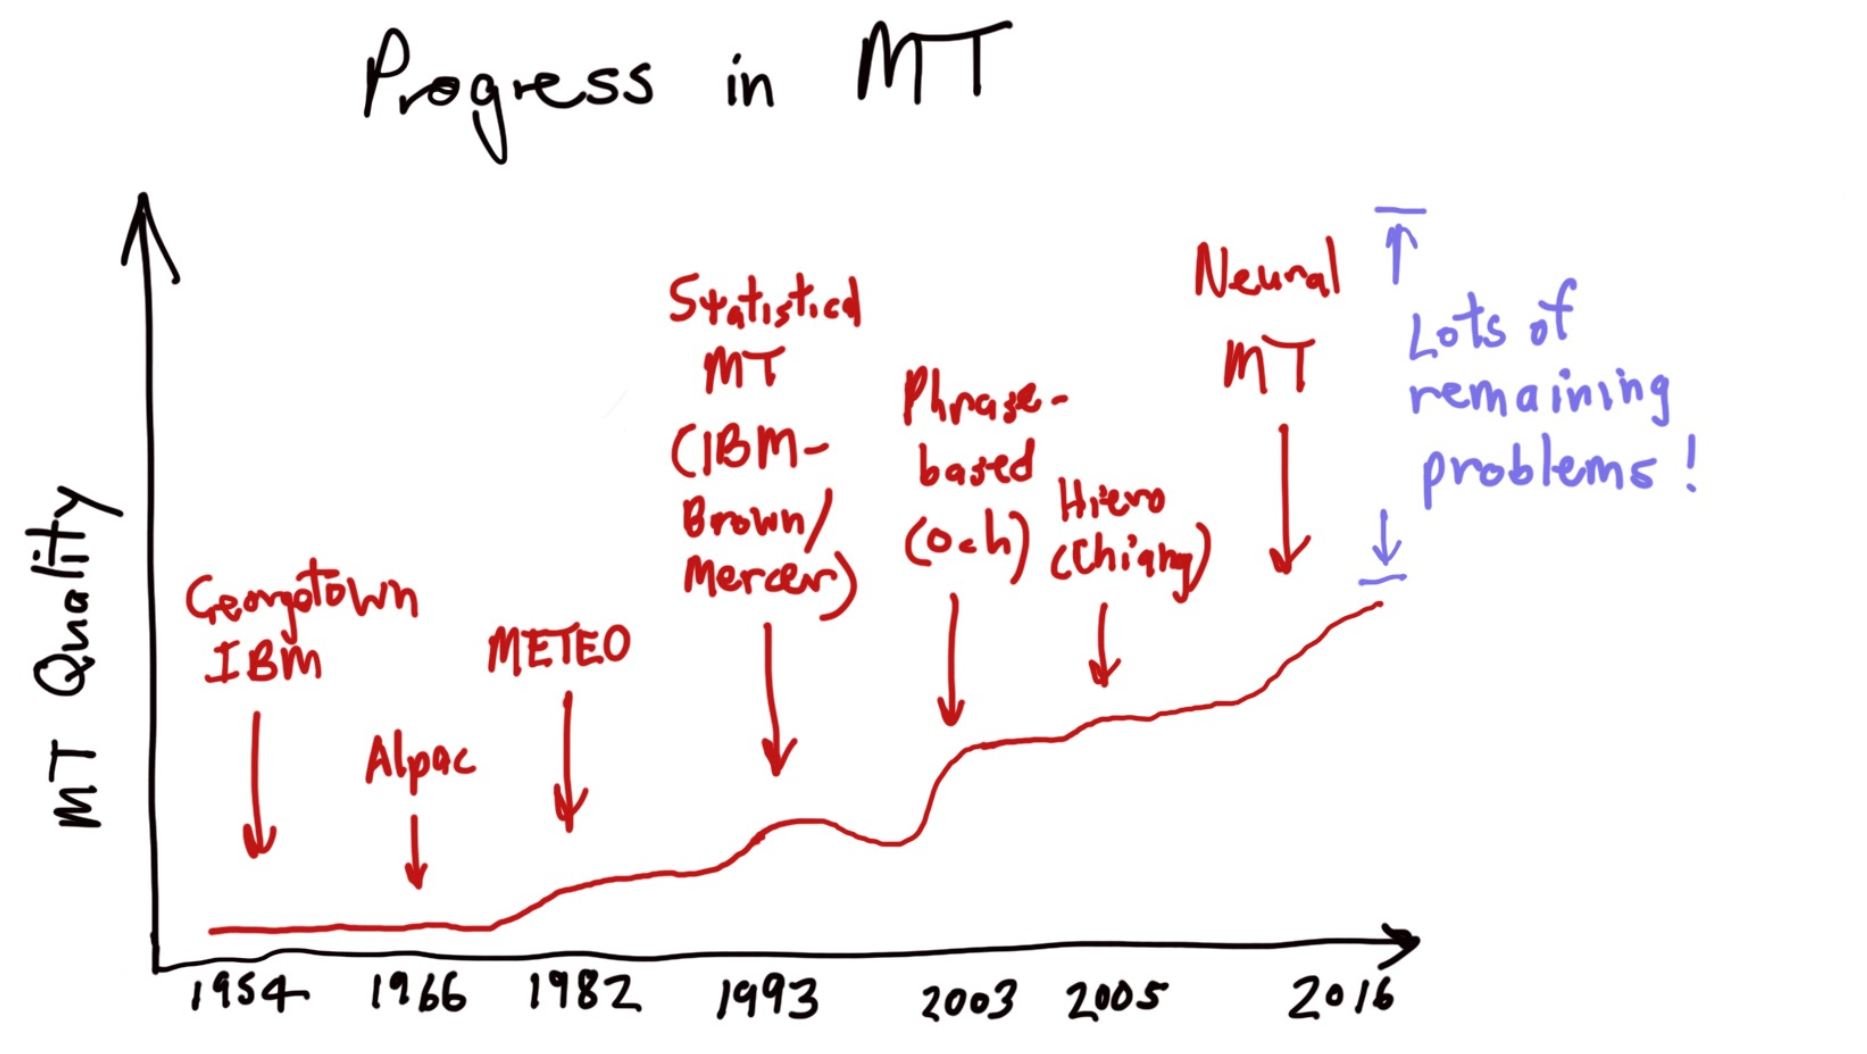
\includegraphics[width=\textwidth, clip=true, trim= 0 0 20 80]{img/MT_progress}
\caption[Machine translation progress]{{\bf Machine translation progress} --
from the 1950s, the starting of modern MT research, until the time of this
thesis, 2016, in which neural MT becomes a dominant approach. Image courtesy of
Christopher D. Manning.
} 
\label{f:mt_progress}
\end{figure}


\section{Machine Translation}
\label{sec:mt}
\begin{figure}
\centering
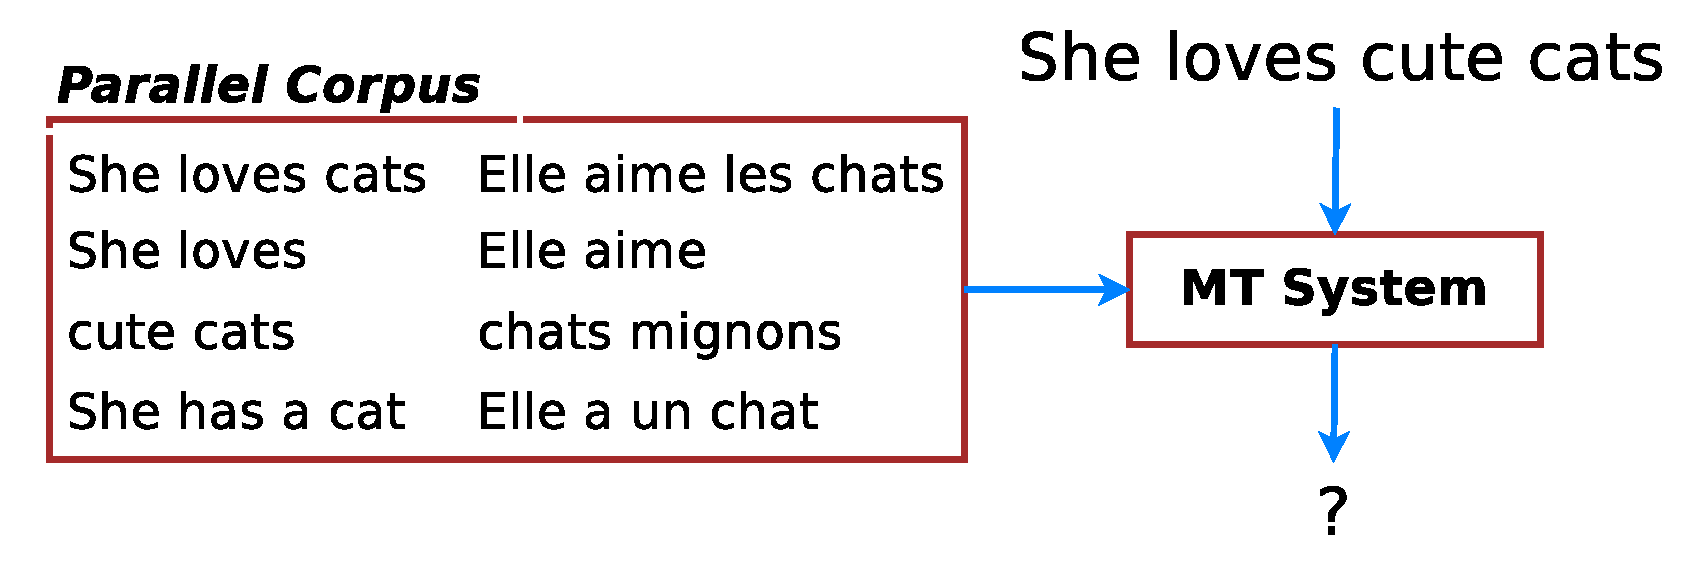
\includegraphics[width=\textwidth, clip=true, trim= 0 0 0 0]{img/mt.eps}
\caption[Corpus-based approaches to machine translation]{{\bf Corpus-based approaches to
machine translation} -- a general setup in which MT systems
are built from parallel corpora of sentence pairs having the same meaning. Once
built, systems are used to translate new unseen
sentences, e.g., \word{She loves cute cats}.}
\label{f:mt}
\end{figure}

Despite much enthusiasm, the beginning period of MT research in the 1950-60s,
was mostly about direct word-for-word replacement based on bilingual
dictionaries.\footnote{There are also proposals for ``interlingual'' and
``transfer'' approaches but these seemed to be too challenging to achieve, not
to mention limitations in hardware at that time \cite{hutchins07}.} An MT winter quickly came
right after the ALPAC report in 1966 pointing out that ``there is no immediate
or predictable prospect of useful machine translation'', which hampered MT
research for over a
decade. Fast-forwarding through the resurgence in the 1980s beginning with
Europe, Japan, and gradually the United States,
modern statistical MT started out with a seminal work by IBM scientists
\cite{Brown:1993:MSM}. The proposed {\it corpus-based} approaches require
minimal linguistic content and only need a {\it parallel} dataset of
sentence pairs which are translations of one
another, to train MT systems.
Such a language-independent setup is illustrated in Figure~\ref{f:mt}. 
In more
detail, instead of hand building bilingual dictionaries which can be costly to
obtain, Brown and colleagues proposed to learn these dictionaries, or {\it
translation models}, probabilistically from parallel corpora. To accomplish
this, they propose a series of 5 algorithms of increasing complexity, often
referred as IBM Models 1-5, to learn {\it word alignment},
a mapping between source and target words in a parallel corpus, as illustrated
in \figref{f:wordalign}. The idea is
simple: the more often two words, e.g., \word{loves} and \word{aime}, occur
together in different sentence pairs, the more likely they are aligned to each
other and have equivalent meanings.

\begin{figure}[tbh!]
\centering
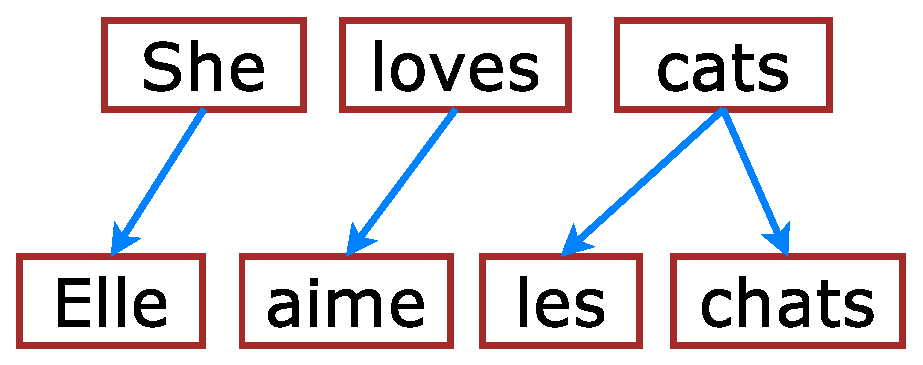
\includegraphics[width=0.35\textwidth, clip=true, trim= 0 0 0
0]{img/wordalign.eps}
\caption[Word-based alignment]{{\bf Word-based alignment} -- example of
an alignment between source and target words. In IBM
alignment models, each target word is aligned to at most one source word.
} 
\label{f:wordalign}
\end{figure}

Once a translation model, i.e., a probabilistic bilingual dictionary, has been
learned, IBM model 1, the simplest and the most na\"{i}ve one among the five proposed
algorithms, translates a new source sentence as follows. First, it decides on
how long the translation is as well as how source words will be mapped to target
words as illustrated in Step 1 of \figref{f:wordmt_algo}. Then,
in Step 2, it produces a translation by selecting for each target position a
word that is the best translation for the aligned source word according to the
bilingual dictionary. Subsequent IBM models build on top of one another and refine the
translation story such as better modeling the reordering structure, i.e., how
word positions differ between source and target languages. I refer the reader to
the original IBM paper or Chapter 25 of \cite{Jurafsky:2009} for more details.

\begin{figure}[tbh!]
\centering
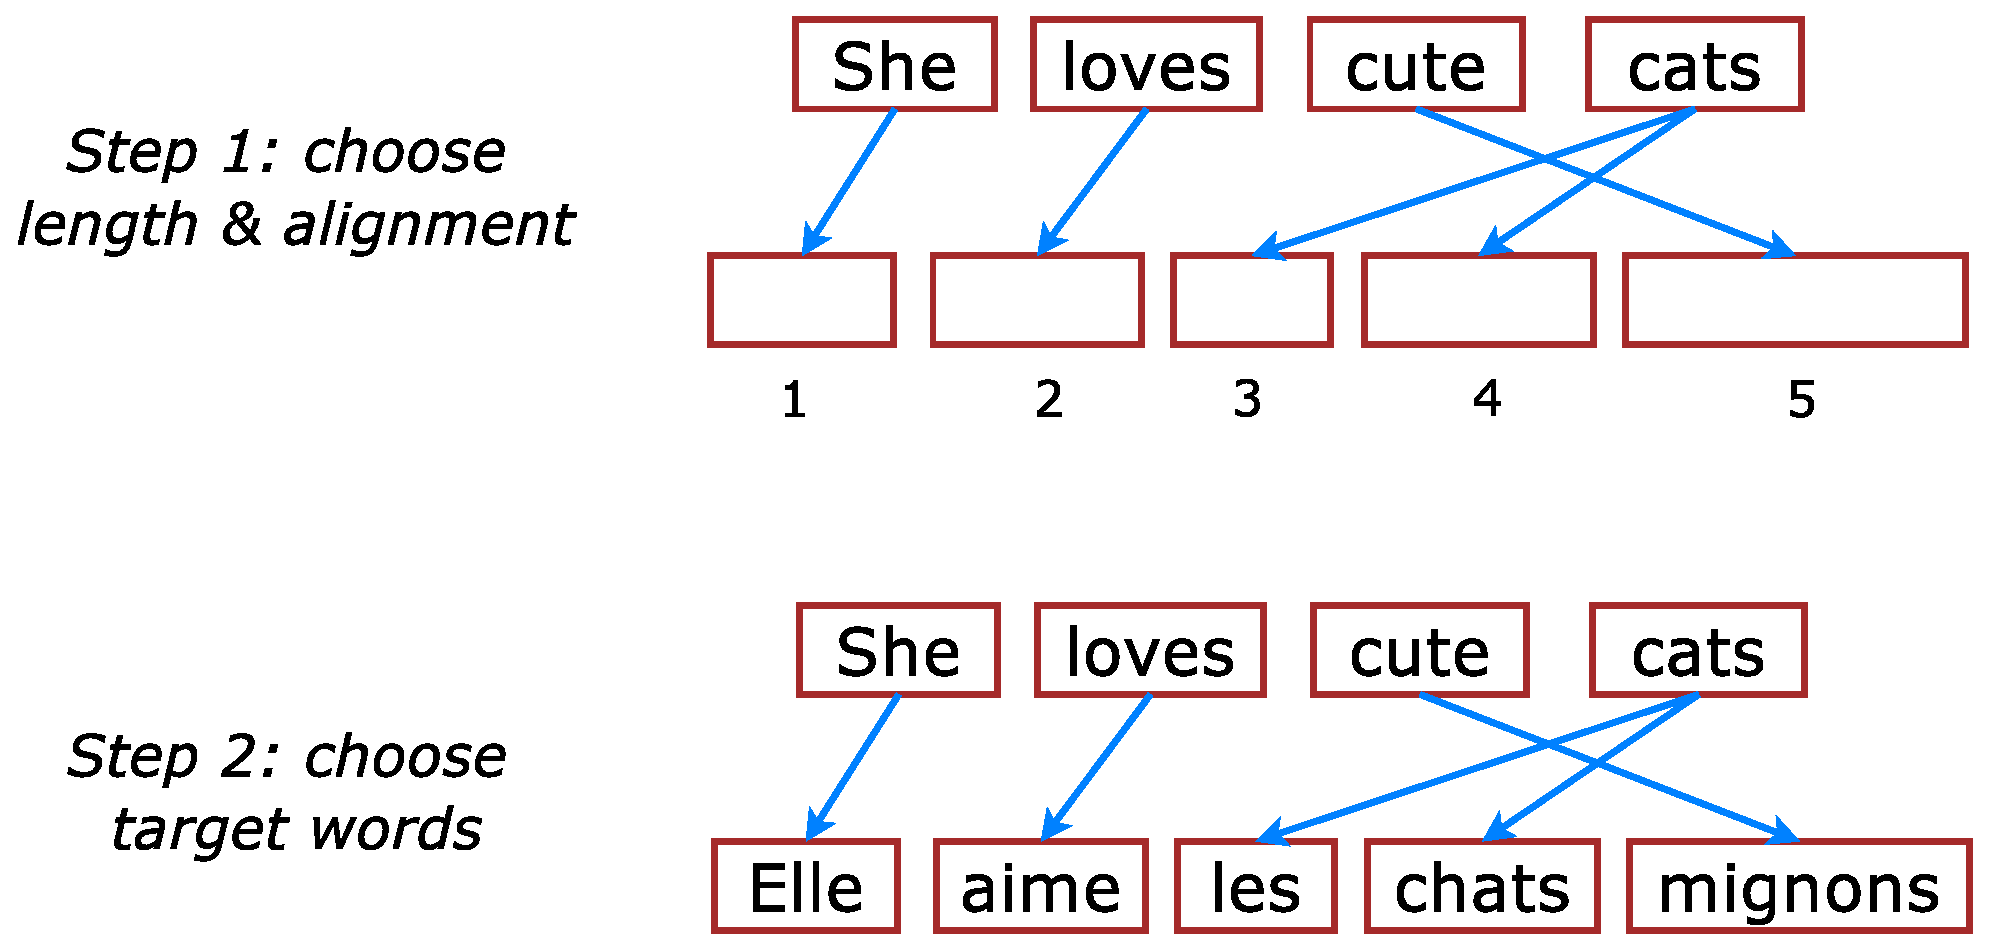
\includegraphics[width=0.8\textwidth, clip=true, trim= 0 0 0
0]{img/wordmt_algo.eps}
\caption[A simple translation story]{{\bf A simple translation story} -- example of the generative story in
IBM Model 1 to produce a target translation given a source sentence and a
learned translation model.
} 
\label{f:wordmt_algo}
\end{figure}

There are, however, two important details that we left out in the above translation story,
the {\it search} process and the {\it language modeling} component. In Step 1,
one might wonder among the exponentially many choices, how do we know what the
right translation length is and how source words should be mapped to target words? The
search procedure informally helps us ``browse'' through a manageable set of
candidates which are likely to include a good translation; whereas, the language
model will help us select the best translation among these candidates. I will
defer details of the search process to later since it depends on the
exact translation model being used. Language modeling, on the other hand, is an
important concept which has been studied earlier in speech recognition
\cite{katz87}. In a nutshell, a language model (LM)
learns from a corpus of monolingual text in the target language and collect
statistics on which sequence of words are likely to go with one another. When
applied to machine translation, an LM will assign high scores for coherent and
natural-sounding translations and low scores for bad ones.
For our example in the above figure, if the model happens to choose a wrong alignment, e.g.,
\word{cute} goes to position 3 while \word{cats} goes to positions 4 and 5, an
LM will alert us with a lower score given to that incorrect translation \word{Elle
aime mignons les chats} compared to the translation \word{Elle aime les chats
mignons} with a correct word ordering structure.\footnote{
For completeness, translation and
language models are integrated together in an MT system through the {\it
Bayesian noisy channel} framework as follows:
\begin{align}
\label{e:noisy}
\hat{t} &= \argmax_t P(t|s) \approx \argmax_t P(s|t) P(t)
\end{align}
Here, we have a source sentence $s$ in which we ask our {\it decoder}, an
algorithm that implements the aforementioned search process, to find the best
translation, the $\argmax$ part. $P(s|t)$ represents the {\it translation} model, the
faithfulness of the translation in terms of meaning preservation between the source and the
target sentences; whereas $P(t)$
represents the {\it language} model, the fluency of the translated text.
}

While the IBM work had a huge impact on the field of statistical MT, researchers
quickly realized that word-based MT is insufficient as words
require context to properly translate, e.g., \word{bank} has two totally different
meanings when preceded by \word{financial} and \word{river}. As a result,
{\it phrase-based models}, \cite{Marcu:2002,Koehn:2003:SMT}, inter alia, became the de facto
standard in MT research and are still the dominant approach in existing
commercial systems until recently.\footnote{However, the landscape is changing rapidly! As I am preparing this dissertation, there have been recent announcements from Google Translate \cite{gnmt16} in September 2016 and SYSTRAN \cite{systran16} in October 2016 on using Neural Machine Translation for their production systems.} Much credit went to Och's
work on {\it alignment templates}, starting with his thesis in 1998 and later in
\cite{och03,och04}. The idea of alignment templates is to enable phrase-based MT
by first symmetrizing\footnote{Symmetrization is achieved by training IBM models
in both directions, source to target and vice versa, then intersecting the
alignments. There are subsequent techniques that jointly train alignments in
both directions such as \cite{liang06alignment}.} the alignment to obtain many-to-many correspondences
between source and target words; in contrast, the original IBM models only produce
one-to-many alignments. From the symmetrized alignment, several heuristics have
been proposed to extract phrase pairs; the general idea is that phrase
pairs need to be ``consistent'' with their alignments: each word in a phrase
should not be aligned to a word outside of the other phrase. These pairs are stored
in what called a {\it phrase table} together with various scores to evaluate
phrase pairs in different aspects, e.g., how equivalent the meaning is, how good
the alignment is, etc. \figref{f:phrase_mt} gives an example of how a
phrase-based system translates.

\begin{figure}[tbh!]
\centering
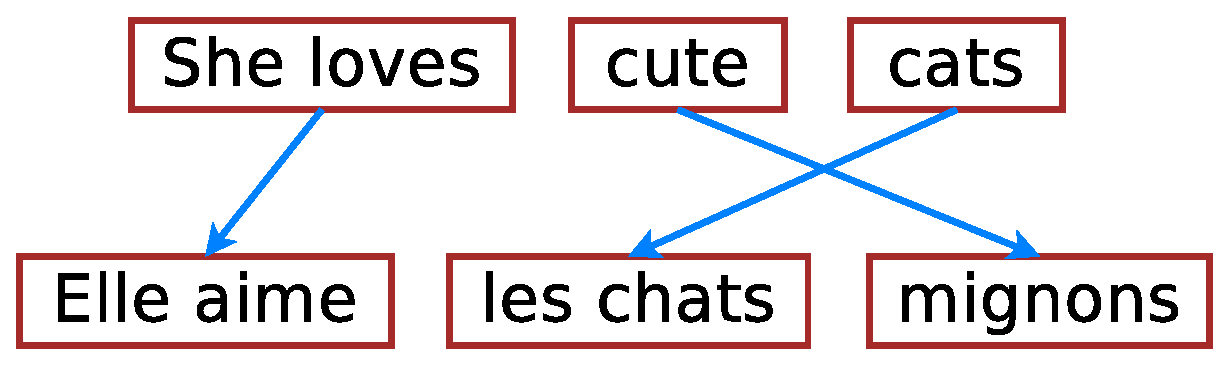
\includegraphics[width=0.45\textwidth, clip=true, trim= 0 0 0
0]{img/phrasemt.eps}
\caption[Phrase-based machine translation]{{\bf Phrase-based machine translation} (MT) -- example of how phrase-based
MT systems translate a source sentence \word{She loves cute cats} into a target sentence
\word{Elle aime les chats mignons}: sentences are split into chunks and phrases
are translated.
} 
\label{f:phrase_mt}
\end{figure}

%% log-linear models %%
State-of-the-art MT systems, in fact, contain more components than just the two
basic translation and language models. There are many knowledge
sources that can be useful to the translation task, e.g., language model,
translation model, reversed translation model, reordering
model\footnote{Reordering models learn the patterns of how words move across source
and target sentences and are trained based on the word alignment.},
length/unknown penalties\footnote{To produce translations of appropriate lengths
and with a reasonable amount of unknown words, e.g., unseen names and numbers
at test time.}, etc. To incorporate all of
these features, modern MT systems use a popular framework in natural language
processing, called the {\it maximum-entropy} or
{\it log-linear} model \cite{berger96,och02}, which has as its special case the
Bayesian noisy channel model that we briefly mentioned in \eq{e:noisy}.

Training log-linear MT models can be done using the standard {\it maximum
likelihood estimation} approach. However, in practice, these models are learned
by directly optimizing translation quality metrics such as BLEU
\cite{Papineni02bleu} in a technique known as {\it minimum error rate training}
or {\it MERT} \cite{och03mert}. Here, BLEU is an inexpensive automatic way of
evaluating the translation quality; the idea is to count words and phrases that
overlap between machine and human outputs. Despite many criticisms, BLEU is
still the most widely used evaluation metric up until now thanks to its
simplicity. 

Lastly, there has also been effort in
adding {\it syntax} to machine translation through tree-based models such as work by
\newcite{wu97,yamada01,chiang05}, inter alia. As illustrated in
\figref{f:mt_progress}, these approaches do provide gains
for several language pairs, mostly those that are significantly different in terms
of sentence structures such as Chinese and English. However,
the gains are often modest compared to the added complexity of tree-based models
such as requirements to have good parsers and syntactic annotations.

For more information on evaluation metrics, tree-based models, and other
topics in statistical machine translation, we refer the audience to an 
excellent book by \newcite{koehn10smt}.

\section{Neural Machine Translation}
While statistical machine translation (SMT) has been successfully deployed in many
commercial systems, it does not work very well and suffers from the following
two major drawbacks.
First, translation decisions are {\it locally determined} as we translate
phrase-by-phrase and long-distance dependencies are often ignored. 
More problematically, the entire MT pipeline is becoming increasingly {\it
complex} as more and more features are added to the log-linear framework
such as in recent MT systems \cite{galley08,chiang09,green13}. Many different
components need to be tuned
separately, e.g., translation models, language models, reordering models, etc.,
which makes it difficult to combine them together and to innovate. As a result,
the translation quality has saturated for SMT and big changes to the
existing framework were in dire need.

Neural Machine Translation (NMT) is a new approach 
that addresses the aforementioned problems. First, NMT is a {\it single big neural
network} (with millions of artificial neurons) that is designed to model the
entire MT process 
\cite{kal13,sutskever14,cho14}. NMT requires {\it minimal domain knowledge}, just a
parallel corpus of source and target sentence pairs, similar to SMT, but with far
less preprocessing steps before a translation model can be built.
The most appealing feature of NMT is that it can be
trained {\it end-to-end} directly from the learning objective; hence, eliminating the
problem of having to learn multiple components in SMT systems. 

Unlike those intricate decoders (the search procedure we mentioned earlier) in popular SMT packages
\cite{koehn2007moses,chiang07hiero,dyer10cdec,cer10phrasal}, the translation
story of NMT is conceptually simple.
NMT translates as follows: an {\it encoder} reads through the given source
sentence to build a ``thought''
vector\footnote{This term was coined by Geoffrey Hinton in this article
\url{https://www.theguardian.com/science/2015/may/21/google-a-step-closer-to-developing-machines-with-human-like-intelligence}.},
a sequence of numbers that represents the sentence meaning; a {\it
decoder}, then, processes the sentence vector to emit a translation, as
illustrated in Figure~\ref{f:nmt}. 
This is often referred to as the encoder-decoder
architecture.\footnote{\newcite{allen87,chrisman91} wrote the very first papers
on %\newcite{forcada97} 
encoder-decoder models for translation!} In this manner, NMT addresses the
local translation problem in SMT; it does not do phrase-by-phrase translation.
Instead, NMT gathers information from the entire source sentence before translating; as a result,
it can capture {\it long-range dependencies} in languages, e.g., gender
agreements; structural orderings of subject, verb, and object; etc.
\begin{figure}[tbh!]
\centering
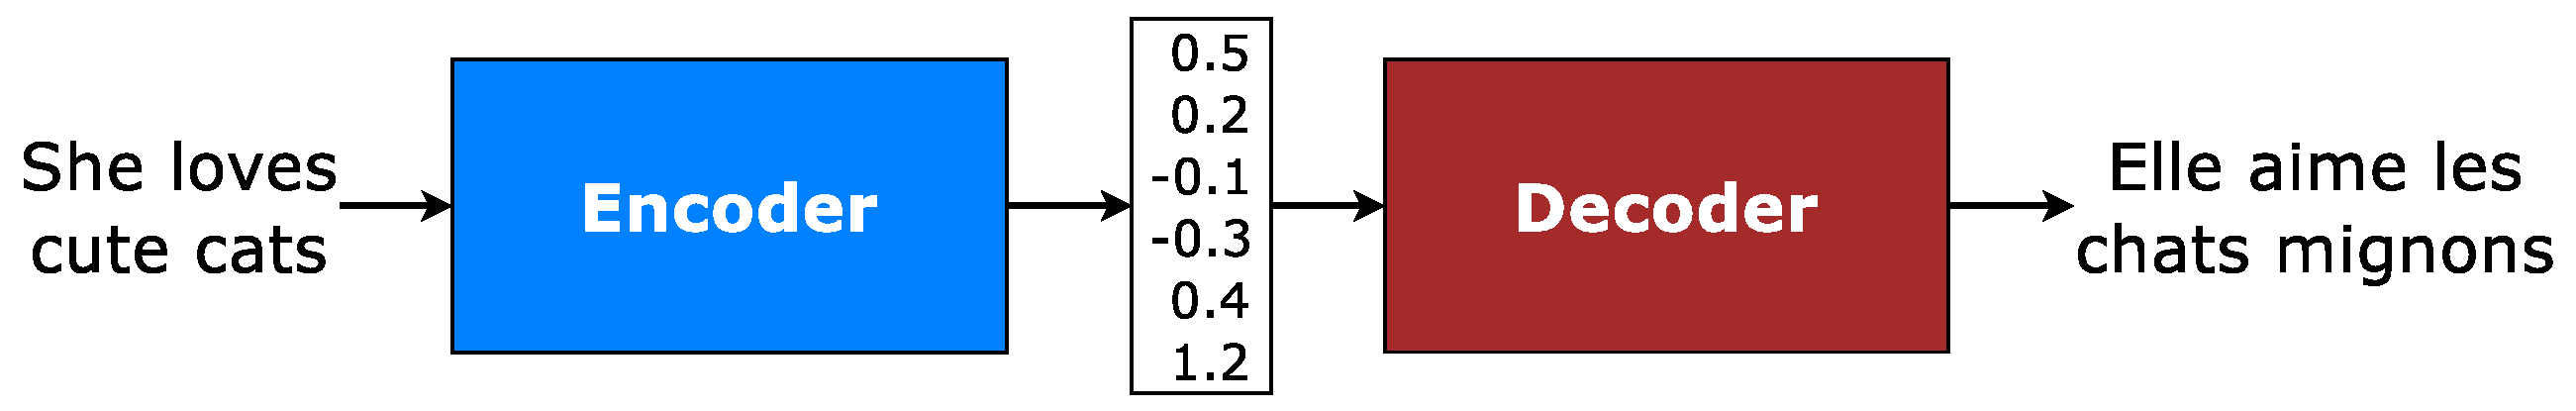
\includegraphics[width=\textwidth, clip=true, trim= 0 0 0 0]{img/encdec}
\caption[Encoder-decoder architecture]{{\bf Encoder-decoder architecture} --
example of the general approach for NMT. An {\it encoder} converts a source sentence
into a meaning vector which is passed through a {\it decoder} to produce a translation.
} 
\label{f:encdec}
\end{figure}

A realization of NMT is to use a powerful model for sequential data, namely recurrent
neural network (RNN), for both the encoder and decoder \cite{sutskever14,cho14}.
Interested readers can find details about RNNs in
\secref{sec:rnn}; in a nutshell, RNNs allow us to build representations for
variable-length input -- in our case, sentences -- using a dynamic memory
structure. In \figref{f:nmt}, deep RNNs with two stacking layers are used to build
a sequence-based NMT: an encoder first constructs a representation for a source
sequence; a decoder, then, generates a target sequence,
one symbol at a time until a special end-of-sequence symbol is produced.

Sequence-based NMT has several advantages.
First, NMT beam-search decoders that generate words from left to right can be
easily implemented, unlike the highly complex beam-search decoders in SMT
\cite{Koehn:2003:SMT}. More importantly, the use of
RNNs in NMT allows for {\it better generalization} to very long
sequences while not having to  explicitly store any gigantic
phrase tables or language models as in the case of SMT.
As sequence-based NMT is currently the de facto approach, we will use NMT to
generally refer to sequence-based NMT
throughout this thesis unless otherwise stated.

\begin{figure}[tbh!]
\centering
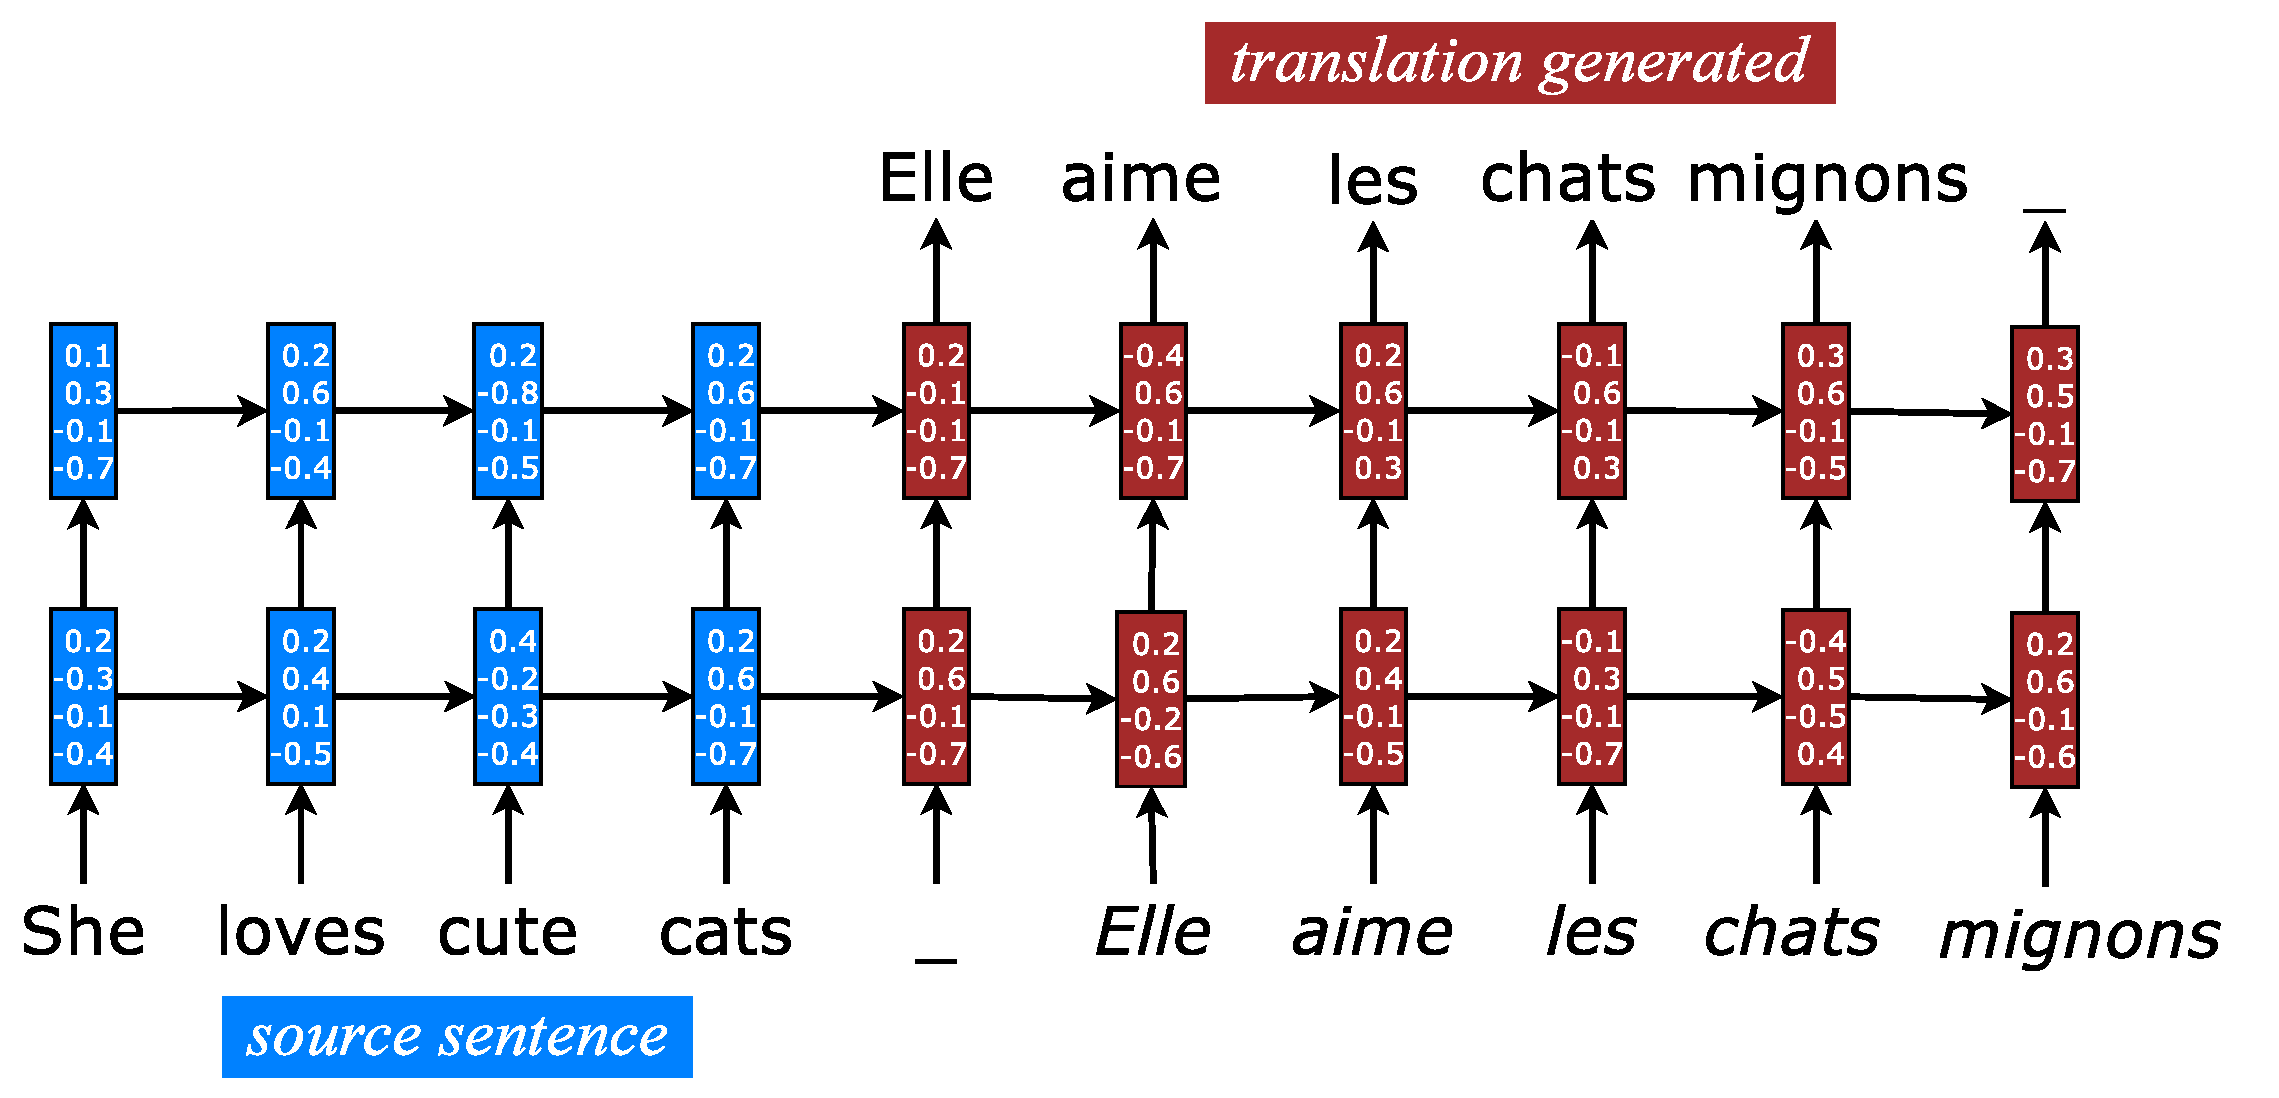
\includegraphics[width=\textwidth, clip=true, trim= 0 0 0
0]{img/nmt_intro}
\caption[Sequence Models for NMT]{{\bf Sequence Models for NMT} -- example of a
deep recurrent architecture for translating a source sentence \word{She loves
cute cats} into a target sentence \word{Elle aime les chats mignons}. On the
decoder side, {\it words} generated from previous timesteps are used as inputs for the
next ones. Here, \word{\texttt{\_}} marks the end of a sentence.
} 
\label{f:nmt}
\end{figure}

\section{Thesis Outline}
Despite all the aforementioned advantages and potentials, the early NMT architecture
\cite{sutskever14,cho14} still has many drawbacks. In this thesis, I will
highlight three problems pertaining to the existing NMT model, namely the
{\it vocabulary coverage}, the {\it memory constraint}, and the {\it
language complexity} issues. Each chapter is devoted to solving one of these
problems. In each chapter, I will describe how I have pushed the limits of NMT, making it
applicable to a wide variety of languages with state-of-the-art performance such as
English-French \cite{luong15}, English-German \cite{luong15attn,luong15iwslt},
English-Vietnamese \cite{luong15iwslt}, and
English-Czech \cite{luong16}. Towards the {\it future} of
NMT, I answer two questions: (1) whether we can improve translation by jointly
learning from a wide variety of sequence-to-sequence tasks such as parsing,
image caption generation, and auto-encoders or skip-thought vectors
\cite{luong16iclr}; and (2)
whether we can compress NMT for mobile devices \cite{see16}.
In brief, this thesis is organized as follows. I start off by providing background knowledge on RNN and NMT
in Chapter~\ref{c:background}. 
The aforementioned three problems and approaches to the future of NMT are detailed in
Chapters~\ref{c:copy},~\ref{c:attention},~\ref{c:hybrid}, and~\ref{c:future}
respectively, which we will go through one by one next.
%My contributions are detailed in:
%Chapter~\ref{c:copy} on the rare word problem, Chapter~\ref{c:attention} on the
%sentence length problem, Chapter~\ref{c:hybrid} on the language complexity
%problem, and Chapter~\ref{c:future} on the future of NMT.
Chapter~\ref{c:conclude} wraps up and discusses remaining challenges in NMT research.

\subsubsection*{Copy Mechanisms} 
%\paragraph{Copy Mechanisms} 
A significant weakness in the first NMT 
systems is their inability to correctly translate very rare words:  
end-to-end NMTs tend to have relatively small vocabularies with a single
\unk{} symbol that represents every possible out-of-vocabulary (OOV) word. In
Chapter~\ref{c:copy}, I propose simple and effective techniques to address this
{\it vocabulary size} problem through teaching NMT to ``copy'' words from source to
target. Specifically, I train an NMT system on data that is augmented by the output of a word 
alignment algorithm, allowing the NMT system to emit, for each OOV word
in the target sentence, the position of its corresponding word in the source sentence.
This information is later utilized in a
post-processing step that translates every OOV word using a dictionary. My 
experiments on the WMT'14 English to French translation task show that this 
method provides a substantial improvement of up to 2.8 BLEU points over an
equivalent NMT system that does not use this technique. 
With 37.5 BLEU points, this NMT system is the first to surpass 
the best result achieved on a WMT'14 contest task. 
{\it This chapter is based
on the following paper \cite{luong15} in which I, Ilya Sutskever, and Quoc Le
share the first co-authorship.}

\subsubsection{Attention Mechanisms} 
%\paragraph{Attention Mechanisms} 
While NMT can translate well for short- and medium-length sentences, it 
has a hard time dealing with long sentences.
An attentional mechanism was proposed by \newcite{bog15} to address that {\it
sentence length} problem by
selectively focusing on parts of the source sentence during translation. However,
there has been little work exploring useful architectures for attention-based
NMT. Chapter~\ref{c:attention} examines two simple and effective classes of attentional
mechanism: a {\it global} approach which always attends to all source words and
a {\it local} one that only looks at a subset of source words at a time. 
I demonstrate the effectiveness of both approaches on the WMT translation
tasks between English and German in both directions. With local
attention, I achieve a significant gain of 5.0 BLEU points over
non-attentional systems that 
already incorporate known techniques such as dropout. My ensemble 
model using different attention architectures yields a new
state-of-the-art result in the WMT'15 English to German
translation task with 25.9 BLEU points, an improvement of 1.0 BLEU points over the existing
best system backed by NMT and an $n$-gram reranker. 
{\it This chapter is based
on the paper \cite{luong15attn}.}\footnote{ 
Besides, I also have a follow-up paper \cite{luong15iwslt} on applying these attention-based models to
the {\it transfer learning} and {\it low-resource} settings for TED talk translation, which obtains
state-of-the-art performance for English-German and English-Vietnamese \cite{iwslt15}.}

\subsubsection{Hybrid Models} 
Nearly all previous NMT work has used quite restricted
vocabularies, perhaps with a subsequent method to patch in unknown words such as
the copy mechanisms mentioned earlier. While effective, the copy mechanisms cannot deal with all the
complexity of human languages such as rich morphology, neologisms, and informal
spellings.
Chapter~\ref{c:hybrid} presents a novel word-character solution to that {\it
language complexity} problem towards achieving
open vocabulary NMT.
I build hybrid systems that translate mostly at the {\it word}
level and consult {\it character} components for rare words. 
My character-level recurrent neural networks compute source
word representations and recover unknown target words when needed.
The twofold advantage of such a hybrid approach is that it is much faster and easier to
train than character-based ones; at the same time, it never produces unknown words as in the case of word-based models. 
On the WMT'15 English to Czech translation task, 
this hybrid approach offers an addition boost of +$2.1{-}11.4$ BLEU points over models 
that already handle unknown words. 
My best system achieves a new state-of-the-art result with
$20.7$ BLEU score.
I demonstrate that my character models can successfully learn to not only generate well-formed words for Czech, a
highly-inflected language with a very complex vocabulary, but also build correct
representations for English source words.
{\it This chapter is based on the following paper \cite{luong16}}, which takes inspirations from my earlier work \cite{luong13} and \cite{li15}.

\subsubsection{The Future of NMT} 
Chapter~\ref{c:future} answers the two aforementioned questions
for the future of NMT: whether we can utilize other tasks to improve
translation and whether we can compress NMT models. 
The former question is important because of the fact that the first NMT systems only
utilize parallel corpora despite an abundant amount of available data from
monolingual and multi-lingual corpora as well as data from related tasks. The
latter question is motivated by the indispensable role of mobile devices in 
society nowadays\footnote{In 2014, the number of mobile devices is more than the number
of people in the world \cite{mobiledevices}.} 
and the fact that state-of-the-art NMT models are beyond the storage capacity of
existing mobile gadgets.

For the first question, 
I examine three multi-task learning (MTL) settings for sequence to sequence
models:
(a) the {\it one-to-many} setting -- where the encoder is shared
between several tasks such as machine translation and
syntactic parsing, (b) the {\it many-to-one} setting -- useful when only the
decoder can be shared, as in the case of 
translation and image caption generation, and (c) the {\it
  many-to-many} setting -- where multiple encoders and decoders are
shared, which is the case with unsupervised objectives
and translation.  My results show that training on a small amount of parsing and
image caption data can improve the translation quality between English and
German by up to $1.5$ BLEU
points over strong single-task baselines on the WMT benchmarks. Rather
surprisingly,
I have established a new {\it
state-of-the-art} result in constituent parsing with 93.0 F$_1$ by utilizing
translation data. Lastly, I reveal interesting properties of the two unsupervised learning
objectives, autoencoder and skip-thought, in the MTL context: an autoencoder helps less in terms of
perplexity but more on BLEU scores compared to skip-thought.
{\it This section is based on the following paper \cite{luong16iclr}.}

For the second question, I examine three simple magnitude-based pruning schemes to compress NMT models, namely {\it class-blind}, {\it class-uniform}, and {\it class-distribution}, which differ in terms of how pruning thresholds are computed for the different classes of weights in the NMT architecture.
I demonstrate the efficacy of weight pruning as a compression technique for a state-of-the-art NMT system. 
I show that an NMT model with over 200 million parameters can be pruned by 40\% with very little performance loss as measured on the WMT'14 English-German translation task. 
This sheds light on the distribution of redundancy in the NMT architecture.
My main result is that with {\it retraining}, I can recover and even surpass the original performance with an 80\%-pruned model. 
{\it This section is based on the following paper \cite{see16} in which
Abigail See and I share the first co-authorship.}

\subsubsection{Wrap-up} 
In summary, this thesis has touched on a variety of aspects in which NMT can be
significantly improved. My hope is to convince the reader 
at the end of this thesis that NMT models have successfully taken over the role
of SMT models and will continue to be the de facto standard for several years
to come. Still, there are many challenging and rewarding problems to be explored
which I will summarize in the conclusion chapter. {\it The material is based on an
NMT tutorial given by me, Kyunghuyn Cho, and Christopher D. Manning at
ACL'2016}.\footnote{The tutorial website is
at \url{https://sites.google.com/site/acl16nmt/}.}

\begin{sloppypar}
All code, data, and models used in this thesis can be found at \url{http://nlp.stanford.edu/projects/nmt}.
\end{sloppypar}



\chapter{Background}
\label{c:background}
\epigraph{For neural machine translation, it all started from language
modeling.}{Thang Luong.}

Language modeling plays an
indispensable role in ensuring that machine translation systems produce fluent target
sentences and has always been an active area of research.
Despite much effort in improving traditional \ngram{} language models
\cite{rosenfeld2000,srilm,teh2006,irstlm,kenlm,pauls2011,heafield13},
traditional LMs inherently can only handle short
contexts of a few words. Approaches to building \nlmtext{} (\nlms) using
feed-forward networks such as those initiated by \newcite{Bengio2003} and
enhanced by others \cite{Morin2005,Bengio08,MnihHinton2009,MnihTeh2012} have %,Mnih2007
addressed that drawback to model longer contexts.
% worked great compared to traditional \ngram{} language models. 
Still, \nlms{} can only capture fixed-length contexts and is
incapable of handling variable-length sequences, which is the case for sentences.
Recurrent neural networks (RNNs) come in handy as a powerful and expressive
architecture to handle sequential data and have successfully been applied to the
language modeling task \cite{MikolovKBCK10,MikolovKBCK11,mikolovLM}.
By viewing RNNs as generative models \cite{Sutskever11} that can produce texts 
and by pushing another step towards conditioning RNNs on source sentences, recent works
\cite{kal13,sutskever14,cho14} have started a new line of resesarch in machine translation, namely Neural
Machine Translation (NMT). NMT is technically a source-conditioned \nlm{} that
can be trained end-to-end.

%Early success of feed-forward \nlms{} has led to widespread adoption of \nlms{}
%as an additional component in the machine translation pipeline
%such as \cite{schwenk07,vaswani13decode,luong15nlm}, inter alia.
%\cite{Schwenk12continuous,Son:2012:CST,Auli13,devlin14}

%An important part in the machine translation pipeline is the ability to model language
%coherence at the target side. 
%As such, a significant amount of effort in
%improving MT has centered around enhancing language modeling -- more specifically, the need to capture long-range
%dependencies better. We start out with efforts to scale up traditional \ngram{} language models 

In this chapter, we provide background knowledge on two main topics, RNN and NMT.
We first go through the basics of RNNs, explaining how they can be used to model sentences. 
Then, we delve into details of one particular type of RNNs, the Long Short-term Memory, that makes training RNNs easier.
Given RNNs as a building block, we discuss NMT together with tips and tricks for better training and testing NMT.

\section{Recurrent Neural Network}
\label{sec:rnn}
Recurrent Neural Network (RNNs) \cite{elman90} are models that help understand
the temporal aspect as well as build up representations for sequential data
using a dynamic memory structure. At the surface form, an RNN takes as input a sequence of vectors $\x{1},
\x{2}, \ldots, \x{n}$ and processes them one by one. For each
new input $\x{i}$, an RNN updates its memory to produce a hidden state
$\hid{i}$ which one can think of as a representation for the partial sequence
$\x{\overline{1,i}}$. %$\x{1},\ldots, \x{i}$. 
The beauty of RNNs lies in the fact that it can
capture the dynamics of an arbitrarily long sequence without having to increase its modeling
capacity unlike the case of feedforward network which can only model
relationship within a fixed-length sequence. The key secret sauce is in the
recurrence formula of an RNN that defines how its hidden state is updated. At
its simplest form, a ``vanilla'' RNN defines its recurrence function as:
\begin{align}
\hid{t} &= f\paren{\x{t}, \hid{t-1}} \label{e:abstract_rnn}
\end{align}
In the above formula, $f$ is an abstract function that computes a new hidden state given the current input $\x{t}$ and the
previous hidden state $\hid{t-1}$. The starting state $\hid{0}$ is often set to
$\bm{0}$ though it can take any value as we will see later in the context
of NMT decoders. A popular choice of $f$ is provided below with $\sigma$ being a
non-linear function such as $\sigmoid$ or $\tanh$.\footnote{There could also be
an optional bias term in \eq{e:vanilla_rnn}.}
\begin{align}
%\z{t} &= \W{xh}\x{t} + \W{hh}\hid{t-1} \label{e:vanilla_rnn} \\
\hid{t} &= \sigma(\W{xh}\x{t} + \W{hh}\hid{t-1} \label{e:vanilla_rnn}) %\z{t})
\end{align}

At each timestep $t$, an RNN can (optionally) emit an output symbol
$y_t$ which can either be discrete or real-valued. For the discrete scenario,
which is often the case for languages, a probability distribution $\bm{p}$ over a 
set of output classes $Y$ is derived as
follows\footnote{For the real-valued case, we refer readers to mixture density
models \cite{bishop94} which have been applied to RNN training, e.g., for
hand-writing synthesis \cite{graves13c}.}:
\begin{align}
\s{t} &= \W{hy}\hid{t} \label{e:score} \\
\prob{t} &= \softmax(\s{t}) \label{e:prob}
\end{align}
Here, we introduce a new set of weights $\W{hy} \inR{|Y| \times d}$, with $d$ being the dimension of the RNN hidden
state, to compute a score vector $\s{t}$, or {\it logits}, over
different individual classes. Often, with a large output set $Y$, the
matrix-vector multiplication in \eq{e:score} is a major computational
bottleneck in RNNs, which results in several challenges for neural language modeling
and machine translation that we will address in later chapters. 
The $\softmax$ function transforms the score
vector $\s{t}$ into a probability vector $\prob{t}$, which is defined for each specific
element $y \in Y$ as below.
For convenience, we overload our notations to use $\prob{t}(y)$ and $\s{t}(y)$ to refer to entries in
the vectors $\prob{t}$ and $\s{t}$ that correspond to $y$.
\begin{align}
\prob{t}(y) = \frac{\e^{\s{t}(y)}}{\sum_{y' \in Y} \e^{\s{t}(y')}}
\label{e:softmax}
\end{align}

With the above formulas, we have completely defined the RNN weight set $\thetav$
%=\!\{\W{xh}, \W{hh}, \W{hy}\}$, 
which consists of {\it input} connections $\W{xh}$, {\it
recurrent} connections $\W{hh}$, and {\it output}
connections $\W{hy}$. These weights are shared across
timesteps as illustrated in Figure~\ref{f:rnn} \error{Draw a picture on
general RNNs}, which enables
RNNs to handle arbitrarily long sequences.

\begin{figure}[tbh!]
\centering
%\psgrid
\rput(7.1,2.6){{\color{lightblue} $\MB{W_{hh}}$}}
\rput(8.6,1.0){{\color{lightgreen} $\MB{W_{xh}}$}}
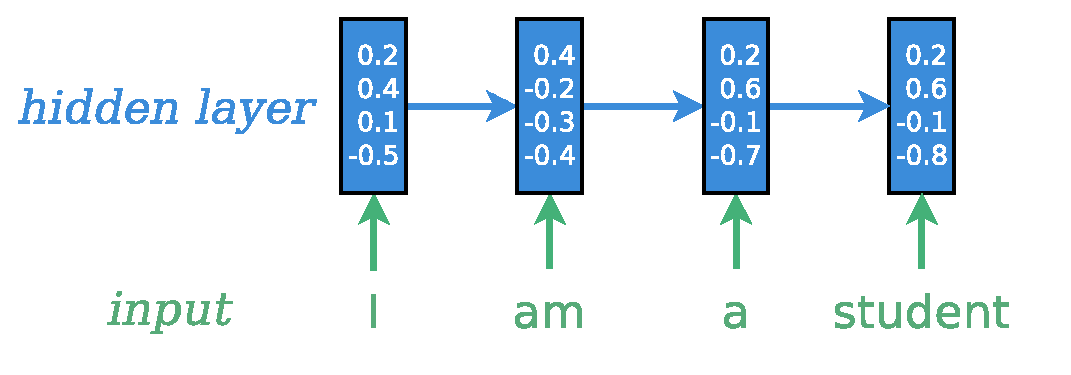
\includegraphics[width=0.6\textwidth, clip=true, trim= 0 0 0 0]{img/rnn.eps} % , angle=-90
\caption[Recurrent neural networks]{{\bf Recurrent neural networks} -- example of a recurrent
neural network that processes a sequence of input words \word{I am a student} to
build up hidden representations as input symbols are consumed. The recurrent
$\MB{W_{hh}}$ and feed-forward $\MB{W_{xh}}$ weights are shared across
timesteps.
} 
\label{f:rnn}
\end{figure}

Next, we discuss the training and testing phases of RNNs from a slightly more
focused angle, the language learning aspect. For more details on RNNs, we refer readers to the following resources
\cite{sutskever12,mikolov12,karpathy15rnn}.

\subsection{Recurrent Language Models}
\label{subsec:rlm}
To apply RNNs to sentences in languages, or generally sequences of discrete symbols, one can
consider one-hot representations $\x{i} \inR{|V|}$, with $V$ being the
vocabulary considered. However, for a large
vocabulary $V$, such a representation choice is problematic as it results in
a large weight matrix $\W{xh}$ and there is no notion of similarity between
words. In practice, low-dimensional dense representations for words, or {\it
word embeddings}, are often used to address these problems. Specifically, an
embedding matrix
$\W{e} \inR{d_e \times |V|}$ is looked up for each word $x_i$ to retrieve a
representation $\x{i} \inR{d_e}$. As a result, a simple RNN applied to language
modeling will generally have $\theta = \{\W{xh}, \W{hh}, \W{hy}, \W{e}\}$ as its
weights as illustrated in Figure~\ref{f:rlm} \error{Draw an RNN with
embedding}.

\begin{figure}[tbh!]
\centering
%\psgrid
\rput(7.1,2.6){{\color{lightblue} $\MB{W_{hh}}$}}
\rput(8.6,1.0){{\color{lightgreen} $\MB{W_{xh}}$}}
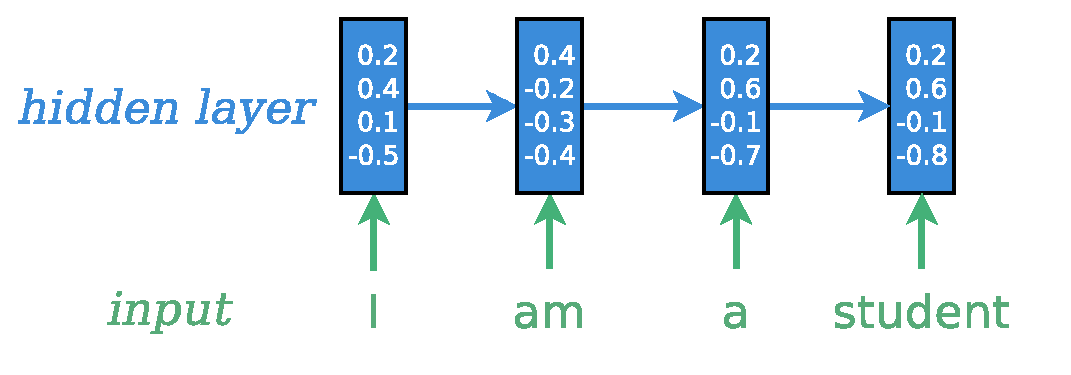
\includegraphics[width=0.6\textwidth, clip=true, trim= 0 0 0 0]{img/rnn.eps} % , angle=-90
\caption[Recurrent language models]{{\bf Recurrent language models} -- example of a recurrent
neural network that processes a sequence of input words \word{I am a student} to
build up hidden representations as input symbols are consumed. The recurrent
$\MB{W_{hh}}$ and feed-forward $\MB{W_{xh}}$ weights are shared across
timesteps.
} 
\label{f:rlm}
\end{figure}

In language modeling (LM), the task is to specify a probability distribution over
sequences of symbols (often, words) so that one can judge if a sequence of
words is more likely or ``fluent'' than another. To accomplish that, an LM decomposes the
probability of a word sequence $y = y_1, \ldots,
y_m$ as:
\begin{align}
p(y) = \prod_{i=1}^m p(y_i | y_{<i}) %\yrange{1}{i-1})
\end{align}
In the above formula, each of the
individual term $p(y_i | y_{<i})$ is the conditional probability of the current
word $y_i$ given previous words $y_{<i}$, also referred as the {\it
context} or the {\it history}. To model these conditional probabilities, traditional \ngram{}
as well as feedforward-based neural language models have to resort to the
Markovian assumption to model only a fixed window of context, i.e., $p(y_i |
y_{i-n+1}, \ldots, y_{i-1})$. An RNN-based language model naturally lends itself to model the full
history as we shall see now.

An RNN-based language model (RNNLM) is a special case of RNNs in which: (a) the input and output
are sequences of discrete words, (b) the output sequence ends %$y=\{y_1, \ldots, y_n$, \eos$\}$ 
with a special symbol \eos{} that marks the boundary, e.g., $y=\{$ ``I'', ``am'', ``a'',
``student'', \eos$\}$, and (c) the input sequence is a
shift-by-1 version of the output sequence with \sos{} as a starting symbol,
e.g., $x=\{$ \sos, ``I'', ``am'', ``a'',
``student''$\}$. We illustrate this in \figref{f:rlm}.

%i.e., $x=\{$
%\sos{}, $y_1, \dots, y_n\}$. In our example, $x=\{$ \sos, ``I'', ``am'', ``a'',
%``student''$\}$, whereas $y=\{$ ``I'', ``am'', ``a'',
%``student'', \eos$\}$
\paragraph{Training}
Given a training dataset of $N$ discrete output sequences $\ytop{1}, \ldots,
\ytop{N}$ with lengths $m_1, \ldots, m_N$ accordingly. The learning objective is
to minimize the negative log-likelihood, or the {\it cross-entropy} loss, of these training examples:
\begin{align}
J(\thetav) &= \sum_{i=1}^{N} -\log p\paren{\ytop{i}} \\ 
&= \sum_{i=1}^{N} \sum_{t=1}^{m_i} -\log p\paren{\ytop{i}_t |
\ytop{i}_{<t}}
\label{e:objective}
\end{align}

RNN learning is often done using mini-batch stochastic gradient descent (SGD) algorithms in
which a small set of training examples, a {\it mini-batch}, is used to compute
the gradients and update weights one at a time. Using mini-batches has
several advantages: (a) the gradients are more reliable and consistent than the
``online'' setting which updates per example, (b) less computation is required to
update the weights unlike the case of full-batch learning which has to process
all examples before updating, and (c) with multiple examples in a mini-batch,
one can turn matrix-vector multiplications such
as those in \eq{e:vanilla_rnn} and \eq{e:score} into matrix-matrix multiplications which can be
deployed efficiently on GPUs. The simplest weight update formula with $\eta$ as
a learning rate is given below:
\begin{align}
\thetav \longleftarrow \thetav - \eta \grad{J(\thetav)} %\fracder{J(\thetav)}{\thetav}
\end{align}

\paragraph{Single-timestep Backpropagation} To compute the gradients for the loss $J(\thetav)$,
we first need to be able to derive the gradients of the per-timestep loss $l_t
=\log \prob{t}(y_t)$ with respect to both the RNN weights
$\{\W{xh}, \W{hh}, \W{hy}\}$ and the inputs $\{\x{t}, \hid{t-1}\}$. We denote
these gradients as $\{d\W{xh}, d\W{hh}, d\W{hy}, d\x{t}, d\hid{t-1}\}$
respectively and define intermediate gradients $d\s{t}, d\hid{t}$ similarly. 
Starting with the loss $l_t$, we employ backpropagation through structures
\cite{goller:ieeenn00} to derive each gradient one by one in the following
order: $l_t \rightarrow \s{t} \rightarrow \{\hid{t}, \W{hy}\} \rightarrow
\{\x{t}, \hid{t-1}, \W{xh}, \W{hh}\}$. To simplify the math, we will utilize
several lemmas and corollaries provided in Appendix~\ref{c:misc}.

First, from \eq{e:softmax}, we have:
\begin{align}
d\s{t} = \fracder{\l_t}{\s{t}} = \parfrac{\s{t}} \paren{\s{t}(y_t) - \log \sum_{y'}
e^{\s{t}(y')}}
\end{align}

Computing per-coordinate gradient $\s{t}(y)$ gives:
\begin{align}
 \parfrac{\s{t}(y)} \paren{\s{t}(y_t) - \log \sum_{y'} e^{\s{t}(y')}} =
  \begin{cases}
   1 - \prob{t}(y_t) & y = y_t \\
   -\prob{t}(y) & y \neq y_t
  \end{cases}
\end{align}

The above gradients can be concisely written in vector form as:
\begin{align}
d\s{t} = \bm{1}_{y_t} - \prob{t}
\end{align}

Here, $\prob{t}$ is the probability distribution defined in \eq{e:prob} and has
been calculated in the forward pass,
so we simply reuse it. $\bm{1}_{y_t}$ is a one-hot vector with 1 at position
$y_t$. 
Applying Corollary~\ref{c:chain_rule}, noting that $\s{t} = \W{hy}\hid{t}$ in
\eq{e:score}, we
arrive at:
\begin{align}
% h_t
d\hid{t} &=  \tp{\W{hy}} \cdot d\s{t} \label{e:grad_ht}\\
% W_hy
d\W{hy} &=  d\s{t} \cdot \tp{\hid{t}} \label{e:grad_Why}
\end{align}

At this point, we have derived part of the backpropation procedure which can be
applied to any hidden unit type, e.g., the aforementioned vanilla RNN or the
LSTM unit that we will describe shortly in the next section. 

{\it Vanilla RNN Backpropagation} \indent 
%For the vanilla RNN formulation in \eq{e:vanilla_rnn}, we further backpropagate
%the loss as follows.
%For simplicity and convenience, one can set the embedding size to be equal to the
%hidden size, so $\W{xh}, \W{hh} \inR{d \times d}$. We can further 
First of all, we can simplify the notation to have $\rnn\!=\![\MB{W_{xh}}
\MB{W_{hh}}]$ and $\z{t}\!=\![\x{t};
\hid{t-1}]$, so the RNN formulation in \eq{e:vanilla_rnn} % \inR{2d}
becomes:
\begin{align}
\MB{h_t} = \sigma \paren{\rnn \z{t}} \label{e:rnn_simplified}
\end{align}

Applying \lemmaref{l:chain_rule}, we have:
\begin{align}
% z_t
d\z{t} &=  \tp{\rnn} \cdot
\paren{\sigma'(\rnn \z{t}) \edot d\hid{t}} \label{e:grad_zt} \\
% T_dx2d 
d\rnn &=  \paren{\sigma'(\rnn \z{t}) \edot d\hid{t}} \cdot \tp{\z{t}} \label{e:grad_rnn}
\end{align}

This is one of the {\it tricks} that we use to better utilize GPUs by creating
larger matrices and vectors, i.e., $\rnn$ and $\z{t}$. From \eq{e:grad_zt} and
\eq{e:grad_rnn}, one can easily extract the following gradients:
(a) $d\x{t}$ -- embedding gradients which we use to sparsely update the embedding weights $\W{e}$, (b) $d\hid{t-1}$
 -- gradients of the previous hidden state, which is needed by the
 backpropagation-through-time algorithm that we will discuss next, and (c) $d\W{xh}$ as well
as $d\W{hh}$ -- the RNN input and recurrent connections.\footnote{One can also
separately derive these gradients as follows:
\begin{align}
% x_t
d\x{t} &=  \tp{\W{xh}} \cdot \paren{\sigma'(\rnn \z{t}) \edot d\hid{t}} \label{e:grad_xt}\\
% h_{t-1}
d\hid{t-1} &=  \tp{\W{hh}} \cdot \paren{\sigma'(\rnn \z{t}) \edot d\hid{t}}\\
% W_xh 
d\W{xh} &=  \paren{\sigma'(\rnn \z{t}) \edot d\hid{t}} \cdot \tp{\x{t}} \\
% W_hh 
d\W{hh} &=  \paren{\sigma'(\rnn \z{t}) \edot d\hid{t}} \cdot \tp{\hid{t-1}} \label{e:grad_Whh}
\end{align}
}

\paragraph{Backpropagation Through Time (BPTT)}
Having defined a single-timestep backpropagation procedure, we are now ready to
go through the BPTT algorithm \cite{Rumelhart:1986:LPT,werbos1990}. Inspired by 
\newcite{sutskever12}, we summarize the BPTT algorithm for RNNs below with the
following remarks: (a) Lines 3, 5, 6, 7 accumulate the gradients of RNN weights
$\{\W{hy}, \W{xh}, \W{hh}, \W{e}\}$ over time; (b) In line 7, $d\x{t}$ refers to
gradients of words participating in the current mini-batch which we use to
sparsely update $\W{e}$;\footnote{In multi-layer
RNNs, $d\x{t}$ is used to send gradients down to the below layers.} and (c) Line
4 accumulates gradients for the current hidden state $\hid{t}$ by considering two paths,
a ``vertical'' one from  the current loss at time $t$ and a ``recurrent'' one from the timestep
$t+1$ which was set in Line 8 earlier.

\begin{algorithm}
\For{$t=T \rightarrow 1$}
{
\tcp{Output backprop}
% d_s
$d\s{t} \leftarrow \bm{1}_{y_t} - \prob{t}$

% W_hy
$d\W{hy} \leftarrow d\W{hy} + d\s{t} \cdot \tp{\hid{t}}$

% h_t
$d\hid{t} \leftarrow d\hid{t} + \tp{\W{hy}} \cdot d\s{t}$

\tcp{RNN backprop}
% W_xh 
$d\W{xh} \leftarrow d\W{xh} + \paren{\sigma'(\rnn \z{t}) \edot d\hid{t}} \cdot \tp{\x{t}}$

% W_hh 
$d\W{hh} \leftarrow d\W{hh} + \paren{\sigma'(\rnn \z{t}) \edot d\hid{t}} \cdot \tp{\hid{t-1}}$

\tcp{Input backprop}
% x_t
$d\x{t} \leftarrow \tp{\W{xh}} \cdot \paren{\sigma'(\rnn \z{t}) \edot d\hid{t}}$

% h_{t-1}
$d\hid{t-1} \leftarrow \tp{\W{hh}} \cdot \paren{\sigma'(\rnn \z{t}) \edot d\hid{t}}$
}
\caption{BPTT algorithm for ``vanilla'' RNNs}
\end{algorithm}

\subsection{Better Training RNNs}
Even though computing RNN gradients is straightforward once 
the BPTT algorithm has been plotted out, training is inherently difficult due to the nonlinear
iterative nature of RNNs. Among all reasons, 
the two classic problems of RNNs that often arise when dealing with very long sequences are the {\it
exploding} and {\it vanishing} gradients as
described by \newcite{Bengio-trnn94}. In short, exploding gradients refers to the
phenomenon that the gradients become exponentially large as we backpropagate
over time, making learning unstable. Vanishing gradients, on the
other hand, is the opposite problem when the gradients go exponentially fast
towards zero, turning BPTT into truncated BPTT that is unable to capture long-range
dependencies in sequences. 

Let us try to explain the aforementioned problems informally and 
refer readers to more rigorous and in-depth analyses in \cite{Bengio-trnn94,lstm97,MartensS11,pascanu13}.
The main cause of these two problems all lies in Line 8 of the BPTT
algorithm which can be rewritten as
$d\hid{t-1} = \tp{\W{hh}} \cdot \diag\paren{\sigma'(\rnn \z{t})} \cdot
d\hid{t}$ (see \lemmaref{l:diag_mul}). We can try to understand the behavior of RNNs over time by assuming
for a moment that there is no contribution from intermediate losses, i.e., Line 4
is ``ignored''. Given such an assumption, a signal backpropagated from the current hidden state over K
steps will become 
$d\hid{t-K} = \prod_{i=1}^{K} \paren{\tp{\W{hh}} \cdot \diag\paren{\sigma'(\rnn
\z{t-i+1})}} \cdot
d\hid{t}$. Assuming that the non-linear function $\sigma$ is bounded, e.g.,
$\sigm$ and $\tanh$, and behaves ``nicely'', what we need to deal with now is
the multiplication of the recurrent matrix over time.
This leads to the fact that the behavior of RNNs is often governed by the characteristics of the recurrent matrix
$\W{hh}$ and most analyses examine in terms of the largest eigen value of
$\W{hh}$ as well as the norms of these signals. Roughly speaking, if the largest eigen value
is large enough, exploding gradients will be likely to happen. On the contrary,
if the largest eigen value is below a certain threshold, vanishing gradients
will occur as clearly explained by \newcite{pascanu13}.

\paragraph{Gradient Clipping} In practice, it is generally easy to cope with the exploding gradient problem by
applying different forms of gradient clipping. The first approach was proposed by
\newcite{mikolov12} through the form of temporal {\it element-wise} clipping. At
each timestep during backpropagation, any elements of $d\bm{h}$ that are greater
than a positive threshold $\tau$ or smaller than -$\tau$ will be set
to $\tau$ or -$\tau$ respectively. One can also perform gradient {\it norm}
clipping as suggested by \newcite{pascanu13}. The idea is simple: given a final
gradient vector $\bm{g}$ computed per mini-batch, if its norm
$||\bm{g}||$ is greater than a threshold
$\tau$, then we will use the following scaled gradient $\frac{\tau}{||\bm{g}||} \bm{g}$
instead. The latter approach has been widely used in many systems nowadays and
can also be used in conjunction with the former. We take the combined approach
in our implementations described later in this thesis. 

\paragraph{Long Short-Term Memory}
The vanishing gradient problem, on the other hand, is more challenging to
tackle. There have been many proposed approaches to alleviate the problem such
as skip connections \cite{waibel90,lin96}, hierarchical
architectures \cite{el96}, leaky integrators \cite{Jaeger2007}, second-order
methods \cite{MartensS11}, and
regularization \cite{pascanu13}, to name a few; also, see \cite{bengio13} for a
comparison of some of these techniques. Among all, Long Short-term
Memory (LSTM), invented by \newcite{lstm97}, appears to be one of the most
widely adopted solutions to the vanishing gradient problem.
Graves and colleagues deserve credit for popularizing LSTM through a series of
work \cite{graves05,graves09,graves13c}. 
The key idea of LSTM
is to augment RNNs with linear {\it memory} units that allow the gradient to
flow smoothly through time. In addition, there are gating units that control how
much an RNN wants to reuse memory ({\it forget} gates), receive input signal ({\it
input} gates), and extract information ({\it output} gates) at each timestep.
There are many implementation instances of LSTM, differing in terms of
whether and which biases are used, how gates are built, etc; however, it turns
out that these different choices do not matter much for most cases
\cite{jozefowicz15,greff15}. As such, in this section and through out this
thesis, we will stick to the formulation described in \cite{zaremba14}.

Instead of jumping directly into the detailed formulation, let us provide intuitions
on how to gradually build up an LSTM architecture. First, we can construct a
simple memory unit as follows:
\begin{align}
\mem{t} &= \mem{t-1} + \sigma\paren{\W{xh}\x{t} + \W{hh}\hid{t-1}}
\label{e:simple_mem}) \\
\hid{t} &= \mem{t}
\end{align}

This architecture can be viewed as a form of ``leaky'' integration 
mentioned in \cite{sutskever12,bengio13} since it is equivalent to $\hid{t} =
\hid{t-1} + \sigma(\W{xh}\x{t} + \W{hh}\hid{t-1})$. Training this
network over long sequences is easy since among the exponentially many backpropagation
paths, there is exactly one path that goes through all the memory units
$\mem{i}$ ($i=\overline{1,T}$) and is
guaranteed to not vanish since $d\mem{t} = d\mem{t-1}$ along that path. 

Such architecture, however, does not account for the fact that certain inputs,
e.g., function words or punctuations,
are, sometimes, not relevant to the task at hand and should be downweighted.
Occasionally, we might also want
to reset the memory, e.g., at the beginning of each sentence in a
paragraph. To add more flexibility and power to this architecture, the LSTM adds
forget, input, and output gates as follows:
\begin{align}
\mem{t} &= \fg \edot \mem{t-1} + \ig \edot \sigma\paren{\W{xh}\x{t} +
\W{hh}\hid{t-1}} \\
\hid{t} &= \og \edot \sigma\paren{\mem{t}} \label{e:lstm_output})
\end{align}
We note that, in \eq{e:lstm_output}, 
the memory cell $\mem{t}$ is passed through a nonlinear function $\sigma$ before the output
gate $\og$ is used to extract relevant information in the hope for better
information retrieval.
%or the cell 
%before extracting information for $\hid{t}$ using the output gate $\og$,
%we introduce some non-linearity through $\sigma$ to better retrieve information
%from the memory or the cell $\mem{t}$. 
As an evidence, \newcite{greff15} have
shown that such a output nonlinearity is critical to the performance of an LSTM. Moving on, to ensure that the
gates are adaptive, we build them from the information given by the current
input $\x{t}$ and the previous hidden state $\hid{t-1}$. We also want the gates to be in $[0, 1]$,
so $\sigm$ will be used. All
of these desiderata lead to the below LSTM formulation described in
\cite{zaremba14} in which $\sigma$ is chosen to be $\tanh$:
\begin{align}
\begin{pmatrix}
\ig \\
\fg \\
\og \\
\hg
\end{pmatrix}
&= 
\begin{pmatrix}
\sigm \\
\sigm \\
\sigm \\
\tanh
\end{pmatrix}
\begin{bmatrix}
\W{xi} \W{hi} \\
\W{xf} \W{hf} \\
\W{xo} \W{ho} \\
\W{xh} \W{hh}
\end{bmatrix}
\begin{bmatrix}
  \x{t} \\
  \hid{t-1}
\end{bmatrix} \label{e:lstm_detailed}\\
\mem{t} &= \fg \edot \mem{t-1} + \ig \edot \hg \label{e:lstm_cell}\\
\hid{t} &= \og \edot \tanh(\mem{t}) \label{e:lstm_detailed_output}
\end{align}

%In similar spirit as \eq{e:rnn_simplified}, we can be GPU-efficient with
%equations later, we can rewrite \eq{e:lstm_detailed} as:
Following the same spirit as \eq{e:rnn_simplified}, we can be GPU-efficient with
\eq{e:lstm_detailed} since the 8 different submatrices is grouped into a single big matrix,
which we call $\lstm$. Let $\z{t}\!=\![\x{t}; \hid{t-1}]$, what we do is
first multiply $\lstm \z{t}$ and then apply different non-linear functions to
corresponding parts of the output. For the ease of deriving backpropagation
equations later, we can rewrite \eq{e:lstm_detailed} as:
\begin{align}
\ut &= g(\lstm \z{t}) \label{e:lstm_notation} \\
&= g(\xparam\x{t} + \hparam\hid{t-1})
\label{e:lstm simplified}
\end{align}
Here, $g$ is a non-linear function applied element-wise and we define $g$ loosely in the sense that it uses $\tanh$ only for the vector part corresponding to $\hg$ and $\sigm$ for the rest.


%\begin{align}
%\label{e:lstm simplified}
%\begin{pmatrix}
%\ig \\
%\fg \\
%\og \\
%\hg
%\end{pmatrix}
%&= 
%\begin{pmatrix}
%\sigm \paren{\iparam \z{t}} \\
%\sigm \paren{\fparam \z{t}} \\
%\sigm \paren{\oparam \z{t}} \\
%\tanh \paren{\hparam \z{t}}
%\end{pmatrix}
%\end{align}
%Note that $\hparam\!=\![\MB{W_{xh}} \MB{W_{hh}}]$ is the same as $\rnn$ in
%\eq{e:rnn_simplified}; we define $\iparam, \fparam, \oparam$ similarly for the
%input, forget, and output gates.

\paragraph{LSTM Training}
In the LSTM training pipeline, there are many components that are exactly the
same or very similar to RNN training. We will now highlight some key
differences. First of all, LSTM extends the recurrence function to have not just
the hidden states but also the memory cells as both inputs and outputs. The
definition is as below:
\begin{align}
\paren{\hid{t}, \mem{t}} &= f\paren{\x{t}, \hid{t-1}, \mem{t-1}}
\label{e:abstract_lstm}
\end{align}
In our case, the abstract function $f$ is implemented by
Eq.~\ref{e:lstm_detailed}-\ref{e:lstm_detailed_output}. Once $\hid{t}$ is
computed, the prediction process is the same as that of RNNs which is given by
Eq.~\ref{e:score}-\ref{e:softmax}. The training objective in \eq{e:objective}
remains unchanged as well.

\paragraph{LSTM Backpropagation}
Since the prediction procedure is the same, LSTM backpropagation pipeline mimics
that of RNNs up to \eq{e:grad_ht} and \eq{e:grad_Why}, which computes $d\hid{t}$
and $d\W{hy}$ respectively.

Given $d\hid{t}$, we now work backwark to derive other gradients. First,
starting from \eq{e:lstm_detailed_output} and by applying
\lemmaref{l:edot_der}, we have:
\begin{align}                        
d\og = \tanh(\mem{t}) \edot d\hid{t} \\
d\mem{t} = \tanh'(\bm{\mem{t}}) \edot \bm{\og} \edot d\hid{t} 
\end{align} 

Before backpropagating \eq{e:lstm_cell}, once must {\it remember} to update $d\mem{t}$ with the gradient sent back from $\mem{t+1}$, which is accomplished by Lines~6 and 10 of Algorithm~\ref{a:lstm}. Given the updated $d\mem{t}$, we apply Corollary~\ref{c:edot_der} to derive: 
\begin{align}                        
d\fg = \mem{t-1} \edot d\mem{t} \\
d\mem{t-1} = \fg \edot d\mem{t} \\
d\ig = \hg \edot d\mem{t} \\
d\hg = \ig \edot d\mem{t}
\end{align} 

%For \eq{e:lstm simplified}, by applying \lemmaref{l:chain_rule} repeatedly for $\ig, \fg, \og, \hg$, we arrive at:
%\begin{align}
%\der{h} = \tp{\bm{W}} \cdot \paren{f'(\bm{Wh}) \edot \der{v}}
%\\
%\der{W} = \paren{f'(\bm{Wh}) \edot \der{v}} \cdot \tp{\bm{h}} 
%\end{align}

Let $d\ut = [d\ig; d\fg; d\og; d\hg]$ (vertical concatenation), we are now ready to backpropagate through \eq{e:lstm simplified}. In a similar manner as RNNs, Eq.~\ref{e:grad_xt}-\ref{e:grad_Whh}, we arrive at:
\begin{align}
% x_t
d\x{t} &=  \tp{\xparam} \cdot \paren{g'(\lstm \z{t}) \edot d\ut}\\
% h_{t-1}
d\hid{t-1} &=  \tp{\hparam} \cdot \paren{g'(\lstm \z{t}) \edot d\ut}\\
% T_x 
d\xparam &=  \paren{g'(\lstm \z{t}) \edot d\ut} \cdot \tp{\x{t}} \\
% T_h 
d\hparam &=  \paren{g'(\lstm \z{t}) \edot d\ut} \cdot \tp{\hid{t-1}}
\end{align}

All of these gradients can now be put together in the below BPTT algorithm for LSTM:
\begin{algorithm}
\label{a:lstm}
\For{$t=T \rightarrow 1$}
{
\tcp{Output backprop}
% d_s
$d\s{t} \leftarrow \bm{1}_{y_t} - \prob{t}$

% W_hy
$d\W{hy} \leftarrow d\W{hy} + d\s{t} \cdot \tp{\hid{t}}$

% h_t
$d\hid{t} \leftarrow d\hid{t} + \tp{\W{hy}} \cdot d\s{t}$

\tcp{LSTM backprop}
% og
$d\og \leftarrow \tanh(\mem{t}) \edot d\hid{t}$

% ct
$d\mem{t} \leftarrow d\mem{t} + \tanh'(\bm{\mem{t}}) \edot \bm{\og} \edot d\hid{t}$ \tcp*{Already included $d\mem{t+1}$}

% ft
$d\fg \leftarrow \mem{t-1} \edot d\mem{t}$

% it
$d\ig \leftarrow \hg \edot d\mem{t}$

% hhat_t
$d\hg \leftarrow \ig \edot d\mem{t}$

% reset, c{t-1}
$d\mem{t-1} \leftarrow \fg \edot d\mem{t}$ \tcp*{Compute $d\mem{t-1}$}

$d\ut = [d\ig; d\fg; d\og; d\hg]$

% T_x 
$d\xparam \leftarrow \paren{g'(\lstm \z{t}) \edot d\ut} \cdot \tp{\x{t}}$

% T_h 
$d\hparam \leftarrow  \paren{g'(\lstm \z{t}) \edot d\ut} \cdot \tp{\hid{t-1}}$

\tcp{Input backprop}
% x_t
$d\x{t} \leftarrow  \tp{\xparam} \cdot \paren{g'(\lstm \z{t}) \edot d\ut}$

% h_{t-1}
$d\hid{t-1} \leftarrow  \tp{\hparam} \cdot \paren{g'(\lstm \z{t}) \edot d\ut}$
}
\caption{BPTT algorithm for LSTM}
\label{a:lstm_bptt}
\end{algorithm}

\section{Neural Machine Translation}
Having introduced recurrent language models, one can simply think of
neural machine translation (NMT) as a recurrent language model that conditions
on the source sentence. More formally, NMT aims to directly model the
conditional probability $p(\tgt{}|\src{})$ of translating
a source sentence, $\src{1},\ldots,\src{n}$, to a target sentence, $\tgt{1},\ldots,\tgt{m}$.
It accomplishes this goal through an {\it encoder-decoder} or {\it
sequence-to-sequence} framework
\cite{kal13,sutskever14,cho14}. The {\it encoder} computes a representation $\MB{s}$
for each source sentence. Based on that source representation,
the {\it decoder} generates a translation, one target word at a time, and hence,
decomposes the log conditional probability as:
\begin{equation}
\log p(\tgt{}|\src{}) = \sum_{t=1}^m \nolimits \log
p\paren{\tgt{t}|\tgt{<t},\MB{s}}
\label{e:s2s}
\end{equation}

NMT models vary in terms of the exact architectures to use.
A natural choice for sequential data is the recurrent
neural network (RNN), used by most of the recent NMT work and for both the
encoder and decoder.
RNN models, however, differ in terms of: (a) {\it directionality} -- unidirectional
or bidirectional; (b) {\it depth} -- single or deep multi-layer; and (c) {\it
type} -- often either a vanilla, an LSTM 
\cite{lstm97}, or a gated recurrent unit (GRU) \cite{cho14}.
In general, for the encoder, almost any architecture can be used since we have
fully observed the source sentence. 
For example, \newcite{kal13} used a convolutional neural network for encoding the source.
Choices on the decoder side are more limited since we need to be able
to generate a translation. At the time of this thesis, the most popular choice is a
unidirectional RNN, which simplifies the beam-search decoding algorithm by
producing translations from left to right.

\begin{figure}[tbh!]
\centering
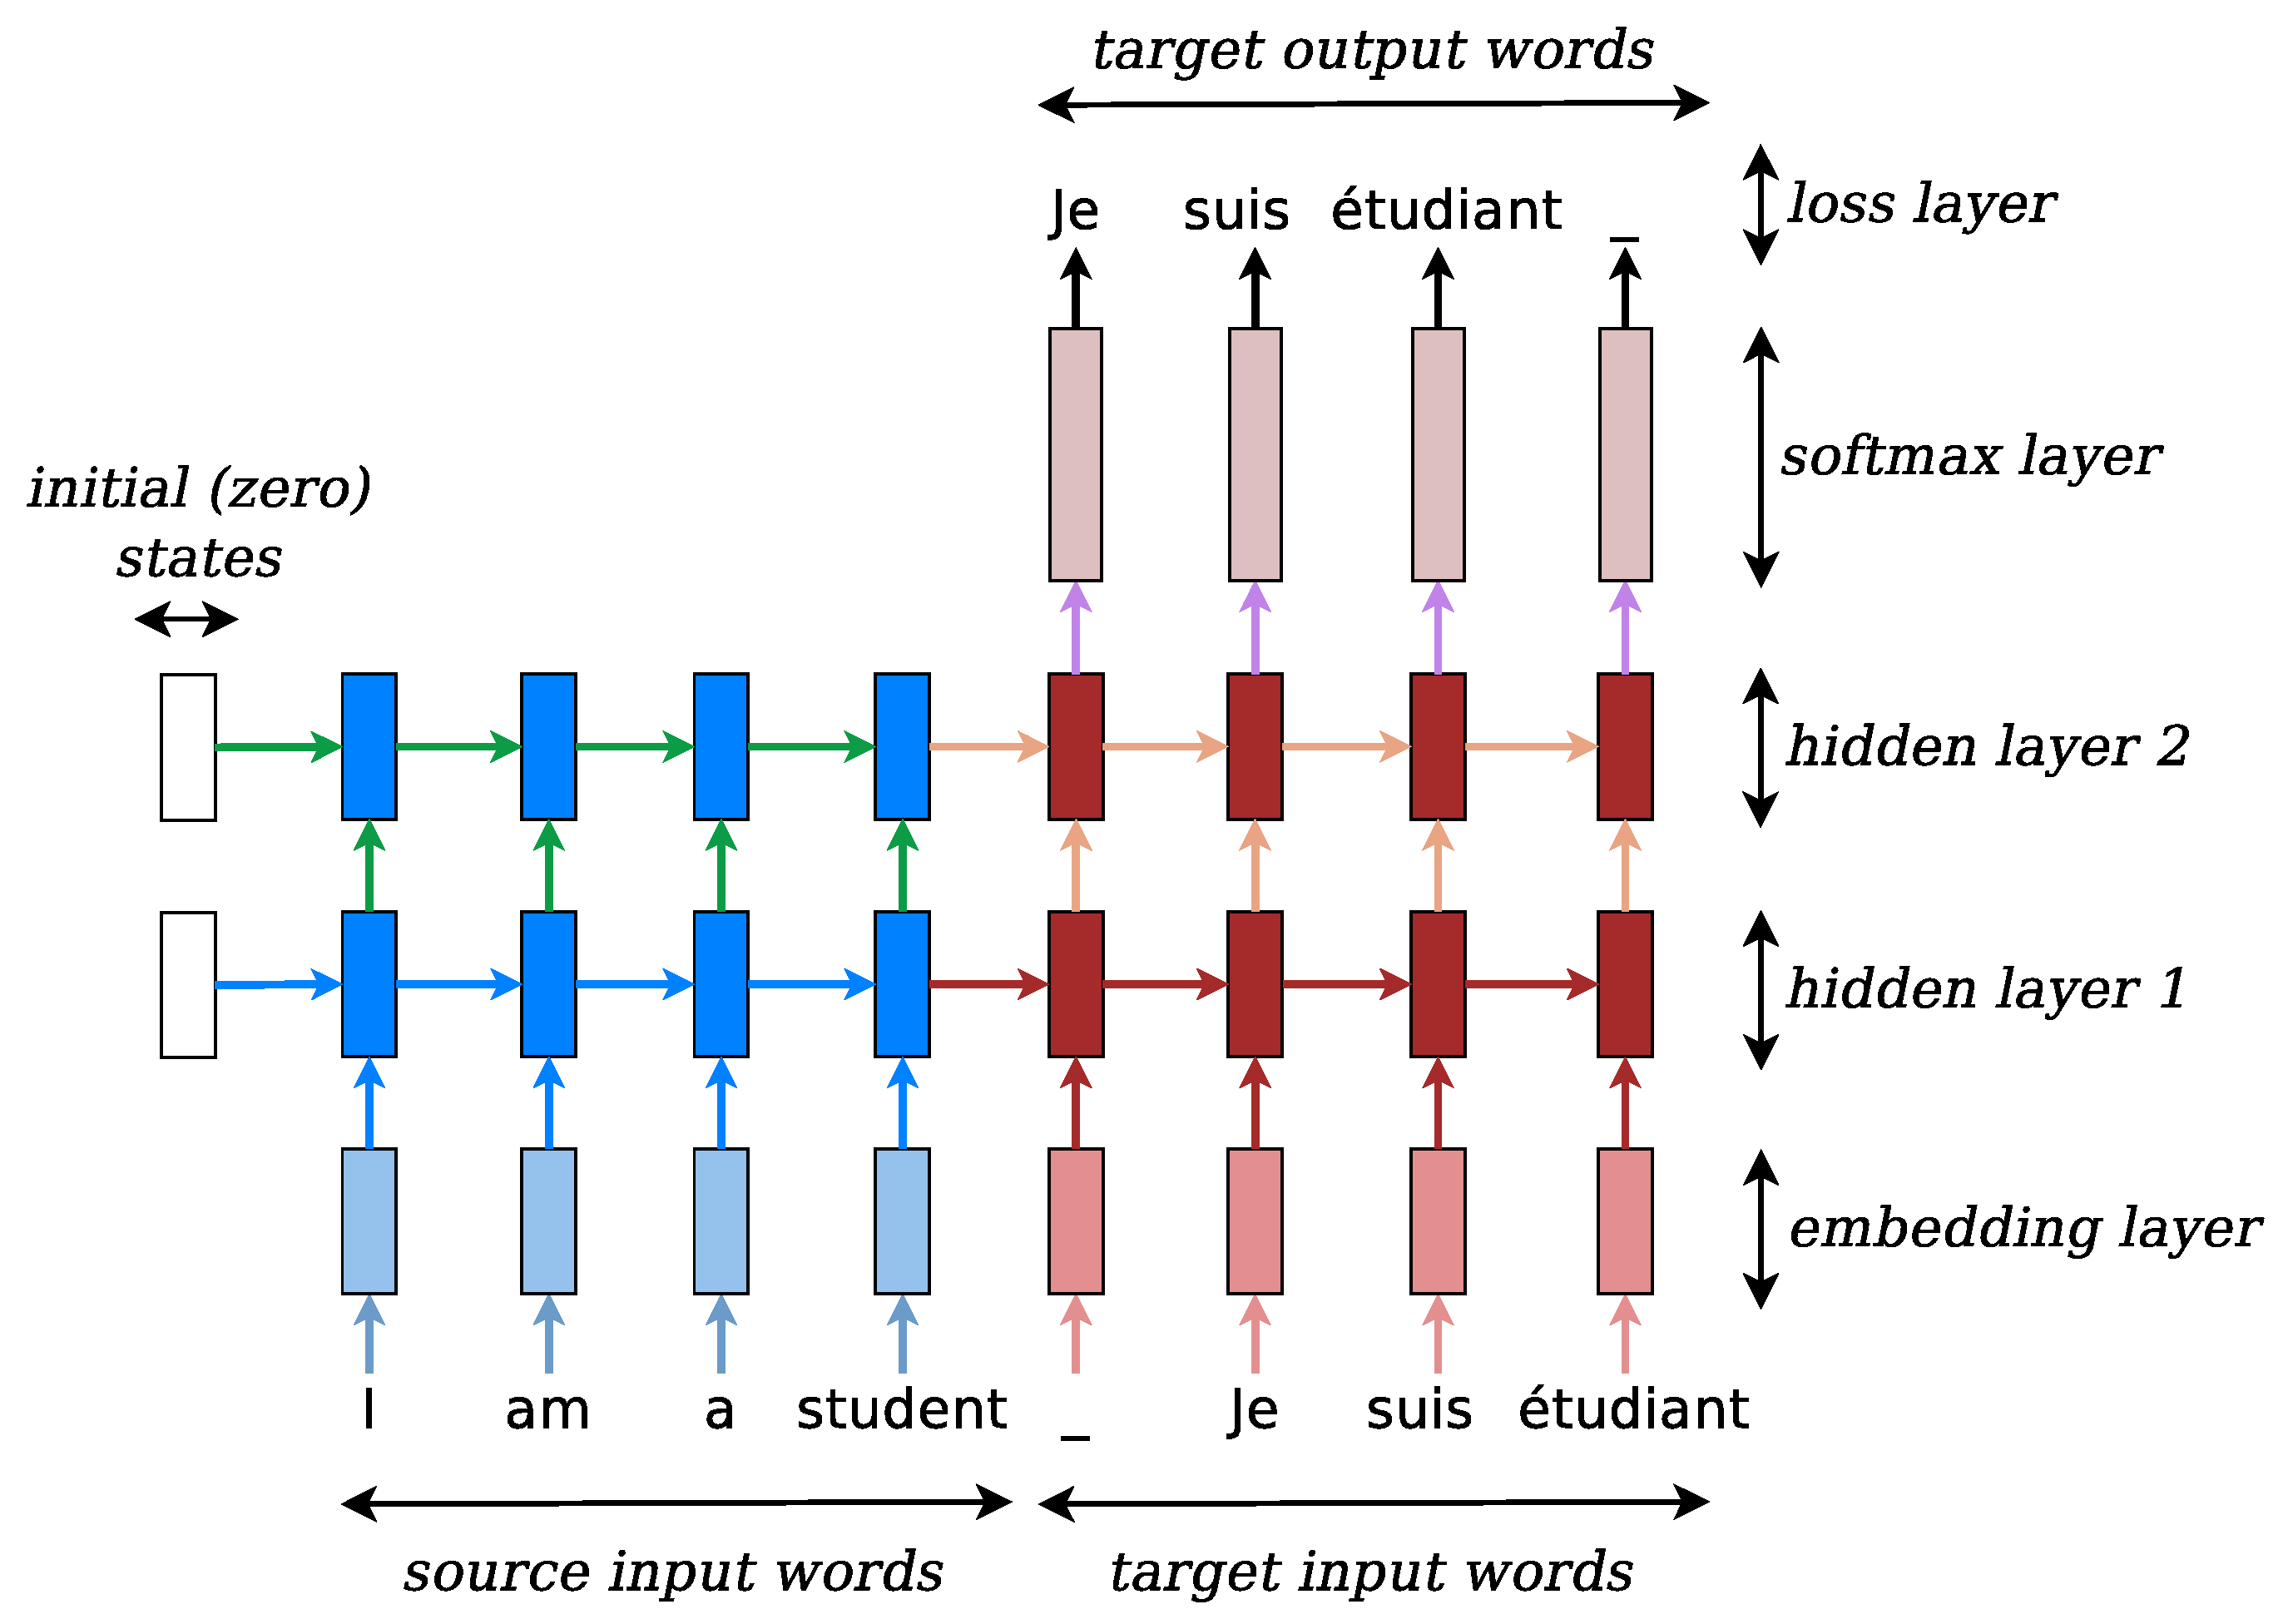
\includegraphics[width=0.8\textwidth, clip=true, trim= 0 0 0
0]{img/nmt_very_details.eps} % , angle=-90
\caption[Neural machine translation]{{\bf Neural machine translation} -- example of a deep recurrent
architecture proposed by \newcite{sutskever14} for
translating a source sentence \word{I am a student} into a target sentence
\word{Je suis \'{e}tudiant}. Here, \word{\texttt{\_}} marks the end of a sentence.
} 
\label{f:nmt_details}
\end{figure}

In this thesis, all our NMT models are deep multi-layer RNNs which are 
unidirectional and have LSTM as the recurrent unit. We show an example of
such model in Figure~\ref{f:nmt_details} though it should be easy to extend to
other RNN architectures. In this example, we train our model to translate a source sentence
\word{I am a student} into a target one \word{Je suis \'{e}tudiant}.
At a high level, our NMT models consist of two recurrent language models as
described in \secref{subsec:rlm}: the {\it encoder} RNN simply consumes the input
source words without making any prediction; the {\it decoder}, on the other
hand, processes
the target sentence while predicting the next words. 

In more detail, at the bottom layer, the encoder and decoder RNNs receive as
{\it input} the following: first,
the source sentence, then a boundary marker \word{\_} which indicates the
transition from the encoding to the decoding mode, and the target sentence. 
Given these discrete words, the model looks up the source and target
embeddings to retrieve the corresponding word representations.
For this {\it embedding layer} to work, a vocabulary is chosen for each language, and
often the top $V$ frequent words are selected.
%Thus, every word in the source or target vocabulary can be represented by a one-hot vector of length $V$.
%The source input sentence and target input sentence, represented as a sequence
%of one-hot vectors, are transformed into a sequence of word embeddings by the
%\emph{embedding} weights. 
These embedding weights, one set per language, are learned during training.
While one can choose to initialize embedding weights with pretrained word
representations, such as word2vec \cite{mikolov13nips} and Glove
\cite{pennington2014}, we found, in this thesis, that these
embeddings can be initialized randomly and learned from scratch given large training datasets.

%, are different for the source words and the target words.
%The word embeddings and all hidden layers are vectors of length $n$ (a chosen hyperparameter).

Once retrieved, the word embeddings are then fed as input into the main network, which consists
of two multi-layer RNNs `stuck together' --- an encoder for the source
language and a decoder for the target language. 
The encoder RNN uses zero vectors as its starting states. The decoder, on the
other hand, needs to have access to the source information, so one simple way to
achieve that is to
initialize it with the last hidden state of the encoder.\footnote{This is not the only way to initialize the decoder,
e.g., \newcite{cho14} connect the last encoder state to every timesteps in the
decoder.} In Figure~\ref{f:nmt_details}, we pass  
the hidden state at the source word \word{student} to the decoder side.
The \emph{feed-forward} (vertical) weights connect
the hidden unit from the layer below to the upper one; whereas, the
\emph{recurrent} (horizontal) weights transfer the history knowlege from the previous
timestep to the next one.
Often, we use different weights across the encoder and decoder as well as
across different layers; in the current example, we have 4 different LSTM
weight sets $\lstm$, detailed in \eq{e:lstm_notation}, over $\{\text{encoder,
decoder}\} \times \{1^{\text{st}}, 2^{\text{nd}} \text{ layer}\}$.
%The hidden state at the top layer of the decoder is fed through an
%\textit{attention} layer, which guides the translation by `paying attention' to relevant parts of the source sentence; 
%for more information see \cite{bahdanau2014neural} or Section 3 of \cite{luong2015effective}.
Finally, for each target word, the hidden state at the top layer is transformed by the
\emph{softmax} weights into a probability distribution over the target
vocabulary of size $V$ according to \eq{e:score} and \eq{e:prob}. 

\paragraph{Training}
Training neural machine translation is similar to training a recurrent
language model that we have discussed in \secref{sec:rnn} except that we need to
handle the conditioning part on source sentences.
The training objective for NMT is formulated as:
\begin{equation}
J = \sum_{(\src{},\tgt{}) \in \mathbb{D}} \nolimits -\log p(\tgt{}|\src{})
\label{e:j_t}
\end{equation}
Here, $\mathbb{D}$ refers to our parallel training corpus of source and target
sentence pairs $(x, y)$. Given the aforementioned NMT architecture,
computing the NMT loss for $(x, y)$ during the {\it forward} pass is
almost the same as how we compute the regular RNN loss on just $y$.
The only difference is that we have to first compute representations for the source
sentence $x$ to initialize the decoder RNN instead of just starting
from zero states. For the {\it backpropagation} phase, computing gradients for
the decoder is the same as what we have described in
Algorithm~\ref{a:lstm_bptt} for regular RNNs. The last hidden-state gradient
from the decoder is
passed back to the encoder. We then continue backpropating through the encoder
in a similar fashion as that of the decoder but without any prediction losses.

More concretely, we present in
\algo{a:nmt_forward} details in the forward pass of an NMT model which uses
a deep multi-layer LSTM architecture. Since the encoder and decoder share
many operations in common, we combine both the source sentence $x$ (length
$m_x$) and the target sentence $y$ (length $m_y$) together to form an input
sequence $s$ as shown in Line 1, which also includes the end-of-sentence marker
\word{\_}. We first start with the encoder weights and initial states
set to zero (Line~2-3). The algorithm switches to the decoder mode at time
$m_x + 1$ (Line~5). The same LSTM codebase (Line~8-11) is used for both the
encoder and decoder in which embeddings are first looked up for the input
$s_t$; after that, hidden states as well as LSTM cell memories are built from the
bottom layer to the top one (the $L^{\text{th}}$ layer). 
%The hidden state computed at one layer is used
%as input to the upper one according to Line~13. 
In Line~10, \texttt{LSTM} refers
to the entire formulation in
Eq~\ref{e:lstm_detailed}-\ref{e:lstm_detailed_output}, which one can easily
replace with other hidden units such as RNN and GRU. Lastly, on the decoder
side, the top hidden state is used to predict the next symbol $s_{t+1}$
(Line~13); then, a loss value $l_t$ and a probability distribution
$\prob{t}$ computed according to Eq~\ref{e:score}-\ref{e:prob} are returned.

\begin{algorithm}
$s \leftarrow [x, \text{\_}, y, \text{\_}]$ \tcp*{Length of $s$ is $m_x + 1 +
m_y + 1$}
$\W{e}, \lstm^{(1..L)} \leftarrow \W{e}^{\text{encoder}},
\lstm^{\text{encoder}}$ \tcp*{Encoder weights}
$\hid{0}^{(1..L)}, \mem{0}^{(1..L)} \leftarrow \bm{0}$ \tcp*{Zero init} %^{(1..L)}, \bm{0}^{(1..L)}$ \tcp*{Starting states and memories}
% Multi-layer 
%\For{$l=1 \rightarrow L$}{
%$\hid{0}^{(l)}, \mem{0}^{(l)} \leftarrow \bm{0}, \bm{0}$ \tcp*{Starting states and
%memories}
%}

\For{$t=1 \rightarrow (m_x + 1 + m_y)$}
{

\tcp{Decoder transition}
\If{$t == (m_x + 1)$}{
  $\W{e}, \lstm^{(1..L)} \leftarrow \W{e}^{\text{decoder}}, \lstm^{\text{decoder}}$ \; % \tcp{Decoder embeddings}
  %$\lstm^{(1..L)} \leftarrow \lstm^{\text{decoder}}$ \; % \tcp{Decoder multi-layer LSTMs}
}

\tcp{Multi-layer LSTM}
% x_t
$\hid{t}^{(0)} \leftarrow \text{\texttt{Emb\_LookUp}}(s_t, \W{e})$ \;
\For{$l=1 \rightarrow L$} {
  $\hid{t}^{(l)}, \mem{t}^{(l)} \leftarrow \text{\texttt{LSTM}}\paren{\hid{t-1}^{(l)},
  \mem{t-1}^{(l)}, \hid{t}^{(l-1)}, \lstm^{(l)}}$ \tcp*{LSTM hidden unit}
}

\tcp{Target-side prediction}
\If{$t \geq (m_x + 1)$}{
  $l_t, \prob{t} \leftarrow \text{\texttt{Predict}}(s_{t+1}, \hid{t}^{(L)},\W{hy})$ \;
}
}
\caption{NMT training algorithm -- {\it forward} pass.}
\label{a:nmt_forward}
\end{algorithm}


%% BPTT
Next, we describe details of the backpropagation step in \algo{a:nmt_backward}.
A quick glance through the algorithm reveals many similarities compared to the
forward pass algorithm except that we have reversed the procedue. First, we
start with the decoder weights and initialize all gradients to zero (Line~1-2).
At time $m_x$, we switch to the encoder mode while saving the currently
accumulated LSTM and embedding gradients for the decoder (Line~5-7). 
%Individual gradients are computed in Line~13-23. 
Thanks to the backpropagation
procedure presented earlier for LSTM, we can simplify the core NMT gradient
computation (Line~9-19) by making the following two referents: (a)
\texttt{Predict\_grad} (Line~2-4 of \algo{a:lstm_bptt}) which computes gradients for the target-side
losses with respect to the hidden states at the top layer and the softmax
weights $\W{hy}$; and (b) \texttt{LSTM\_grad} (Line~5-15 of
\algo{a:lstm_bptt}) which computes gradients for inputs to LSTM and the LSTM
weights per layer $\lstm^{(l)}$. It is important to note that in Lines 11 and 16 of
\algo{a:nmt_backward}, we add the gradients (flowed vertically from either the
loss or the upper LSTM layer) to the gradient of the below layer (which already
contains the gradient backpropagated horizontally)
instead of overriding it. Lastly, in Line 19, we perform
sparse updates on the corresponding embedding matrix for participating words
only.

\begin{algorithm}
% $s \leftarrow [x, \text{\_}, y, \text{\_}]$ \tcp*{Length of $s$ is $m_x + 1 + m_y + 1$}
$\W{e}, \lstm^{(1..L)} \leftarrow \W{e}^{\text{decoder}},
\lstm^{\text{decoder}}$ \tcp*{Decoder weights}
$d\hid{}^{(1..L)}, d\mem{}^{(1..L)}, d\lstm^{(1..L)}, d\W{e}, d\W{hy}
\leftarrow \bm{0}$ \tcp*{Zero init} %\; %\leftarrow \bm{0}^{(1..L)}, \bm{0}^{(1..L)}, \bm{0}, \bm{0}$ \tcp*{Starting gradients} % for memories} % m_x + 1 + m_y

\For{$t=(m_x + 1 + m_y) \rightarrow 1$} {

\tcp{Encoder transition}
\If{$t == m_x$}{
  $\W{e}, \lstm^{(1..L)} \leftarrow \W{e}^{\text{encoder}},
  \lstm^{\text{encoder}}$ \; %\tcp*{Encoder weights}
  $d\W{e}^{\text{decoder}}, d\lstm^{\text{decoder}} \leftarrow d\W{e},
  d\lstm^{(1..L)}$ \tcp*{Save decoder gradients}
  $d\lstm^{(1..L)}, d\W{e} \leftarrow \bm{0}$ \; %\tcp*{Zero init} %\;
}

\tcp{Target-side prediction}
\If{$t \geq (m_x + 1)$}{
  $d\hid{}, d\W{} \leftarrow
  \text{\texttt{Predict\_grad}}(s_{t+1}, \prob{t}, \hid{t}^{(L)},\W{hy})$\;
  % \texttt{Accumulate}$(d\W{hy})$;
  $d\hid{}^{(L)} \leftarrow d\hid{}^{(L)} + d\hid{}$\;
  $d\W{hy} \leftarrow d\W{hy} + d\W{}$\;
}

\tcp{Multi-layer LSTM}
\For{$l=L \rightarrow 1$} {
  %\tcp{The first two returning gradients are for the previous timestep}
  $d\hid{}^{(l)}, d\mem{}^{(l)}, d\x{}, d\bm{T} \leftarrow 
  \text{\texttt{LSTM\_grad}}\paren{d\hid{}^{(l)}, d\mem{}^{(l)}, \hid{t-1}^{(l)},
  \mem{t-1}^{(l)}, \hid{t}^{(l-1)}, \lstm^{(l)}}$ \;
  % \texttt{Accumulate}$(d\lstm^{(l)})$;
  $d\hid{}^{(l-1)} \leftarrow d\hid{}^{(l-1)} + d\x{}$\;
  $d\lstm^{(l)} \leftarrow d\lstm^{(l)} + d\bm{T}$\;
}
$d\W{e} \leftarrow \text{\texttt{Emb\_grad\_update}}(s_t, d\hid{}^{(0)}, d\W{e})$ \;

}
$d\W{e}^{\text{encoder}}, d\lstm^{\text{encoder}} \leftarrow d\W{e},
d\lstm^{(1..L)}$ \tcp*{Save encoder gradients}

\caption{NMT training algorithm -- {\it backpropagation} pass.}
\label{a:nmt_backward}
\end{algorithm}

% mention bucketing and batching

\subsection{Testing}
Having trained an NMT model, we, of course, need to be able to use it to
translate, or decode, unseen source sentences! This section explains a few different ways to 
accomplish this goal and how to decode with an ensemble of models.

The simplest strategy to translate a source sentence is to perform {\it greedy
decoding} which we illustrate in \figref{f:nmt_test}. The idea is simple: (a) we
first encode the source sentence,
\word{I am a student} in our example, similar to the training process; (b) the
decoding process is started as soon as
an end-of-sentence marker \word{\_} for the source sentence is fed as an input; and (c) for each
timestep on the decoder side,
we pick the most likely word (a greedy choice), e.g., \word{moi} has the highest
translation probability in the first
decoding step, then use it as an input to the next timestep, and continue
until the end-of-sentence marker \word{\_} is produced as an output symbol. Step
(c) is what makes testing different from training: unlike training in which
correct target words in $y$ are always fed as an input, testing, on the other
hand, uses words predicted by the model.

\begin{figure}[tbh!]
\centering
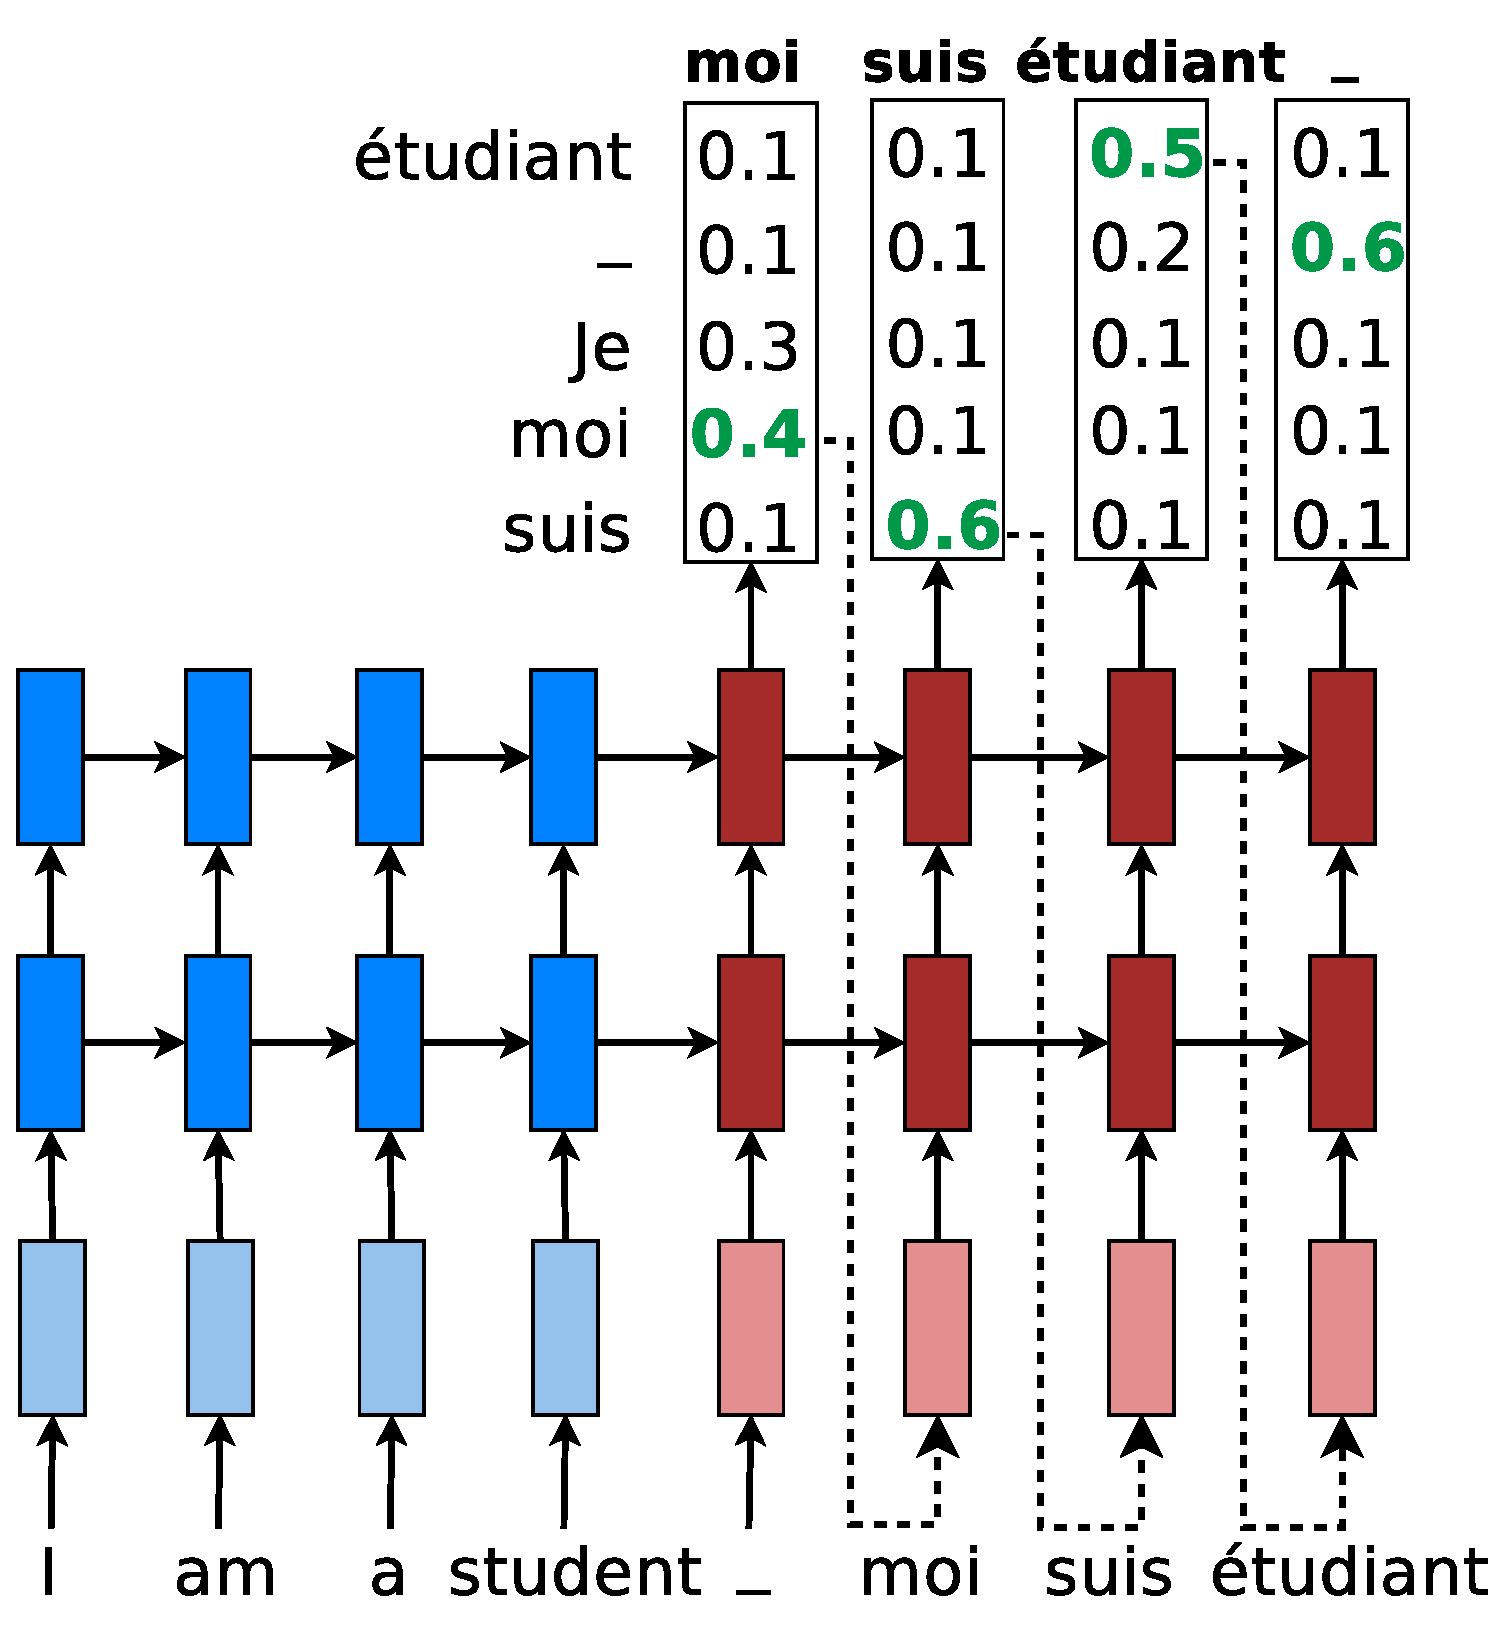
\includegraphics[width=0.6\textwidth, clip=true, trim= 0 0 0
0]{img/nmt_test.eps} % , angle=-90
\caption[Neural machine translation]{{\bf Greedy Decoding}
-- example of how a trained NMT model produces a translation for a
source sentence \word{I am a student} using greedy search.
} 
\label{f:nmt_test}
\end{figure}

More concretely, we adopt the NMT forward algorithm to arrive at the greedy
decoding strategy in \algo{a:nmt_greedy}. We present the greedy
algorithm in a slightly more abstract way by reusing elements of the NMT forward
pass in \algo{a:nmt_forward}. First, we run through the encoder in Line 1 to obtain a
representation $\hid{0}, \mem{0}$ for the source sentence $x$ (length $m_x$). We
then use the end-of-sentence marker \word{\_} as an input to start the decoding
process and restrict the final translation to have a maximum length of
$\alpha*m_x$.\footnote{We often set $\alpha$ to $1.5$} At each timestep on the
decoder side, we call \texttt{MultiLayerLSTM}, which refers to Line~8-11 in
\algo{a:nmt_forward}, to build up representations over $L$ stacking LSTM layers. The hidden
state at the top layer is used to compute the predictive distribution $\prob{t}$
from which we make a greedy choice to produce the index of the translation word
at that timestep (Line~7). The process ends when we have produced the marker
\word{\_} as a translation word or when the translation length exceeds the
length threshold.

\begin{algorithm}
$\hid{0}, \mem{0} \leftarrow \text{Encoder}(x, \W{e}^{\text{encoder}}, \lstm^{\text{encoder}})$ \;
$t \leftarrow 1$ \;
$y_1 \leftarrow \_$ \;
\While(\tcp*[f]{Length factor $\alpha \geq 1$}){$t \leq \alpha * m_x$} {
  $\hid{t}, \mem{t} \leftarrow \text{\texttt{MultiLayerLSTM}}\paren{\hid{t-1},
  \mem{t-1}, y_t, \W{e}^{\text{decoder}}, \lstm^{\text{decoder}}}$ \;

  $\prob{t} \leftarrow \text{\texttt{Softmax}}(\hid{t}^{(L)},\W{hy})$ \;
  $y_{t+1} \leftarrow \argmax_i \prob{t}(i)$ \tcp*{\bfit{Greedy} choice}
  \If(\tcp*[f]{Ending condition}){$y_{t+1} == \Index(\_)$} {
    break\;
  }

  $t \leftarrow t+1$
}
\Return $y_{2..t}$

\caption{NMT {\it greedy} decoding algorithm.}
\label{a:nmt_greedy}
\end{algorithm}



\chapter{Copy Mechanisms}
\label{c:copy}
Despite all of the advantages mentioned in the previous chapter, basic NMT systems are incapable of translating rare 
words because they have a fixed modest-sized vocabulary\footnote{ Due to the computationally intensive nature of the softmax, NMT systems often limit 
their vocabularies to be the top 30K-80K most frequent words in each language.}
which forces them to use the \unksym{} symbol to 
represent the large number of out-of-vocabulary (OOV) words, as illustrated in Figure~\ref{f:sent_pair}.
Unsurprisingly, both \newcite{sutskever14} and \newcite{bog15} have
observed that sentences with many rare words tend to be translated much more poorly than sentences
containing mainly frequent words.
Standard phrase-based systems \cite{koehn2007moses,chiang07hiero,cer10phrasal,dyer10cdec}, 
on the other hand, do not suffer from the rare word 
problem to the same extent because they can support a much larger vocabulary, 
and because their use of explicit alignments
and phrase tables allows for memorizing the translations 
of even extremely rare words. 

\begin{figure*}
\resizebox{10cm}{!}{
\setlength{\unitlength}{1.1cm}
\begin{picture}(10, 2.7) %(-3,-2)
\put(0,2){{\it en}: The \unkword{ecotax} portico in \unkword{Pont-de-Buis} , \ldots [truncated] \ldots , was taken down on Thursday morning}
\put(0,1){{\it fr}: \mbox{} Le \unkword{portique} \unkword{\'{e}cotaxe} de \unkword{Pont-de-Buis} , \ldots [truncated] \ldots , a \'{e}t\'{e} \unkword{d\'{e}mont\'{e}} jeudi matin}
\put(0,0){{\it nn}: Le \unksym{} de \unksym{} \`{a} \unksym{} , \ldots [truncated] \ldots , a \'{e}t\'{e} pris le jeudi matin}
\put(1.7,1.3){\line(2,1){1.2}} % portico
\put(3.0,1.3){\line(-2,1){1.2}} % ecotax 
\put(5.2,1.3){\line(-1,2){0.3}} % Pont-de-Buis
\put(10.8,1.3){\line(-1,1){0.6}} % taken
\put(10.8,1.3){\line(1,3){0.2}} % down
\put(12,1.3){\line(3,2){0.9}} % Thursday
\put(13,1.3){\line(2,1){1.2}} % morning
\end{picture}
}
\caption[Example of the rare word problem]{{\bf Example of the rare word problem} -- An English source sentence ({\it en}), a human translation to French ({\it fr}), and a translation produced by one of my neural network systems ({\it nn}) before handling OOV words. I highlight \unkword{words} that are unknown to my model. 
The token \unksym{} indicates an OOV word. 
I also show a few important alignments between the pair of sentences. 
}
\label{f:sent_pair}
\end{figure*}

Motivated by the strengths of the standard phrase-based system, I 
propose and implement a novel approach to address the rare word problem of NMTs.
My approach annotates the training corpus with 
explicit alignment information that enables the NMT system to emit, for each OOV word, a
``pointer'' to its corresponding word in the source sentence. This
information is later utilized in a post-processing step that translates
the OOV words using a dictionary or with the identity translation, if no translation is found.


Experimental results confirm that this approach is effective. On the English to French WMT'14
translation task, this approach provides an improvement of
up to \bestunkimp{} BLEU points (if the vocabulary is relatively small) 
over an equivalent NMT system that does not use this technique.
Moreover, my system is the first NMT that outperforms the winner of a WMT'14 task.


\section{Rare Word Models}
\label{sec:rare}
Despite the relatively large amount of work done on pure neural machine translation systems, 
there has been no work addressing the OOV problem in NMT systems, 
with the notable exception of \newcite{jean15}'s work which offered 
an efficient approximation to the softmax to accommodate for a very large vocabulary (500K words). However, even with a large vocabulary, the problem with rare words, e.g., names, numbers, etc., still persists, and \newcite{jean15} found that using techniques similar to ours are beneficial and complementary to their approach.

I propose to address the rare word problem by training the NMT system
to track the origins of the unknown words in the target sentences.  If
I knew the source word responsible for each unknown target word, I could introduce
a post-processing step that would replace each \unksym{} in the system's output
with a translation of its source word, using 
either a dictionary or the identity translation.  For example, in
Figure~\ref{f:sent_pair}, if the model knows that the second unknown token 
in the NMT (line {\it nn}) originates from the source
word \texttt{ecotax}, it can perform a word dictionary lookup to
replace that unknown token by \texttt{\'{e}cotaxe}. Similarly, an
identity translation of the source word \texttt{Pont-de-Buis} can be
applied to the third unknown token.

I present three annotation strategies that can easily be applied to any NMT system \cite{kal13,sutskever14,cho14}. 
I treat the NMT system as a black box and train it on a corpus annotated by one of the models below. 
First, the alignments are produced with an unsupervised aligner. 
Next, I use the alignment links to construct a word dictionary that will 
be used for the word translations in the post-processing step.\footnote{When a source word has multiple translations, I use the translation with the highest probability. These translation probabilities are estimated from the unsupervised alignment links. When constructing the dictionary from these alignment links, I add a word pair to the dictionary only if its alignment count exceeds 100.}
If a word does not appear in my dictionary, then I apply the identity translation.

The first few words of the sentence pair in Figure~\ref{f:sent_pair} (lines {\it en}
and {\it fr}) illustrate my models. 

\subsection{Copyable Model}
\label{subsec:copyable}
\begin{figure}
\resizebox{10.5cm}{!}{
\setlength{\unitlength}{1cm}
\begin{picture}(10, 1) %(-3,-2)
\put(0.5,0.7){en: The \unkcopy{1} portico in \unkcopy{2} \ldots}
\put(0.5,0){fr: \mbox{} Le \unknull{} \unkcopy{1} de \unkcopy{2} \ldots}
\end{picture}
}
\caption[Copyable Model]{ {\bf Copyable Model} -- an annotated example with two 
types of unknown tokens: ``copyable'' \unktext{n} and null \unknull{}.}
\label{f:copyable}
\end{figure}

In this approach, I introduce multiple tokens to represent the various unknown words in the 
source and in the target language, as opposed to using only one \unksym{} token. 
I annotate the OOV words in the source sentence
with \unktext{1}, \unktext{2}, \unktext{3}, in that order,
while assigning repeating unknown words identical tokens. 
The annotation of the unknown words in the target language is slightly more elaborate: (a) each 
unknown target word that is aligned to an unknown source word
is assigned the same unknown token (hence, the ``copy'' model) and 
(b) an unknown target word that has no 
alignment or that is aligned with a known word uses the special null token \unknull{}. 
See Figure~\ref{f:copyable} for an example.  This annotation enables us to 
translate every non-null unknown token.

\subsection{Positional All Model (PosAll)}
The copyable model is limited by its inability to translate unknown 
target words that are aligned to \emph{known} words in the source sentence, such as the pair of 
words, ``portico'' and ``portique'', in my running example. 
The former word is known on the source sentence; whereas latter is not, so it is labelled with \unknull{}.
This happens often since the source vocabularies of my models tend to be much 
larger than the target vocabulary since a large source vocabulary is cheap.
This limitation motivated us to develop an annotation model that includes the complete 
alignments between the source and the target sentences, which is straightforward to obtain
 since the complete alignments are available at training time.  

Specifically, I return to using only a single universal \unksym{} token. 
However, on the target side, 
I insert a positional token \postext{d} after every word. Here, $d$ indicates a relative position 
($d=-7,\ldots,-1,0,1,\ldots,7$) to denote that a target word at position $j$ is aligned 
to a source word 
at position $i=j-d$. Aligned words that are too far apart are considered unaligned, and 
unaligned words are annotated
with a null token \postext{n}. My annotation is illustrated in 
Figure~\ref{f:pos_all}.

\begin{figure}
\resizebox{10.5cm}{!}{
\setlength{\unitlength}{1cm}
\begin{picture}(10, 1) %(-3,-2)
\put(0,0.7){en: The \unksym{} portico in \unksym{} \ldots} 
\put(0,0){fr: \mbox{} Le \pos{0} \unksym{} \pos{-1} \unksym{} \pos{1} de \posnull{} \unksym{} \pos{-1} \ldots}
\end{picture}
}
\caption[Positional All Model]{ {\bf Positional All Model} -- an example of the PosAll model. Each word is followed by the relative positional tokens \postext{d} or the null token \posnull{}. }
\label{f:pos_all}
\end{figure}

\subsection{Positional Unknown Model (PosUnk)}

The main weakness of the PosAll model is that it doubles the length of the target sentence. This
makes learning more difficult and slows the speed of parameter updates by a factor of two.
However, given that my post-processing step is concerned only with the alignments of the unknown words,
so it is more sensible to only annotate the unknown words. 
This motivates my {\it positional unknown} model which uses \unkpostext{d} 
tokens (for $d$ in $-7,\ldots,7$ or $\emptyset$) to simultaneously 
denote (a) the fact that a word is unknown and (b) its relative position $d$ with respect to its aligned source word. 
Like the PosAll model, I use the symbol \unkpos{\emptyset} for unknown target words that do not have an alignment. 
I use the universal \unksym{} for all unknown tokens in the source language. See Figure~\ref{f:pos_unk} for an annotated example.

\begin{figure}[tbh!]
\resizebox{10.5cm}{!}{
\setlength{\unitlength}{1cm}
\begin{picture}(10, 1) %(-3,-2)
\put(0,0.7){en: The \unksym{} portico in \unksym{} \ldots} 
\put(0,0){fr: \mbox{} Le \unkpos{1} \unkpos{-1} de \unkpos{1} \ldots}
\end{picture}
}
\caption[Positional Unknown Model]{ {\bf Positional Unknown Model} -- 
an example of the PosUnk model: only aligned unknown words are annotated with the \unkpostext{d} tokens.}
\label{f:pos_unk}
\end{figure}

It is possible that despite its slower speed, the PosAll model will learn better alignments because 
it is trained on many more examples of words and their alignments. 
However, I show that this is not the case (see $\S$\ref{subsec:rare_model_compare}).


\section{Experiments}
\label{sec:exp}
I evaluate the effectiveness of my OOV models on the WMT'14 English-to-French translation 
task. Translation quality is measured with the BLEU metric \cite{Papineni02bleu} on the newstest2014 test set (which has 3003 sentences).

\subsection{Training Data}

To be comparable with the results reported by previous work on neural machine translation systems
\cite{sutskever14,cho14,bog15}, I train my models on 
the same training data of 12M parallel sentences (348M French and 304M English words), obtained from \cite{wmt14_en_fr}. 
The 12M subset was selected 
from the full WMT'14 parallel corpora using the method proposed in \newcite{Axelrod:2011:DAV}.%\footnote{\url{http://www-lium.univ-lemans.fr/~schwenk/cslm_joint_paper/}.}

Due to the computationally intensive nature of the naive softmax,
I limit the French vocabulary (the {\it target} language) 
to the either the 40K or the 80K most frequent French words. On the {\it source} side, 
I can afford a much larger vocabulary, so I use the 200K most frequent English words. 
The model treats all other words as unknowns.\footnote{When the French vocabulary has 40K words, there are
on average 1.33 unknown words per sentence on the target side of the test set.}

I annotate my training data using the three schemes described in the previous section. The alignment 
is computed with the Berkeley aligner \cite{liang06alignment} using its default settings.
I discard sentence pairs in which the source or the target sentence exceed 100 tokens.

\subsection{Training Details}
\label{subsec:train_details}
\begin{sloppypar}
My training procedure and hyperparameter choices are similar to those used by
\newcite{sutskever14}. In more details, I train multi-layer deep LSTMs, each of which has 
1000 cells, with 1000 dimensional embeddings. Like \newcite{sutskever14}, 
I reverse the words in the source sentences which 
has been shown to improve LSTM memory utilization and results in better translations of long sentences. 
My hyperparameters can be summarized as follows: (a) the parameters are initialized uniformly  
in [-0.08, 0.08] for 4-layer models and [-0.06, 0.06] for 6-layer models, (b) SGD has a fixed learning rate of 0.7, (c) I train for 8 epochs (after
5 epochs, I begin to halve the learning rate every 0.5 epoch), (d) the size of the mini-batch is 128, 
and (e) I rescale the normalized gradient to ensure that its norm does not
exceed 5 \cite{pascanu13}.
\end{sloppypar}

I also follow the GPU parallelization scheme proposed in \cite{sutskever14}, allowing us to  
reach a training speed of 5.4K words per second to train a depth-6 model with 200K source and 80K target vocabularies; whereas \newcite{sutskever14} achieved 6.3K words per 
second for a depth-4 models with 80K source and target vocabularies.
Training takes about 10-14 days on an 8-GPU machine.

\subsection{A note on BLEU scores}
I report BLEU scores based on both: (a) {\it detokenized} translations, i.e., WMT'14 style, to be comparable with results reported on the WMT website\footnote{\url{http://matrix.statmt.org/matrix}} and (b) {\it tokenized translations}, so as to be consistent with previous work \cite{cho14,bog15,wmt14_en_fr,sutskever14,jean15}.\footnote{The \texttt{tokenizer.perl} and \texttt{multi-bleu.pl} scripts are used to tokenize and score translations.}

The existing WMT'14 state-of-the-art system \cite{durrani-EtAl:2014:W14-33} achieves a detokenized BLEU score of 35.8 on 
the newstest2014 test set for English to French language pair (see Table~\ref{t:results_wmt}). In terms of the tokenized BLEU, its performance is 37.0 points (see Table~\ref{t:results}).
\begin{table}[tbh!]
\centering
\begin{tabular}{l|c}
\bf{System} & \bf{BLEU}\\
  \hline
Existing SOTA \cite{durrani-EtAl:2014:W14-33} & 35.8\\
%  \hline
%Ensemble of 8 LSTMs & 80K & 36M & \bestbleu{}\\
  \hline
Ensemble of 8 LSTMs + PosUnk  & {\bf \bestbleuunkwmt{}}\\
\end{tabular}
\caption[Detokenized BLEU on newstest2014]{{\bf Detokenized BLEU on newstest2014} -- translation results of the existing state-of-the-art system and my best system.}
\label{t:results_wmt}
\end{table}


\subsection{Main Results}
\begin{sloppypar}
I compare my systems to others, including the then state-of-the-art MT system \cite{durrani-EtAl:2014:W14-33},
recent end-to-end neural systems, as well as phrase-based baselines with neural components.
\end{sloppypar}

The results shown in Table~\ref{t:results} demonstrate that my unknown word translation technique (in particular, the PosUnk model) significantly improves the translation quality for both the individual (non-ensemble) LSTM models and the ensemble models.\footnote{
For the 40K-vocabulary ensemble, I combine 5 models with 4 layers and 3 models
with 6 layers. For the 80K-vocabulary ensemble, I combine 3 models with 4
layers and 5 models with 6 layers. Two of the depth-6 models are regularized
with dropout, similar to \newcite{zaremba14} with the dropout probability set to 0.2.} 
For 40K-word vocabularies, the performance gains are in the range of 2.3-2.8 BLEU points. With larger vocabularies (80K), the performance gains are diminished, but my technique can still provide a nontrivial gains of 1.6-1.9 BLEU points. 

\begin{table*}[tbh!]
\centering
\resizebox{15cm}{!}{
\begin{tabular}{l|c|c|l}
\bf{System} & \bf{Vocab} & {\bf Corpus} & \bf{BLEU}\\
  \hline
State of the art in WMT'14 \cite{durrani-EtAl:2014:W14-33} & All & 36M & {\bf 37.0}\\
  \hline
\multicolumn{4}{c}{{\it Standard MT + neural components}}\\
  \hline
\newcite{wmt14_en_fr} -- neural language model & All & 12M & 33.3\\ % 
\newcite{cho14}-- phrase table neural features & All & 12M & 34.5\\ % 
\newcite{sutskever14} -- 5 LSTMs, reranking 1000-best lists & All & 12M & 36.5\\ %
  \hline
\multicolumn{4}{c}{{\it Existing end-to-end NMT systems}}\\
  \hline
\newcite{bog15} -- single gated RNN with search & 30K & 12M & 28.5\\
\newcite{sutskever14} -- 5 LSTMs & 80K & 12M & 34.8\\
\newcite{jean15} -- 8 gated RNNs with search + UNK replacement & 500K & 12M & 37.2\\
  \hline
\multicolumn{4}{c}{{\it My end-to-end NMT systems }}\\
  \hline
Single LSTM with 4 layers  & 40K & 12M & 29.5\\ %(perplexity 4.69)
Single LSTM with 4 layers + PosUnk & 40K & 12M & 31.8 (+2.3) \\
Single LSTM with 6 layers & 40K & 12M & 30.4\\ %(perplexity 4.64) 
Single LSTM with 6 layers + PosUnk & 40K & 12M & 32.7 (+2.3) \\
Ensemble of 8 LSTMs & 40K & 12M & 34.1 \\
Ensemble of 8 LSTMs + PosUnk & 40K & 12M & 36.9 (+2.8)\\
  \hline
Single LSTM with 6 layers & 80K & 36M & 31.5\\ %(perplexity 4.64) 
Single LSTM with 6 layers + PosUnk & 80K & 36M & 33.1 (+1.6) \\
Ensemble of 8 LSTMs & 80K & 36M & \bestbleu{}\\
Ensemble of 8 LSTMs + PosUnk & 80K & 36M & {\bf \bestbleuunk{} (+\unkimp{})}\\
\end{tabular}
}
\caption[Tokenized BLEU on newstest2014]{{\bf Tokenized BLEU on newstest2014} --  Translation results of various systems which differ in terms of: (a) the architecture, (b) the size of the vocabulary used, and (c) the training corpus, either using the full WMT'14 corpus of 36M sentence pairs or a subset of it with 12M pairs. 
I highlight the performance of my best system in bolded text and state the improvements obtained by our technique of handling rare words (namely, the PosUnk model). Notice that, for a given vocabulary size, the more accurate systems achieve a greater improvement from the post-processing step.  This is the case because the more accurate models are able to pin-point the origin of an unknown
word with greater accuracy, making the post-processing more useful.
}
\label{t:results}
\end{table*}


It is interesting to observe that our approach is more useful for ensemble models as compared to the individual ones. 
This is because the usefulness of the PosUnk model directly
depends on the ability of the NMT to correctly locate, for a given OOV target word, its corresponding word in the source sentence.  An ensemble of large models identifies these source words with greater accuracy.  This is why for the same vocabulary size, better models obtain a greater performance gain our post-processing step. 
Except for the very recent work of \newcite{jean15} that employs a similar unknown treatment strategy\footnote{Their unknown replacement method and mine both track the locations of target unknown words and use a word dictionary to post-process the translation. However, the mechanism used to achieve the ``tracking'' behavior is different. \newcite{jean15}'s uses the attentional mechanism to track the origins of all target words, not just the unknown ones. In contrast, I only focus on tracking unknown words using unsupervised alignments. My method can be easily applied to any sequence-to-sequence models since I treat any model as a blackbox and manipulate only at the input and output levels.} as mine, our best result of \bestbleuunk{} BLEU outperforms all other NMT systems by a large margin, and 
more importantly, our system has established a new record on the WMT'14 English to French translation.

\section{Analysis}
\label{sec:analysis}
I analyze and quantify the improvement obtained by my rare word translation approach and provide a detailed 
comparison of the different rare word techniques proposed in Section~\ref{sec:rare}. I also examine the effect of 
depth on the LSTM architectures and demonstrate a strong correlation between perplexities and BLEU scores. I also highlight 
a few translation examples where my models succeed in correctly translating OOV words, and present 
several failures.

\subsection{Rare Word Analysis}
\begin{sloppypar}
To analyze the effect of rare words on translation quality, 
I follow Sutskever et al.~\cite{sutskever14} and sort sentences in 
newstest2014 by the average inverse frequency of their words. 
I split the test sentences into groups where the sentences within each group have a comparable number of rare words
 and evaluate each group independently. I evaluate my 
systems before and after translating the OOV words and compare with 
the standard MT systems -- I use the best system from the WMT'14 contest \cite{durrani-EtAl:2014:W14-33},
and neural MT systems -- I use the ensemble systems described in \cite{sutskever14} and Section~\ref{sec:exp}.
\end{sloppypar}

Rare word translation is challenging for neural machine translation systems as
shown in Figure~\ref{f:rare}. Specifically, the translation quality of my
model before applying the postprocessing step is shown by the green curve, and the current
best NMT system \cite{sutskever14} is the purple curve. While \cite{sutskever14}
produces better translations for sentences with frequent words (the left part of the
graph), they are worse than best system (red curve)
on sentences with many rare words (the right side of the graph). When applying my
unknown word translation technique (purple curve), I
significantly improve the translation quality of my NMT: 
for the last group of 500 sentences which have the greatest proportion of 
OOV words in the test set, I increase the BLEU score of my system by 
\imprare{} BLEU points. Overall, my rare word translation model 
interpolates between the SOTA system and the system
of \newcite{sutskever14},  which allows us to outperform the winning entry of WMT'14
on sentences that consist predominantly of frequent words and approach its performance on sentences
with many OOV words.
\begin{figure}
\centering
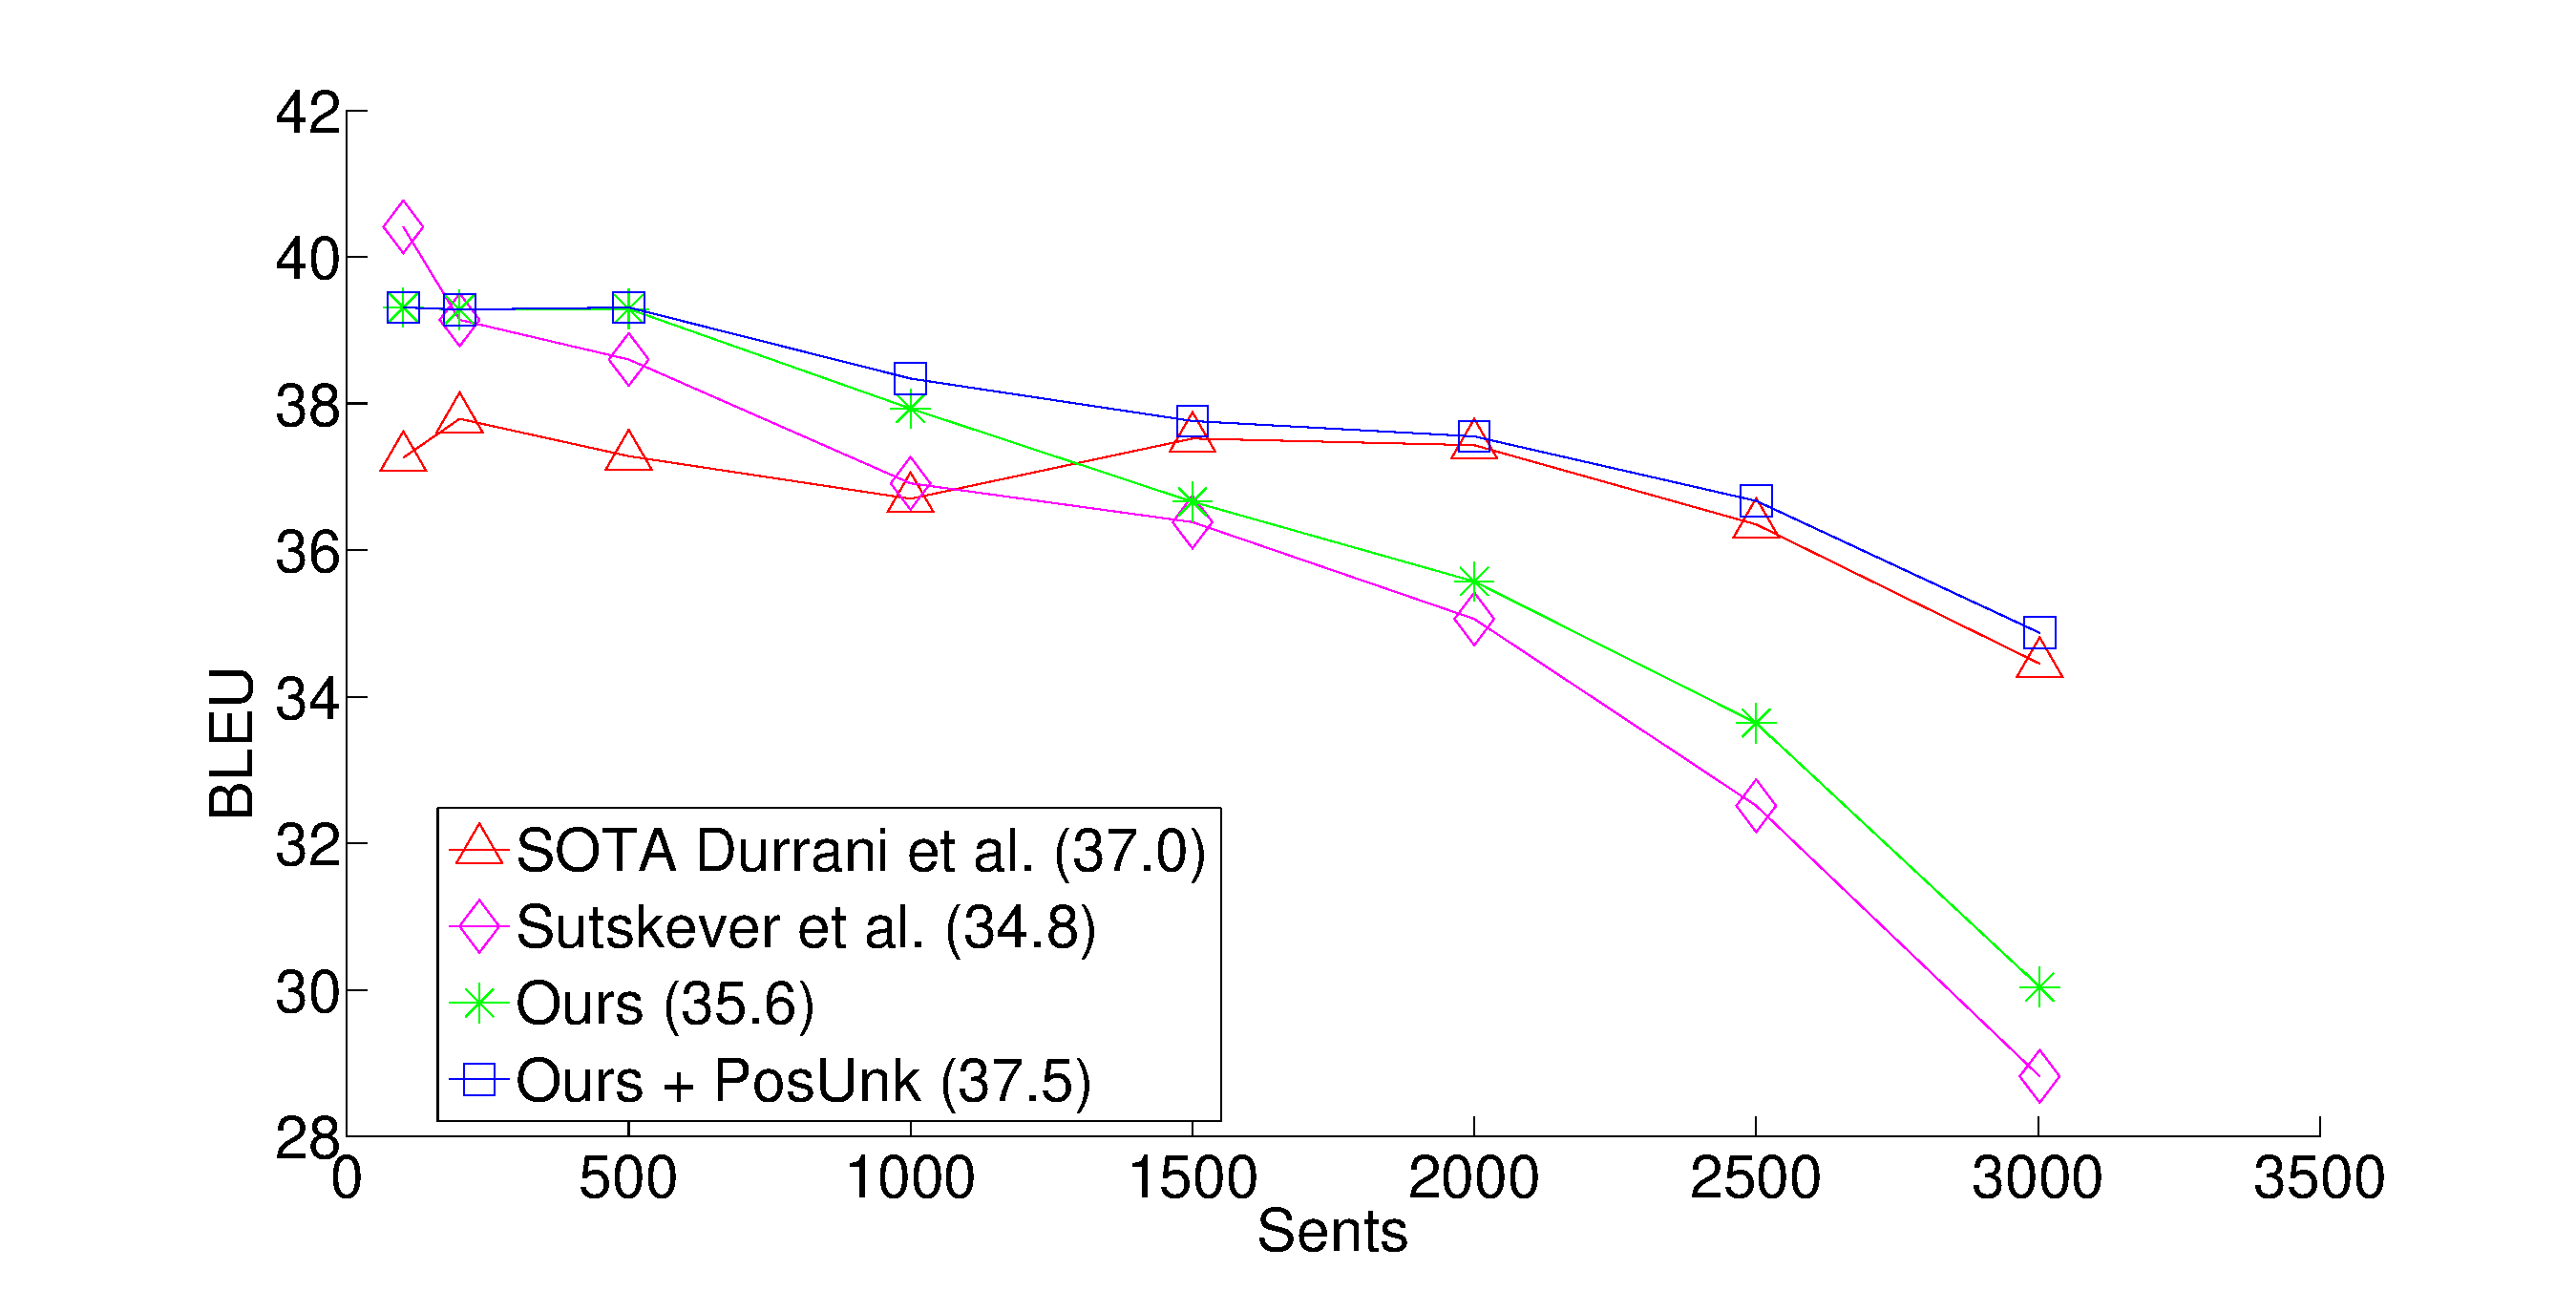
\includegraphics[width=0.7\textwidth, clip=true, trim= 95 0 230 0]{img/3-rare} % , angle=-90
\caption[Rare word translation]{{\bf Rare word translation} -- 
On the x-axis, I order newstest2014 sentences by their {\it average frequency rank} and divide the sentences into groups 
of sentences with a comparable prevalence of rare words. 
I compute the BLEU score of each group independently.} 
\label{f:rare}
\end{figure}


\subsection{Rare Word Models}
\label{subsec:rare_model_compare}

I examine the effect of the different rare word models presented in
Section~\ref{sec:rare}, namely: (a) {\it Copyable} -- which aligns the unknown
words on both the input and the target side by learning to copy indices, (b) the Positional All
({\it PosAll}) -- which predicts the aligned source positions for every target
word, and (c) the Positional Unknown ({\it PosUnk}) -- which predicts the aligned
source positions for only the unknown target words.\footnote{In this section and in section~\ref{subsec:effects},
all models are trained on the unreversed sentences, and I use the following hyperparameters: 
I initialize the parameters uniformly in [-0.1, 0.1], the learning rate is 1, the maximal gradient norm is 1, 
with a source vocabulary of 90k words, and a target vocabulary of 40k (see Section~\ref{subsec:train_details} for more details).
While these LSTMs do not achieve the best possible performance, it is still useful to analyze them.}
It is also interesting to measure the improvement obtained when no alignment information is used during training.
As such, I include a baseline model with no alignment knowledge ({\it NoAlign}) in which I simply assume that the $i^{\textrm{th}}$ unknown word on the target
sentence is aligned to the $i^{\textrm{th}}$ unknown word in the source sentence.

\begin{figure}
\centering
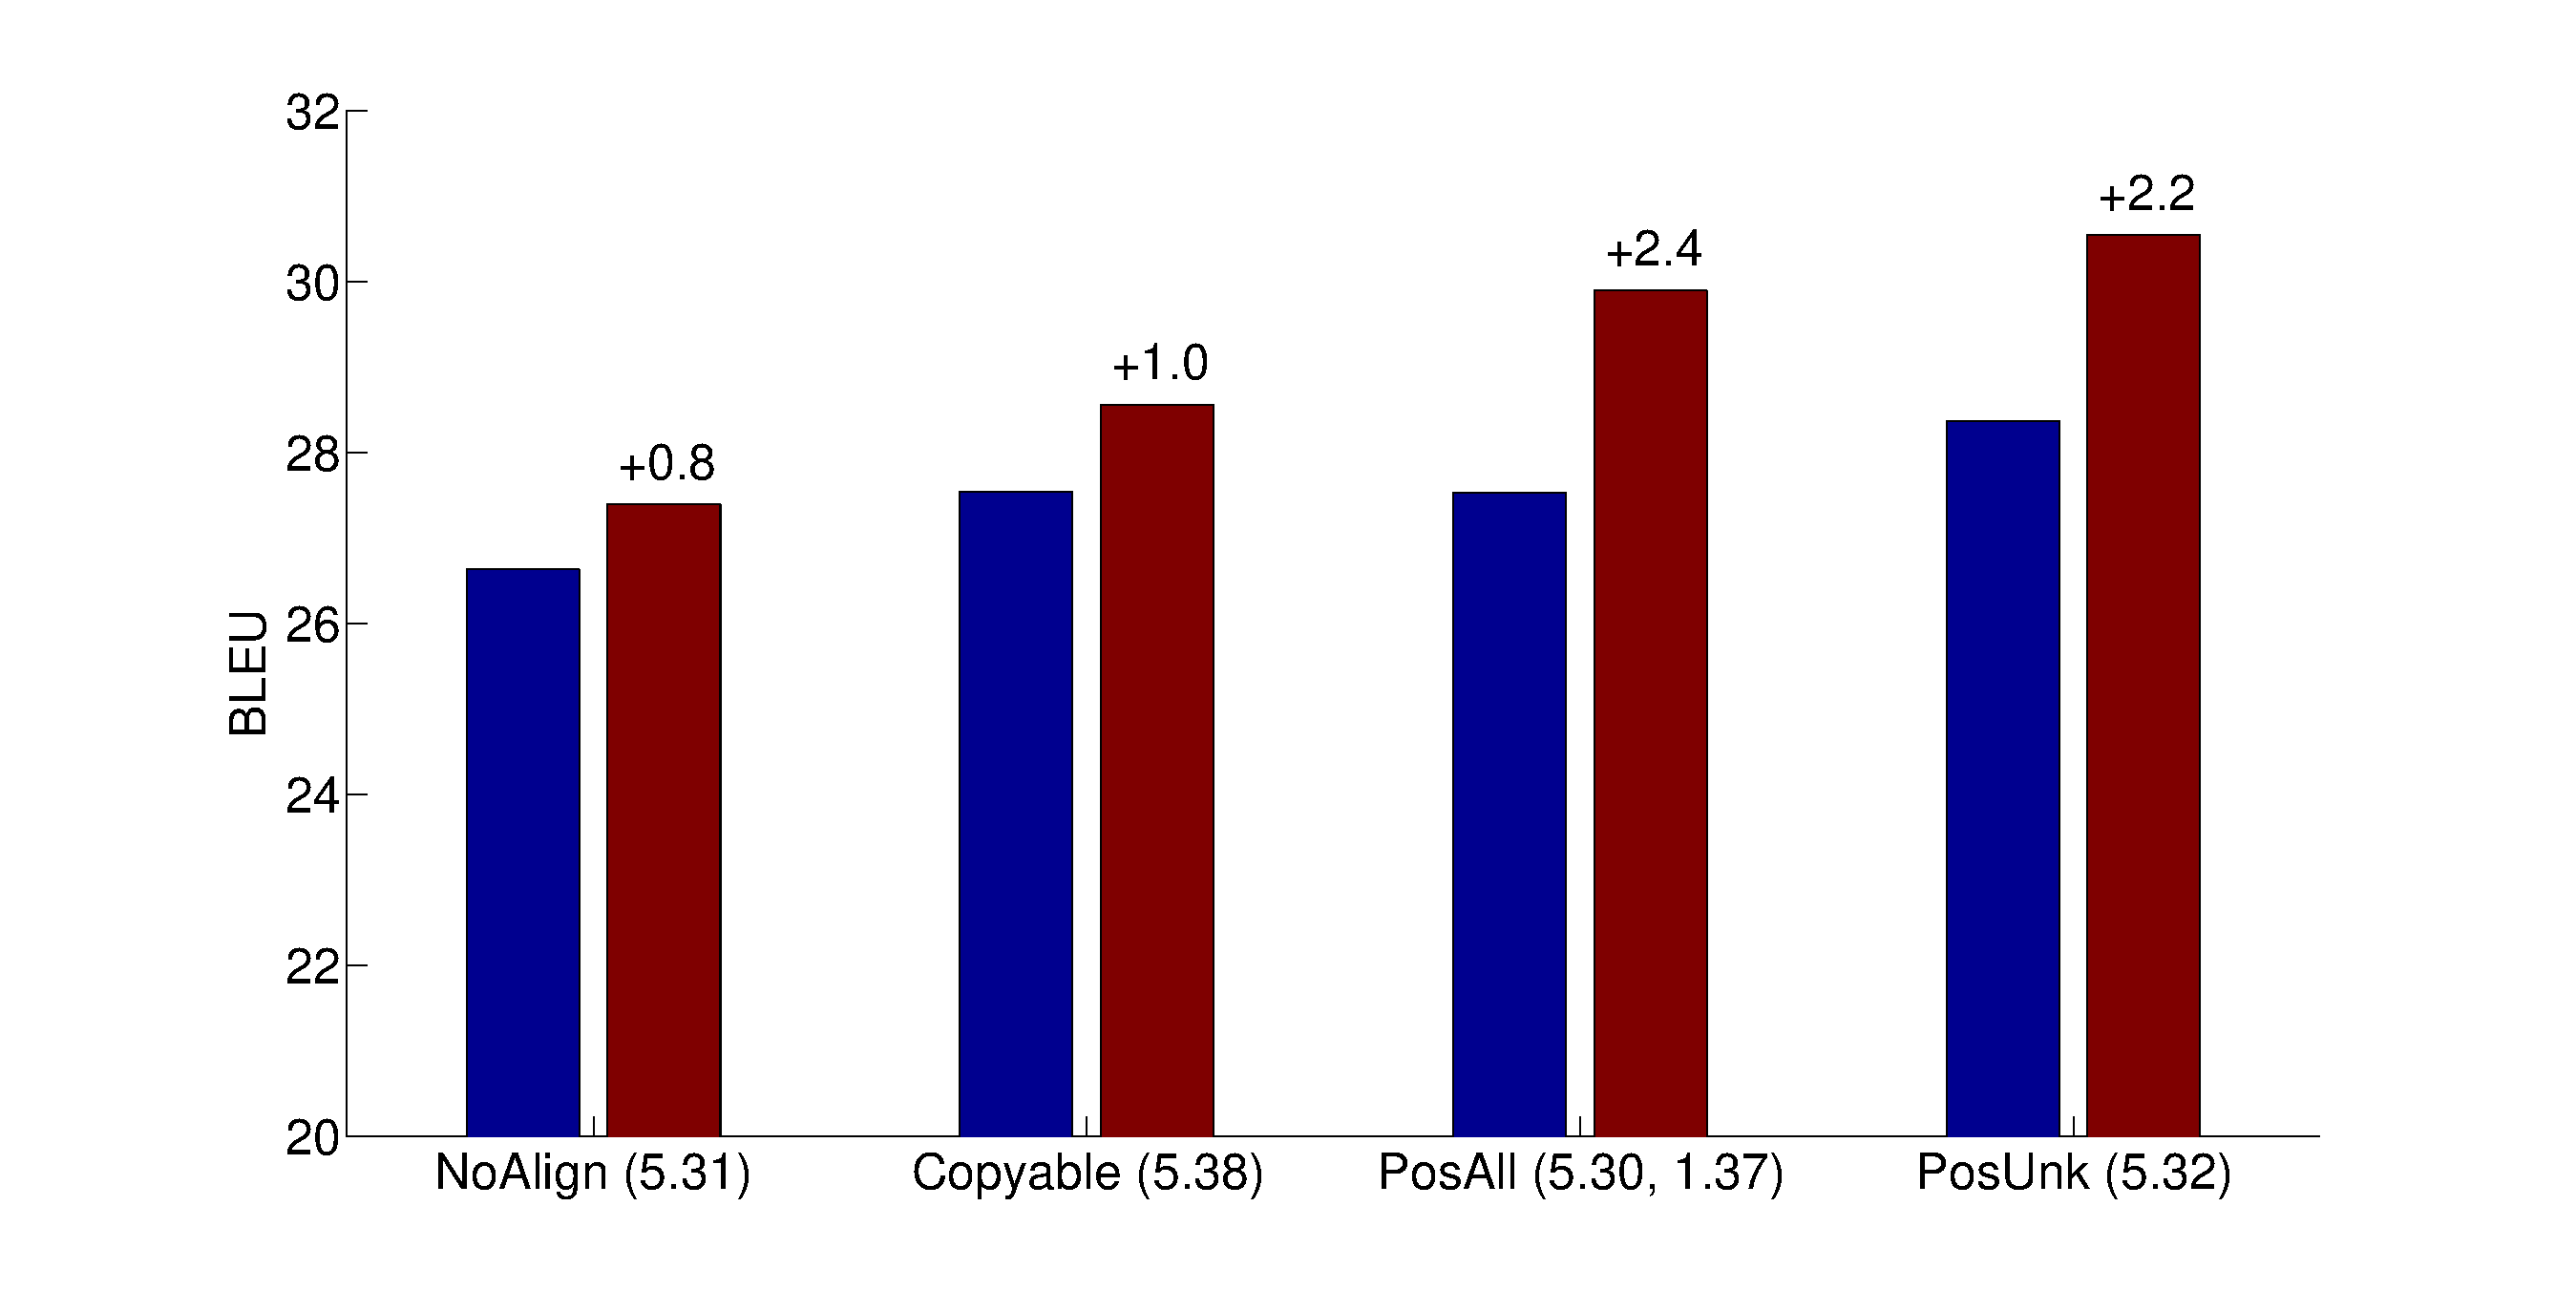
\includegraphics[width=0.7\textwidth, clip=true, trim= 105 0 140 0]{img/3-compare} % , angle=-90
\caption[Rare word models]{{\bf Rare word models} -- 
translation performance of 6-layer LSTMs:
a model that uses no alignment ({\it NoAlign}) 
and the other rare word models ({\it Copyable, PosAll, PosUnk}). 
For each model, I show results before ({\it left}) and after ({\it right}) the rare word translation as well as the perplexity (in parentheses).
For {\it PosAll}, I report the perplexities of predicting the words and the positions.} 
\label{f:compare}
\end{figure}

 
From the results in Figure~\ref{f:compare}, a simple monotone
alignment assumption for the {\it NoAlign} model yields a modest gain of
0.8 BLEU points. If I train the model to predict the alignment, then the {\it Copyable} model
offers a slightly better gain of 1.0 BLEU. Note, however, that English
and French have similar word order structure, so it would be
interesting to experiment with other language pairs, such as English and
Chinese, in which the word order is not as monotonic. These harder language pairs 
potentially imply a smaller gain for the NoAlign model and a larger
gain for the Copyable model. 
I leave it for future work.

The positional models ({\it PosAll} and {\it PosUnk}) 
improve translation performance by more than 2 BLEU points. 
This proves that the limitation of the copyable model, which forces
it to align each unknown output word with an unknown input word, is considerable.  
In contrast, the positional models can align the unknown target words with any source word,
and as a result, post-processing has a much stronger effect. 
The PosUnk model achieves better translation results than
the PosAll model which suggests that it is easier to train the LSTM on shorter sequences. 

\subsection{Other Effects}
\label{subsec:effects}
{\bf Deep LSTM architecture} --  I compare PosUnk models trained with different number of layers (3, 4, and 6). 
I observe that the gain obtained by the PosUnk model increases in tandem with the overall accuracy of the model, which is consistent 
with the idea that larger models can point to the appropriate source word more accurately.
Additionally, I observe that on average, each extra LSTM layer provides roughly 1.0 BLEU point improvement as demonstrated in Figure~\ref{f:depth}. 

\begin{figure}[tbh!]
\centering
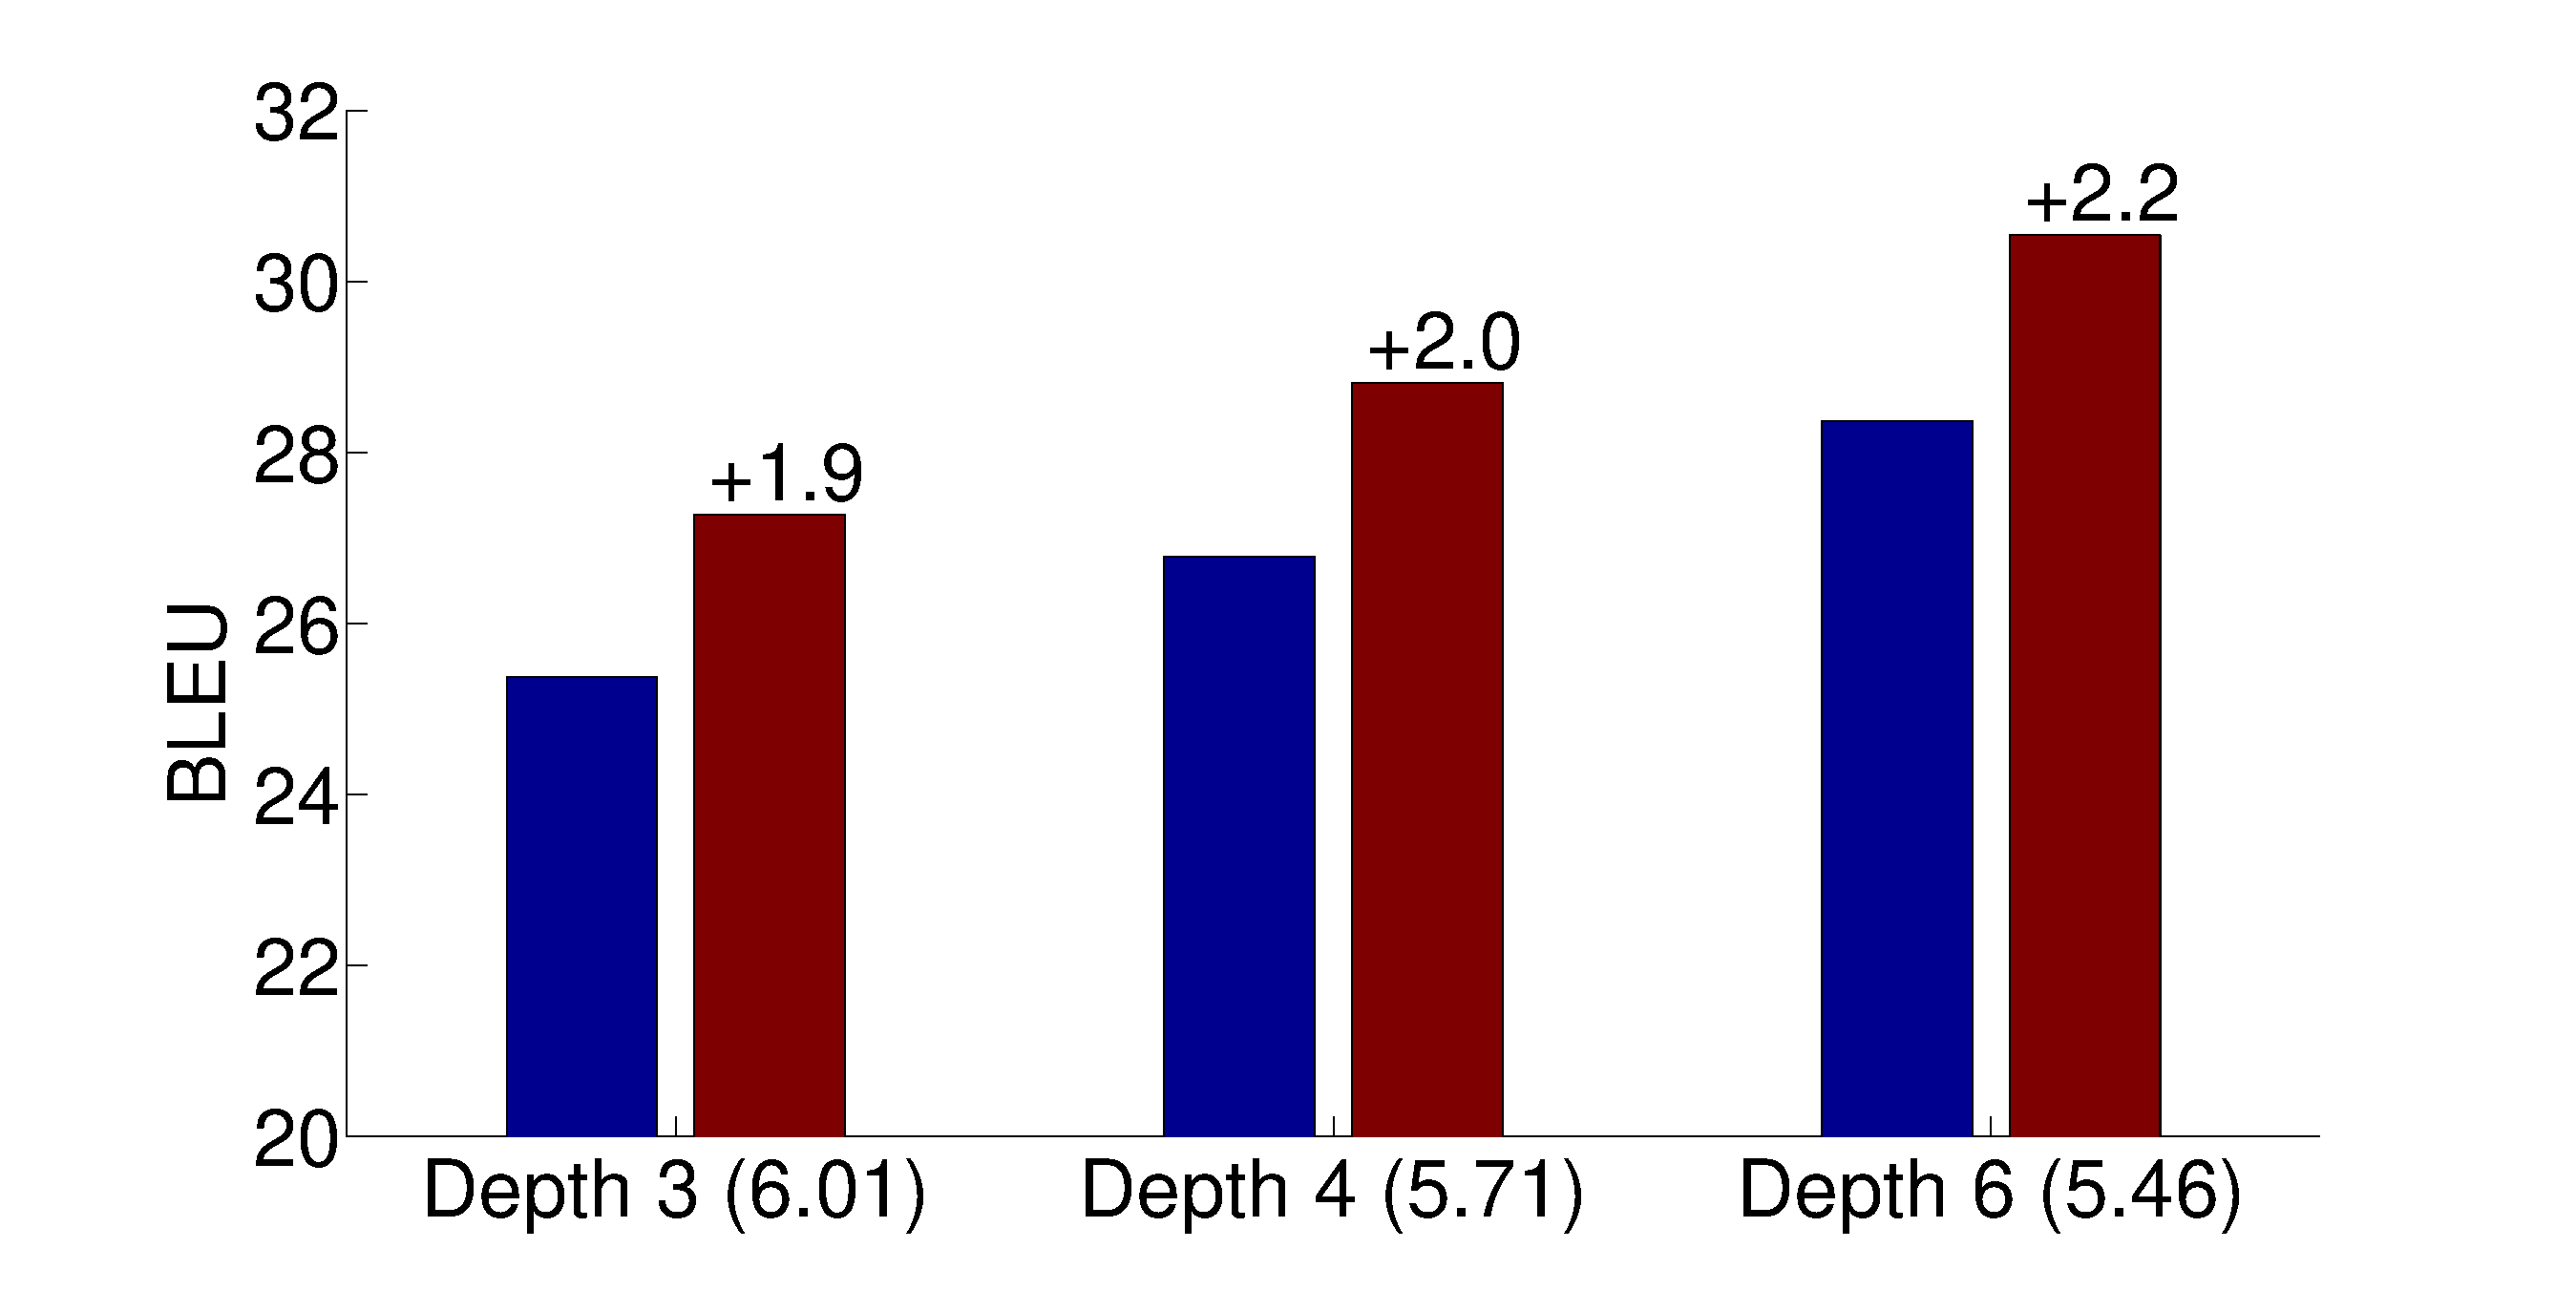
\includegraphics[width=0.7\textwidth, clip=true, trim= 0 0 0 0]{img/3-depth} % , angle=-90
\caption[Effect of depths]{{\bf Effect of depths} -- BLEU scores achieved by {\it PosUnk} models of various depths (3, 4, and 6) before and after the rare word translation. 
 Notice that the PosUnk model is more useful on more accurate models. }
\label{f:depth}
\end{figure}

{\bf Perplexity and BLEU} -- Lastly, I find it interesting to observe a strong correlation 
between the perplexity (my training objective) and the translation quality as measured by BLEU. 
Figure~\ref{f:cor} shows the performance of a 4-layer LSTM, in which I compute both perplexity and 
BLEU scores at different points during training. I find that on average, a reduction of 0.5 perplexity 
gives us roughly 1.0 BLEU point improvement.
\begin{figure}[tbh!]
\centering
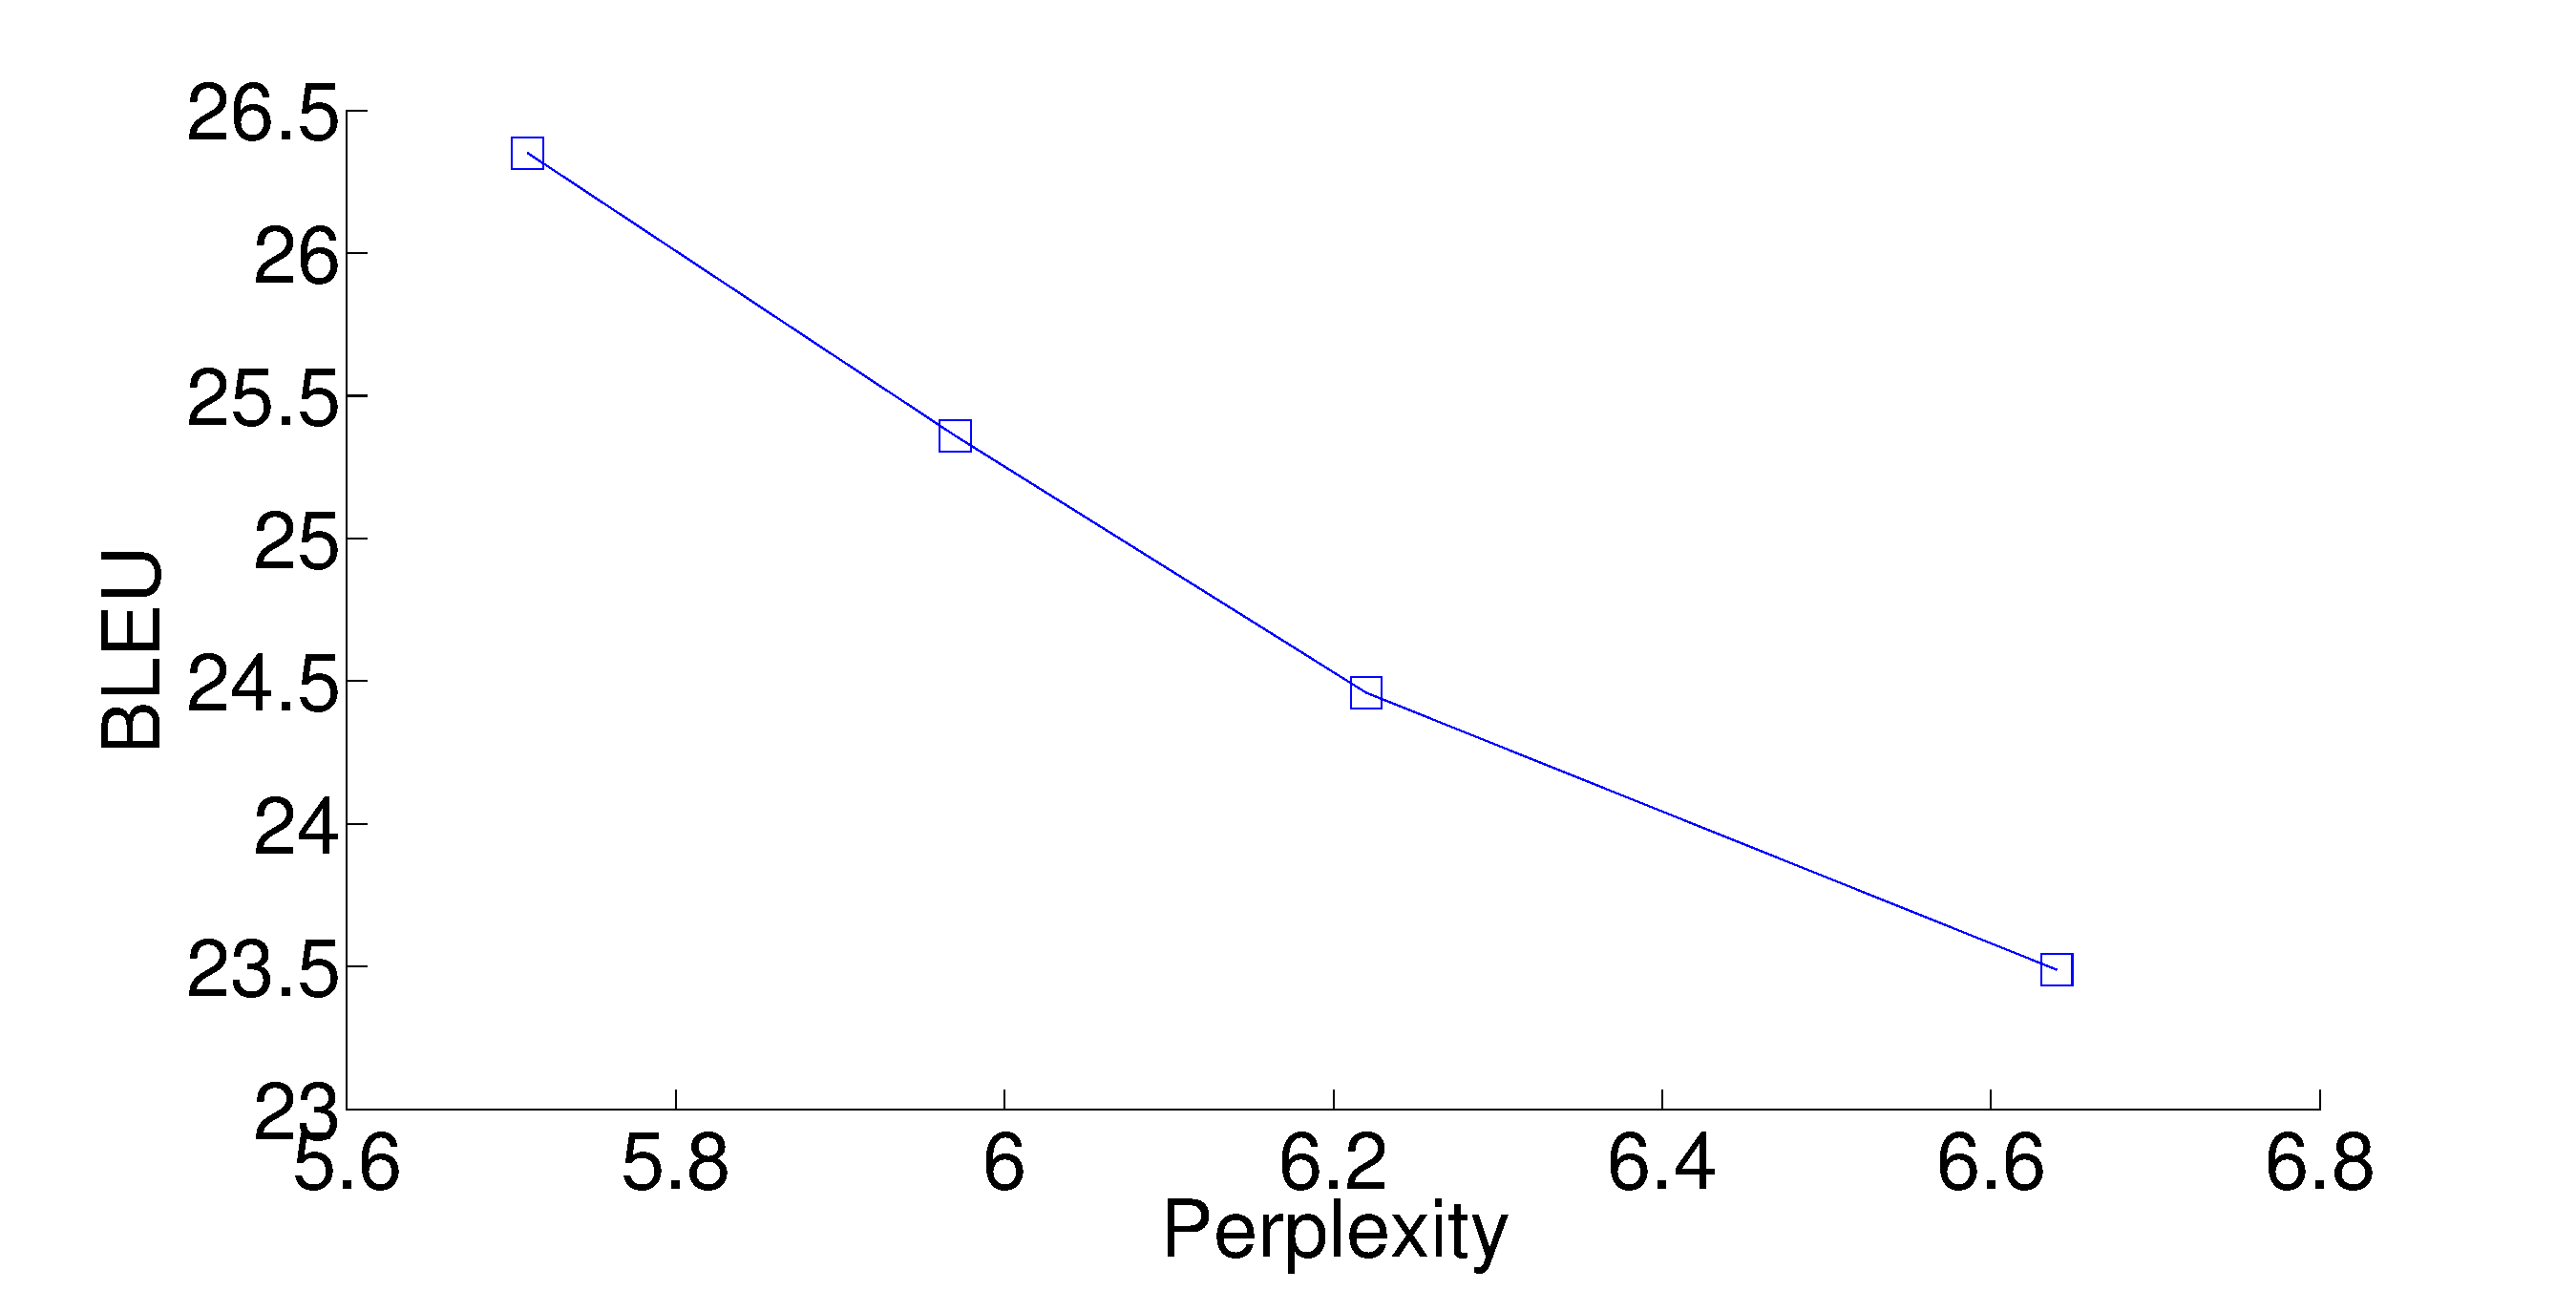
\includegraphics[width=0.7\textwidth, clip=true, trim= 0 0 0 0]{img/3-cor} % , angle=-90
\caption[Perplexity vs. BLEU]{{\bf Perplexity vs. BLEU} -- I show the correlation by evaluating an LSTM model with 4 layers at various stages of training. 
} 
\label{f:cor}
\end{figure}


\subsection{Sample Translations}
I present three sample translations of my best system
(with \bestbleuunk{} BLEU) in Table~\ref{t:sample}. In my  first example,
the model translates all the
unknown words correctly: {\it 2600}, {\it orthop{\'e}diques}, and {\it
cataracte}. It is interesting to observe that the model can accurately predict
an alignment of distances of 5 and 6 words. The second
example highlights the fact that my model can translate long
sentences reasonably well and that it was able to
correctly translate the unknown word for {\it JPMorgan} at the very far end of
the source sentence. Lastly, my examples also reveal several
penalties incurred by my model: (a) incorrect entries in the word dictionary, as with {\it n\'{e}gociateur} vs. {\it trader} in the second example, 
%identical meaning with different words, as with {\it n\'{e}gociateur} vs. {\it trader} in the second example, 
and (b) incorrect alignment prediction, such as when 
 \unkpostext{3} is incorrectly aligned
with the source word {\it was} and not with {\it abandoning}, which resulted in an
incorrect translation in the third sentence.

\begin{table*}[tbh!]
\centering
\resizebox{13.5cm}{!}{
\begin{tabular}{c|p{12cm}}
\bf{} & \bf{Sentences}\\
  \hline
src & An additional {\it 2600} operations including {\it orthopedic} and {\it cataract} surgery will help clear a backlog .\\
  \hline
trans & En outre , \unkpos{1} op{\'e}rations suppl{\'e}mentaires , dont la chirurgie \unkpos{5} et la \unkpos{6} , permettront de r{\'e}sorber l' arri{\'e}r{\'e} .\\
  \hline
+unk & En outre , {\it 2600} op{\'e}rations suppl{\'e}mentaires , dont la chirurgie {\it orthop{\'e}diques} et la {\it cataracte} , permettront de r{\'e}sorber l' arri{\'e}r{\'e} .\\
  \hline
tgt & 2600 op{\'e}rations suppl{\'e}mentaires , notamment dans le domaine de la chirurgie orthop{\'e}dique et de la cataracte , aideront {\`a} rattraper le retard .\\
  \hline
  \hline
src & This {\it trader} , Richard {\it Usher} , left RBS in {\it 2010} and is understand to have be given leave from his current position as European head of forex spot trading at {\it JPMorgan} .\\
  \hline
trans & Ce \unkpos{0} , Richard \unkpos{0} , a quitt{\'e} \unkpos{1} en 2010 et a compris qu' il est autoris{\'e} {\`a} quitter son poste actuel en tant que leader europ{\'e}en du march{\'e} des points de vente au \unkpos{5} .\\
  \hline
+unk & Ce {\it n\'{e}gociateur} , Richard {\it Usher} , a quitt{\'e} RBS en {\it 2010} et a compris qu' il est autoris{\'e} {\`a} quitter son poste actuel en tant que leader europ{\'e}en du march{\'e} des points de vente au {\it JPMorgan} .\\
  \hline
tgt & Ce trader , Richard Usher , a quitt{\'e} RBS en 2010 et aurait {\'e}t{\'e} mis suspendu de son poste de responsable europ{\'e}en du trading au comptant pour les devises chez JPMorgan \\
  \hline
  \hline
src & But concerns have grown after Mr {\it Mazanga} was quoted as saying {\it Renamo} {\it was} abandoning the 1992 peace accord .\\
  \hline
trans & Mais les inqui{\'e}tudes se sont accrues apr{\`e}s que M. \unkpos{3} a d{\'e}clar{\'e} que la \unkpos{3} \unkpos{3} l' accord de paix de 1992 .\\
  \hline
+unk & Mais les inqui{\'e}tudes se sont accrues apr{\`e}s que M. {\it Mazanga} a d{\'e}clar{\'e} que la {\it Renamo} {\it {\'e}tait} l' accord de paix de 1992 .\\
  \hline
tgt & Mais l' inqui{\'e}tude a grandi apr{\`e}s que M. Mazanga a d{\'e}clar{\'e} que la Renamo abandonnait l' accord de paix de 1992 .\\
\end{tabular}
}
\caption[Sample translations]{{\bf Sample translations} -- the table shows the source ({\it src}) and the translations of my best model before ({\it trans}) and after ({\it +unk}) unknown word translations. I also show the human translations ({\it tgt}) and italicize words that are involved in the unknown word translation process.}
\label{t:sample}
\end{table*}


\section{Conclusion}
\label{sec:conclude}
I have shown that a simple alignment-based technique can mitigate and even
overcome one of the main weaknesses of current NMT systems, which is
their inability to translate words that are not in their vocabulary.  
A key advantage of my technique is the fact that it is applicable to any NMT system and not
only to the deep LSTM model of \newcite{sutskever14}. At the time of this work, in 2014-2015, a technique
like mine is likely necessary if an NMT system is to achieve state-of-the-art performance
on machine translation.

I have demonstrated empirically that on the WMT'14 English-French translation task, my technique yields a 
consistent and substantial improvement of up to \bestunkimp{} BLEU points over various NMT systems of different architectures. 
Most importantly, with \bestbleuunk{} BLEU points, I have established the first NMT system that outperformed 
the best MT system on a WMT'14 contest dataset.

I will now switch gear to address a different problem in NMT,
that is the difficulty in translating long sentences. However, I will return back
to the topic of rare and unknown words in Chapter 5 to present an even better treatment to that problem.




\chapter{Attention Mechanisms}
\label{c:attention}
While I have demonstrated in the previous chapter that Neural Machine Translation (NMT) can achieve state-of-the-art performance in
large-scale translation tasks such as from English to French, it is still challenging for NMT to handle long sentences as observed by \newcite{bog15}.
One effective way to address such problem is through the attention mechanism, which has gained popularity recently in
training neural networks, allowing models to learn alignments between different
modalities, e.g., between image objects and agent actions in the dynamic control
problem \cite{mnih14}, between speech frames and text in the speech recognition
task \cite{jan14},  or between visual features of a picture and its text
description in the image caption generation task \cite{xu15}. In the context of
NMT, \newcite{bog15} has successfully applied such attentional mechanism to
jointly translate and align words. To the best of my knowledge during the time of this work, there has not
been any other work exploring the use of attention-based architectures for NMT.

\begin{figure}
\centering
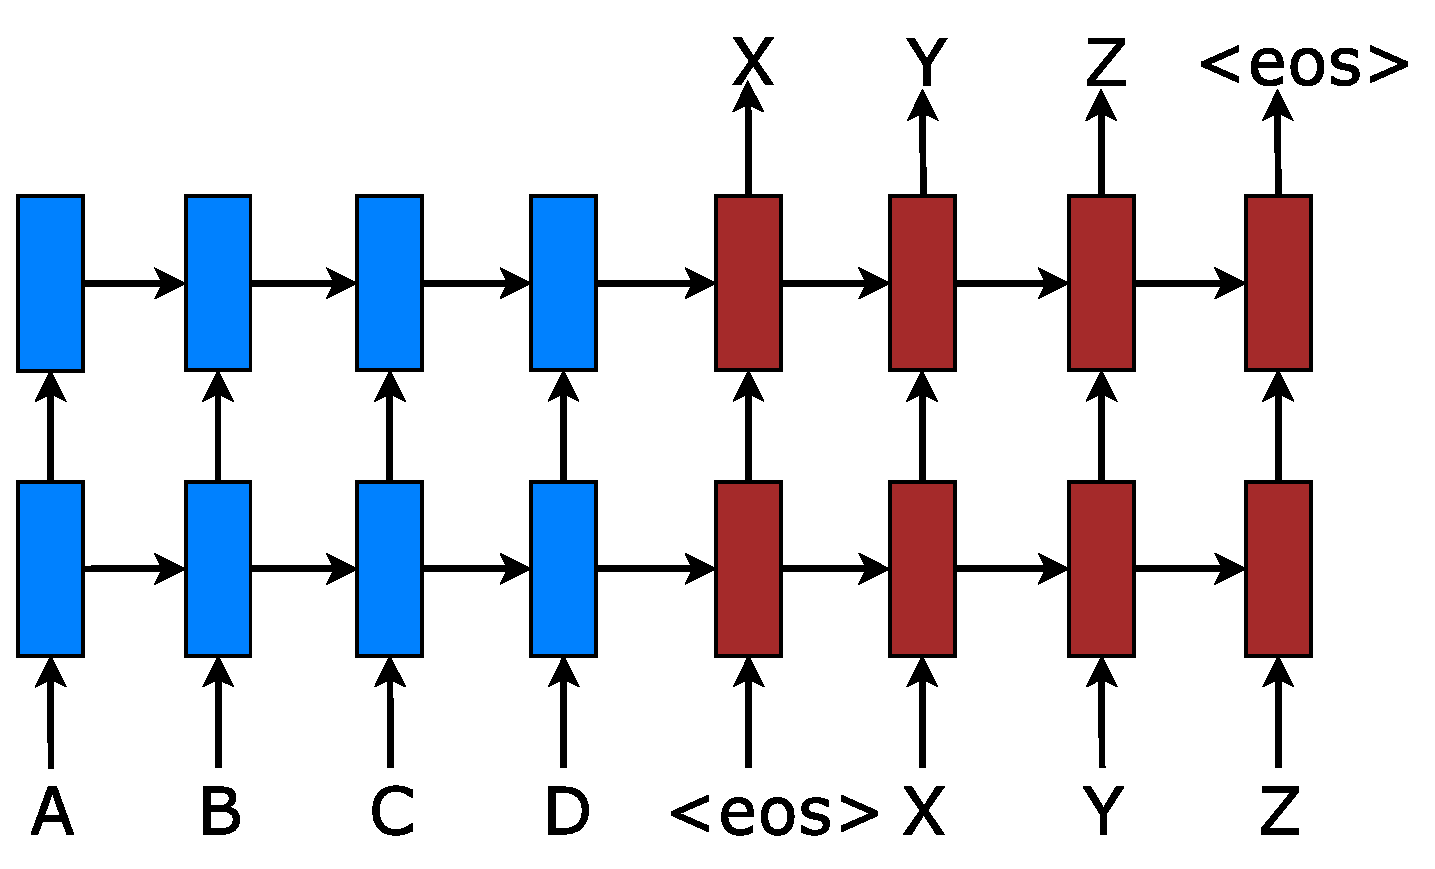
\includegraphics[width=0.45\textwidth, clip=true, trim= 0 0 0 0]{img/4-lstm} % , angle=-90
\caption[Neural machine translation]{{\bf Neural machine translation} -- a stacking recurrent architecture for translating a source sequence \texttt{A B C D} into a target sequence \texttt{X Y Z}. Here, \eos{} marks the end of a sentence.
} 
\label{f:lstm}
\end{figure}

In this work, I design, with simplicity and effectiveness in mind, two novel
types of attention-based models: a {\it global} approach in which all source
words are attended and a {\it local} one whereby only a subset of source words
are considered at a time. The former approach resembles the model of
\cite{bog15} but is simpler architecturally. The latter can be viewed as an
interesting blend between the {\it hard} and {\it soft} attention models
proposed in \cite{xu15}: it is computationally less expensive than the
global model or the soft attention; at the same time, unlike the hard attention,
the local attention is
differentiable almost everywhere, making it easier to implement and
train.\footnote{There is a recent work by \newcite{draw15}, which is very
similar to my local attention and applied to the image generation task.
However, as I detail later, my model is much simpler and can achieve good performance for NMT.} Besides, I also examine various
alignment functions for my attention-based models.

Following \cite{sutskever14,luong15}, I use the stacking LSTM architecture for our NMT systems, as illustrated in Figure~\ref{f:lstm}, together with the LSTM unit defined in \cite{zaremba14}.
The experimental results demonstrate that both of my approaches are
effective in the WMT translation tasks between English and German in  both
directions. My attentional models yield a boost of up to \attngain{} BLEU over
non-attentional systems which already incorporate known techniques such as
dropout. For English to German translation, I achieve new state-of-the-art
(SOTA)
results for both WMT'14 and WMT'15, outperforming previous SOTA systems, backed by
NMT models and $n$-gram LM rerankers, by more than 1.0 BLEU. I conduct
extensive analysis to evaluate my models in terms of learning, the ability to
handle long sentences, choices of attentional architectures, alignment quality, and translation
outputs. 

\section{Attention-based Models}
\label{sec:attn}
Unlike the basic NMT systems \cite{kal13,sutskever14,cho14,luong15}, in which the source representation is only used once to initialize the decoder hidden state, the idea of the {\it attention mechanism} explored in \cite{bog15,jean15} and this work is to provide a ``random access memory'' of source hidden states which one can constantly refer to as translation progresses.
The various attention-based models proposed in this work can be classified into two broad categories, {\it global} and {\it local}. These classes differ in terms of whether the ``attention'' is placed on all source positions or on only a few source positions. I illustrate these two model types in Figure~\ref{f:soft_attn} and \ref{f:hard_attn} respectively.

Common to these two types of models is the fact that at each time step $t$ in the decoding phase, both approaches first take as input the hidden state $\hi$ at the top layer of a stacking LSTM. The goal is then to derive a context vector $\co$ that captures relevant source-side information to help predict the current target word $\tgt{t}$. While these models differ in how the context vector $\co$ is derived, they share the same subsequent steps. 
Specifically, given the target hidden state $\hi$ and the source-side context vector $\co$, I employ a simple concatenation layer to combine the information from both vectors to produce an attentional hidden state as follows:
\begin{equation}
\hs = \tanh(\W{c}[\co; \hi])
\label{e:hs}
\end{equation} 

The attentional vector $\hs$ is then fed through the softmax layer to produce the predictive distribution formulated as:
\begin{equation}
p(\tgt{t}|\tgt{<t},\src{}) = \softmax(\W{s}\hs)
\label{e:predict}
\end{equation} 

I now detail how each model type computes the source-side context vector $\co$.

\subsection{Global Attention}
\label{subsec:global}
\begin{figure}
\centering
%\psgrid
\rput(7.1,6.6){$\tgt{t}$}
\rput(2.7,4){$\co$}
\rput(5,3.1){$\al$}
\rput(7.9,1.9){$\hi$}
\rput(7.9,6){$\hs$}
\rput(0.3,2.3){$\his$}
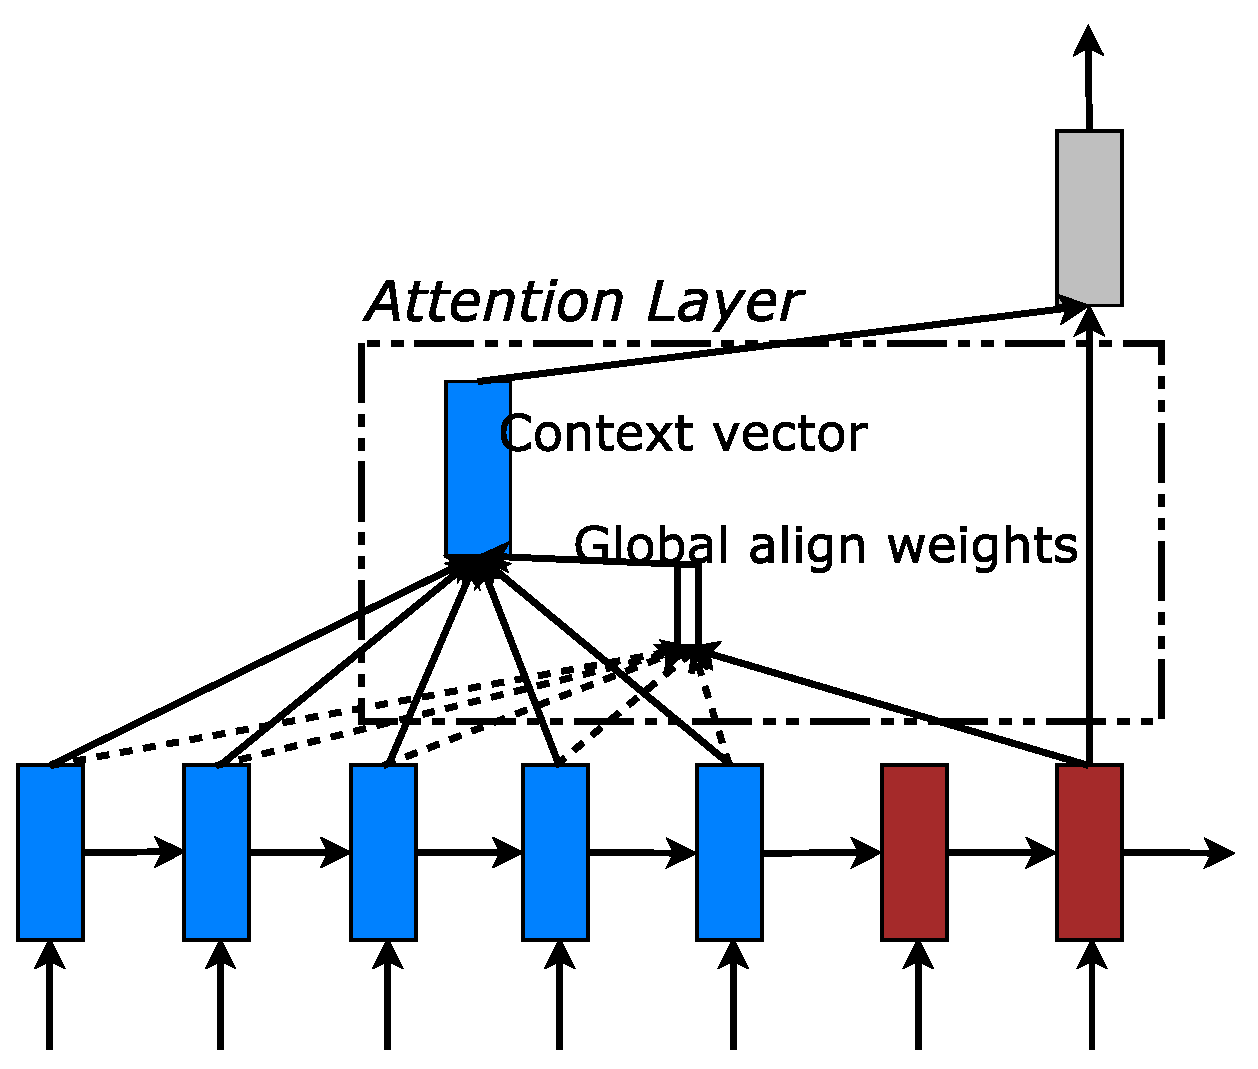
\includegraphics[width=0.55\textwidth, clip=true, trim= 0 0 0 0]{img/4-attn_soft} % , angle=-90
\caption[Global attentional model]{{\bf Global attentional model} -- at each time step $t$, the model infers a {\it variable-length} alignment weight vector $\al$ based on the current target state $\hi$ and all source states $\his$. A global context vector $\co$ is then computed as the weighted average, according to $\al$, over all the source states. 
} 
\label{f:soft_attn}
\end{figure}

The idea of a global attentional model is to consider all the hidden states of
the encoder when deriving the context vector $c_t$. In this model type, a
variable-length alignment vector $\al$, whose size equals the number of time
steps on the source side, is derived by comparing the current target hidden
state $\hi$ with each source hidden state $\his$:
\begin{align}
\label{e:al}
\al(s)&=\alignf(\hi, \his) \\
&=\frac{\exp \open{\score(\hi, \his)}}{\sum_{s'} \exp \open{\score(\hi,
\MB{\bar{h}}_{s'})}} \notag
\end{align}
Here, $\score$ is referred to as a {\it content-based} function for which I consider three different
alternatives:
\begin{equation*}
\score(\hi, \his)\!=\!\begin{cases}
    \tp{\hi} \his & \mbox{{\it dot}}\\
    \tp{\hi} \MB{W_a} \his & \mbox{{\it general}} \\
    \tp{\MB{v}_a}\tanh\open{\MB{W_a} [\hi; \his]} & \mbox{{\it concat}}
\end{cases}
\end{equation*}

In addition, in our early attempts to build attention-based models, I used
a {\it location-based} function in which the alignment scores are
computed from solely the target hidden state $\hi$ as
follows:
\begin{equation}
\al = \softmax(\W{a}\hi) \mbox{ } \mbox{ } \mbox{ } \mbox{ } \mbox{ } \mbox{ } \mbox{ } \mbox{ } \mbox{ } \mbox{ } \mbox{ } \mbox{ } \mbox{ } \mbox{ } \mbox{ } \mbox{ } \mbox{{\it location}}
\label{e:location}
\end{equation}
Given the alignment vector as weights, the
context vector $c_t$ is computed as the  weighted average over all the source hidden states.\footnote{\eq{e:location} implies that
all alignment vectors $\al$ are of the same length. For short sentences, I only
use the top part of $\al$ and for long sentences, I ignore words near the end.}

\textit{Comparison to \cite{bog15}} --
% An example of such model is the work of \newcite{bog15}. 
While our global attention approach is similar in spirit to the model proposed
by \newcite{bog15}, there are several key differences which reflect how I have
both simplified and generalized from the original model. First, I simply use
hidden states at the top LSTM layers in both the encoder and decoder as
illustrated in Figure~\ref{f:soft_attn}. \newcite{bog15}, on the other hand,
use the concatenation of the forward and backward source 
hidden states in the bi-directional encoder and target hidden
states in their non-stacking uni-directional decoder. Second, our computation
path is simpler; I go from $\hi \rightarrow \al \rightarrow \co \rightarrow
\hs$ then make a prediction as detailed in \eq{e:hs}, \eq{e:predict}, and
Figure~\ref{f:soft_attn}. On the other hand, at any time $t$, \newcite{bog15} build from the previous hidden state $\hid{t-1} \rightarrow \al \rightarrow \co \rightarrow \hi$, which, in turn, goes through a deep-output and a maxout layer before making predictions.\footnote{I will refer to this difference again in Section~\ref{subsec:input}.} Lastly, \newcite{bog15} only experimented with one alignment function, the {\it concat} product; whereas I show later that the other alternatives are better.

\subsection{Local Attention}
\begin{figure}
\centering
%\psgrid
\rput(7.1,6.6){$\tgt{t}$}
\rput(2.7,4){$\co$}
\rput(3.8,2.9){$\al$}
\rput(7.9,1.9){$\hi$}
\rput(7.9,6){$\hs$}
\rput(6.5,3.4){$p_t$}
\rput(0.3,2.3){$\his$}
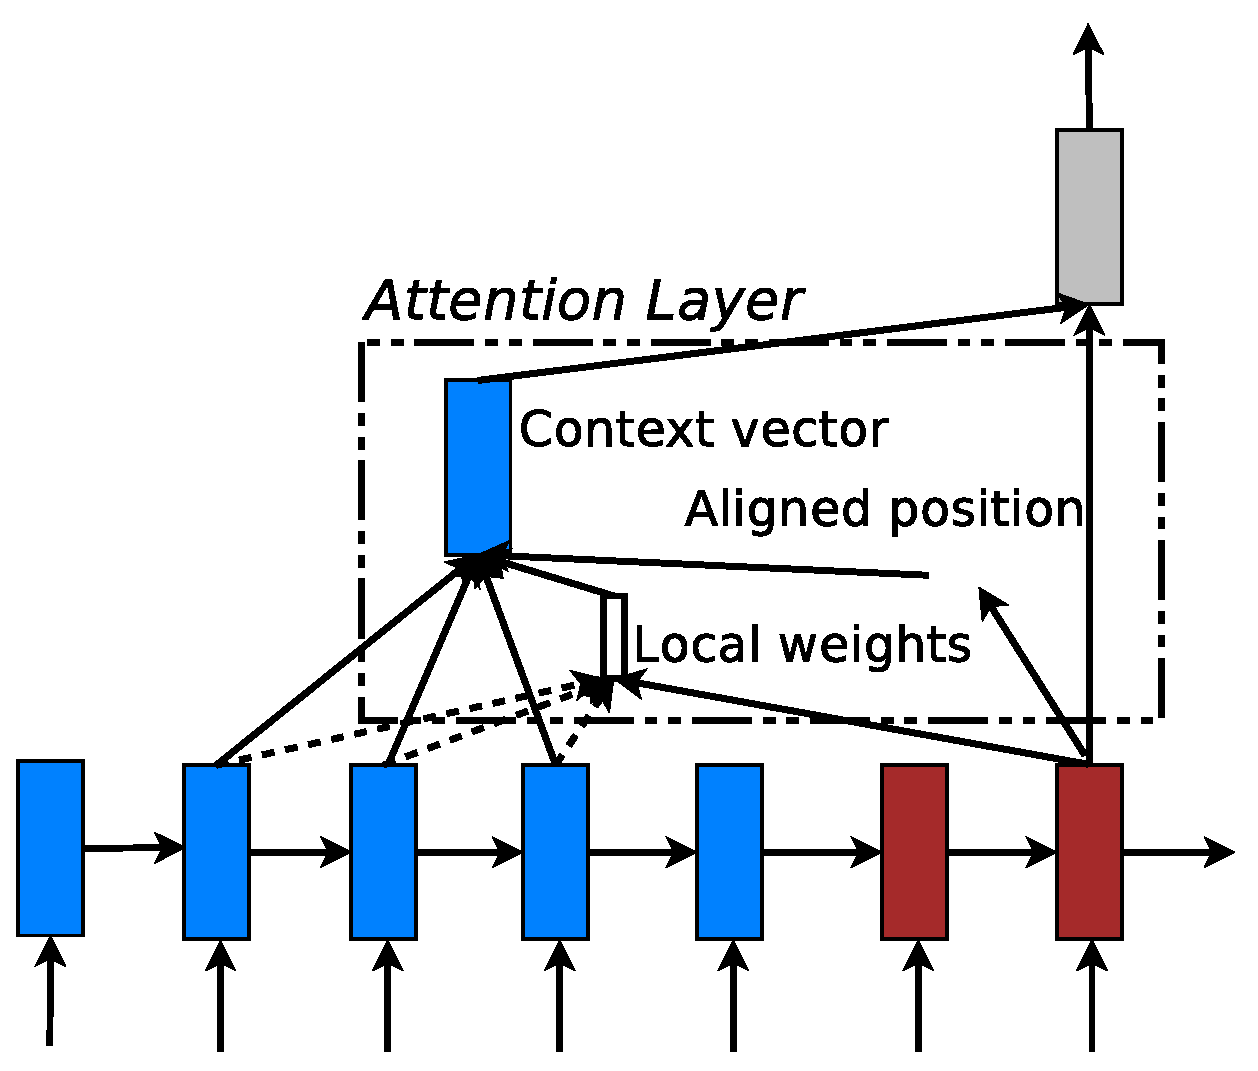
\includegraphics[width=0.55\textwidth, clip=true, trim= 0 0 0 0]{img/4-attn_hard} % , angle=-90
\caption[Local attention model]{{\bf Local attention model} -- the model first predicts a single
aligned position $p_t$ for the current target word. A window centered around the
source position $p_t$ is then used to compute a context vector $\co$, a weighted
average of the source hidden states in the window. The weights $\MB{\al}$ are
inferred from the current target state $\hi$ and those source states $\his$ in
the window.
%similar to the global attention model in Figure~\ref{f:soft_attn}, instead of producing a global alignment vector, 
} 
\label{f:hard_attn}
\end{figure}

The global attention has a drawback that it has to attend to all words on the
source side for each target word, which is expensive and can potentially render it impractical to
translate longer sequences, e.g., paragraphs or documents.
To address this deficiency, I propose a {\it local} attentional mechanism that
chooses to focus only on a small subset of the source positions per target word.

This model takes inspiration from the tradeoff between the {\it soft} and {\it
hard} attentional models proposed by \newcite{xu15} to tackle the image caption
generation task. In their work, soft attention refers to the global attention
approach in which weights are placed ``softly'' over all patches in the source
image. The hard attention, on the other hand, selects one patch
of the image to attend to at a time. While less expensive at inference time, the
hard attention model is non-differentiable and requires more complicated
techniques such as variance reduction or reinforcement learning to train.

My local attention mechanism selectively focuses on a small window of
context and is differentiable. This approach has an advantage of avoiding the expensive computation incurred in
the soft attention and at the same time, is easier to train than the hard
attention approach.
In concrete details, the model first generates an aligned position $p_t$ for each target word at time $t$. The
context vector $\co$ is then derived as a weighted average over the set of source hidden states within the window $[p_t-D, p_t+D]$; $D$ is
empirically selected.\footnote{If the window crosses the sentence boundaries, I
simply ignore the outside part and consider words in the window.} Unlike the global approach, the local alignment vector $\al$ is now fixed-dimensional, i.e., $\inR{2D+1}$. %is generated in the same manner as the global attentional model except that its dimension is $(2D+1)$.
I consider two variants of the model as below.

\textit{Monotonic} alignment ({\bf \localm{}}) -- I simply set % 
$\pt\!=\!t$ assuming that source and target sequences are roughly
monotonically aligned. The alignment vector $\al$ is defined according to
\eq{e:al}.\footnote{{\it local-m} is the same as
the global model except that the vector $\al$ is
fixed-length and shorter.} % This model is differentiable.

\textit{Predictive} alignment ({\bf \localp{}}) --  %
instead of assuming monotonic alignments, our model predicts an aligned position as follows:
\begin{equation}
\pt = S \cdot \sigmoid(\tp{\MB{v}_p}\tanh(\W{p}\hi)),
\label{e:p}
\end{equation}
$\W{p}$ and $\MB{v}_p$ are the model parameters which will be learned
to predict positions. $S$ is the source sentence length. As a result of $\sigmoid$, $\pt
\in [0, S]$. To favor alignment points near $\pt$, I place a Gaussian distribution centered around $\pt$ . Specifically, our alignment weights are now
defined as:
\begin{equation}
\al(s) = \alignf(\hi, \his) \exp \open{-\frac{(s-\pt)^2}{2\sigma^2}} 
\label{e:align_p}
\end{equation}
I use the same $\alignf$ function as in
\eq{e:al} and the standard deviation is empirically set as
$\sigma\!=\!\frac{D}{2}$. Note that $\pt$ is a {\it real} number; whereas $s$
is an {\it integer} within the window centered at $\pt$.\footnote{{\it local-p} is similar to the
local-m model except that I dynamically
compute $\pt$ and use a truncated Gaussian distribution to modify the original alignment
weights $\alignf(\hi, \his)$ as shown in \eq{e:align_p}. By utilizing $\pt$
to derive $\al$, I can compute backprop gradients for $\W{p}$ and $\MB{v}_p$.
This model is differentiable almost everywhere.} 

\textit{Comparison to \cite{draw15}} --
they have proposed a {\it selective attention} mechanism, very
similar to our local attention, for the image generation task. Their approach 
allows the model to select an image patch of varying location and zoom. I,
instead, use the same ``zoom'' for all target positions, which greatly
simplifies the formulation and still achieves good
performance.

\subsection{Input-feeding Approach}
\label{subsec:input}
In our proposed global and local approaches, the attentional decisions are made
independently, which is suboptimal. Whereas, in standard MT, a {\it coverage}
set is often maintained during the translation process to keep track of which
source words have been translated. Likewise, in attentional NMTs, alignment
decisions should be made jointly taking into account past alignment information.
To address that, I propose an {\it input-feeding} approach in which attentional
vectors $\hs$ are concatenated with inputs at the next time steps as illustrated in
Figure~\ref{f:input}.\footnote{If $n$ is the number of LSTM cells, the
input size of the first LSTM layer is $2n$; those of subsequent
layers are $n$.} The effects of having such connections are two-fold:
(a) I hope to make the model fully aware of previous alignment choices and (b)
I create a very deep network spanning both horizontally and vertically.

\begin{figure}
\centering
%\psgrid
\rput(3.5,6){$\hs$}
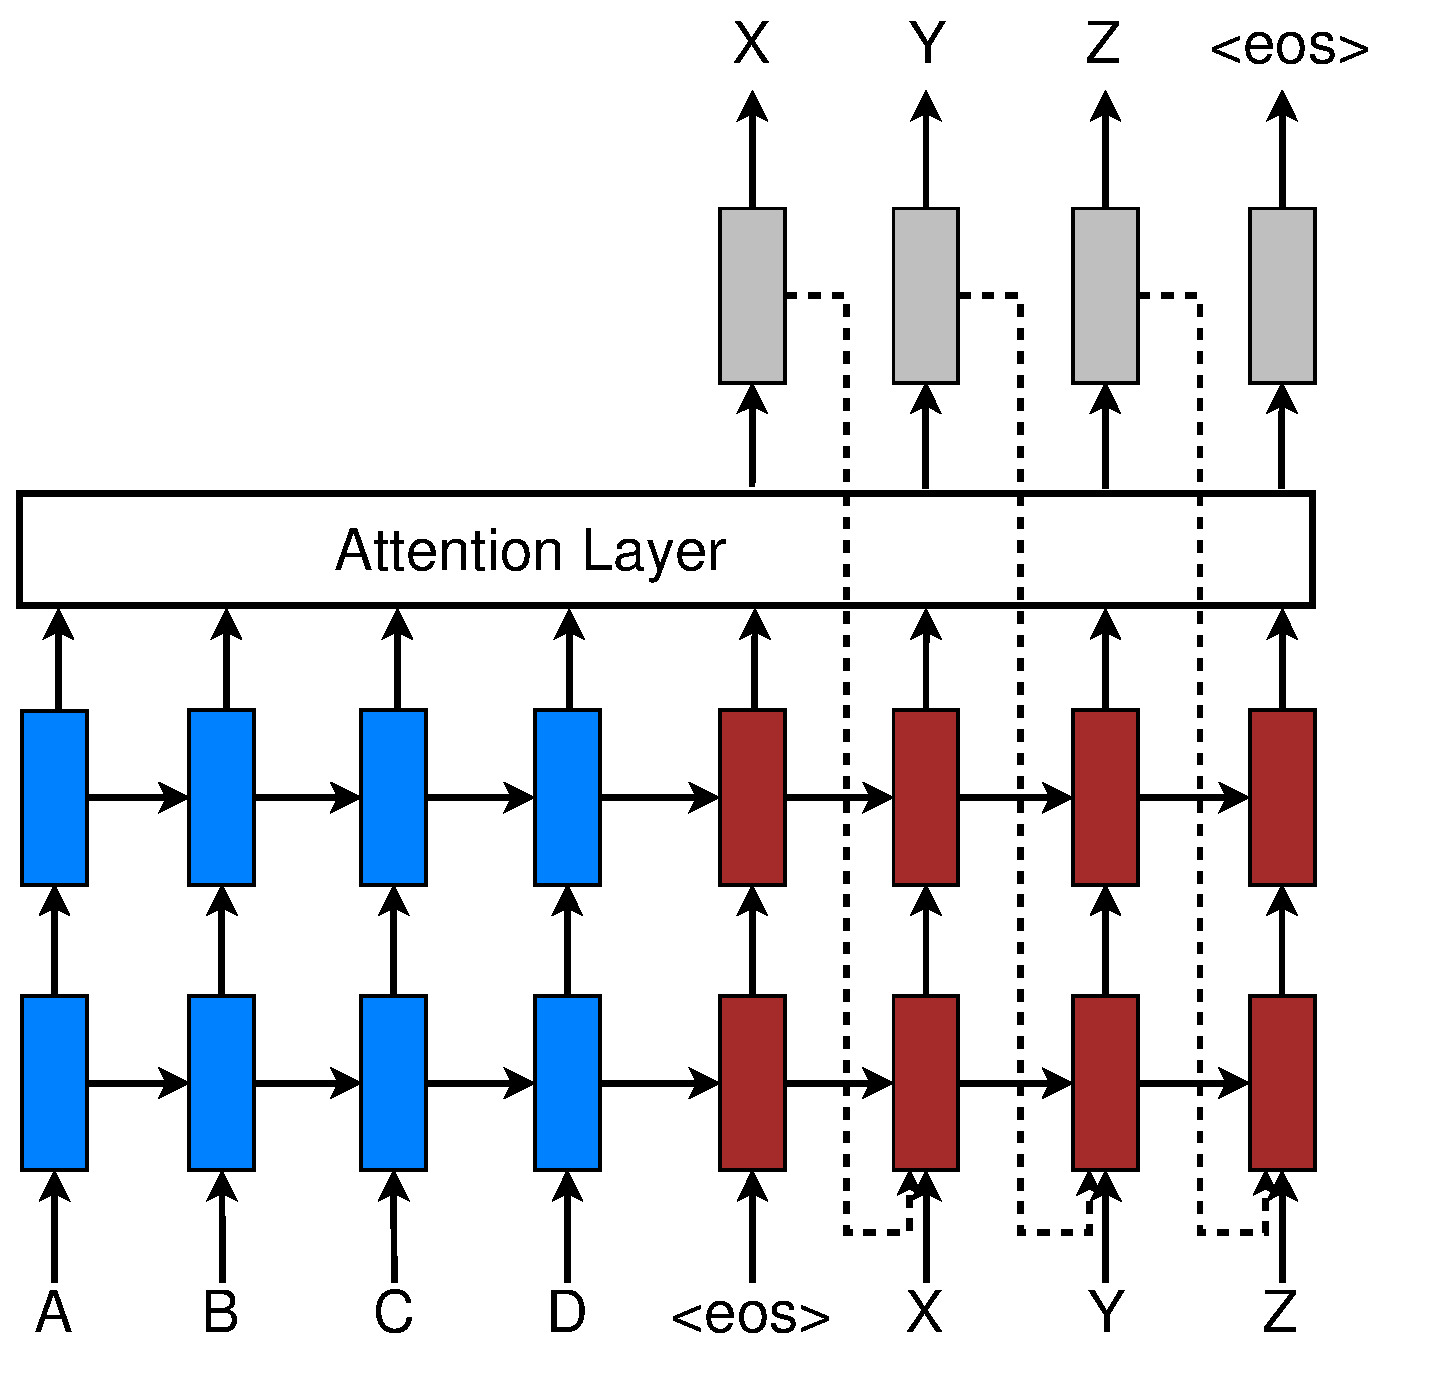
\includegraphics[width=0.5\textwidth, clip=true, trim= 0 0 0 0]{img/4-attn_input} % , angle=-90
\caption[Input-feeding approach]{{\bf Input-feeding approach} -- Attentional vectors $\hs$ are fed as inputs to the next time steps to inform the model about past alignment decisions.
} 
\label{f:input}
\end{figure}


{\it Comparison to other work} -- \newcite{bog15}
use context vectors, similar to
our $\co$, in building subsequent hidden states, which can also 
achieve the ``coverage'' effect. However, there has not been any analysis of 
whether such connections are useful as done in this work. Also,
our approach is more general; as illustrated in Figure~\ref{f:input}, it can be
applied to general stacking recurrent architectures, including non-attentional
models.

\newcite{xu15} propose a {\it doubly attentional} approach with an
additional constraint added to the training objective to make sure the model
pays equal attention to all parts of the image during the caption generation process. Such a constraint can also be useful to capture the coverage set effect in NMT that I mentioned earlier. However, I chose to use the input-feeding approach since it provides flexibility for the model to decide on any attentional constraints it deems suitable.

\section{Experiments}
\label{sec:exp}
I evaluate the effectiveness of my models on the WMT translation tasks between
English and German in both directions. newstest2013 (3000 sentences) is used as
a development set to select my hyperparameters. Translation performances are
reported in case-sensitive BLEU \cite{Papineni02bleu} on newstest2014 (2737 sentences) and
newstest2015 (2169 sentences). Following \cite{luong15}, I report
translation quality using two types of BLEU: (a) {\it
tokenized}\footnote{All texts are tokenized with \texttt{tokenizer.perl} and BLEU
scores are computed with \texttt{multi-bleu.perl}.} BLEU to be comparable with
existing NMT work and (b) {\it NIST}\footnote{With the \texttt{mteval-v13a}
script as per WMT guideline.} BLEU to be comparable
with WMT results.

\begin{table*}[tbh!]
\centering
\resizebox{15cm}{!}{
\begin{tabular}{l|r|c}
\bf{System} & \bf{Ppl} & \bf{BLEU}\\
  \hline
Winning WMT'14 system -- {\it phrase-based + large LM} \cite{buck14} &  & 20.7\\
  \hline
\multicolumn{3}{l}{{\it Existing NMT systems}}\\
  \hline
RNNsearch \cite{jean15} &  & 16.5\\
RNNsearch + unk replace \cite{jean15} &  & 19.0\\
RNNsearch + unk replace + large vocab + {\it ensemble} 8 models \cite{jean15} &  & {\bf 21.6}\\
  \hline
\multicolumn{3}{l}{{\it My NMT systems}}\\
  \hline
Base & 10.6 & 11.3\\
Base + reverse & 9.9 & 12.6 ({\it +1.3})\\
Base + reverse + dropout & 8.1 & 14.0 ({\it +1.4})\\
  \hdashline
Base + reverse + dropout + global attention ({\it location}) & 7.3 & 16.8 ({\it +2.8}) \\
Base + reverse + dropout + global attention ({\it location}) + feed input & 6.4
& 18.1 ({\it +1.3}) \\
  \hdashline
Base + reverse + dropout + local-p attention ({\it general}) + feed input
& \multirow{ 2}{*}{5.9} & 19.0 ({\it +0.9}) \\
Base + reverse + dropout + local-p attention ({\it general}) + feed input + unk replace
&  & 20.9 ({\it +1.9}) \\
  \hdashline
{\it Ensemble} 8 models + unk replace &  & {\bf 23.0 ({\it +2.1})} \\
\end{tabular}
}
\caption[WMT'14 English-German results]{{\bf WMT'14 English-German results} -- shown are
the perplexities (ppl) and the {\it tokenized} BLEU scores of various systems on newstest2014. I highlight the {\bf
best} system in bold and give {\it progressive} improvements in italic between
consecutive systems. {\it local-p} referes to the local attention with 
predictive alignments. I indicate for each attention model the
alignment score function used in parentheses. 
}
\label{t:ende}
\end{table*}


\subsection{Training Details}
All my models are trained on the WMT'14 training data consisting of 4.5M
sentences pairs (116M English words, 110M German words). Similar to \cite{jean15}, I limit my vocabularies to be the top 50K most frequent words for both languages. Words not in these shortlisted vocabularies are converted into a universal token \unk{}. 

When training my NMT systems, following \cite{bog15,jean15}, I filter out
sentence pairs whose lengths exceed 50 words and shuffle mini-batches as I
proceed. My stacking LSTM models have 4 layers, each with 1000 cells, and
1000-dimensional embeddings. I follow \cite{sutskever14,luong15} in training
NMT with similar settings: (a) my parameters are uniformly initialized in
$[-0.1, 0.1]$, (b) I train for 10 epochs using plain SGD, (c) a simple learning
rate schedule is employed -- I start with a learning rate of 1; after 5 epochs,
I begin to halve the learning rate every epoch, (d) my mini-batch size is 128,
and (e) the normalized gradient is rescaled whenever its norm exceeds 5.
Additionally, I also use dropout with probability $0.2$ for my LSTMs as suggested by
\cite{zaremba14}. For dropout models, I train for 12 epochs and start halving
the learning rate after 8 epochs. For local
attention models, I empirically set the window size $D=10$.

My code is implemented in MATLAB.
When running on a single GPU device Tesla K40, I achieve a speed of 1K {\it
target} words per second. It takes 7--10 days to completely train a model.

\subsection{English-German Results}
I compare my NMT systems in the English-German task with various other
systems. These include the winning system in WMT'14
\cite{buck14}, a phrase-based system whose language models were trained on a
huge monolingual text, the Common Crawl corpus. For end-to-end NMT systems, to the best of my knowledge, \cite{jean15} is the only work experimenting with this language pair and currently the SOTA system.
I only present results for some of my attention models and will later
analyze the rest in Section~\ref{sec:analysis}. 

\begin{sloppypar}
As shown in Table~\ref{t:ende}, I achieve progressive improvements when
(a) reversing the source sentence, +$1.3$ BLEU, as proposed in \cite{sutskever14}
and (b) using dropout, +$1.4$ BLEU. On top of that, (c) the global
attention approach gives a significant boost of +$2.8$ BLEU, making 
 my model slightly better than the base attentional system of
 \newcite{bog15} (row {\it RNNSearch}). When (d) using the {\it input-feeding}
approach, I seize another notable gain of +$1.3$ BLEU and outperform their
system. The local attention model with predictive alignments (row {\it \localp}) proves
to be even better, giving us a further improvement of +$0.9$ BLEU on top of the
global attention model. 
It is interesting to observe the trend previously reported in
\cite{luong15} that perplexity strongly correlates with translation quality.
In total, I achieve a significant gain of
\attngain{} BLEU points over the non-attentional baseline, which already includes
known techniques such as source reversing and dropout.
\end{sloppypar}

The unknown replacement technique proposed in \cite{luong15,jean15} yields another nice
gain of +$1.9$ BLEU, demonstrating that my attentional models
do learn useful alignments for unknown works. Finally, by ensembling 8 different
models of various settings, e.g., using different attention approaches, with
and without dropout etc., I was able to achieve a {\it new SOTA} result of
$\sotaold{}$
BLEU, outperforming the existing best system \cite{jean15} by +$1.4$ BLEU.

\begin{table}[tbh!]
\centering
%\resizebox{8cm}{!}{
\begin{tabular}{l|c}
\bf{System} & \bf{BLEU}\\
  \hline
Top -- {\it NMT + 5-gram rerank} (Montreal) & 24.9 \\
  \hline
My ensemble 8 models + unk replace & {\bf 25.9} \\
\end{tabular}
%}
\caption[WMT'15 English-German results]{{\bf WMT'15 English-German results} -- {\it NIST} BLEU scores of the
winning entry in WMT'15 and my best one on newstest2015.}
\label{t:wmt15ende}
\end{table}

{\it Latest results in WMT'15} -- despite the fact that my models were trained
on WMT'14 with slightly less data, I test them on newstest2015 to demonstrate
that they can generalize well to different test sets. As shown in Table~\ref{t:wmt15ende}, my best
system establishes a {\it new SOTA} performance of $\sotanew{}$ BLEU,
outperforming the existing best system backed by NMT and a 5-gram LM reranker
by +$1.0$
BLEU.

\subsection{German-English Results}
I carry out a similar set of experiments for the WMT'15 translation task from German
to English. 
While my systems have not yet matched the performance of the 
SOTA system, I nevertheless show the effectiveness of my
approaches with large and progressive gains in terms of BLEU as illustrated in
Table~\ref{t:deen}. 
The {\it attentional} mechanism gives us +$2.2$ BLEU gain and on top of that, I
obtain another boost of up to +$1.0$ BLEU from the {\it input-feeding} approach.
Using a better alignment function, the content-based {\it dot} product one,
together with {\it dropout} yields another gain of +$2.7$ BLEU. Lastly, when
applying the unknown word replacement technique, I seize an additional +$2.1$
BLEU, demonstrating the usefulness of attention in aligning rare words.
\begin{table}
\centering
%\resizebox{8cm}{!}{
\begin{tabular}{l|r|c}
\bf{System} & \bf{Ppl.} & \bf{BLEU}\\
  \hline
\multicolumn{3}{l}{{\it WMT'15 systems}}\\
  \hline
SOTA -- {\it phrase-based} (Edinburgh) &  & {\bf 29.2}\\ %\cite{freitag14}
NMT + 5-gram rerank (MILA) &  & 27.6\\ %\cite{freitag14}
  \hline
\multicolumn{3}{l}{{\it My NMT systems}}\\
  \hline
Base (reverse) & 14.3 & 16.9\\
  \hdashline
+ global ({\it location}) & 12.7 & 19.1 ({\it +2.2}) \\
+ global ({\it location}) + feed & 10.9 & 20.1 ({\it +1.0})\\
  \hdashline
+ global ({\it dot}) + drop + feed & \multirow{ 2}{*}{9.7} & 22.8 ({\it +2.7})\\
+ global ({\it dot}) + drop + feed + unk &  & 24.9 ({\it +2.1})\\
  %\hdashline
%{\it Ensemble} 4 models + unk &  & {\bf xx} ({\it +1.2})\\
\end{tabular}
%}
\caption[WMT'15 German-English results]{{\bf WMT'15 German-English results} -- 
performances of various systems (similar to 
Table~\ref{t:ende}). The {\it base} system already includes source reversing
on which I add {\it global} attention, {\it drop}out, input {\it feed}ing, and
{\it unk} replacement.}
\label{t:deen}
\end{table}

\section{Analysis}
\label{sec:analysis}
I conduct extensive analysis to better understand my models in terms
of learning, the ability to handle long sentences, 
choices of attentional architectures, and alignment quality. All results
reported here are on English-German newstest2014.

\subsection{Learning curves}
I compare models built on top of one another
as listed in Table~\ref{t:ende}. It is
pleasant to observe in Figure~\ref{f:learn} a clear separation between non-attentional and attentional
models. The input-feeding approach and the local attention
model also demonstrate their abilities in driving the test costs lower. The
non-attentional model with 
dropout (the blue + curve) learns slower than other non-dropout models, but
as time goes by, it becomes more robust in terms of minimizing test errors.
\begin{figure}
\centering
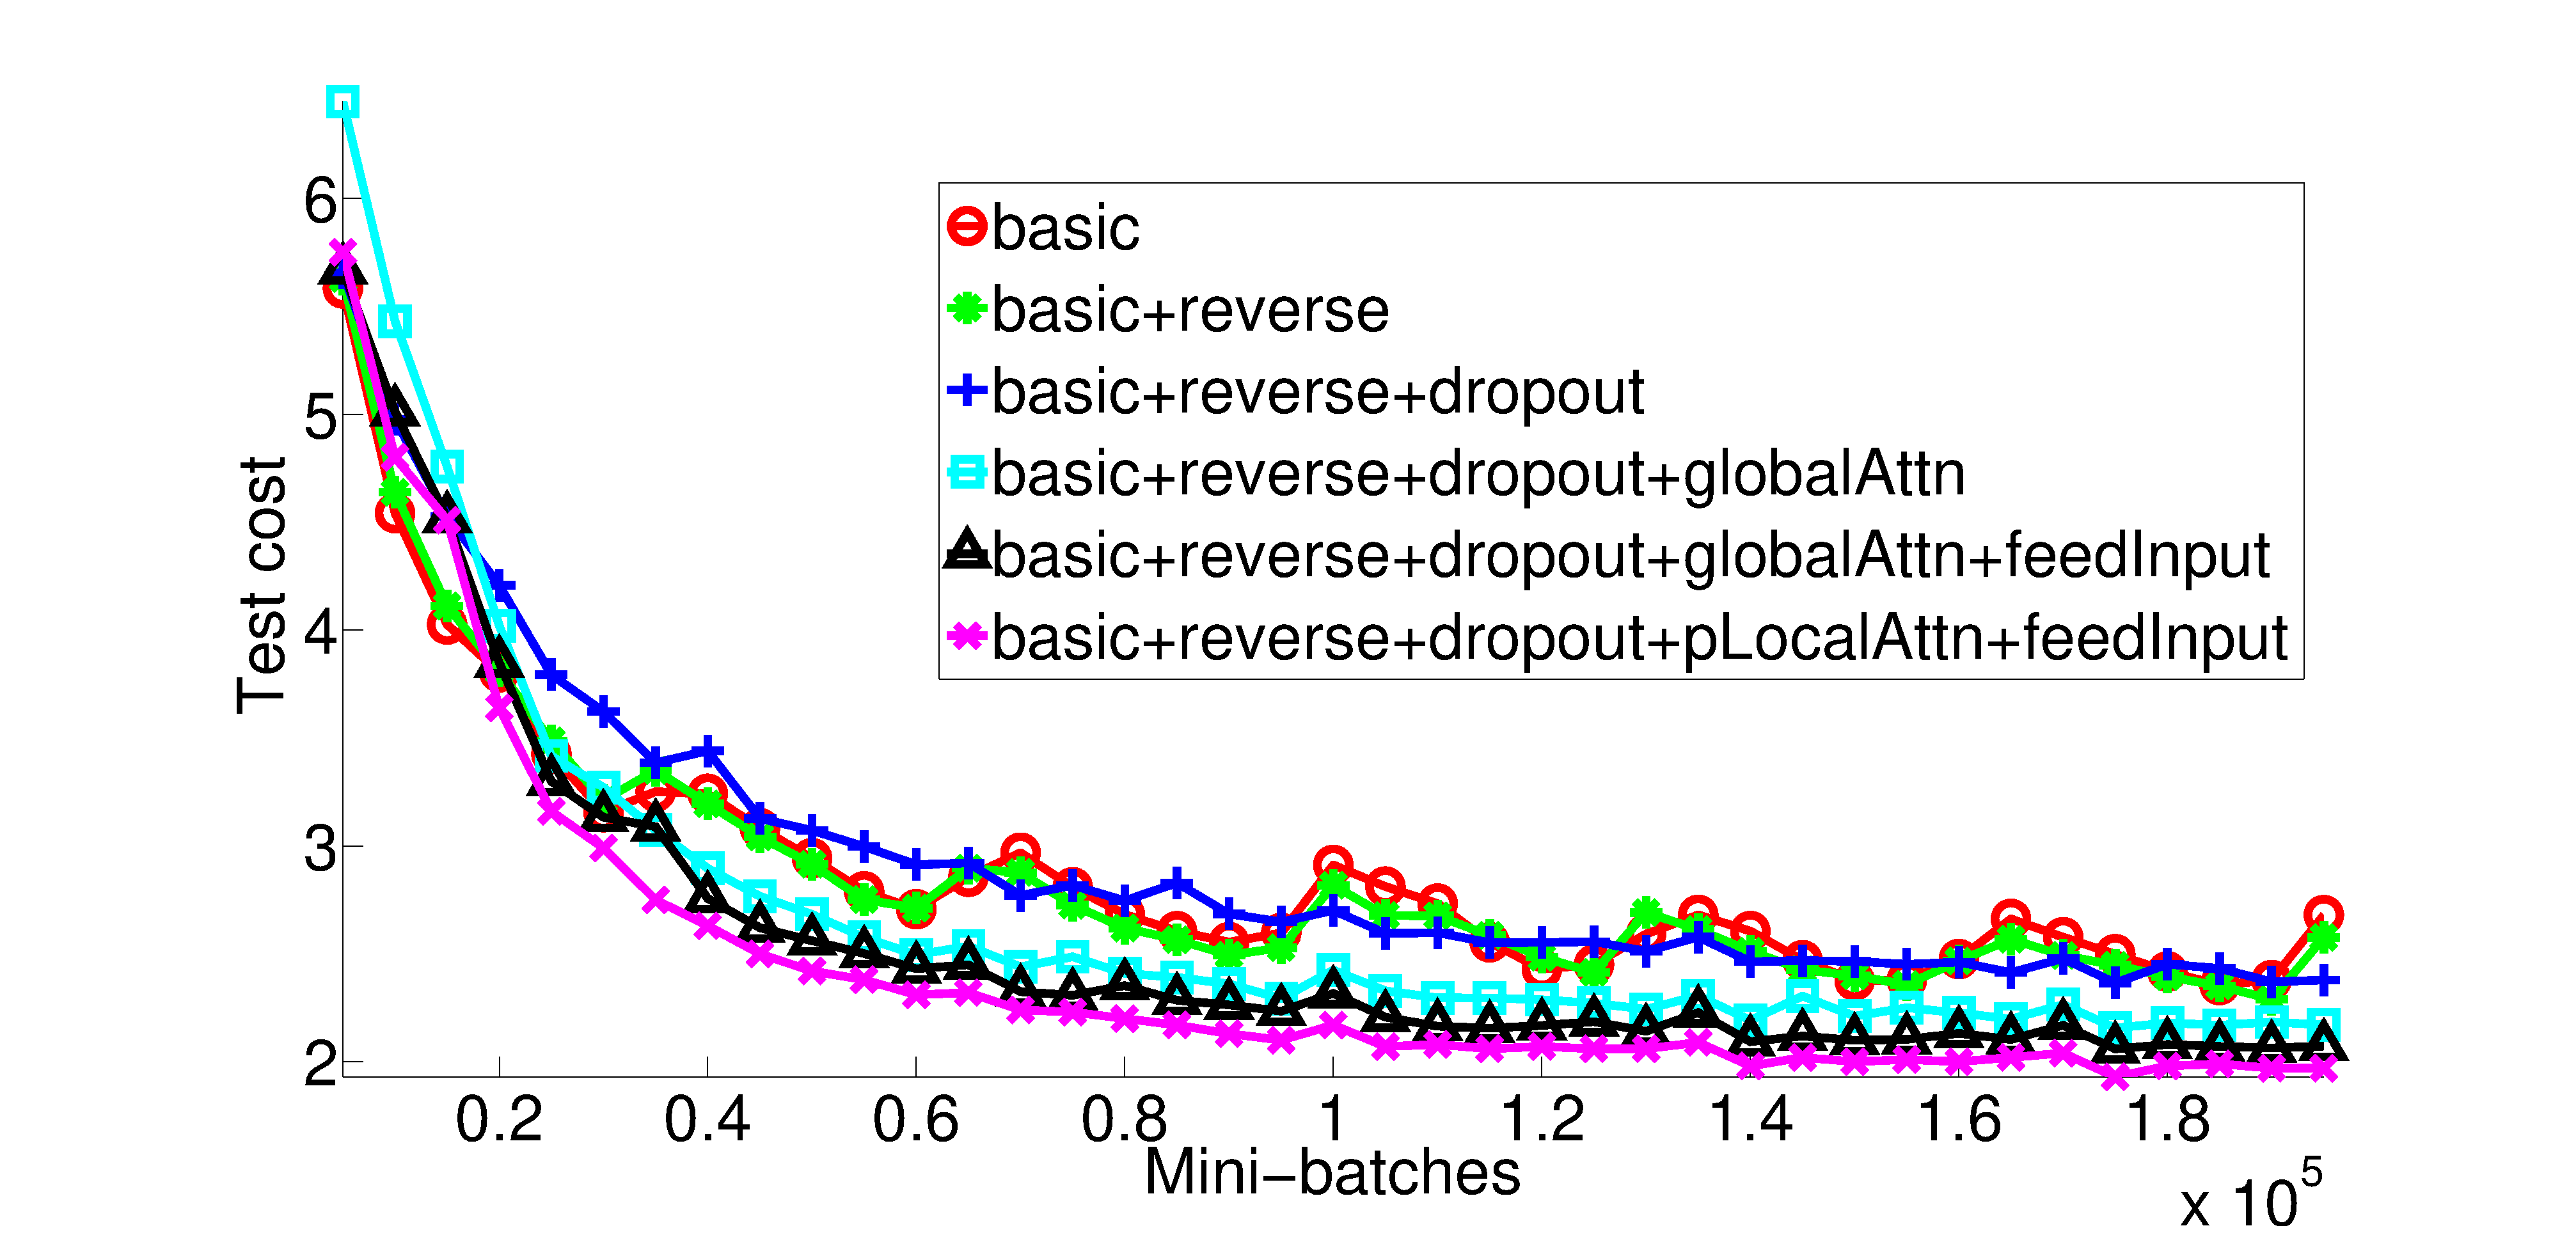
\includegraphics[width=0.7\textwidth, clip=true, trim=140 0 70 0]{img/4-learning} % , angle=-90
\caption[Learning curves]{{\bf Learning curves} -- test cost ($\ln$ perplexity) on newstest2014 for English-German NMTs as training progresses.
} 
\label{f:learn}
\end{figure}

\subsection{Effects of Translating Long Sentences}
I follow \cite{bog15} to group sentences of similar lengths together and
compute a BLEU score per group. Figure~\ref{f:length} shows that
my attentional models are more effective than the non-attentional one in
handling long sentences: the quality does not degrade as sentences
become longer. My best model (the blue + curve) outperforms all other systems in all length buckets.

\begin{figure}[tbh!]
\centering
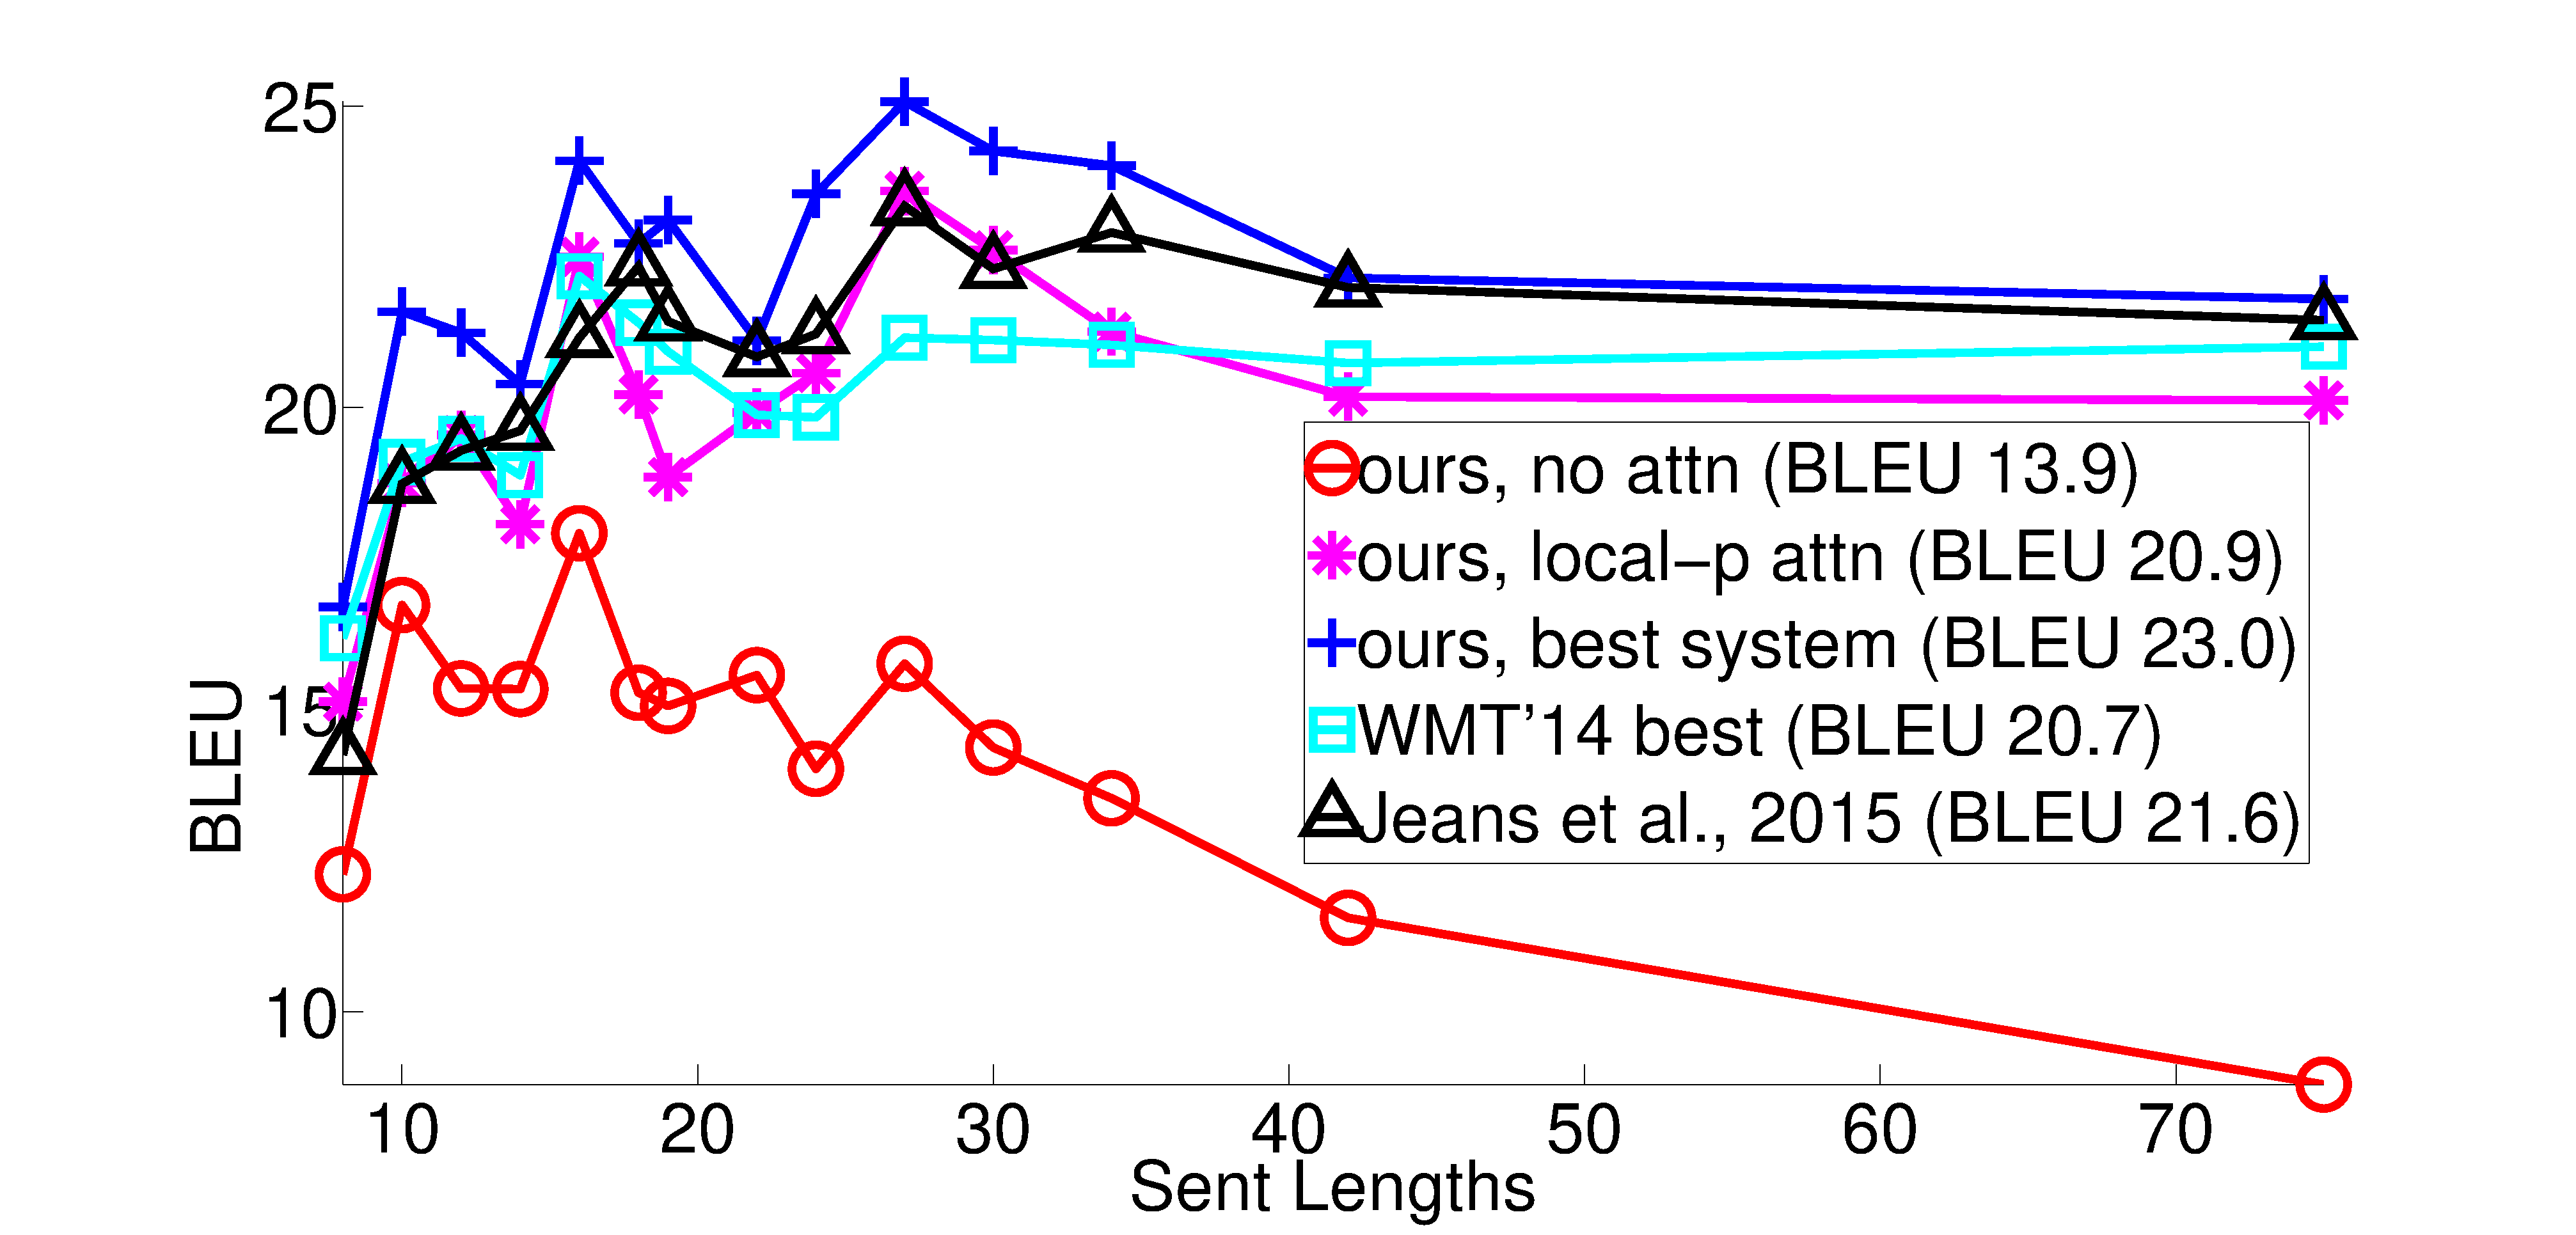
\includegraphics[width=0.7\textwidth, clip=true, trim=120 0 70 0]{img/4-length} % , angle=-90
\caption[Length Analysis]{{\bf Length Analysis} -- translation qualities of different
systems as sentences become longer.
} 
\label{f:length}
\end{figure}

\subsection{Choices of Attentional Architectures}
I examine different attention models ({\it global, local-m, local-p}) and different
alignment functions ({\it location, dot, general, concat}) as described in
Section~\ref{sec:attn}. Due to limited
resources, I cannot run all the possible combinations.
However, results in Table~\ref{t:attnChoices} do give us some idea about
different choices. 
The {\it location-based} function does not learn good
alignments: the {\it global (location)} model can only obtain a small
gain when performing unknown word replacement compared to using other alignment
functions.\footnote{There is a subtle difference in how I retrieve alignments
for the different alignment functions. At time step $t$ in which I receive
$\tgt{t-1}$ as input and then compute $\hi, \al, \co$, and $\hs$ before
predicting $\tgt{t}$, the alignment vector $\al$ is used as alignment
weights for (a) the predicted word $\tgt{t}$ in the {\it location-based}
alignment functions and (b) the input word $\tgt{t-1}$ in the {\it content-based}
functions.}
For {\it content-based} functions, my implementation {\it concat} does not yield good performances
and more analysis should be done to understand the
reason.\footnote{With {\it concat}, the perplexities achieved by different models are 6.7 (global), 7.1
(local-m), and 7.1 (local-p). Such high perplexities could be due to the fact
that I simplify the matrix \MB{W_a} to set the part that corresponds to $\his$
to identity.} It is interesting to observe that {\it dot} works
well for the global attention and {\it general} is better for the local
attention.
Among the different models, the local attention model with predictive alignments ({\it
local-p}) is best, both in terms of perplexities and BLEU.

\begin{table}
\centering
%\resizebox{8cm}{!}{
\begin{tabular}{l|r|c|c}
\multirow{ 2}{*}{\bf{System}} & \multirow{ 2}{*}{\bf{Ppl}} &
\multicolumn{2}{c}{{\bf BLEU}}\\
\cline{3-4}
& & Before & After unk \\
  \hline
global (location) & 6.4 & 18.1 & 19.3 (+1.2) \\
%global (concat) & 6.7 & xx & xx (+xx) \\
global (dot) & 6.1 & 18.6 & 20.5 (+1.9) \\
global (general) & 6.1 & 17.3 & 19.1 (+1.8) \\
  \hline
local-m (dot) & $>$7.0 & x & x \\
local-m (general) & 6.2 & 18.6 & 20.4 (+1.8) \\
  \hline
local-p (dot) & 6.6 & 18.0 & 19.6 (+1.9) \\
local-p (general) & {\bf 5.9} & {\bf 19} & {\bf 20.9 (+1.9)} \\
\end{tabular}
%}
\caption[Attentional Architectures]{{\bf Attentional Architectures} -- performances of different
attentional
models. I trained two local-m (dot) models; both have
ppl $>7.0$.}
\label{t:attnChoices}
\end{table}

\subsection{Alignment Quality}
A by-product of attentional models are word alignments. While \cite{bog15}
visualized alignments for some sample sentences and 
observed gains in translation quality as an indication of a working attention
model, no work has assessed the alignments learned as a whole. In contrast, I
set out to evaluate the alignment quality using the alignment error rate (AER)
metric.

\begin{table}
  \begin{center}
    \begin{tabular}{c c}
      {\bf Method} & {\bf AER} \\
      \hline
      global (location) & $0.39$ \\
      local-m (general)  & $0.34$ \\
      local-p (general) & $0.36$ \\
      \hdashline
      ensemble & $0.34$ \\
      \hline
      Berkeley Aligner & $0.32$ \\
    \end{tabular}
  \end{center}
  \caption[AER scores]{{\bf AER scores} -- results of various models on the RWTH
  English-German alignment data.}
  \label{t:alignment}
\end{table}

Given the gold alignment data provided by RWTH for 508 English-German
Europarl sentences, I ``force'' decode my attentional models to
produce translations that match the references. I extract only one-to-one
alignments by selecting the source word with the highest alignment
weight per target word. Nevertheless, as shown in Table~\ref{t:alignment}, I was able to achieve AER scores
comparable to the one-to-many alignments obtained by the Berkeley aligner
\cite{liang06alignment}.\footnote{I concatenate the 508 sentence pairs with 1M
sentence pairs from WMT and run the Berkeley aligner.}

I also found that the alignments produced by local attention models achieve
lower AERs than those of the global one. The AER obtained by the ensemble, while
good, is not better than the local-m AER, suggesting the well-known
observation that AER and translation scores are not well correlated \cite{fraser07}.

\subsection{Alignment Visualization}
I visualize the alignment weights produced by my different attention
models in Figure~\ref{i:alignment}. The visualization of the local
attention model is much sharper than that of the global one. This contrast matches
my expectation that local attention is designed to only focus on a subset of
words each time. Also, since I
translate from English to German and reverse the source English sentence, the white strides
at the words {\it ``reality''} and {\it ``.''} in the global attention model reveals an
interesting access pattern: it tends to refer back to the beginning of the
source sequence. 

Compared to the alignment visualizations in \cite{bog15}, my 
alignment patterns are not as sharp as theirs. Such difference could possibly be due to
the fact that translating from English to German is
harder than translating into French as done in \cite{bog15},
which is an interesting point to examine in future work.

\begin{figure*}
  \begin{center}
    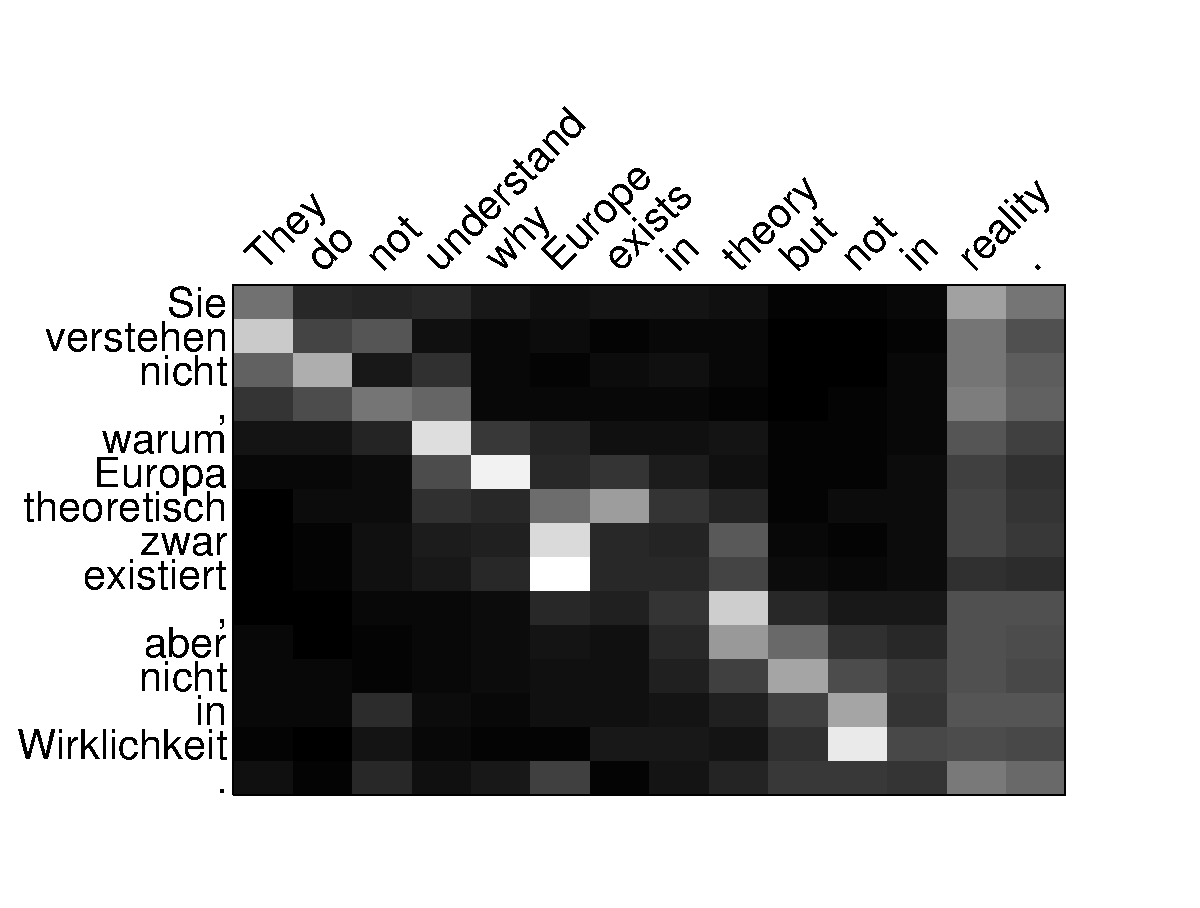
\includegraphics[width=0.48\textwidth]{img/4-align4.eps}
    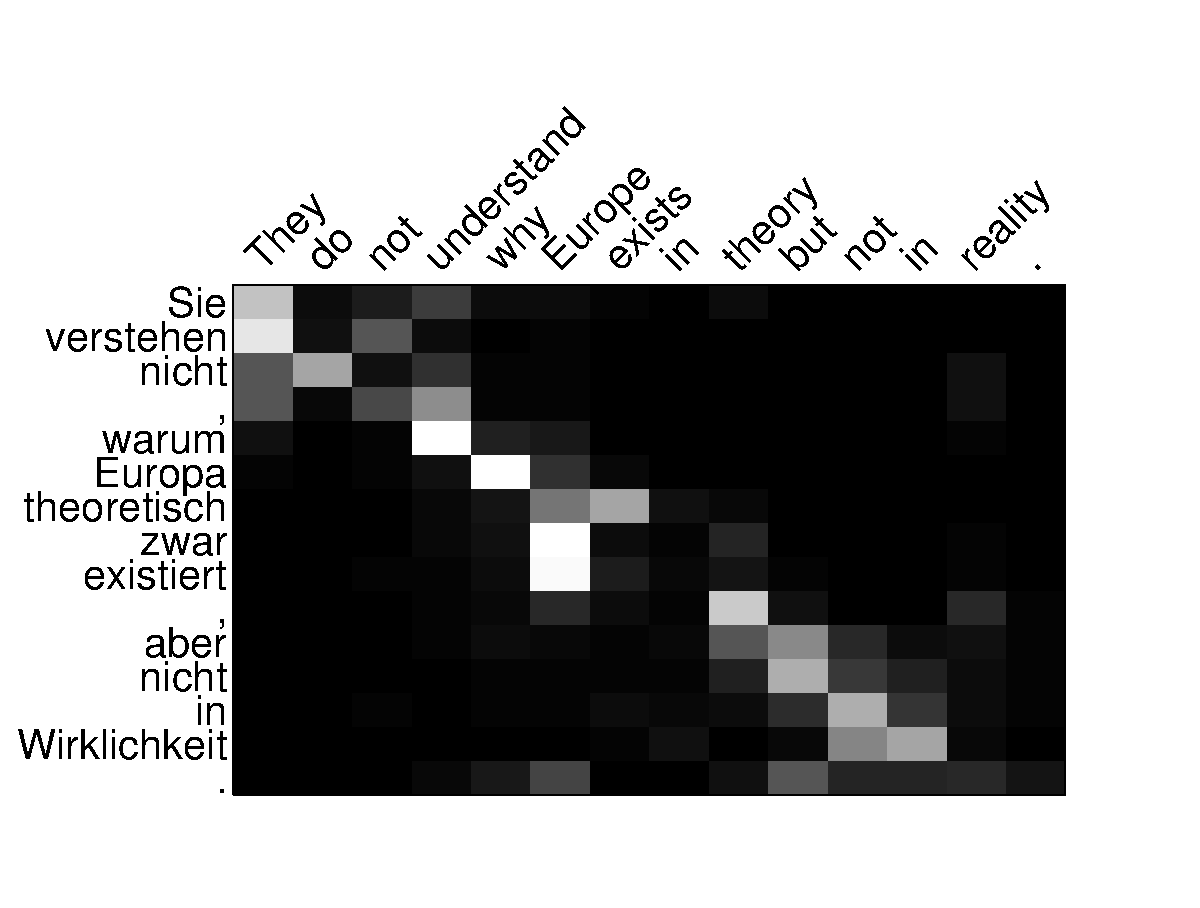
\includegraphics[width=0.48\textwidth]{img/4-align2.eps}
    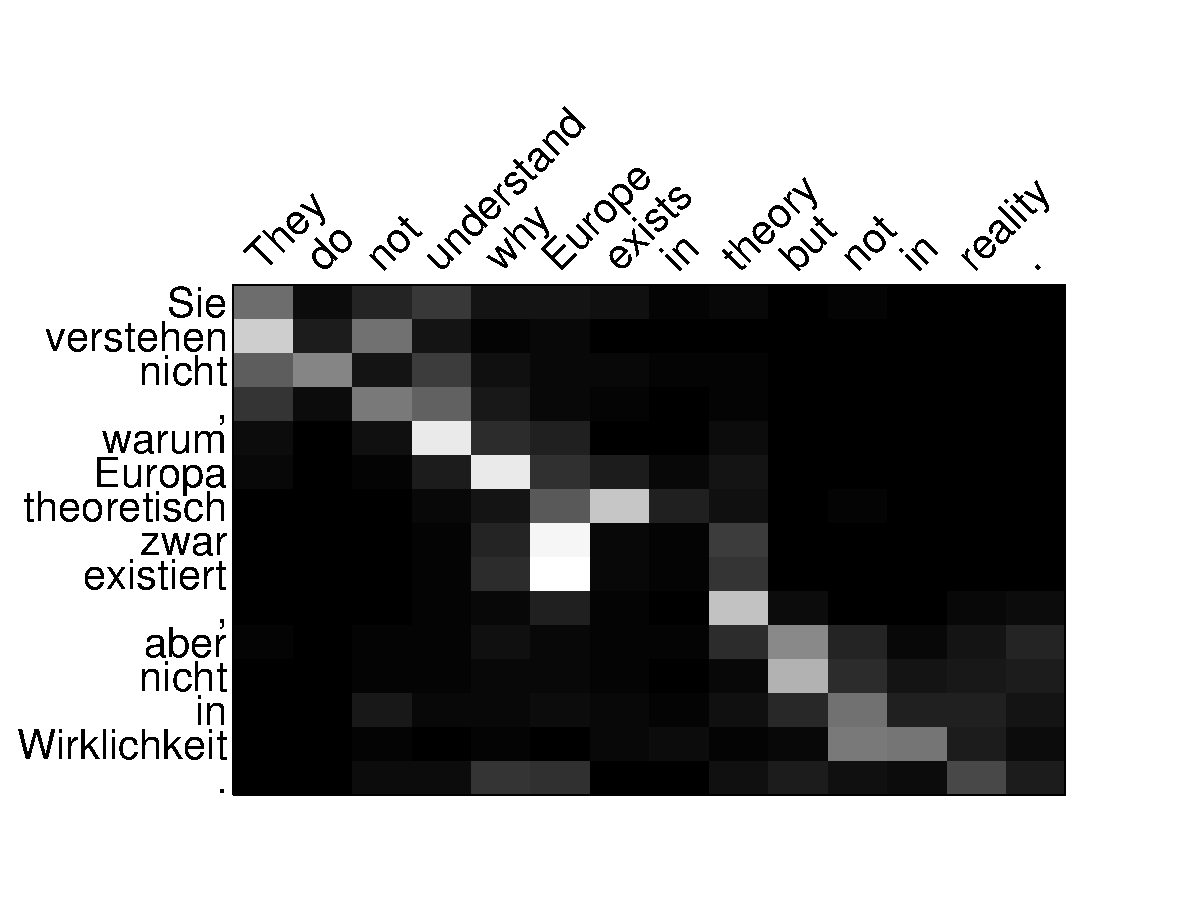
\includegraphics[width=0.48\textwidth]{img/4-align1.eps}
    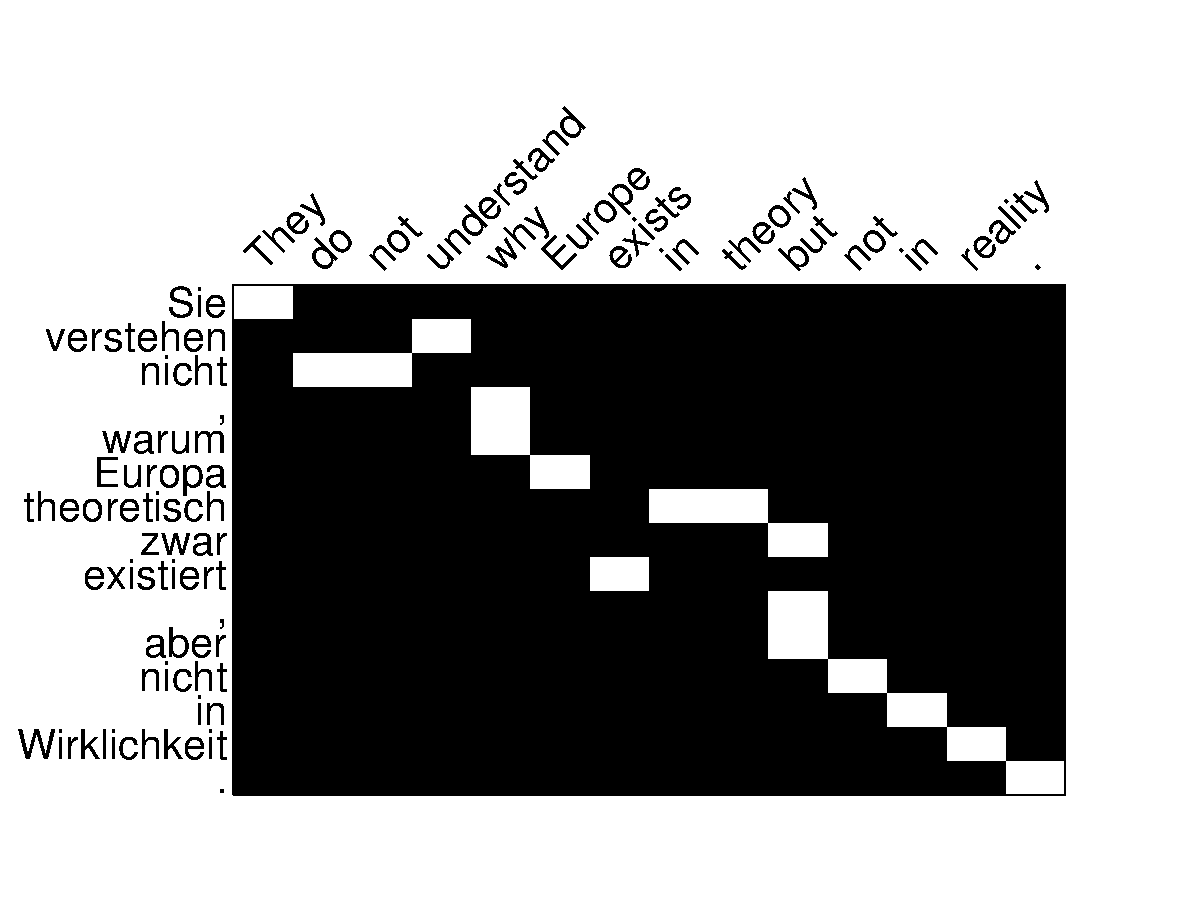
\includegraphics[width=0.48\textwidth]{img/4-alignGold.eps}
  \end{center}
  \caption[Alignment visualizations]{{\bf Alignment visualizations} -- shown are images of the attention
  weights learned by various models: (top left) global, (top right)
  local-m, and (bottom left) local-p. The {\it gold} alignments are
  displayed at the bottom right corner.
  }
  \label{i:alignment}
\end{figure*}

\subsection{Sample Translations}
\label{sec:sample}
I show in Table~\ref{t:sample} sample translations in both directions. It it
appealing to observe the effect of attentional models in correctly translating
names such as ``Miranda Kerr'' and ``Roger Dow''. Non-attentional models, while producing sensible names from a language
model perspective, lack the direct connections from the source side to make
correct translations. % as with the case of attention-based NMT systems. 
I also observed an interesting case in the second
example, which requires translating the {\it doubly-negated} phrase, ``not incompatible''.
The attentional model correctly produces ``nicht $\dots$ unvereinbar'';
whereas the non-attentional model generates ``nicht vereinbar'', meaning
``not compatible''.\footnote{The reference uses a more fancy translation of
``incompatible'', which is ``im Widerspruch zu etwas stehen''. Both models, however, failed to translate ``passenger
experience''.} The attentional
model also demonstrates its superiority in translating long sentences as in
the last example.
\begin{table*}[tbh!]
\centering
\resizebox{15cm}{!}{
\begin{tabular}{c|p{15cm}}
\multicolumn{2}{l}{{\bf English-German translations}}\\
  \hline
src & Orlando Bloom and Miranda Kerr still love each other \\
  \hline
ref & Orlando Bloom und \correct{Miranda Kerr} lieben sich noch immer \\
  \hline
{\it best} & Orlando Bloom und \correct{Miranda Kerr} lieben einander noch immer . \\
  \hline
base & Orlando Bloom und \wrong{Lucas Miranda} lieben einander noch immer .\\
  \hline
  \hline
src & $''$ We $'$ re pleased the FAA recognizes that an enjoyable passenger experience is not incompatible with safety and security , $''$ said Roger Dow , CEO of the U.S. Travel Association . \\
  \hline
ref & `` Wir freuen uns , dass die FAA erkennt , dass ein angenehmes
Passagiererlebnis nicht im Widerspruch zur Sicherheit steht '' , sagte
\correct{Roger Dow} , CEO der U.S. Travel Association . \\
  \hline
{\it best} & $''$ Wir freuen uns , dass die FAA anerkennt , dass ein angenehmes ist
nicht mit Sicherheit und Sicherheit \correct{unvereinbar} ist $''$ , sagte \correct{Roger
Dow} , CEO der US - die . \\
  \hline
base & $''$ Wir freuen uns \"{u}ber die $<$unk$>$ , dass ein $<$unk$>$ $<$unk$>$
mit Sicherheit nicht \wrong{vereinbar} ist mit Sicherheit und Sicherheit $''$ ,
sagte \correct{Roger} \wrong{Cameron} , CEO der US - $<$unk$>$ . \\
  \hline
  \hline
\multicolumn{2}{l}{{\bf German-English translations}}\\
  \hline
src & In einem Interview sagte Bloom jedoch , dass er und Kerr sich noch immer lieben . \\
  \hline
ref & However , in an interview , Bloom has said that he and \correct{Kerr} still love each other . \\
  \hline
{\it best} & In an interview , however , Bloom said that he and \correct{Kerr} still love . \\
  \hline
base & However , in an interview , Bloom said that he and \wrong{Tina} were still $<$unk$>$ . \\
  \hline
  \hline
src & Wegen der von Berlin und der Europ\"{a}ischen Zentralbank verh\"{a}ngten strengen Sparpolitik in Verbindung mit der Zwangsjacke , in die die jeweilige nationale Wirtschaft durch das Festhalten an der gemeinsamen W\"{a}hrung gen\"{o}tigt wird , sind viele Menschen der Ansicht , das Projekt Europa sei zu weit gegangen \\ 
  \hline
ref & The \correct{austerity imposed by Berlin and the European Central Bank , coupled with the straitjacket} imposed on national economies through adherence to the common currency , has led many people to think Project Europe has gone too far .\\
  \hline
{\it best} & Because of the strict \correct{austerity measures imposed by Berlin
and the European Central Bank in connection with the straitjacket} in which the
respective national economy is forced to adhere to the common currency , many
people believe that the European project has gone too far . \\
  \hline
base & Because of the pressure \wrong{imposed by the European Central Bank and the Federal Central Bank with the strict austerity} imposed on the national economy in the face of the single currency , many people believe that the European project has gone too far .\\
\end{tabular}
}
\caption[Sample translations]{{\bf Sample translations} -- %examples in both translation directions.
for each example, I show the source ({\it src}), the human translation ({\it
ref}), the translation from my best model ({\it best}), and the
translation of a non-attentional model ({\it base}).  I italicize some
\correct{correct} translation segments and highlight a few \wrong{wrong} ones in
bold.} % See Appendix~\ref{sec:sample} for detailed descriptions.}
\label{t:sample}
\end{table*}

\section{Conclusion}
\label{sec:conclude}
In this chapter, I propose two simple and effective attentional mechanisms for
neural machine translation: the {\it global} approach which always looks at all
source positions and the {\it local} one that only attends to a subset of source
positions at a time. I test the effectiveness of my models in the WMT
translation tasks between English and German in both directions. 
My local attention yields large gains of up to
$\attngain{}$ BLEU over non-attentional models that already incorporate known
techniques such as dropout. For the English to German translation direction, my
ensemble model has established new state-of-the-art
results for both WMT'14 and WMT'15.

I have compared various alignment functions and shed light on which functions
are best for which attentional models.
My analysis shows that attention-based NMT models are superior to
non-attentional ones in many cases, for example in translating names and
handling long
sentences.


\chapter{Hybrid Models}
\label{c:hybrid}
\begin{sloppypar}
In the previous chapters, I showed that despite being relatively new, NMT has already
achieved state-of-the-art translation results for several language pairs 
such as English-French \cite{luong15}, English-German
\cite{jean15,luong15attn,luong15iwslt}, and English-Czech \cite{jean15wmt}. 
While NMT offers many advantages over traditional phrase-based approaches, such as
small memory footprint and simple decoder implementation, nearly all previous
work in NMT has used quite restricted vocabularies, crudely treating all other
words the same with an \unk{} symbol. Sometimes, a post-processing step that
patches in unknown words is introduced to alleviate this problem. %For example,
In Chapter~\ref{c:copy}, I propose to annotate occurrences of target \unk{} with positional information to
track their alignments, after which simple word dictionary
lookup or identity copy can be performed to replace \unk{} in the translation.
\newcite{jean15} approach the problem similarly but obtain the alignments for unknown
words from the attention mechanism. I refer to these as the {\it
unk replacement} technique.
\end{sloppypar}

\begin{figure}%[tbh]
\centering
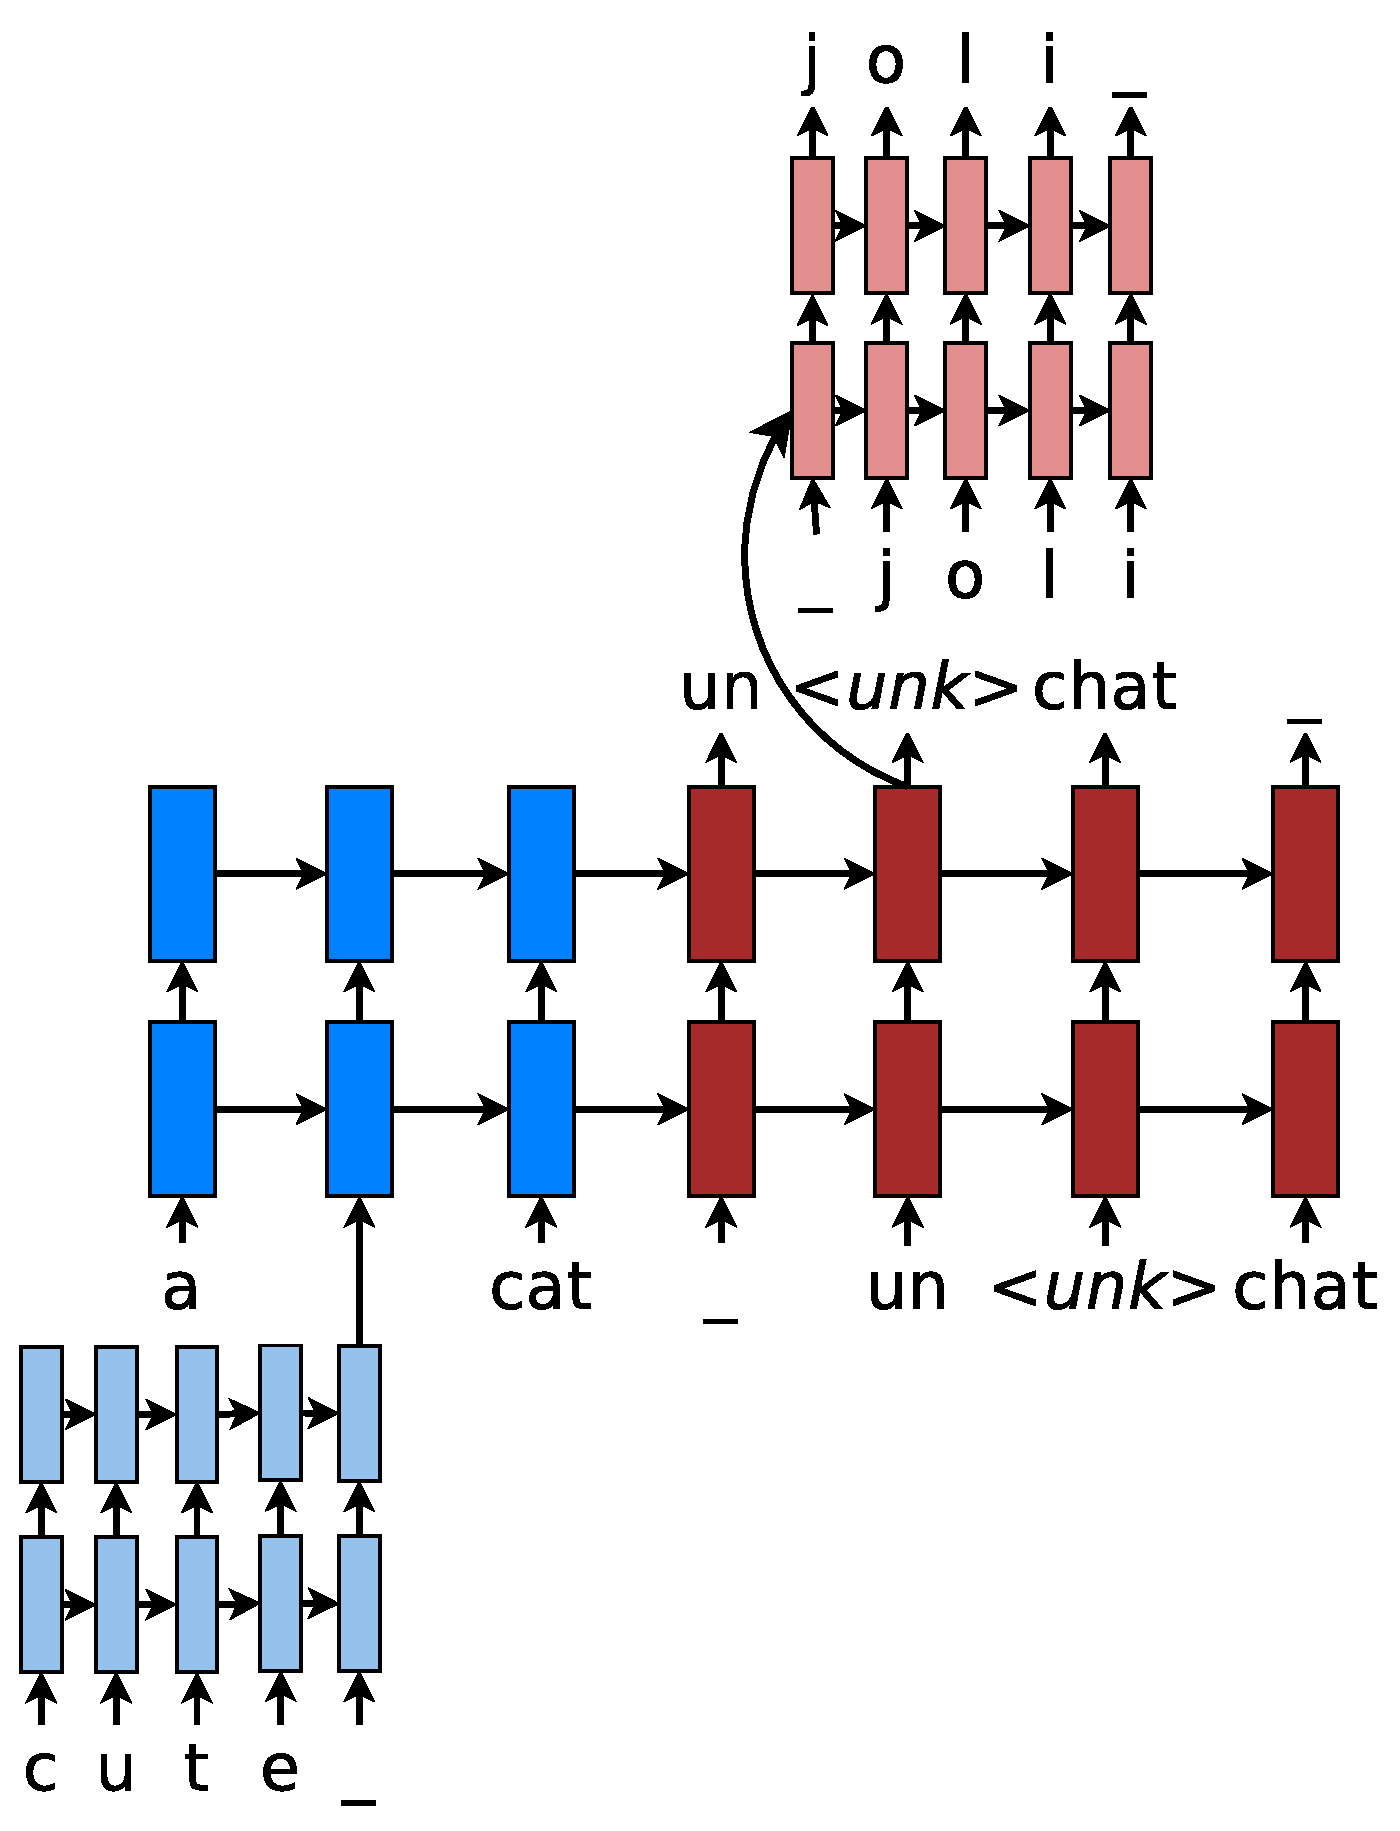
\includegraphics[width=0.6\textwidth, clip=true, trim= 0 0 0 0]{img/5-nmt_hybrid}
\caption[Hybrid NMT]{{\bf Hybrid NMT} -- example of a word-character model for translating
\word{a cute cat} into \word{un
joli chat}. Hybrid NMT translates at the word level. For rare tokens,
the character-level components build source representations
and recover target \unk{}. \word{\_} marks sequence
boundaries.}
\label{f:hybrid}
\end{figure}


Though simple, these approaches ignore several important
properties of languages. First, {\it monolingually}, words are morphologically
related; however, they are currently treated as independent entities. This is
problematic as pointed out by
\newcite{luong13}: neural networks can learn good
representations for frequent words such as \word{distinct}, but fail for
rare-but-related words like \word{distinctiveness}. Second, {\it crosslingually},
languages have different alphabets, so one cannot na\"{i}vely memorize all
possible surface word translations such as name transliteration between 
\word{Christopher} (English) and \word{Kry\u{s}tof} (Czech). See more on this problem
in \cite{sennrich16sub}.

To overcome these shortcomings, I propose a novel {\it hybrid} architecture for NMT
that translates mostly at the word level and consults the character
components for rare words when necessary. As illustrated in
Figure~\ref{f:hybrid}, my hybrid model consists of a word-based NMT that
performs most of the translation job, except for the two (hypothetically) rare words,
\word{cute} and \word{joli}, that are handled separately. On the {\it source}
side, representations for rare words, \word{cute}, are
computed on-the-fly using a deep recurrent neural network that operates at the
character level. On the {\it target} side, I have a separate model that
recovers the surface forms, \word{joli}, of \unk{} tokens character-by-character.
These components are learned jointly end-to-end, removing the need for a separate
unk replacement step as in current NMT practice.

My hybrid NMT offers a twofold advantage: it is much faster and easier to
train than character-based models; at the same time, it never produces unknown
words as in the case of word-based ones.
I demonstrate at scale that on the WMT'15 English to
Czech translation task, such a hybrid approach provides
an additional boost of +$\gain{}$ BLEU points over models 
that already handle unknown words.
I achieve a new state-of-the-art result with
$\ensbleu{}$ BLEU score.
My analysis demonstrates that my character models can successfully learn to not
only generate well-formed words for Czech, a
highly-inflected language with a very complex vocabulary, but also build correct
representations for English source words.

\section{Related Work}
There has been a recent line of work on end-to-end character-based neural models
which achieve good results for part-of-speech tagging \cite{santos14,ling15function},
dependency parsing \cite{ballesteros15}, text classification
\cite{zhang15}, speech recognition \cite{chan16,bahdanau16}, and language
modeling \cite{kim16,rafal16}. However, at the time of this work, success has not been shown for
cross-lingual tasks such as machine translation.
%\footnote{Recently,
%\newcite{ling15char} attempt character-level NMT; however,
%the experimental evidence is weak. The authors demonstrate only small
%improvements over word-level baselines and acknowledge that there are no differences of
%significance. Furthermore, only small datasets were used without
%comparable results from past NMT work.}
\newcite{sennrich16sub} propose to segment words into smaller units and
translate just like at the word level, which does not learn to understand
relationships among words.

My work takes inspiration from \cite{luong13} and 
\cite{li15}. Similar to the former, I build representations for rare words
on-the-fly from subword units. However, instead of using recursive neural
networks with morphemes as units as in \cite{luong13}, which requires existence of a
morphological analyzer, I utilize recurrent neural networks
with characters as the basic units. In comparison with \cite{li15}, my hybrid architecture
is also a hierarchical sequence-to-sequence model, but operates at a different
granularity level, word-character. In contrast, \newcite{li15} build
hierarchical models at the sentence-word level for paragraphs and documents.

\section{Hybrid Neural Machine Translation}
\label{sec:hybrid}
My hybrid architecture, illustrated in Figure~\ref{f:hybrid}, leverages the power of both words
and characters to achieve the goal of open vocabulary NMT. The core of the
design is a {\it word}-level NMT with the advantage of being fast and easy to
train.
The {\it character} components empower the 
word-level system with the abilities to compute any source word representation on the fly from 
characters and to recover character-by-character unknown target words
originally produced as \unk{}.

\subsection{Word-based Translation as a Backbone}
\label{subsec:hybrid_word}
The core of my hybrid NMT is a deep LSTM encoder-decoder that translates at
the {\it word} level as described in Chapter~\ref{c:background}. I maintain a
vocabulary of $|V|$ frequent words for each language. Other words not inside these
lists are represented by a universal symbol \unk{}, one per language.
I translate just like a word-based NMT system with respect to these source and
target vocabularies, except for cases that involve \unk{} in the source input or 
the target output. These correspond to the character-level components 
illustrated in Figure~\ref{f:hybrid}.
A nice property of my hybrid approach is that by varying the vocabulary size,
 one can control how much to blend the
word- and character-based models; hence, taking the best of both
worlds. 


\subsection{Source Character-based Representation}
\label{subsec:src}
In regular word-based
NMT, for all rare words outside the source vocabulary, one feeds the
universal embedding representing \unk{} as input to the encoder. This is
problematic because it discards valuable information about the source word. To
fix that, I learn a deep LSTM model over characters
of source words. 
For example, in Figure~\ref{f:hybrid}, I run
my deep character-based LSTM over `c', `u', `t', `e', and `\_' (the boundary
symbol). The final hidden state at the top layer will be used as the on-the-fly
representation for the current rare word.
The layers of the deep character-based LSTM are always initialized with {\it
zero} states. One might propose to connect hidden
states of the word-based LSTM to the character-based model; however, I chose this design
for various reasons. First, it simplifies the architecture. Second, it allows
for efficiency through {\it precomputation}: before each mini-batch, I can compute
representations for rare source words all at once. All instances of the same
word share the same embedding, so the computation is per {\it type}.\footnote{While \newcite{ling15char} found that it is slow and difficult to train
source character-level models and had to resort to pretraining, I demonstrate
later that I can train my deep character-level LSTM
perfectly fine in an end-to-end fashion.} 

\subsection{Target Character-level Generation}
\label{subsec:tgt}
General word-based NMT allows generation of \unk{} in the target output.
Afterwards, there is usually a post-processing step that handles
these unknown tokens by utilizing the
alignment information derived from the attention mechanism and then performing
simple word dictionary lookup or identity copy \cite{luong15attn,jean15}. 
While this approach works, it suffers from various problems such as alphabet
mismatches between the source and target vocabularies and multi-word
alignments.
My goal is to address all
these issues and create a
coherent framework that handles an unlimited output vocabulary.

My solution is to have a separate deep LSTM that ``translates'' at the
character level given the current word-level state. I train my system such
that whenever the word-level NMT
produces an \unk{}, I can consult this character-level decoder to recover the correct surface form of the
unknown target word. This is illustrated in Figure~\ref{f:hybrid}.
The training objective for the hybrid models consists of two components:
\begin{equation}
J = J_{w} + \alpha J_{c}
\label{e:char_obj}
\end{equation}
Here, $J_{w}$ refers to the usual loss of the word-level NMT; in
my example, it is the sum of the negative log likelihood of
generating $\{\mbox{``un'', ``\unk{}'', ``chat'', ``\_''}\}$. The remaining component $J_c$
corresponds to the loss incurred by the character-level 
decoder when predicting characters, e.g., $\{\mbox{`j', `o', `l', `i',
`\_'}\}$, of those rare words not in the
target vocabulary. 


\paragraph{Hidden-state Initialization}
\label{subsubsec:h}
\begin{figure}
\centering
%\psgrid
\rput(5.6,8.3){$\tgt{t}$}
\rput(1.8,7.2){$\co$}
\rput(1.0,4.1){$\hb{1}$}
\rput(3.7,4.1){$\hb{n}$}
\rput(6.4,4.1){$\hd{t}$}
\rput(6.4,7.8){$\hs$}
%\rput(4.0,3.8){$\hd{t-1}$}
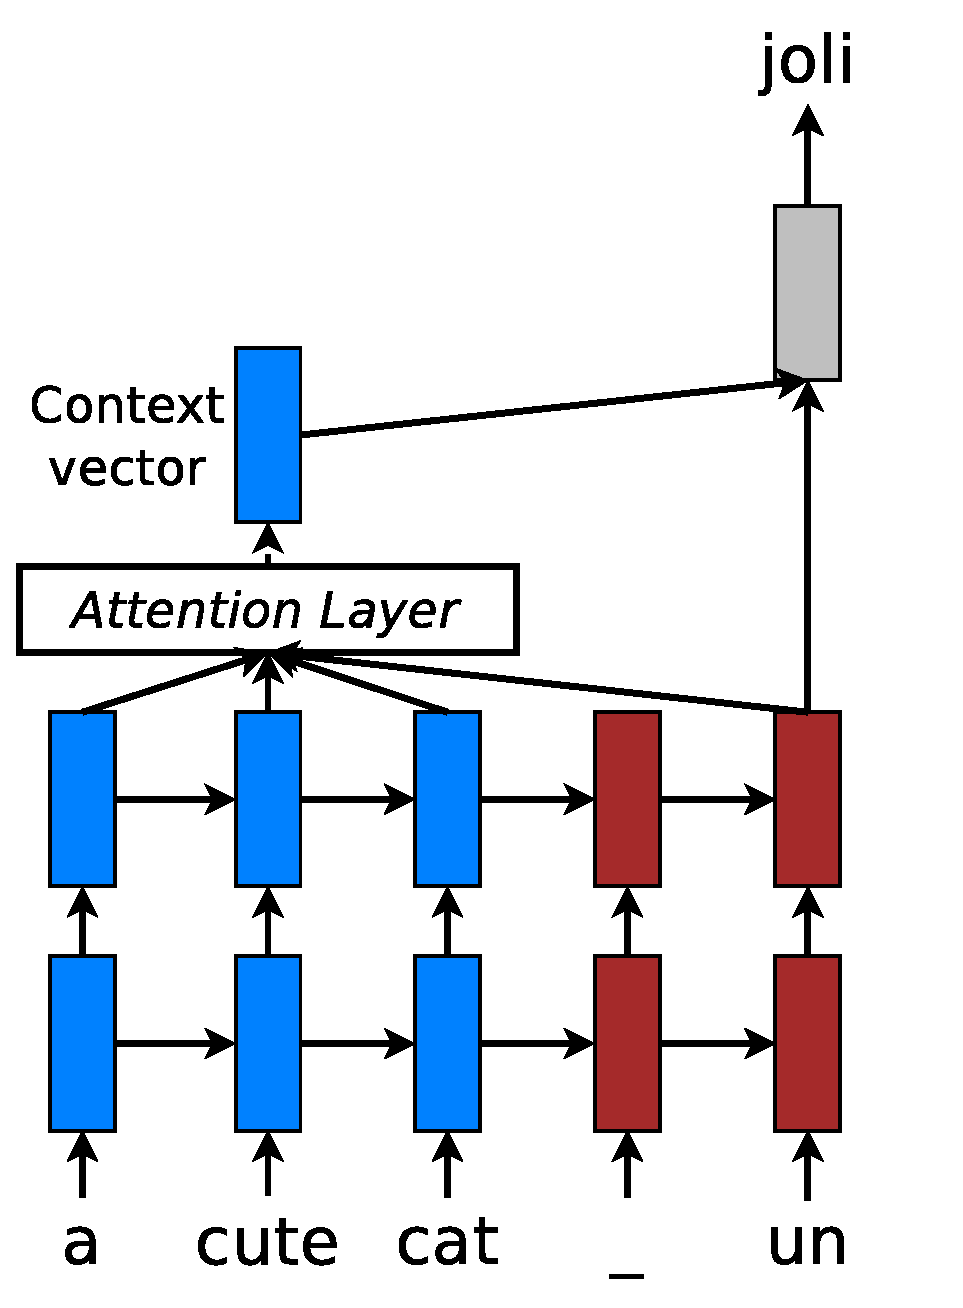
\includegraphics[width=0.45\textwidth, clip=true, trim= 0 0 0 0]{img/5-attn} % , angle=-90
\caption[Attention mechanism]{{\bf Attention mechanism} -- shown are the two steps of the
attention mechanism I described in Chapter~\ref{c:attention} \cite{luong15attn}: first, compute a 
{\it context vector} $\co$ based on the current target hidden state $\hd{t}$ and all the source hidden
states $[\hb{1}, \dots, \hb{n}]$; second, use the context vector as an
additional input to derive
the {\it attentional} vector $\hs$.
} 
\label{f:attn}
\end{figure}

Unlike the source character-based representations, which are
context-independent, the target character-level generation requires the
current word-level context to produce meaningful translation.
This brings up an important
question about what can best represent the current context so as to
initialize the character-level decoder. I answer this question in the context
of the attention mechanism described in Chapter~\ref{c:attention}. 

The final vector $\hs$, just before the
softmax as shown in Figure~\ref{f:attn}, seems to be a good candidate to initialize the character-level decoder.
The reason is that $\hs$ combines
information from both the context vector $\co$ and the top-level recurrent
state $\hi$. I refer to it later in my
experiments as the \textit{same-path} target generation approach.

On the other hand, the same-path approach worries us because all vectors $\hs$
used to seed the character-level decoder might have similar values, leading to
the same character sequence being produced.
The reason is because $\hs$ is directly used in the softmax, \eq{e:softmax}, to predict the same \unk{}.
That might pose some challenges for the model to learn useful representations
that can be used to accomplish two tasks at the same time, that is to predict
\unk{} and to generate character sequences.
To address that concern, I propose another approach called
the \textit{separate-path} target generation.

\begin{figure}%[tbh]
\centering
%\psgrid
\rput(1.8,4.9){$\co$}
\rput(3.2,4.6){$\Wc$}
\rput(5.4,4.6){$\Ww$}
\rput(6.25,1.8){$\hi$}
\rput(3.75,6){$\hc$}
\rput(6.25,6){$\hs$}
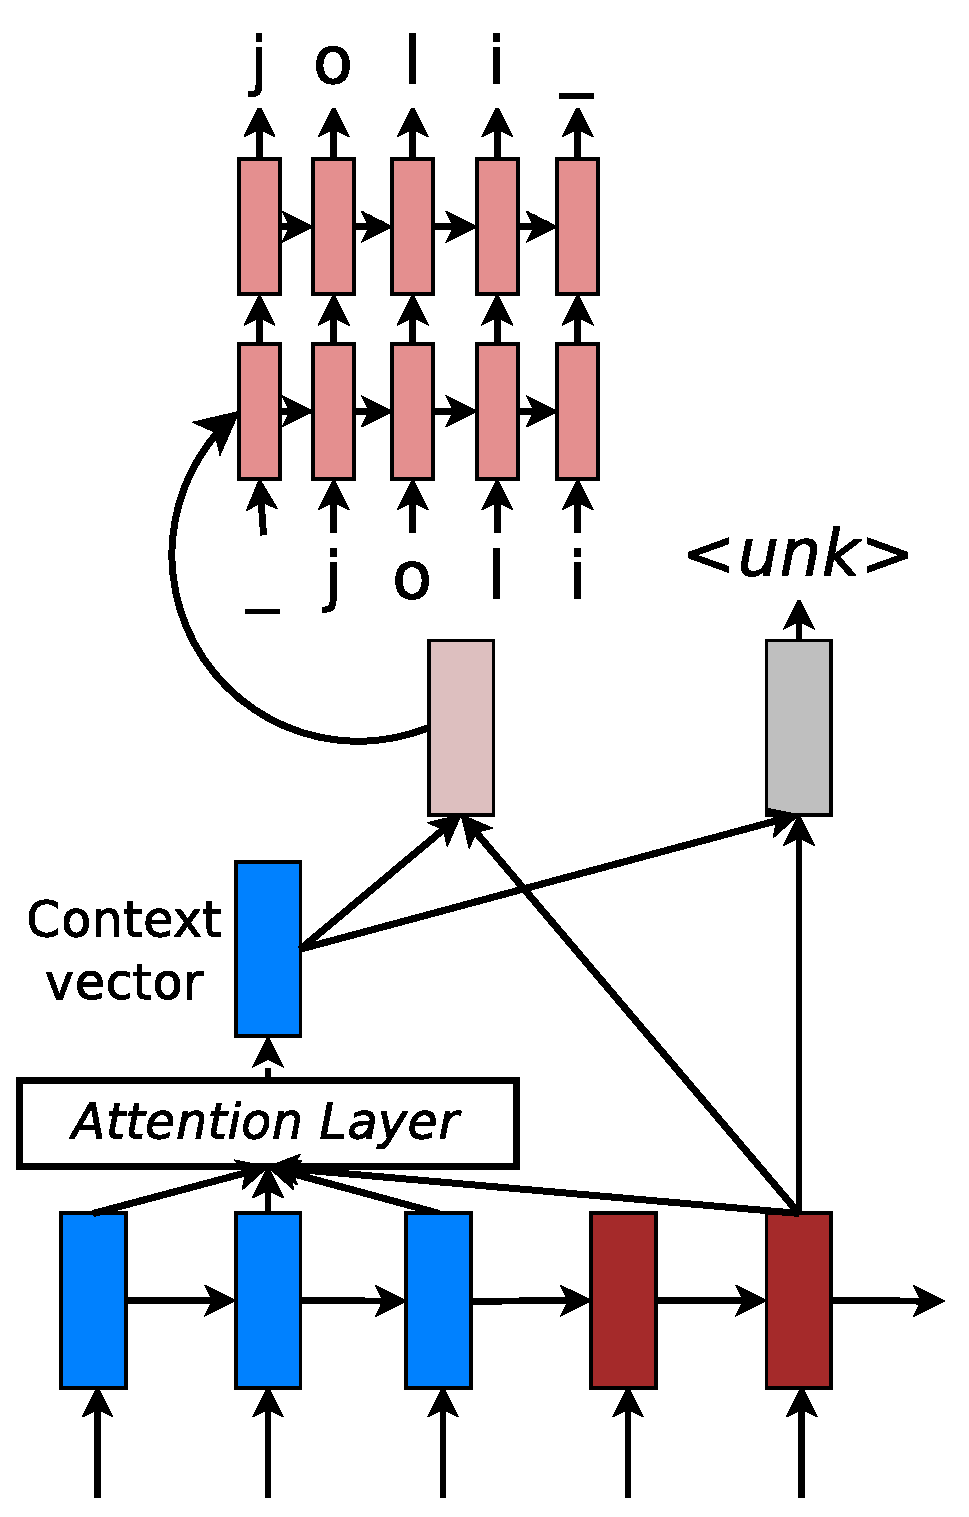
\includegraphics[width=0.45\textwidth, clip=true, trim= 0 0 0 0]{img/5-tgtGen}
\caption[Separate-path target generation]{{\bf Separate-path target generation} -- two separate attentional vectors are creating:
$\hs$ for predicting target words and $\hc$ to seed the target-side character model.}
\label{f:tgtGen}
\end{figure}

My separate-path target generation approach works as follows. I mimic the
process described in \eq{e:hs} of the attention mechanism to create a counterpart vector $\hc$ that will be
used to seed the character-level decoder:
\begin{equation}
\hc = \tanh(\Wc[\co; \hi])
\label{e:hc}
\end{equation} 
Here, $\Wc$ is a new learnable parameter matrix, with which I
hope to release $\W{}$ from the pressure of having to extract information
relevant to both the word- and character-generation processes.
This approach is illustrated in Figure~\ref{f:tgtGen}.
Only the hidden
state of the first layer is initialized as discussed above. The other components
in the character-level decoder such as the
LSTM cells of all layers and the hidden states of higher layers, all start with zero values.

Implementation-wise, the computation in the
character-level decoder is done per word {\it token} instead of per {\it type} as in the source
character component ($\S$\ref{subsec:src}). 
This is because of the context-dependent nature of the decoder.
\footnote{To be memory efficient, the character-level backward pass can be executed right
after the character-level forward pass
and we can split these computations into
mini-batches if the number of \unk{} is large.}

\paragraph{Word-Character Generation Strategy}
\label{subsubsec:strategy}
With the character-level decoder, we can view the final hidden states as representations for
the surface forms of unknown tokens and could have fed these to the next
time step. However, I chose not to do so for the efficiency reason explained
next; instead, \unk{} is fed to the word-level decoder
``as is'' using its corresponding word embedding.

During {\it training}, this design choice decouples all executions over \unk{} instances of the
character-level decoder as soon the word-level NMT
completes. As such, the forward and backward passes of the character-level
decoder over rare words can be invoked in batch mode. At {\it test} time,
my strategy is to first run a beam search decoder at the word level to
find the best translations given by the
word-level NMT. Such translations contains \unk{} tokens, so I utilize the 
character-level decoder with beam search to generate actual words for these \unk{}.

\section{Experiments}
\label{sec:exp}
I evaluate the effectiveness of my models on the publicly available WMT'15
translation task from English into Czech with 
{\it newstest2013} (3000 sentences) as
a development set % to select my hyperparameters. 
and {\it newstest2015} (2656 sentences) as a test set. Two metrics are used: case-sensitive NIST BLEU \cite{Papineni02bleu}
and \chr{} \cite{chrf}.\footnote{For NIST BLEU, I first run
\texttt{detokenizer.pl} % with default setting 
and then use \texttt{mteval-v13a}
to compute the scores as per WMT guideline. For \chr{}, I utilize the implementation here
\url{https://github.com/rsennrich/subword-nmt}.}
The latter measures the amounts of overlapping character $n$-grams and has
been argued to be a better metric for translation tasks out of English.

\subsection{Data}
Among the available language pairs in WMT'15, all involving English, 
I choose {\it Czech} as a target language for several reasons. First and
foremost, Czech is a Slavic language with not only rich
and complex inflection,
but also fusional morphology in which a single morpheme can encode multiple
grammatical, syntactic, or semantic meanings. As a result, Czech possesses an enormously large
vocabulary (about 1.5 to 2 times bigger than that of English according to 
statistics in Table~\ref{t:data}) and is a challenging language to translate
into. Furthermore, this language pair has a large
amount of training data, so %, much bigger than English-Finnish and English-German
I can evaluate at scale. Lastly, though my techniques are language
independent, it is easier for us to work with Czech since Czech uses the Latin alphabet with some
diacritics. % than Russian 

\begin{table} %[tbh!]
\centering
%\resizebox{8cm}{!}{
\begin{tabular}{l|c|c|c|c}
& \multicolumn{2}{c|}{\bf{English}} & \multicolumn{2}{c}{\bf{Czech}}\\
  \cline{2-5}
& word & char & word & char \\
  \hline
  \# Sents & \multicolumn{4}{c}{15.8M} \\
  \hdashline
  \# Tokens & 254M & 1,269M & 224M & 1,347M \\ 
% \hline
% \multicolumn{5}{c}{\biformat{Full}} \\
 \hdashline
  \# Types & 1,172K & 2003 & 1,760K & 2053\\ 
  \hline
  200-char & \multicolumn{2}{c|}{98.1\%} & \multicolumn{2}{c}{98.8\%} \\
\end{tabular}
%}
\caption[WMT'15 English-Czech data]{{\bf WMT'15 English-Czech data} -- shown are various statistics of my training
data such as {\it sentence}, {\it token} (word and character counts), as well as
{\it type} (sizes of the word and character vocabularies).
I show in addition the amount of words in a vocabulary expressed by a list of 200 characters found
in frequent words.}
\label{t:data}
\end{table}

In terms of preprocessing, I apply only the standard tokenization practice.\footnote{I use \texttt{tokenizer.perl} in Moses with
default settings.} I choose for each language a list of 200
characters found in frequent words, which, as shown in Table~\ref{t:data}, can
represent more than 98\% of the vocabulary. 

\begin{table*}%[tbh!]
\centering
\resizebox{15cm}{!}{
\begin{tabular}{c|l|c|c|c|c|c}
 & \multirow{2}{*}{\bf{System}} & \multirow{2}{*}{{\bf
 Vocab}} &
\multicolumn{2}{c|}{{\bf Perplexity}} &\multirow{ 2}{*}{\bf{BLEU}} &\multirow{
2}{*}{\bf{\chr{}}}\\
\cline{4-5}
& & & w & c & & \\
  \hline
(a) & Best WMT'15, big data \cite{bojar15wmt} & % -- {\it large data}
- & - & - & \biformat{18.8} & - \\
  \hline
\multicolumn{7}{c}{{\it Existing} NMT}\\
  \hline
(b) & RNNsearch + unk replace \cite{jean15wmt} & 200K & - & - & 15.7 & - \\
%  \hdashline
(c) & \biformat{Ensemble} 4 models + unk replace \cite{jean15wmt} & 200K & - & - & 18.3 & - \\
  \hline
\multicolumn{7}{c}{My {\it word-based} NMT}\\
  \hline
%(d) & Base & 50K & - & 8.7 & - & 12.6 & 32.8\\
%  \hdashline
(d) & Base + attention + unk replace & 50K & 5.9 & - & 17.5 & 42.4 \\
%  \hdashline
(e) & \biformat{Ensemble} 4 models + unk replace & 50K & - & - & 18.4 & 43.9 \\
  \hline
\multicolumn{7}{c}{My {\it character-based} NMT}\\
  \hline
(f) & Base-512 (600-step backprop) & 200 & - & 2.4 & 3.8 & 25.9\\
(g) & Base-512 + attention (600-step backprop) & 200 & - & 1.6 & 17.5 &
\biformat{46.6} \\
  \hdashline
(h) & Base-1024 + attention (300-step backprop) & 200 & - & 1.9 & 15.7 & 41.1 \\
  \hline
\multicolumn{7}{c}{My {\it hybrid} NMT}\\
  \hline
%(j) & Base + attention + same-path & 1K & 200 & 3.3 & 1.72 & 12.9 (5.0) & 36.3\\
% \hdashline
(i) & Base + attention + same-path & 10K & 4.9 & 1.7 & 14.1 & 37.2 \\
(j) & Base + attention + separate-path & 10K & 4.9 & 1.7 & 15.6 & 39.6 \\
(k) & Base + attention + separate-path + 2-layer char & 10K & 4.7 & 1.6 & \biformat{17.7} & 44.1 \\
% (m) & Base + attention + {\it separate}-path + 2-layer char & 10K & 200 & 4.6 & {\bf 1.59} & \biformat{17.5} (11.3) & 43.4 \\
  \hdashline
(l) & Base + attention + separate-path + 2-layer char & 50K & 5.7 & 1.6 & 19.6 & 46.5 \\
%(n) & Base + attention + {\it separate}-path & 50K & 6.2 & 1.73 & 18.0 (15.5) & 44.4 \\
(m) & \biformat{Ensemble} 4 models & 50K & - & - & {\bf \ensbleu{}} & {\bf 47.5} \\
\end{tabular}
}
\caption[WMT'15 English-Czech results]{{\bf WMT'15 English-Czech results} -- shown are 
the vocabulary sizes, perplexities, BLEU, and \chr{} scores of various systems on
{\it newstest2015}. Perplexities are listed under two
categories, word (w) and character (c). 
% For BLEU scores, I report results before \unk{} tokens are handled in parentheses. 
{\bf Best} and
\biformat{important} results per
metric are highlighted.
% and give {\it progressive} improvements in italic between
% consecutive systems.  
}
\label{t:encs}
\end{table*}


\subsection{Training Details}
I train three types of systems, purely {\it word-based}, purely {\it
character-based}, and {\it hybrid}.
Common to these architectures is a word-based NMT since the
character-based systems are essentially word-based ones with
longer sequences and the core of hybrid models is also a word-based NMT.

In training word-based NMT, I proceed as in Chapter~\ref{c:attention} \cite{luong15attn} to use the global attention mechanism together with
similar hyperparameters: (a) deep LSTM models, 4 layers, 1024
cells, and 1024-dimensional embeddings, (b) uniform initialization of
parameters in $[-0.1, 0.1]$, (c) 6-epoch training with plain SGD and a simple learning
rate schedule -- start with a learning rate of $1.0$; after 4 epochs,
halve the learning rate every 0.5 epoch, (d) mini-batches are of
size 128 and shuffled, (e) the gradient is rescaled whenever its norm exceeds 5, and (f)
dropout is used with probability $0.2$ according to 
\cite{pham2014dropout}.
I now detail differences across the three architectures.

{\bf Word-based NMT} -- I constrain my source and target sequences to
have a maximum length of 50 each; words that go past the boundary are ignored.
The vocabularies are limited to the top $|V|$ most
frequent words in both languages. Words not in these vocabularies
are converted into \unk{}. After translating, I will perform
dictionary\footnote{Obtained from the alignment links produced by the Berkeley
aligner \cite{liang06alignment} over
the training corpus.} lookup or
identity copy for \unk{} using the alignment information from the
attention models. Such a procedure is referred to as the {\it unk replace}
technique as in Chapter~\ref{c:copy} \cite{luong15,jean15}.

{\bf Character-based NMT} -- The source and
target sequences at the character level are often about 5 times longer than their counterparts in the
word-based models as can be inferred from the statistics in
Table~\ref{t:data}. Due to the memory constraint in GPUs, I limit my source and
target sequences to a maximum length of 150 each, i.e., I backpropagate
through at most 300 timesteps from the decoder to the encoder. With
smaller 512-dimensional models, I can afford to have longer sequences with up
to 600-step backpropagation. 

{\bf Hybrid NMT} -- The {\it word}-level component uses the
same settings as the purely word-based NMT. For the {\it character}-level source
and target components, I experiment with both shallow and deep 1024-dimensional models of
1 and 2 LSTM layers. 
I
set the weight $\alpha$ in \eq{e:char_obj} for my character-level loss to
$1.0$.

{\bf Training Time} -- It takes about 3 weeks to train a word-based model with
$|V|=50K$ and about 3 months to train a character-based model. Training and
testing for the hybrid models are about 10-20\% slower than those of the word-based
models with the same vocabulary size.

\subsection{Results}

I compare my models with several strong systems. These include the
winning entry in WMT'15, which was
trained on a much larger amount of data, 52.6M parallel
 and 393.0M monolingual sentences \cite{bojar15wmt}.\footnote{This
entry combines two independent
systems, a phrase-based Moses model and a deep-syntactic transfer-based model.
Additionally, there is  an automatic
post-editing system with hand-crafted rules to correct errors
in morphological agreement and semantic meanings, e.g., loss of negation.}
In contrast, I merely use the
provided parallel corpus of 15.8M sentences.
For NMT, to the best of my knowledge, \cite{jean15wmt} has
the best published performance on English-Czech.

As shown in Table~\ref{t:encs}, for a purely {\it word-based} approach, 
my single NMT model outperforms the best single model in \cite{jean15wmt} by
+$1.8$ points despite
using a smaller vocabulary of only 50K words versus 200K words. 
My ensemble system {\it (e)} slightly outperforms the best previous NMT system with $18.4$ BLEU.

To my surprise, purely {\it character-based} models, though extremely slow to
train and test, perform quite well. The $512$-dimensional attention-based model \modelchar{} is
best, surpassing the single word-based model in
\cite{jean15wmt} despite having much fewer parameters. It even outperforms most NMT
systems  
on \chr{} with $46.6$ points. This indicates that this model translate words that closely but
not exactly match the reference ones as evidenced in
Section~\ref{subsec:samples}. 
I notice two interesting observations. First,
attention is critical for character-based models to work as is obvious from the
poor performance of the non-attentional model; this has also been shown in speech
recognition \cite{chan16}. Second, long time-step backpropagation is more important
as reflected by the fact that the larger $1024$-dimensional model {\it (h)} with shorter
backprogration is inferior to \modelchar{}. 

My {\it hybrid} models achieve the best results. 
At 10K words, I demonstrate that my {\it
separate-path} strategy for the character-level target generation
($\S$\ref{subsubsec:h}) is effective, yielding an improvement of +$1.5$ BLEU
points when comparing systems {\it (j)} vs. {\it (i)}. A {\it deeper} character-level architecture of 2 LSTM
layers provides another significant
boost of +$2.1$ BLEU.
With $17.7$ BLEU points, my hybrid system \modelsmall{} has
surpassed word-level NMT models.

When extending to 50K words, I further improve the translation quality.
My best single model, system \model{} with $19.6$ BLEU, is already better than all
existing systems.
My ensemble model {\it (m)} further advances the SOTA
result to \biformat{\ensbleu} BLEU, outperforming
the winning entry in the WMT'15 English-Czech translation task by a large margin
of +$1.9$ points. My ensemble model is also best in terms of \chr{} with \biformat{47.5} points.

\section{Analysis}
\label{sec:analysis}
This section first studies the effects of vocabulary sizes towards
translation quality. I then analyze more carefully 
my character-level components by visualizing and evaluating rare word
embeddings as well as examining sample translations.

\subsection{Effects of Vocabulary Sizes}
As shown in Figure~\ref{f:vocab}, my hybrid models offer large gains of
+\gain{} BLEU points over strong word-based systems which already handle unknown words.
With only a small vocabulary, e.g., 1000 words, my hybrid approach can produce
systems that are better than word-based models that possess much larger
vocabularies. While it appears from the plot that gains diminish as I
increase the vocabulary size, I argue that my hybrid models are still
preferable since they understand word structures and can handle new complex
words at test time as illustrated in Section~\ref{subsec:samples}.
\begin{figure}
\centering
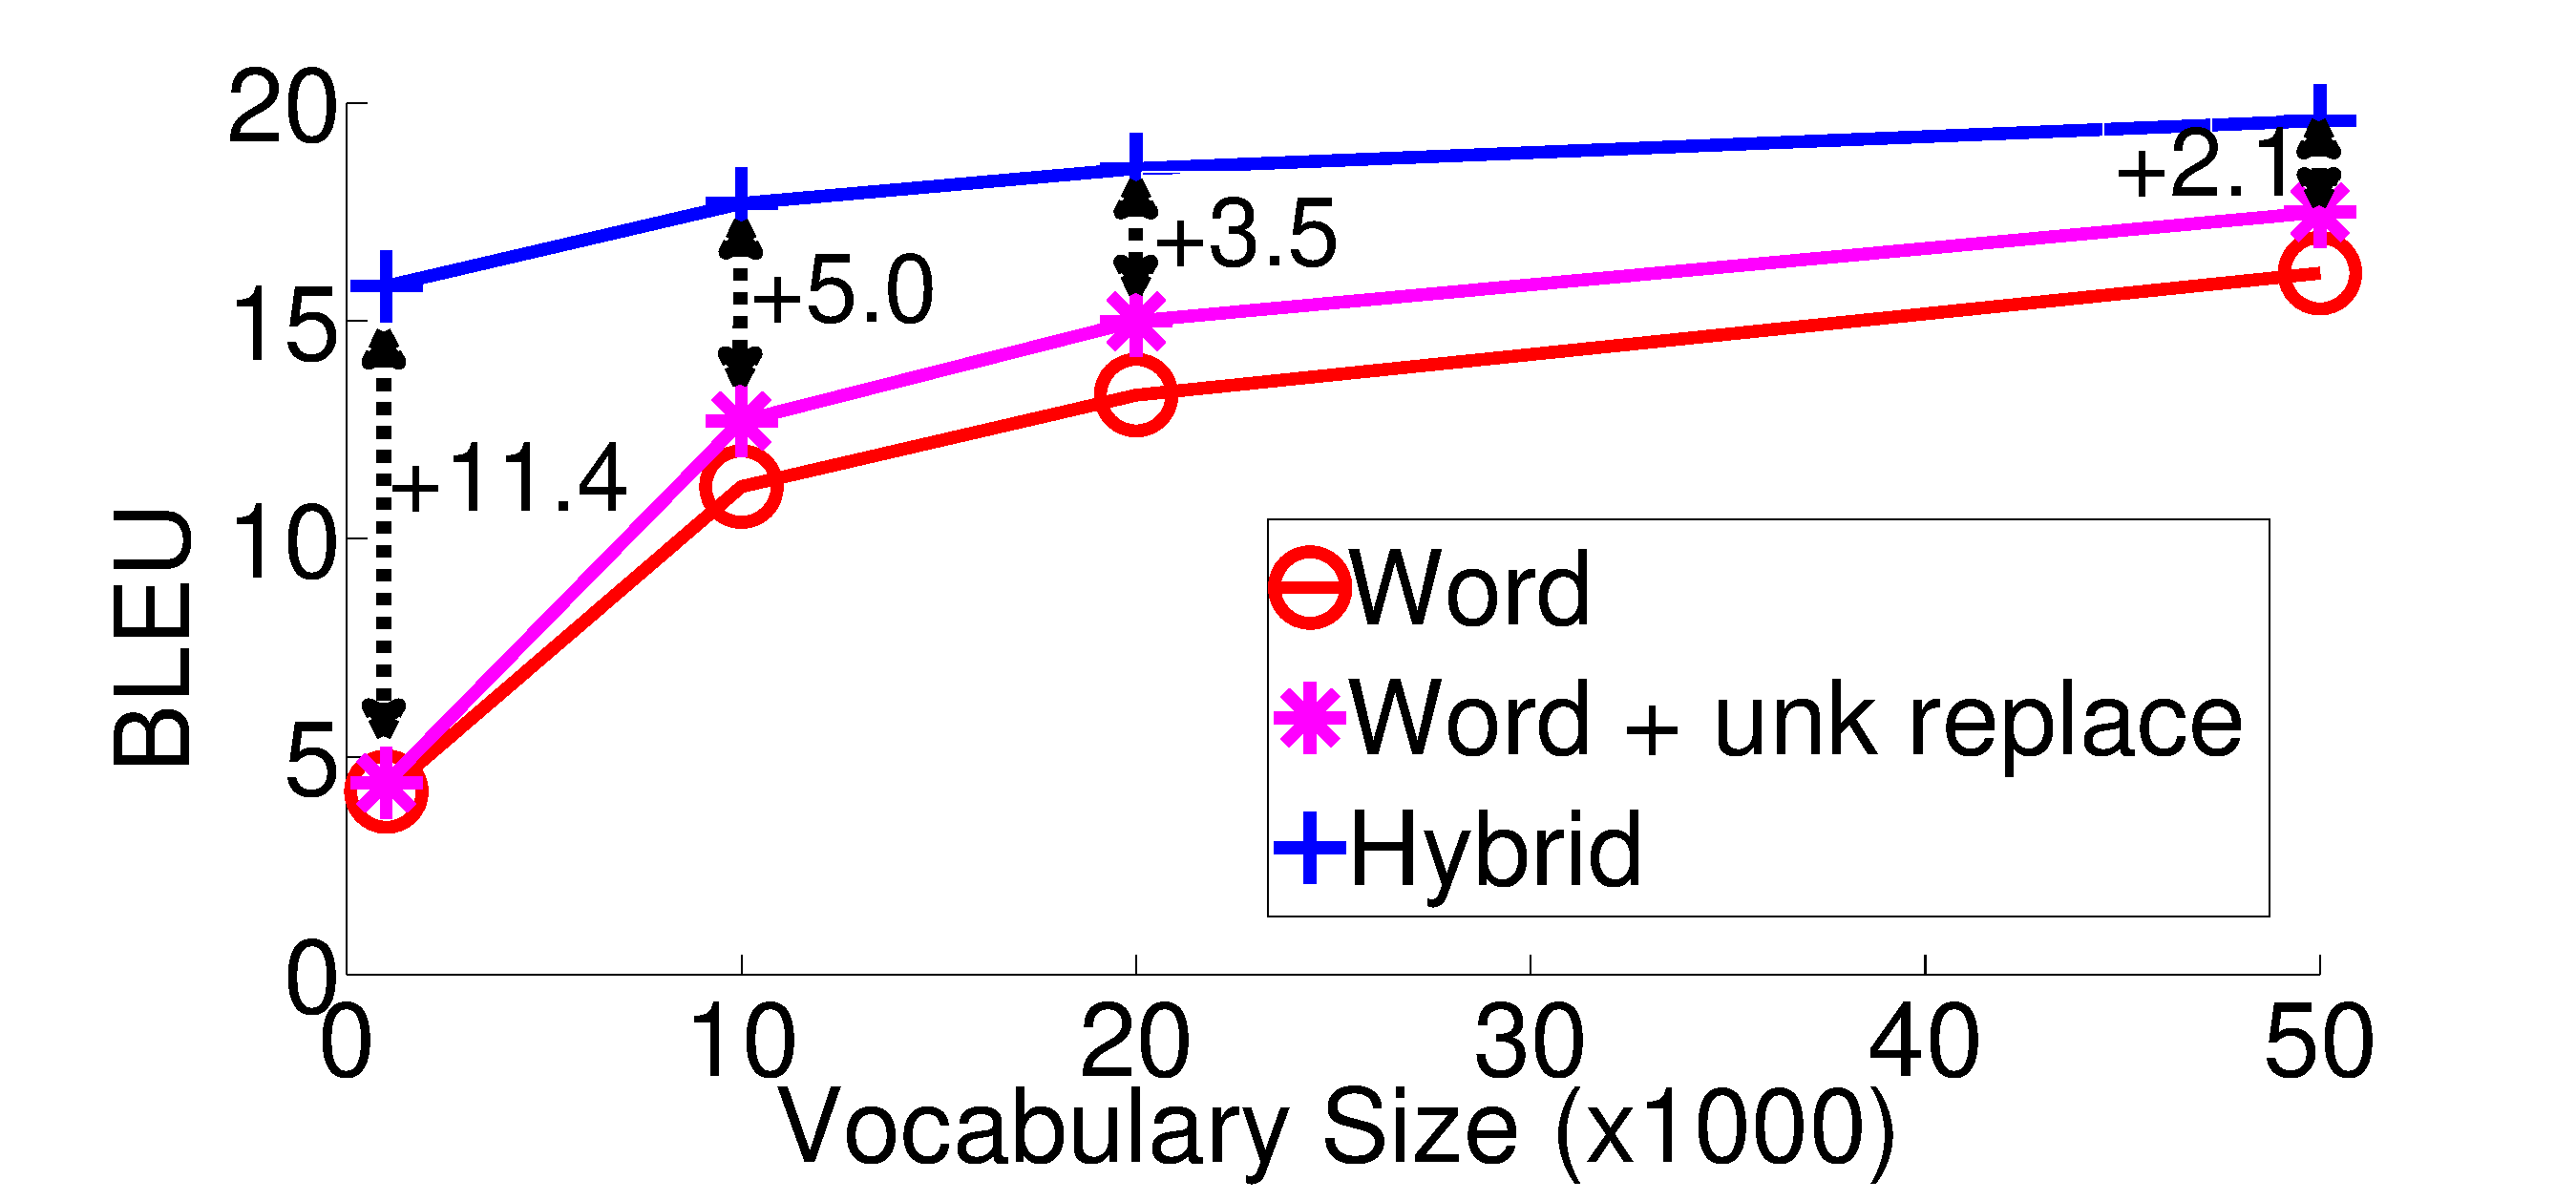
\includegraphics[width=0.7\textwidth, clip=true, trim= 0 0 0 0]{img/5-vocab}
\caption[Vocabulary size effect]{{\bf Vocabulary size effect} -- shown are the performances of different
systems as I vary their vocabulary sizes. I highlight the improvements obtained
by my hybrid models over word-based systems which already handle unknown words.}
\label{f:vocab}
\end{figure}



\subsection{Rare Word Embeddings}
I evaluate the {\it source} character-level model by building representations
for rare words and measuring how good these embeddings are.

Quantitatively, I follow \newcite{luong13} in using the word similarity task,
specifically on the {\it Rare Word} dataset, to judge the learned representations for
complex words. The evaluation metric is the Spearman's correlation $\rho$
between similarity scores assigned by a model and by human annotators.
From the results in Table~\ref{t:word_sim}, I can see that source representations produced by
my hybrid\footnote{I look up the encoder embeddings for frequent words and build representations for
rare word from characters.}  models
are significantly better than those of the word-based one. It is noteworthy that my deep recurrent
character-level models can outperform the model of \cite{luong13}, which uses
recursive neural networks and requires a complex morphological analyzer, by a large
margin. My performance is also competitive to the best Glove embeddings
\cite{pennington2014} which were trained on a much larger dataset.
\begin{table}[tbh!]
\centering
%\resizebox{8cm}{!}{
\begin{tabular}{c|l|c|c|c}
\multicolumn{2}{c|}{{\bf System}} & Size & $|V|$ & \bf{$\rho$}\\ %Spearman's 
  \hline
\multicolumn{2}{l|}{\cite{luong13}} & 1B & 138K & 34.4 \\
  \hdashline
\multicolumn{2}{l|}{\multirow{2}{*}{Glove \cite{pennington2014}}} & 6B & 400K & 38.1 \\
\multicolumn{2}{l|}{} & 42B & 400K & \bf{47.8} \\
  \hline
\multicolumn{4}{c}{{\it My NMT models}}\\
  \hline
\modelword{} & Word-based & 0.3B & 50K & 20.4 \\
  \hdashline
\modelsmall{} & Hybrid & 0.3B & 10K & 42.4 \\
  \hdashline
\model{} & Hybrid & 0.3B & 50K & \biformat{47.1} \\
\end{tabular}
%}
\caption[Word similarity task]{{\bf Word similarity task} -- shown are Spearman's correlation
$\rho$ on the {\it Rare Word} dataset
of various models (with different vocab sizes $|V|$). 
} 
\label{t:word_sim}
\end{table}


Qualitatively, I visualize embeddings produced by the hybrid model \model{} for
selected words in the Rare Word dataset.
Figure~\ref{f:visual} shows the two-dimensional representations of words
computed by the
Barnes-Hut-SNE algorithm \cite{bhsne}.\footnote{I run Barnes-Hut-SNE algorithm
over a set of 91 words, but filter out 27 words for displaying clarity.} It is extremely interesting to observe that
words are clustered together not only by the word structures but also by
the meanings. For example, in the top-left box,
the {\it character}-based representations for \word{loveless}, \word{spiritless}, \word{heartlessly}, and \word{heartlessness} are nearby,
but clearly separated into two groups. Similarly, in the center boxes, {\it
word}-based embeddings of
\word{acceptable}, \word{satisfactory}, \word{unacceptable}, and \word{unsatisfactory}, are
close by but separated by meanings. Lastly, the remaining boxes demonstrate that my
character-level models are able to build representations comparable to the
word-based ones, e.g., \word{impossibilities} vs.\ \word{impossible} and \word{antagonize}
vs.\ \word{antagonist}. All of this evidence strongly supports that the source
character-level models are useful and effective.

\begin{figure*}
\centering
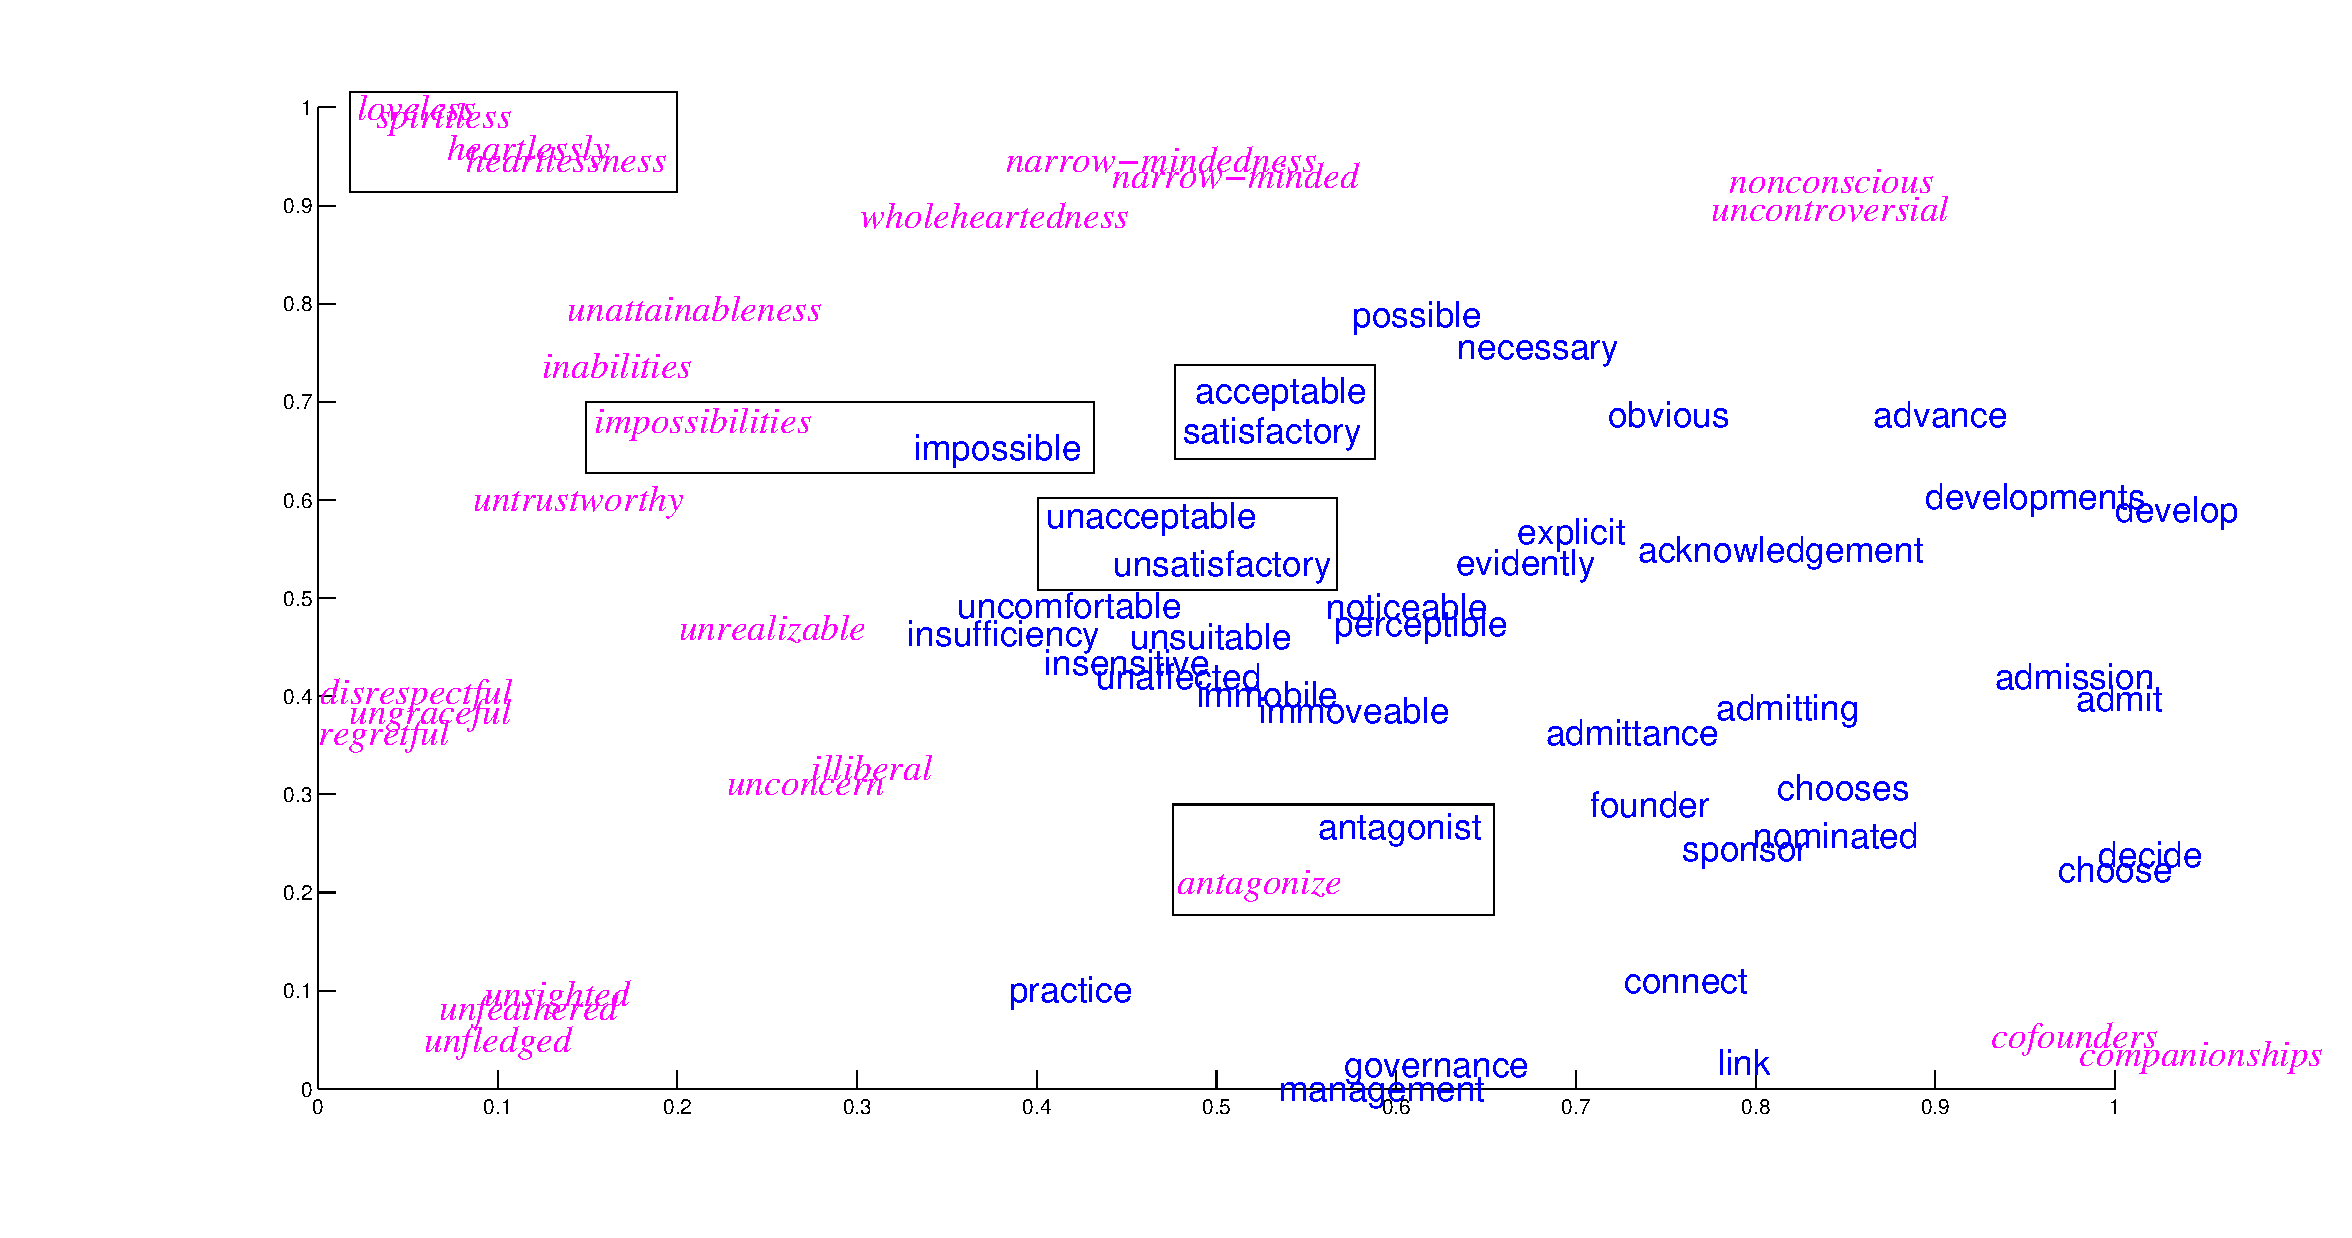
\includegraphics[width=\textwidth, clip=true, trim= 100 50 0 20]{img/5-emb}
\caption[Barnes-Hut-SNE visualization of source word representations]{{\bf Barnes-Hut-SNE visualization of source word representations} --
shown are sample words from the {\it Rare Word} dataset. I differentiate two types of
embeddings: {\color{blue} frequent} words in which encoder embeddings are looked up directly and {\it {\color{magenta} rare}} words
where I build representations from characters. Boxes highlight examples that
I will discuss in the text. I use the hybrid model \model{} in this visualization.}
\label{f:visual}
\end{figure*}


\begin{table*}%[tbh!]
\centering
\resizebox{15cm}{!}{
\begin{tabular}{c|c|p{15.5cm}}
% sent 1046 
\multirow{7}{*}{1} & source & The author \source{Stephen Jay Gould} died 20 years after
\source{diagnosis} . \\
& human & Autor \correct{Stephen Jay Gould} zem\u{r}el 20 let po
\correct{diagn\'oze} . \\
  \cline{2-3}
& \multirow{2}{*}{\it{word}} & Autor Stephen Jay \unk{} zem\u{r}el 20 let po
\unk{} . \\
&  & Autor \correct{Stephen Jay Gould} zem\u{r}el 20 let po \wrong{po} .\\
  \cline{2-3}
& \it{char} & Autor \wrong{Stepher Stepher} zem\u{r}el 20 let po
\correct{diagn\'oze} . \\
  \cline{2-3}
& \multirow{2}{*}{\it{hybrid}} & Autor \unk{} \unk{} \unk{} zem\u{r}el 20 let po
\unk{}. \\
&  & Autor \correct{Stephen Jay Gould} zem\u{r}el 20 let po \correct{diagn\'oze} .\\
  \hline
  \hline
% sent 80
\multirow{7}{*}{2} & source & As the Reverend \source{Martin Luther King
Jr.} said \source{fifty years ago} :\\
& human & Jak \correct{p\u{r}ed pades\'ati lety} \u{r}ekl reverend \correct{Martin
Luther King Jr} . : \\
  \cline{2-3}
& \multirow{2}{*}{\it{word}} & Jak \u{r}ekl reverend Martin \unk{} King \unk{}
p\u{r}ed pades\'ati lety : \\
&  & Jak \u{r}ekl reverend \correct{Martin Luther King} \wrong{\u{r}ekl}
\close{p\u{r}ed pades\'ati lety} : \\
  \cline{2-3}
& \it{char} & Jako reverend \correct{Martin Luther} \wrong{kr\'al \u{r}\'ikal}
\close{p\u{r}ed pades\'ati lety} : \\
  \cline{2-3}
& \multirow{2}{*}{\it{hybrid}} & Jak p\u{r}ed \unk{} lety \u{r}ekl \unk{} Martin
\unk{} \unk{} \unk{} : \\
&  & Jak \correct{p\u{r}ed pades\'ati lety} \u{r}ekl reverend \correct{Martin
Luther King} \close{Jr.} : \\
  \hline
  \hline
% sent 198
\multirow{7}{*}{3} & source & Her \source{11-year-old} daughter , \source{Shani Bart} , said it felt a " little bit
\source{weird} " [..] back to school \\
& human & Jej\'{i} \correct{jeden\'{a}ctilet\'{a}} dcera \correct{Shani Bartov\'{a}} prozradila
, \u{z}e " je to trochu \correct{zvl\'{a}\u{s}tn\'{i}} " [..] znova do
\u{s}koly \\
  \cline{2-3}
& \multirow{2}{*}{\it{word}} & Jej\'i \unk{} dcera \unk{} \unk{} \u{r}ekla , \u{z}e je to " trochu
divn\'e " , [..] vrac\'i do \u{s}koly \\
&  & Jej\'i \wrong{11-year-old} dcera \correct{Shani} \wrong{,} \u{r}ekla , \u{z}e je to " trochu
\close{divn\'e} " , [..] vrac\'i do \u{s}koly \\
  \cline{2-3}
& \it{char} & Jej\'i \correct{jeden\'actilet\'a} dcera , \correct{Shani
Bartov\'a} , \u{r}\'ikala ,
\u{z}e c\'it\'i trochu \close{divn\u{e}} , [..] vr\'atila do \u{s}koly \\
  \cline{2-3}
& \multirow{2}{*}{\it{hybrid}} & Jej\'i \unk{} dcera , \unk{} \unk{} , \u{r}ekla , \u{z}e c\'it\'i " trochu
\unk{} " , [..] vr\'atila do \u{s}koly \\
&  & Jej\'i \correct{jeden\'actilet\'a} dcera , \wrong{Graham} \close{Bart} , \u{r}ekla , \u{z}e c\'it\'i " trochu
\close{divn\'y} " , [..] vr\'atila do \u{s}koly \\
\end{tabular}
}
\caption[Sample translations on newstest2015]{{\bf Sample translations on newstest2015} -- %examples in both translation directions.
for each example, I show the {\it source}, {\it human} translation, and
translations of the following NMT systems: {\it word} model \modelword{},
{\it char} model \modelchar{}, and {\it hybrid} model \modelsmall{}. I show the
translations before replacing \unk{} tokens (if any) for the word-based 
and hybrid models. The following formats are used to highlight
\correct{correct}, \wrong{wrong}, and \close{close} translation segments.}
\label{t:sample}
\end{table*}


\subsection{Sample Translations}
\label{subsec:samples}

I show in Table~\ref{t:sample} sample translations between various systems. 
In the first example, my hybrid model translates perfectly. The word-based
model fails to translate \word{diagnosis} because the second \unk{} was incorrectly
aligned to the word \word{after}. The character-based model, on the other hand,
makes a mistake in translating names.

For the second example, the hybrid model surprises us when it can capture
the long-distance reordering of \word{fifty years ago} and \word{p\u{r}ed
pades\'ati lety} while the other two models do not. The word-based model
translates \word{Jr.} inaccurately due to the incorrect alignment between the
second \unk{} and the word \word{said}. The
character-based model literally translates the name \word{King} into \word{kr\'al}
which means \word{king}.

Lastly, both the character-based and hybrid models impress us by
their ability to translate compound words exactly, e.g., \word{11-year-old} and
\word{jeden\'actilet\'a}; whereas the identity copy
strategy of the word-based model fails.
Of course, my hybrid model does make mistakes, e.g., it fails to translate the name
\word{Shani Bart}. 
Overall, these examples highlight how challenging translating
into Czech is and that being able to translate at the character level helps
improve the quality.

\section{Conclusion}
\label{sec:conclude}
I have proposed a novel {\it hybrid} architecture that combines the strength
of both word- and character-based models. Word-level models are fast to train
and offer high-quality translation; whereas, character-level models help achieve
the goal of open vocabulary NMT. 
I have demonstrated these two aspects through my experimental results and
translation examples.

My best hybrid model has surpassed the performance of both the best word-based
NMT system and the best non-neural model to establish a new state-of-the-art result for 
English-Czech translation in WMT'15 with $\ensbleu{}$ BLEU.
Moreover, I have succeeded in replacing the standard unk replacement technique
in NMT with my character-level components, yielding an improvement of 
+$\gain{}$ BLEU points. My analysis has shown that my model has the ability to
not only generate well-formed words for
Czech, a highly inflected language with an enormous and complex vocabulary, but
also build accurate representations for English source words.
Additionally, I have demonstrated the potential of purely character-based
models in producing good translations;
they have outperformed past word-level NMT models. 
I will further discuss the potential of these models in Chapter~\ref{c:conclude}.


\chapter{The Future of NMT}
\label{c:future}
In previous chapters, my effort to improving neural machine
translation has centered around enhancing the model architecture to address
different needs such as translating long sentences or coping with
complex vocabularies. In this chapter, I switch gear to examine more ``external''
aspects of NMT, which is also a way for me to take a quick peek into the future of NMT.
Specifically, I first examine in Section~\ref{sec:multi-task} how NMT can be improved by utilizing data from
not only the translation but also other tasks such as parsing, image caption
generation, and unsupervised learning. This is framed under the {\it multi-task}
setting which I believe is important for NMT future given a humongous amount of
data available in the world growing at an exponentially fast pace. The second
aspect that I examine is on making NMT models smaller, a topic of 
increasing importance as mobile devices become dominant. Specifically, in
Section~\ref{sec:nmt-compression}, I cast such
desiderata as a {\it model compression} problem in which I answer how much we can
reduce the sizes of NMT models without sacrifice in performance and reveal
interesting patterns in the parameter space of NMT. Lastly, in
Section~\ref{sec:outlook}, I highlight other future trends and potential
research directions for NMT.


\section{Multi-task Sequence to Sequence Learning}
\label{sec:multi-task}
Multi-task learning (MTL) is an important machine learning paradigm that
aims at improving the generalization performance of a task using other related
tasks. 
Such framework has been widely studied by
\citet{thrun96,caruana97,evgeniou04,ando05,argyriou07,kumar12}, among many
others. In the context of deep neural networks, MTL has
been applied successfully to various problems ranging from language
\citep{liu15}, to vision
\citep{donahue14},
and speech \citep{heigold13,huang2013cross}.

Recently, sequence to sequence (\ssl{}) learning, proposed by
\citet{kal13}, \citet{sutskever14}, and \citet{cho14}, emerges as an effective paradigm for dealing with
variable-length inputs and outputs. \ssl{} learning, at its core, uses
recurrent neural networks to map variable-length input sequences to
variable-length output sequences.  While relatively new, the \ssl{}
approach has achieved state-of-the-art results in not only its original
application -- machine translation --
\citep{luong15,jean15,luong15attn,jean15wmt,luong15iwslt}, but also image caption generation \citep{vinyals15caption},
and constituency parsing \citep{vinyals15grammar}. 

Despite the popularity of multi-task learning and sequence to sequence
learning, there has been little work in combining MTL with \ssl{}
learning. To the best of our knowledge, there is only one recent
publication by \citet{dong15} which applies a \ssl{} models for machine
translation, where the goal is to translate from one language to
multiple languages.
In this work, we propose three MTL
approaches that complement one another: (a) the {\it \otm} approach -- for
tasks that can have an encoder in common, such as translation and parsing; this 
applies to the multi-target translation setting in \citep{dong15} as well, (b)
the {\it \mto} approach -- useful for multi-source
translation or tasks in which only the decoder can be easily shared,
such as translation and image captioning, and lastly, (c) the {\it \mtm} approach -- which share
multiple encoders and decoders through which we study the effect of unsupervised
learning in translation.
We show
that syntactic parsing and image caption generation improves the
translation quality between English and German by up to +$1.5$ BLEU points over
strong single-task baselines on the WMT benchmarks. 
Furthermore, we have established a new {\it state-of-the-art} result in
constituent parsing with 93.0 F$_1$.
We also explore two unsupervised learning
objectives, sequence autoencoders \citep{dai15} and skip-thought vectors
\citep{kiros15skip}, and reveal their interesting properties in the MTL setting: autoencoder helps less in terms of
  perplexities but more on BLEU scores compared to skip-thought.
%Our novel findings reveal that the skip-thought objective improves
%translation while the sequence autoencoders does not.


\subsection{Multi-task Sequence-to-Sequence Learning}
\label{subsec:multi}
I generalize the work of \citet{dong15} to the multi-task sequence-to-sequence
learning setting that includes the tasks of machine translation (MT),
constituency parsing, and image caption generation. Depending on which tasks 
are involved, I propose to categorize multi-task \ssl{} learning into three general
settings.
In addition, I will discuss the unsupervised learning tasks considered as well
as the learning process.

\paragraph{One-to-Many Setting}
%\label{subsec:otm}
This scheme involves {\it one encoder} and {\it multiple decoders} for tasks in
which the encoder can be shared, as illustrated in
Figure~\ref{f:otm}. The input to each task is a sequence of
English words. A separate decoder is used to generate each sequence of
output units which can be either (a) a sequence of tags for
constituency parsing as used in \citep{vinyals15grammar}, (b) a
sequence of German words for machine translation \citep{luong15attn},
and (c) the same sequence of English words for autoencoders or a
related sequence of English words for the skip-thought objective
\citep{kiros15skip}.

\begin{figure}[tbh]
\centering
%\psgrid
%\rput(7.5,2.6){$\alpha_1=1.0$}
%\rput(7.5,1.5){$\alpha_2=0.1$}
%\rput(7.5,0.4){$\alpha_3=0.5$}
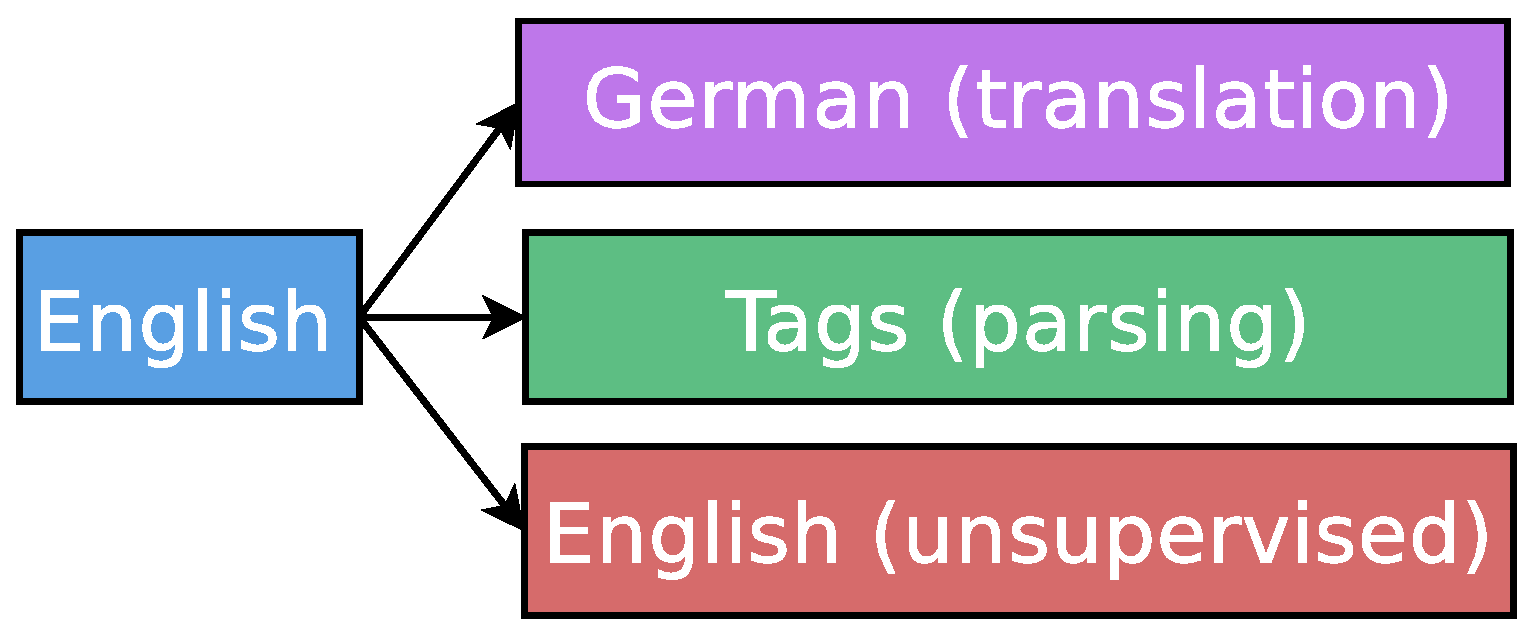
\includegraphics[width=0.45\textwidth, clip=true, trim= 0 0 0
0]{img/6-1_otm}
\caption[One-to-many Setting]{{\bf One-to-many Setting} -- one encoder, multiple decoders. This scheme
is useful for either multi-target translation as
in \cite{dong15} or between different tasks. Here, English and
German imply sequences of words in the respective languages. 
%The $\alpha$ values
%give the proportions of parameter updates that are allocated for the different tasks.
} 
\label{f:otm}
\end{figure}

\paragraph{Many-to-One Setting}
%\label{subsec:mto}
This scheme is the opposite of the {\it one-to-many}
setting. As illustrated in Figure~\ref{f:mto}, it consists of {\it multiple
encoders} and {\it one decoder}. This is useful for tasks in which only the
decoder can be shared, for example, when my tasks include machine translation
and image caption generation \citep{vinyals15caption}. In addition, from a machine
translation perspective, this setting can benefit from a large
amount of monolingual data on the target side, which is a standard
practice in machine translation system and has also been explored
for neural MT by \cite{gulcehre2015using}.

\begin{figure}[tbh]
\centering
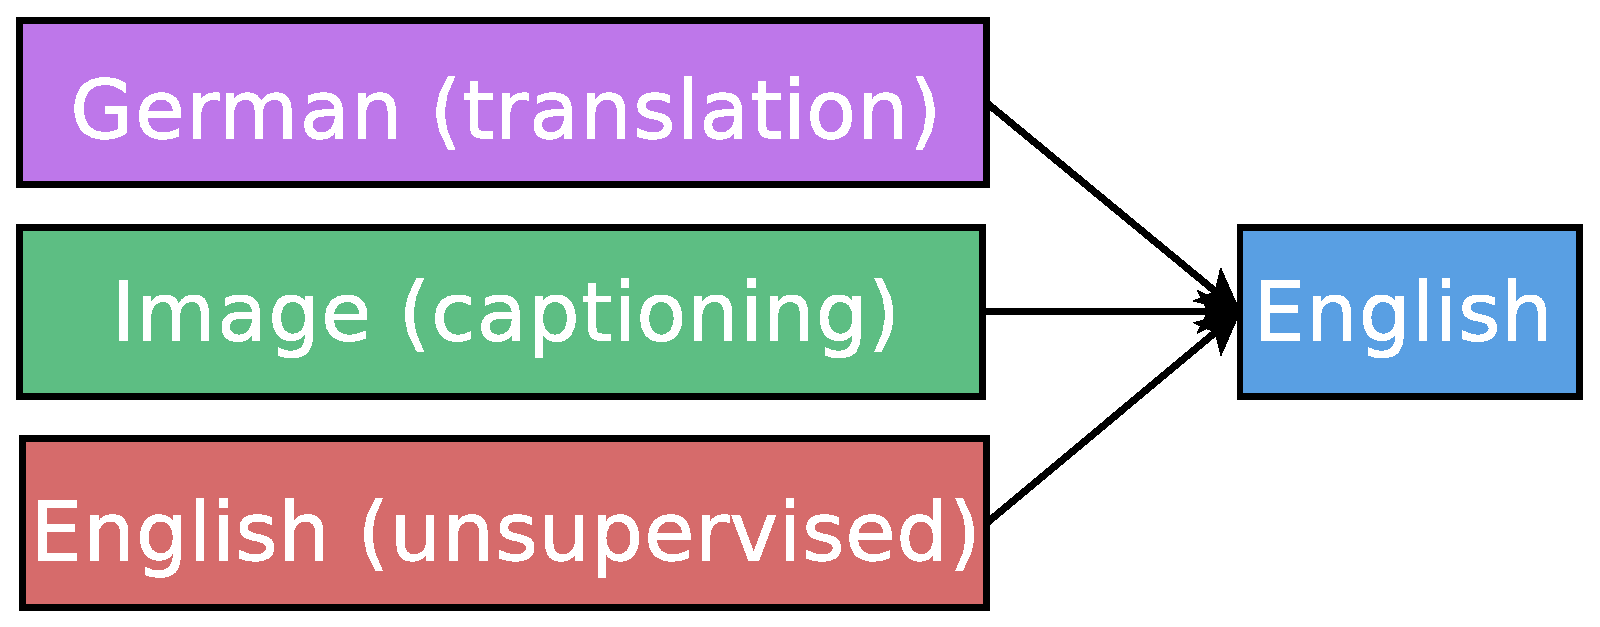
\includegraphics[width=0.5\textwidth, clip=true, trim= 0 0 0
0]{img/6-1_mto}
\caption[Many-to-one setting]{{\bf Many-to-one setting} -- multiple encoders, one decoder. This scheme
is handy for tasks in which only the decoders can be shared.}
\label{f:mto}
\end{figure}

\paragraph{Many-to-Many Setting}
%\label{subsec:mtm}
Lastly, as the name describes, this category is the most general one,
consisting of multiple encoders and multiple decoders.
%However, such
%flexibility also makes it difficult to determine which tasks should
%share which components. ---- Is it true? IS. 
%To simplify sharing, I consider a special use
%case in machine translation which involves two encoders and two
%decoders shared over three tasks.
I will explore this scheme in a translation setting that involves sharing multiple
encoders and multiple decoders.  In addition to the machine
translation task, I will include two unsupervised 
objectives over the source and target languages as illustrated in
Figure~\ref{f:mtm}.

\begin{figure}[tbh]
\centering
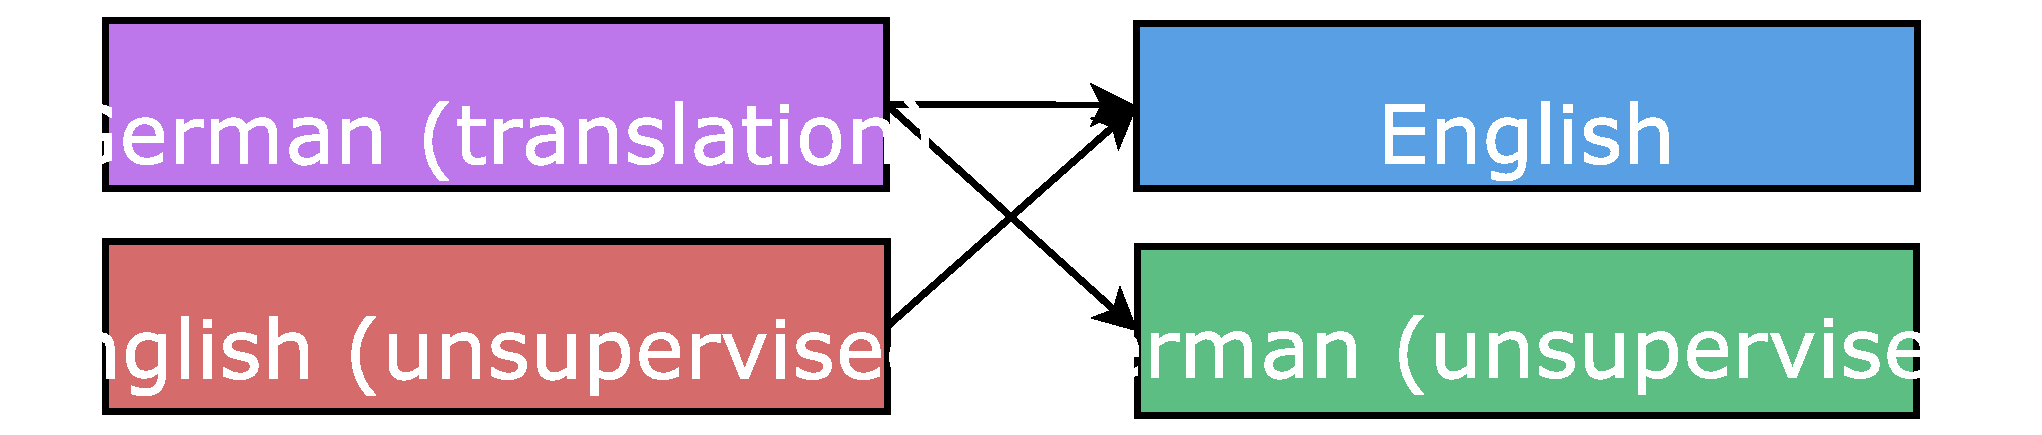
\includegraphics[width=0.7\textwidth, clip=true, trim= 0 0 0
0]{img/6-1_mtm}
\caption[Many-to-many setting]{{\bf Many-to-many setting} -- multiple encoders, multiple decoders. I
consider this scheme in a limited context of machine translation to utilize the large
monolingual corpora in both the source and the target languages. Here, I
consider a single translation task and two unsupervised autoencoder tasks.} 
\label{f:mtm}
\end{figure}

\paragraph{Unsupervised Learning Tasks}

My very first unsupervised learning task involves learning {\it autoencoders} from
monolingual corpora, which has recently been applied to sequence to sequence
learning \citep{dai15}. However, in \citet{dai15}'s work, the authors
only experiment with pretraining and then finetuning, but not joint training which
can be viewed as a form of multi-task learning (MTL). As such, I am 
very interested in knowing whether the same trend extends to my MTL settings.

Additionally, I investigate the use of the {\it skip-thought}
vectors \citep{kiros15skip} in the context of my MTL framework.
Skip-thought vectors are trained by training sequence to sequence
models on pairs of consecutive sentences, which makes the skip-thought
objective a natural \ssl{} learning candidate. A minor technical
difficulty with the skip-thought objective is that 
the training data must consist of ordered sentences, e.g., paragraphs.  Unfortunately, in
many applications that include machine translation, I only have
sentence-level data where the sentences are unordered. To
address that, I split each sentence into two halves; I then use 
one half to predict the other half.

\paragraph{Learning}
%\label{subsec:learning}
\cite{dong15} adopted an {\it alternating} training approach, where they
optimize each task for a fixed number of parameter updates (or
mini-batches) before switching to the next task (which is a different
language pair). In my setting, my tasks are more diverse and contain
different amounts of training data. As a result, I allocate different
numbers of parameter updates for each task, which are expressed with
the {\it mixing} ratio values $\alpha_i$ (for each task $i$). Each
parameter update consists of training data from one task only. When
switching between tasks, I select randomly a new task $i$ with
probability $\frac{\alpha_i}{\sum_j \alpha_j}$.
%{\bf [Thang, make sure that it is correct]} 


My convention is that the first task is the
{\it reference} task with $\alpha_1 = 1.0$ and the number of training
parameter updates for that task is prespecified to be $N$. A typical task $i$ will then be
trained for $\frac{\alpha_i}{\alpha_1}\cdot N$ parameter updates.
Such convention makes it easier for us to fairly compare the same reference
task in a single-task setting which has also been trained for exactly $N$
parameter updates.
When sharing an encoder or a decoder, I share both the recurrent connections
and the corresponding embeddings.

%This ensures
%fairness when comparing the performance of the reference task trained
%alone using the same number of mini-batches.
%IS:  I don't think that it follows.




\subsection{Experiments}
\label{sec:6_1_exp}
We evaluate the multi-task learning setup on a wide variety of
sequence-to-sequence tasks: constituency parsing, image caption
generation, machine translation, and a number of unsupervised learning as
summarized in Table~\ref{t:tasks}.

\subsection{Data}
\label{subsec:data}
Our experiments are centered around the {\it translation} task, where we aim to determine 
whether other tasks can improve translation and vice versa. We use the WMT'15 data
\citep{bojar15} for the English$\leftrightarrows$German
translation problem. Following 
\citet{luong15attn}, we use the 50K most frequent words for each
language from the training corpus.\footnote{The corpus has already been tokenized using the default
tokenizer from Moses.  Words not in these vocabularies are represented by the token
\texttt{<unk>}.} These vocabularies are then shared with other tasks, except for
parsing in which the target ``language'' has a vocabulary of 104 tags. 
We use newstest2013 (3000 sentences) as a validation set to select our
hyperparameters, e.g., mixing coefficients. For testing, to be comparable with existing results in
\citep{luong15attn}, we use the filtered
newstest2014 (2737
sentences)\footnote{\url{http://statmt.org/wmt14/test-filtered.tgz}} for the
English$\rightarrow$German translation task and newstest2015 (2169
sentences)\footnote{\url{http://statmt.org/wmt15/test.tgz}}
for the German$\rightarrow$English task.
See the summary in Table~\ref{t:tasks}.

For the {\it unsupervised} tasks, we use the English and German monolingual corpora
from WMT'15.\footnote{The training sizes reported for
the unsupervised tasks are
only 10\% of
the original WMT'15 monolingual corpora which we randomly sample from. Such reduced sizes are
for faster training time and already about three times larger than that of the parallel
data. We consider using all the monolingual data in future work.} Since in
our experiments, unsupervised tasks are always coupled with translation tasks,
we use the same validation and test sets as the accompanied translation tasks.

For {\it constituency parsing}, we experiment with two types of corpora:
\begin{enumerate}
\item a small corpus -- the widely used
Penn Tree Bank (PTB) dataset \citep{Marcus:1993:BLA} and,
\item a large corpus -- the high-confidence (HC) parse trees 
provided by \citet{vinyals15grammar}.
\end{enumerate}
The two parsing tasks, however, are evaluated on the same validation (section
22) and test (section 23)
sets from the PTB data. Note also that the parse trees have been linearized
following \citet{vinyals15grammar}. 
Lastly, for {\it image caption generation}, we use a dataset of image and caption pairs provided by
\citet{vinyals15caption}.


% together with various training details.
%\citep{vinyals15caption}\citep{luong15attn}\citep{dai15,kiros15skip}
\subsection{Training Details}

In all experiments, following \citet{sutskever14} and \citet{luong15}, we train deep LSTM
models as follows: (a) we use 4 LSTM layers each of which has
1000-dimensional cells and embeddings,\footnote{For image caption generation, we use 1024
dimensions, which is also the size of the image embeddings.} (b) parameters are
uniformly initialized in [-0.06, 0.06], (c) we use a mini-batch size of 128, (d)
dropout is applied with probability of 0.2 over vertical connections
\citep{pham2014dropout}, (e) we use SGD with a fixed
learning rate of 0.7, (f) input sequences are reversed, and lastly, (g) we use a simple finetuning schedule -- after $x$
epochs, we halve the learning rate every $y$ epochs. The values $x$ and $y$
are referred as {\it finetune start} and {\it finetune cycle} in
Table~\ref{t:tasks} together with the number of training epochs per task.

As described in Section~\ref{sec:multi}, for each multi-task
experiment, we need to choose one task to be the {\it reference
task} (which corresponds to $\alpha_1 = 1$). The choice of the
reference task helps specify the number of training epochs and the
finetune start/cycle values which we also when training that reference
task alone for fair comparison. To make sure our findings are
reliable, we run each experimental configuration twice and
report the average performance in the format {\it mean (stddev)}.

\begin{table}%[tbh!]
\centering
\resizebox{14cm}{!}{
\begin{tabular}{l|c|c|c|c|c|c|c|c}
\multirow{ 2}{*}{\bf{Task}} & {\bf Train} & {\bf Valid} &{\bf Test} &
\multicolumn{2}{c|}{{\bf Vocab Size}} & {\bf Train} &
\multicolumn{2}{c}{{\bf Finetune}}\\
  \cline{5-6} \cline{8-9}
  & {\bf Size}& {\bf Size}& {\bf Size} & Source & Target & {\bf Epoch} & Start & Cycle \\
  \hline
English$\rightarrow$German Translation & 4.5M & 3000 & 3003 & 50K & 50K & 12 & 8 & 1 \\
  \hline
German$\rightarrow$English Translation & 4.5M & 3000 & 2169 & 50K & 50K & 12 & 8 & 1 \\
  \hline
English unsupervised & 12.1M & \multicolumn{2}{c|}{\multirow{2}{*}{Details in
text}} & 50K & 50K & 6 & 4 & 0.5 \\
  \cline{1-2} \cline{5-9}
German unsupervised & 13.8M & \multicolumn{2}{c|}{} & 50K & 50K & 6 & 4 & 0.5 \\
  \hline
Penn Tree Bank Parsing & 40K & 1700 & 2416 & 50K & 104 & 40 & 20 & 4 \\
  \hline
High-Confidence Corpus Parsing & 11.0M & 1700 & 2416 & 50K & 104 & 6 & 4 & 0.5 \\
  \hline
Image Captioning & 596K & 4115 & -  & - & 50K & 10 & 5 & 1 \\ 
\end{tabular}
}
\caption{{\bf Data \& Training Details} -- Information about the different
datasets used in this work. For each task, we display the following
statistics: (a) the number of training examples, (b) the sizes of the
vocabulary, (c) the number of training epochs, and (d) details on when
and how frequent we halve the learning rates ({\it finetuning}).}
\label{t:tasks} 
\end{table}

\subsection{Results}
We explore several multi-task learning scenarios by combining a {\it
large} task (machine translation) with: (a) a {\it small} task -- Penn
Tree Bank (PTB) parsing, (b) a {\it medium-sized} task -- image
caption generation, (c) another {\it large} task -- parsing on the
high-confidence (HC) corpus, and (d) lastly, {\it unsupervised tasks},
such as autoencoders and skip-thought vectors. In terms of evaluation metrics,
we report both validation and test perplexities for all tasks. Additionally, we
also compute test BLEU scores \citep{Papineni02bleu} for the translation task.

\subsubsection{Large Tasks with Small Tasks} % -- {\it translation \& parsing}}
\label{subsubsec:big_small}

In this setting, we want to understand if a small task such as {\it
PTB parsing} can help improve the performance of a large task such as
translation.  Since the parsing task maps from a sequence of English
words to a sequence of parsing tags \citep{vinyals15grammar}, only the
encoder can be shared with an English$\rightarrow$German translation
task.  As a result, this is a {\it one-to-many}
MTL scenario ($\S$\ref{subsec:otm}).

To our surprise, the results in Table~\ref{t:big_small} suggest that
by adding a very small number of parsing mini-batches (with mixing ratio $0.01$,
i.e., one parsing mini-batch per 100 translation mini-batches), we can improve
the translation quality substantially. More concretely,
our best multi-task model yields a gain of +$1.5$ BLEU points over the
single-task baseline. It is worth pointing out that as shown in
Table~\ref{t:big_small}, our single-task baseline is very strong, even better
than the equivalent non-attention model reported in \citep{luong15attn}. Larger
mixing coefficients, however, overfit the small
PTB corpus; hence, achieve smaller gains in translation quality. 

For parsing, as \citet{vinyals15grammar} have shown that attention is crucial to
achieve good parsing performance when training on the small PTB corpus,
we do not set a high bar for our attention-free systems in this setup (better
performances are reported in Section~\ref{subsub:ll}). Nevertheless, the parsing
results in Table~\ref{t:big_small} indicate that MTL is
also beneficial for parsing, yielding an improvement of up to +$8.9$ F$_1$ points
over the baseline.\footnote{While perplexities correlate well with BLEU scores as shown
in \citep{luong15}, we observe empirically in Section~\ref{subsub:ll} that parsing perplexities are only
reliable if it is less than $1.3$. Hence, we omit parsing perplexities in
Table~\ref{t:big_small} for
clarity. The parsing test perplexities (averaged over two
runs) for the last four rows in Table~\ref{t:big_small} are 1.95, 3.05, 2.14, and 1.66. Valid perplexities
are similar.} 
It would be interesting to study how MTL can be
useful with the presence of the {\it attention} mechanism, which we
leave for future work.


\begin{table}[tbh!]
\centering
%\resizebox{14cm}{!}{
\begin{tabular}{l|c|c|c|c}
\multirow{ 2}{*}{\bf{Task}} & \multicolumn{3}{c|}{{\bf Translation}} &
\multicolumn{1}{c}{{\bf
Parsing}}\\
  \cline{2-5}
  & Valid ppl & Test ppl & Test BLEU & Test F$_1$ \\
  \hline
\citep{luong15attn} & - & 8.1 & 14.0 & -  \\
  \hline
\multicolumn{5}{c}{{\it Our single-task systems}} \\
  \hline
Translation & 8.8 (0.3) & 8.3 (0.2) & 14.3 (0.3) & -\\
  \hline
PTB Parsing & - & - & - & 43.3 (1.7) \\
  \hline
\multicolumn{5}{c}{{\it Our multi-task systems}} \\
  \hline
{\it Translation} + PTB Parsing (1x) &  8.5 (0.0) & 8.2 (0.0) & 14.7 (0.1) & 54.5 (0.4) \\
  \hline
{\it Translation} + PTB Parsing (0.1x) &  8.3 (0.1) & 7.9 (0.0) & 15.1 (0.0) &
{\bf 55.2 (0.0)}\\
  \hline
{\it Translation} + PTB Parsing (0.01x) &  {\bf 8.2} (0.2) & {\bf 7.7} (0.2) & {\bf
15.8} (0.4) & 39.8 (2.7) \\
\end{tabular}
%}
\caption{{\bf English$\rightarrow$German WMT'14 translation \& Penn Tree Bank parsing results} --
shown are perplexities (ppl), BLEU scores, and parsing F$_1$ for various systems. For muli-task
models, {\it reference} tasks are in
italic with the mixing ratio in parentheses. Our results are averaged over two
runs
in the format {\it mean (stddev)}. Best results are
highlighted in boldface.}
\label{t:big_small}
\end{table}

\subsubsection{Large Tasks With Medium Tasks} % -- {\it translation \& captioning}}
We investigate whether the same pattern carries over to a medium task
such as {\it image caption generation}. Since the image caption
generation task maps images to a sequence of
English words \citep{vinyals15caption,xu15}, only the decoder can be
shared with a German$\rightarrow$English translation task. Hence, this
setting falls under the {\it many-to-one} MTL setting ($\S$\ref{subsec:mto}).

The results in Table~\ref{t:big_medium} show the same trend we observed
before, that is, by training on another task for a very small
fraction of time, the model improves its performance on its main task.
Specifically, with 5 parameter updates for image caption generation per 100
updates for translation (so the mixing ratio of $0.05$), we obtain a 
gain of +$0.7$ BLEU scores over a strong single-task baseline. Our baseline is
almost a BLEU point better than the equivalent non-attention model reported in
\cite{luong15attn}.
%When the {\it reference} task is image caption generation, MTL is still
%useful.\footnote{See
%Section~\ref{subsec:learning} on the use of reference tasks for fair
%comparison.} For every captioning parameter update, if the model also performs
%MTL with 2 translation minibatches (a mixing ratio of $2$), a gain of +$3.3$ points in
%terms of image caption generation perplexity can be achieved.

\begin{table}[tbh!]
\centering
%\resizebox{14cm}{!}{
\begin{tabular}{l|c|c|c|c}
\multirow{ 2}{*}{\bf{Task}} & \multicolumn{3}{c|}{{\bf Translation}} &
\multicolumn{1}{c}{{\bf
Captioning}}\\
  \cline{2-5}
  & Valid ppl & Test ppl & Test BLEU & Valid ppl \\ % & Test ppl \\
  \hline
\citep{luong15attn} & - & 14.3 & 16.9 & - \\ %& - \\
  \hline
\multicolumn{5}{c}{{\it Our single-task systems}} \\
  \hline
Translation & 11.0 (0.0) & 12.5 (0.2) & 17.8 (0.1) & - \\ %& - \\
  \hline
Captioning & - & - & - & 30.8 (1.3) \\ % & \\
%Captioning (2 layer) & - & 29.4 (0.3) \\
%Captioning (1 layer) & - & 28.4 (0.1) \\
  \hline
\multicolumn{5}{c}{{\it Our multi-task systems}} \\
  \hline
{\it Translation} + Captioning (1x) & 11.9 & 14.0 & 16.7 & 43.3 \\ % & 43.0 \\
{\it Translation} + Captioning (0.1x) &  10.5 (0.4) & 12.1 (0.4) & 18.0 (0.6) &
{\bf 28.4} (0.3) \\ %& {\bf 27.9} (0.2) \\
{\it Translation} + Captioning (0.05x) &  {\bf 10.3} (0.1) &  {\bf 11.8} (0.0) &
{\bf 18.5} (0.0) & 30.1 (0.3) \\ % & 29.8 (0.5)\\
{\it Translation} + Captioning (0.01x) &  10.6 (0.0) & 12.3 (0.1)& 18.1 (0.4) & 35.2 (1.4)
\\ % &  34.1 (1.4) \\
%  \hline
%{\it Captioning} + Translation (1x) & 25.6 & & & 30.2 & \\
%{\it Captioning} + Translation (2x) & 16.5 (1.2) & & & {\bf 27.5} (0.1) & \\
%{\it Captioning} + Translation (5x) & 12.0 (0.0) & & & 27.9 (0.0) & \\
\end{tabular}
%}
\caption{{\bf German$\rightarrow$English WMT'15 translation \& captioning results} -- shown are
perplexities (ppl) and BLEU scores 
for various tasks with similar format as
in Table~\ref{t:big_small}. {\it Reference} tasks are in italic with mixing
ratios in parentheses. The average results of 2 runs are in {\it
mean (stddev)} format.} %; others are for 1 run only.} 
%Note that the captioning tasks are trained and tested
%using the same English vocabulary as the translation tasks with 50K words.}
\label{t:big_medium}
\end{table}


\subsubsection{Large Tasks with Large Tasks}
\label{subsub:ll}
Our first set of experiments is almost the same as the one-to-many setting in
Section~\ref{subsubsec:big_small} which combines {\it translation}, as the reference
task, with parsing. The only difference is in terms of parsing data. Instead of using the
small Penn Tree Bank corpus, we consider a large parsing resource, the
high-confidence (HC) corpus, which is provided by \citet{vinyals15grammar}.
As highlighted in Table~\ref{t:big_big_translation}, the
trend is consistent; MTL helps boost translation quality by up
to +$0.9$ BLEU points. 
%For this case, it is expected that we do not
%get better parsing results since the multi-task model has seen very
%little parsing data compared to the single-task model.

\begin{table}[tbh!]
\centering
%\resizebox{14cm}{!}{
\begin{tabular}{l|c|c|c}
\multirow{ 2}{*}{\bf{Task}} & \multicolumn{3}{c}{{\bf Translation}}\\
  \cline{2-4}
  & Valid ppl & Test ppl & Test BLEU\\
  \hline
\citep{luong15attn} & - & 8.1 & 14.0 \\
  \hline
\multicolumn{4}{c}{{\it Our systems}} \\
  \hline
Translation & 8.8 (0.3) & 8.3 (0.2) & 14.3 (0.3)\\
  \hline
{\it Translation} + HC Parsing (1x) &  8.5 (0.0) & 8.1 (0.1) & 15.0 (0.6) \\
{\it Translation} + HC Parsing (0.1x) &  {\bf 8.2} (0.3) & {\bf 7.7} (0.2) &
{\bf 15.2} (0.6)\\
{\it Translation} + HC Parsing (0.05x) &  8.4 (0.0) & 8.0 (0.1) & 14.8 (0.2) \\
\end{tabular}
%}
\caption{{\bf English$\rightarrow$German WMT'14 translation} -- shown are
perplexities (ppl) and BLEU scores of various translation models. Our
multi-task systems combine translation and parsing on the
high-confidence corpus together. Mixing
ratios are in parentheses and the average results over 2 runs are in {\it
mean (stddev)} format. Best results are bolded.}
\label{t:big_big_translation}
\end{table}

The second set of experiments shifts the attention to {\it parsing} by having it as the reference task. 
We show in Table~\ref{t:big_big_parsing} results that combine parsing with
either (a) the English autoencoder task or (b) the English$\rightarrow$German
translation task. Our models are compared against the best attention-based systems in
\citep{vinyals15grammar}, including the state-of-the-art result of 92.8 F$_1$.

\begin{table}[tbh!]
\centering
%\resizebox{14cm}{!}{
\begin{tabular}{l|c|c}
\multirow{ 2}{*}{\bf{Task}}& \multicolumn{2}{c}{{\bf
Parsing}}\\
  \cline{2-3}
  & Valid ppl & Test F$_1$\\
  \hline
  \hline
LSTM+A \citep{vinyals15grammar} &  - & 92.5 \\
LSTM+A+E \citep{vinyals15grammar} & - & {\bf 92.8} \\
  \hline
\multicolumn{3}{c}{{\it Our systems}} \\
  \hline
HC Parsing & 1.12/1.12 & 92.2 (0.1) \\
  \hline
{\it HC Parsing} + Autoencoder (1x) & 1.12/1.12 & 92.1 (0.1) \\
{\it HC Parsing} + Autoencoder (0.1x) & 1.12/1.12 & 92.1 (0.1) \\
{\it HC Parsing} + Autoencoder (0.01x) & 1.12/1.13 & 92.0 (0.1) \\
  \hline
{\it HC Parsing} + Translation (1x) & 1.12/1.13 & 91.5 (0.2) \\
{\it HC Parsing} + Translation (0.1x) & 1.13/1.13 & 92.0 (0.2) \\
{\it HC Parsing} + Translation (0.05x) & {\bf 1.11/1.12} & {\bf 92.4 (0.1)} \\
{\it HC Parsing} + Translation (0.01x) & 1.12/1.12 & 92.2 (0.0) \\
  \hline
Ensemble of 6 multi-task systems & - & {\bf 93.0} \\
\end{tabular}
%}
\caption{{\bf Large-Corpus parsing results} -- shown are
perplexities (ppl) and F$_1$ scores 
for various parsing models. Mixing ratios are in parentheses and the average
results over 2 runs are in {\it mean (stddev)} format. We show the individual perplexities for all runs
due to small differences among them. For \citet{vinyals15grammar}'s parsing results, LSTM+A
represents a single LSTM with attention, whereas LSTM+A+E indicates an ensemble
of 5 systems. Important results are bolded.}
\label{t:big_big_parsing}
\end{table}


Before discussing the multi-task results, we note a few interesting
observations. First, very small parsing perplexities, close to 1.1, can be achieved with large
training data.\footnote{Training solely on the small Penn Tree Bank
corpus can only reduce the perplexity to at most $1.6$, as evidenced by poor
parsing results in Table~\ref{t:big_small}. At the same time, these parsing
perplexities are much smaller than
what can be achieved by a translation task. This is because parsing only has
$104$ tags in the target vocabulary compared to
$50$K words in the translation case. Note that $1.0$ is the theoretical
lower bound.}  
Second, our baseline system can obtain a very competitive F$_1$ score of
92.2, rivaling \citet{vinyals15grammar}'s systems. This is rather surprising
since our models do not use any attention mechanism. A closer look into these
models reveal that there seems to be an architectural difference:
\citet{vinyals15grammar} use 3-layer LSTM with 256 cells and
512-dimensional embeddings; whereas our models use 4-layer LSTM with 1000 cells and
1000-dimensional embeddings. This further supports findings in \citep{rafal16} that
larger networks matter for sequence models.

For the multi-task results, while autoencoder does not seem to help parsing,
translation does. At the mixing ratio of 0.05, we obtain a non-negligible boost of 0.2 F$_1$ 
over the baseline and with 92.4 F$_1$, our multi-task system is on par with the best single system reported in
\citep{vinyals15grammar}. Furthermore, by ensembling 6 different multi-task
models (trained with the translation task at mixing ratios of
0.1, 0.05, and 0.01), we are able to establish a new {\it state-of-the-art} result in
English constituent parsing with {\bf 93.0} F$_1$ score.

%\begin{table}[tbh!]
%\centering
%\resizebox{14cm}{!}{
%\begin{tabular}{l|c|c|c|c|c|c}
%\multirow{ 2}{*}{\bf{Task}} & \multicolumn{3}{c|}{{\bf Translation}} &
%\multicolumn{3}{c}{{\bf
%Parsing}}\\
%  \cline{2-7}
%  & Valid ppl & Test ppl & Test BLEU & Valid ppl & Test ppl & Test F$_1$\\
%  \hline
%\citep{luong15attn} & - & 8.1 & 14.0 & - & - & - \\
%  \hline
%LSTM+A \citep{vinyals15grammar} & - & - & - & - & - & 92.5 \\
%LSTM+A+E \citep{vinyals15grammar} & - & - & - & - & - & {\bf 92.8} \\
%  \hline
%\multicolumn{6}{c}{{\it Our single-task systems}} \\
%  \hline
%Translation & 8.8 (0.3) & 8.3 (0.2) & 14.3 (0.3) & - & - & - \\
%  \hline
%HC Parsing & - & - & - & 1.12/1.12& 1.12/1.12 & 92.2 (0.1) \\
%  \hline
%\multicolumn{6}{c}{{\it Our multi-task systems}} \\
%  \hline
%{\it Translation} + HC Parsing (1x) &  8.5 (0.0) & 8.1 (0.1) & 15.0 (0.6) &
%1.13/1.13 & 1.12/1.12 & - \\
%{\it Translation} + HC Parsing (0.1x) &  {\bf 8.2} (0.3) & {\bf 7.7} (0.2) &
%{\bf 15.2} (0.6) &  1.18/1.19 & 1.17/1.18 & -  \\
%{\it Translation} + HC Parsing (0.05x) &  8.4 (0.0) & 8.0 (0.1) &
%14.8 (0.2) &  1.24/1.24 & 1.22/1.23 & - \\
%  \hline
%{\it HC Parsing} + Translation (1x) & 8.4 (0.0) & 8.0 (0.1) & - & 1.12/1.13 &
%1.12/1.12 & 91.5 (0.2) \\
%{\it HC Parsing} + Translation (0.1x) & 21.2 (0.5) & 22.6 (0.6) & - & 1.13/1.13 & 1.12/1.12 & 92.0 (0.2) \\
%{\it HC Parsing} + Translation (0.05x) & 31.4 (0.4) & 34.1 (0.5) & - & {\bf
%1.11/1.12} & {\bf 1.11/1.12} & {\bf 92.4 (0.1)} \\
%\end{tabular}
%}
%\caption{{\bf English$\rightarrow$German WMT'14 translation \& Large-Corpus parsing results} -- shown are
%perplexities (ppl) and BLEU scores 
%for various tasks with similar format as
%in Table~\ref{t:big_small}. {\it Reference} tasks are in italic with mixing
%ratios in parentheses. The average results of 2 runs are in {\it
%mean (stddev)}. For parsing, we show the individual perplexities for all runs
%due to small differences. For \citet{vinyals15grammar}'s parsing results, LSTM+A
%represents a single LSTM with attention, whereas LSTM+A+E indicates an ensemble
%of 5 systems.}
%\label{t:big_big}
%\end{table}

\subsubsection{Multi-tasks and Unsupervised Learning}
Our main focus in this section is to determine whether unsupervised
learning can help improve translation. Specifically, we follow the {\it
many-to-many} approach described in Section~\ref{subsec:mtm} to couple
the German$\rightarrow$English translation task with two unsupervised learning
tasks on monolingual corpora, one per language.
The results in Tables~\ref{t:unsupervised_de_en} show a similar trend as before,
a small amount of other tasks, in this case the {\it autoencoder} objective with
mixing coefficient 0.05, improves the translation quality by +$0.5$ BLEU
scores. However, as we train more on the 
autoencoder task, i.e. with larger mixing ratios, the translation performance gets worse. 

\begin{table}[tbh!]
\centering
\resizebox{14cm}{!}{
\begin{tabular}{l|c|c|c|c|c}
\multirow{ 2}{*}{\bf{Task}} & \multicolumn{3}{c|}{{\bf Translation}} &
\multicolumn{1}{c|}{{\bf
German}}& \multicolumn{1}{c}{{\bf English}}\\
  \cline{2-6}
  & Valid ppl & Test ppl & Test BLEU & Test ppl & Test ppl \\
  \hline
\citep{luong15attn} & - & 14.3 & 16.9 & - & -  \\
  \hline
\multicolumn{6}{c}{{\it Our single-task systems}} \\
  \hline
Translation & 11.0 (0.0) & 12.5 (0.2) & 17.8 (0.1) & - & - \\
  \hline
\multicolumn{6}{c}{{\it Our multi-task systems with Autoencoders}}\\
  \hline
{\it Translation} + autoencoders (1.0x) &  12.3 &  13.9 & 16.0 & {\bf 1.01} & 2.10 \\ % 1.04 & 2.75 \\
{\it Translation} + autoencoders (0.1x) & 11.4 & 12.7 & 17.7 & 1.13 & {\bf 1.44} \\ % 1.19 & 1.75 \\
{\it Translation} + autoencoders (0.05x) & {\bf 10.9} (0.1) & {\bf 12.0} (0.0) &
{\bf 18.3} (0.4) & 1.40 (0.01) & 2.38 (0.39) \\
%{\it Translation} + autoencoders (2.0x) &  10.1 &  {\bf 1.05} & {\bf 1.04} \\
  \hline
\multicolumn{6}{c}{{\it Our multi-task systems with Skip-thought Vectors}}\\
  \hline
{\it Translation} + skip-thought (1x) & {\bf 10.4} (0.1) & {\bf 10.8} (0.1) & 17.3
(0.2) & {\bf 36.9} (0.1) & {\bf 31.5} (0.4) \\ %39.0 (0.2) & 38.1 (0.1) \\
{\it Translation} + skip-thought (0.1x) &  10.7 (0.0) & 11.4 (0.2) & 17.8 (0.4)
& 52.8 (0.3) & 53.7 (0.4) \\ %  51.0 (0.2) & 64.2 (0.4)\\
{\it Translation} + skip-thought (0.01x) &  11.0 (0.1) & 12.2 (0.0) & {\bf
17.8} (0.3)
& 76.3 (0.8) & 142.4 (2.7) \\ % 69.5 (0.4) & 165.3 (3.6)\\
\end{tabular}
}
\caption{{\bf German$\rightarrow$English WMT'15 translation \& unsupervised learning results} -- shown are perplexities
for translation and unsupervised learning tasks. We experiment with both {\it
autoencoders} and {\it skip-thought vectors} for the unsupervised objectives. Numbers in {\it
mean (stddev)} format are the average results of 2 runs; others are for 1 run
only.}
%shown are perplexities
%for translation and unsupervised learning tasks. We follow the same format as in
%Table~\ref{t:unsupervised_en_de}.}
\label{t:unsupervised_de_en}
\end{table}

{\it Skip-thought} objectives, on the other hand, behave differently. If we
merely look at the perplexity metric, the results are very encouraging: with
more skip-thought data, we perform better consistently across both the
translation and the unsupervised tasks. However, when computing the BLEU scores,
the translation quality degrades as we increase the mixing coefficients. We anticipate that
this is due to the fact that the skip-thought objective changes the nature of
the translation task when using one half of a sentence to predict the other
half. It is not a problem for the autoencoder objectives, however, since one can
think of autoencoding a sentence as translating into the same language.

We believe these findings pose interesting challenges in the quest towards  better
unsupervised objectives, which should satisfy the following criteria: (a)
a desirable objective should be compatible with the supervised task in focus, e.g.,
autoencoders can be viewed as a special case of translation,
and (b) with more unsupervised data, both intrinsic and extrinsic metrics
should be improved; skip-thought objectives satisfy this criterion in terms of
the intrinsic metric but not the extrinsic one.

%results with {\it
%skip-thought} objectives which improve translation performance between
%English and German in both directions. In addition, we observe
%that better translation perplexities are achieved as we increase
%the portions of unsupervised parameter updates from 
%$0.01$ to $1$. These results show that the skip-thought objective
%is better than the autoencoder as an unsupervised objective for language tasks.

%As a side note, we observe that the source-to-source unsupervised tasks
%($3^{\text{rd}}$ column) seem to benefit this MTL setting more than the
%target-to-target unsupervised tasks ($4^{\text{th}}$ column). This might be
%explained by the asymmetric structure in the sequence to sequence learning framework
%\citep{sutskever14} that no prediction is made on the source side {\bf [To thang: I don't understand
%this last point]}.

%\begin{table}[tbh!]
%\centering
%%\resizebox{8cm}{!}{
%\begin{tabular}{l|c|c|c}
%\multirow{ 2}{*}{\bf{Task}} & \multicolumn{3}{c}{{\bf Perplexity}}\\
%  \cline{2-4}
%  & Translation & English & German \\
%  \hline
%Translation& 8.8 (0.3) & - & -\\
%  \hline
%\multicolumn{4}{c}{{\it Autoencoders}}\\
%  \hline
%{\it Translation} + autoencoders (0.1x) & 9.0 &  1.37 & 3.85 \\
%{\it Translation} + autoencoders (1.0x) &  10.0 &  1.09 & 2.78 \\
%%{\it Translation} + autoencoders (2.0x) &  10.1 &  1.05 & 1.04 \\
%  \hline
%{\it Translation} + skip-thought (0.01x) & 8.6 (0.4)  & 64.1 (1.7) & 150.9
%(1.3) \\
%{\it Translation} + skip-thought (0.1x) &  8.8 (0.3) &  46.5 (0.5) & 72.7
%(9.1)\\
%{\it Translation} + skip-thought (1x) & {\bf 8.4} (0.2)  & 35.0 (0.6) &
%43.1 (1.5)\\
%\end{tabular}
%%}
%\caption{{\bf English$\rightarrow$German translation \& unsupervised learning results} -- shown are perplexities
%for translation and unsupervised learning tasks. We experiment with both {\it
%autoencoders} and {\it skip-thought vectors} for the unsupervised objectives. Numbers in {\it
%mean (stddev)} format are the average results of 2 runs; others are for 1 run
%only.}
%\label{t:unsupervised_en_de}
%\end{table}




\subsection{Conclusion}
\label{sec:conclude}

In this section, I showed that multi-task learning (MTL) can improve the
performance of the attention-free sequence to sequence model of
\citep{sutskever14}.  I found it surprising that training on syntactic
parsing and image caption data improved our translation performance, given
that these 
datasets are orders of magnitude smaller than typical translation
datasets. 
Furthermore, I have established a new {\it state-of-the-art} result in
constituent parsing with an ensemble of multi-task models.
I also showed that the two unsupervised
learning objectives, autoencoder and skip-thought, behave differently in the MTL context
involving translation. I hope that these interesting
findings will motivate future work in utilizing unsupervised data for sequence
to sequence learning.
A criticism of this work is that the sequence to sequence models do not employ
the attention mechanism \citep{bog15}.  I leave the exploration
of MTL with attention for future work.





\section{Compression of NMT Models via Pruning}
\label{sec:nmt-compression}
While NMT has a significantly smaller memory footprint than traditional phrase-based approaches (which need to store gigantic phrase-tables and
language models), the model size of NMT is still prohibitively large for mobile devices.
For example, the NMT system in Chapter 4 \cite{luong15attn}requires over 200 million
parameters, resulting in a storage size of hundreds of megabytes. 
Though the trend for bigger and deeper neural networks has brought great progress, it has also introduced over-parameterization, resulting in long running times, overfitting, and the storage size issue discussed above. 
A solution to the over-parameterization problem could potentially aid all three issues, though the first (long running times) is outside the scope of this work.

I investigate the efficacy of weight pruning for NMT as a means of compression.
I show that despite its simplicity, magnitude-based pruning with retraining is highly effective, and I compare three magnitude-based pruning schemes --- \textit{class-blind}, \textit{class-uniform} and \textit{class-distribution}.
Though recent work has chosen to use the latter two, I find the first and simplest scheme --- \textit{class-blind} --- the most successful.
I am able to prune 40\% of the weights of a state-of-the-art NMT system with negligible performance loss, and by adding a retraining phase after pruning, I can prune 80\% with no performance loss.
My pruning experiments also reveal some patterns in the distribution of
redundancy in NMT. In particular, I find that higher layers, attention and softmax weights are the most important, while lower layers and the embedding weights hold a lot of redundancy. 
For the Long Short-Term Memory (LSTM) architecture, I find that at lower layers the parameters for the input are most crucial, but at higher layers the parameters for the gates also become important.


\subsection{Related Work}
\label{subsec:related}
Pruning the parameters from a neural network, referred to as \textit{weight pruning} or \textit{network pruning}, is a well-established idea though it can be implemented in many ways. 
Among the most popular are the Optimal Brain Damage (OBD)
\cite{lecun1989optimal} and Optimal Brain Surgeon (OBS) \cite{hassibi1993second} techniques, which involve computing the Hessian matrix of the loss function with respect to the parameters, in order to assess the \textit{saliency} of each parameter. 
Parameters with low saliency are then pruned from the network and the remaining sparse network is retrained. 
Both OBD and OBS were shown to perform better than the so-called `naive magnitude-based approach', which prunes parameters according to their magnitude (deleting parameters close to zero).
However, the high computational complexity of OBD and OBS compare unfavorably to the computational simplicity of the magnitude-based approach, especially for large networks \cite{augasta2013pruning}.

In recent years, the deep learning renaissance has prompted a re-investigation of network pruning for modern models and tasks. 
Magnitude-based pruning with iterative retraining has yielded strong results for Convolutional Neural Networks (CNN) performing visual tasks.
\cite{collins2014memory} prune 75\% of AlexNet parameters with small accuracy loss on the ImageNet task, while \cite{han2015learning} prune 89\% of AlexNet parameters with no accuracy loss on the ImageNet task.

Other approaches focus on pruning neurons rather than parameters, via sparsity-inducing regularizers \cite{murray2015auto} or `wiring together' pairs of neurons with similar input weights \cite{srinivas2015data}. These approaches are much more constrained than weight-pruning schemes; they necessitate finding entire zero rows of weight matrices, or near-identical pairs of rows, in order to prune a single neuron. By contrast weight-pruning approaches allow weights to be pruned freely and independently of each other. The neuron-pruning approach of \cite{srinivas2015data} was shown to perform poorly (it suffered performance loss after removing only 35\% of AlexNet parameters) compared to the weight-pruning approach of \cite{han2015learning}. 
Though \cite{murray2015auto} demonstrates neuron-pruning for language modeling as part of a (non-neural) Machine Translation pipeline, their approach is more geared towards architecture selection than compression.

\begin{sloppypar}
There are many other compression techniques for neural networks, including approaches based on on low-rank approximations for weight matrices \cite{jaderberg2014speeding,denton2014exploiting}, or weight sharing  via hash functions \cite{chen2015compressing}.
Several methods involve reducing the precision of the weights or activations \cite{courbariaux2014low}, sometimes in conjunction with specialized hardware \cite{gupta2015deep}, or even using binary weights \cite{lin2015neural}.
The `knowledge distillation' technique of \cite{hinton2015distilling} involves training a small `student' network on the soft outputs of a large `teacher' network.
Some approaches use a sophisticated pipeline of several techniques to achieve impressive feats of compression \cite{han2015deep,iandola2016squeezenet}.
\end{sloppypar}

Most of the above work has focused on compressing CNNs for vision tasks. 
I extend the magnitude-based pruning approach of \cite{han2015learning} to recurrent neural networks (RNN), in particular LSTM architectures for NMT, and to my knowledge I am the first to do so.
There has been some recent work on compression for RNNs \cite{lu2016learning,prabhavalkar2016compression}, but it focuses on other, non-pruning compression techniques. 
Nonetheless, my general observations on the distribution of redundancy in a
LSTM, detailed in Section \ref{subsubsec:redundancy}, are corroborated by \cite{lu2016learning}.



\subsection{Our Approach}
\label{subsec:approach}
%We first give a brief overview of Neural Machine Translation before describing
%the model architecture of interest, the deep multi-layer recurrent model with
%LSTM. We then explain the different types of NMT weights
%together with our approaches to pruning and retraining.
%
%\subsection{Neural Machine Translation}
%Neural machine translation aims to directly model the conditional probability $p(\tgt{}|\src{})$ of translating
%a source sentence, $\src{1},\ldots,\src{n}$, to a target sentence, $\tgt{1},\ldots,\tgt{m}$.
%It accomplishes this goal through an {\it encoder-decoder} framework
%\cite{kal13,sutskever2014sequence,cho14}. The {\it encoder} computes a representation $\MB{s}$
%for each source sentence. Based on that source representation,
%the {\it decoder} generates a translation, one target word at a time, and hence,
%decomposes the log conditional probability as:
%\begin{equation}
%\log p(\tgt{}|\src{}) = \sum_{t=1}^m \nolimits \log
%p\open{\tgt{t}|\tgt{<t},\MB{s}}
%\label{e:s2s}
%\end{equation}
%
%Most NMT work uses RNNs, but approaches differ in terms of: 
%(a) architecture, which can be unidirectional, bidirectional, or deep multi-layer RNN; 
%and (b) RNN type, which can be Long Short-Term Memory (LSTM) \cite{hochreiter1997long} or the Gated Recurrent Unit \cite{cho14}. 

In this work, we specifically consider the {\it deep multi-layer recurrent} architecture with {\it
LSTM} as the hidden unit type.
Figure \ref{fig:nmt_simple} illustrates an instance of that architecture during training in which the source and target sentence pair are input for supervised
learning. During testing, the target sentence is not known in advance; instead, the most probable
target words predicted by the model are fed as inputs into the next timestep.
The network stops when it emits the end-of-sentence symbol --- a special `word' in the vocabulary, represented by a dash in Figure \ref{fig:nmt_simple}.


\subsubsection{Understanding NMT Weights}
\label{subsubsec:lstm}
Figure~\ref{fig:nmt_complex} shows the same system in more detail,
highlighting the different types of parameters, or weights, in the model.
We will go through the architecture from bottom to top.
First, a vocabulary is chosen for each language, assuming that the top $V$ frequent
words are selected.
Thus, every word in the source or target vocabulary can be represented by a one-hot vector of length $V$.
The source input sentence and target input sentence, represented as a sequence
of one-hot vectors, are transformed into a sequence of word embeddings by the
\emph{embedding} weights. 
These embedding weights, which are learned during training, are different for the source words and the target words.
The word embeddings and all hidden layers are vectors of length $n$ (a chosen hyperparameter).

The word embeddings are then fed as input into the main network, which consists
of two multi-layer RNNs `stuck together' --- an encoder for the source
language and a decoder for the target language, each with their own
weights. 
The \emph{feed-forward} (vertical) weights connect
the hidden unit from the layer below to the upper RNN block, and the
\emph{recurrent} (horizontal) weights connect the hidden unit from the previous
time-step RNN block to the current time-step RNN block.

The hidden state at the top layer of the decoder is fed through an
\textit{attention} layer, which guides the translation by `paying attention' to relevant parts of the source sentence; 
for more information see \cite{bahdanau2014neural} or Section 3 of \cite{luong2015effective}.
Finally, for each target word, the top layer hidden unit is transformed by the
\emph{softmax} weights into a score vector of length $V$. The target word with the highest score is selected as the output translation.

\bi{Weight Subgroups in LSTM} -- For the aforementioned RNN block, we choose to
use LSTM as the hidden unit type. To facilitate our later discussion 
on the different subgroups of weights
within LSTM, we first review the details of LSTM as formulated by 
\newcite{zaremba2014recurrent} as follows:
\begin{align}
\begin{pmatrix}
i\\
f\\
o\\
\hat{h}
\end{pmatrix}
&=
\begin{pmatrix}
\text{sigm}\\
\text{sigm}\\
\text{sigm}\\
\text{tanh}
\end{pmatrix}
T_{4n,2n}
\begin{pmatrix}
h_t^{l-1}\\
h_{t-1}^l
\end{pmatrix} \label{eqn:lstm_1} \\
c_t^l&=f \circ c_{t-1}^l + i \circ \hat{h} \label{eqn:lstm_2} \\
h_t^l &= o \circ \text{tanh}(c_t^l) \label{eqn:lstm_3}
\end{align}
Here, each LSTM block at time $t$ and layer $l$ computes as output a pair of
hidden and memory vectors ($h_t^l$, $c_t^l$) given the previous pair
($h_{t-1}^l$, $c_{t-1}^l$) and an input vector $h_t^{l-1}$ (either from the LSTM block below or
the embedding weights if $l\!=\!1$). All of these vectors
have length $n$.

The core of a LSTM block is the weight matrix $T_{4n,2n}$ of size $4n \times
2n$. This matrix can be decomposed into 8 subgroups that are responsible for the
interactions between $\{$input gate $i$, forget gate $f$, output gate $o$,
input signal $\hat{h}\} \times \{$feed-forward input $h_t^{l-1}$, recurrent
input $h_{t-1}^l\}$.

%\subsection{Evaluation metrics}
%We evaluate our models by two measures: BLEU score and perplexity. 
%BLEU compares the output target sentence with the human-translated target sentence, and is measured on a scale from 0 (worst) to 100 (best).
%Perplexity is the exponential of the average loss per word, measured on a scale from 1 (best) to infinity (worst). 
%%For each output target word, the model produces scores for each word in the vocabulary, which are converted to a probability distribution over the vocabulary. 
%The \emph{loss} is the negative log probability of the correct word --- that is, the lower the system's certainty in choosing the correct word, the higher the loss.
%
%Both evaluation metrics are valuable. 
%BLEU measures a system's performance on the end-goal of machine translation, translation quality, whereas perplexity is the quantity minimized during training.
%BLEU is a `hard' measure of performance, as it is calculated based on the sentences produced by the network, whereas perplexity is a `softer', more fine-grained measure that takes into account not just whether the correct target word was produced, but the probability of producing the correct target word.
%We use both BLEU and perplexity in this paper, as appropriate.

\subsubsection{Pruning Schemes}
\label{subsubsec:approach_schemes}
We follow the general magnitude-based approach of \cite{han2015learning}, which consists of pruning weights with smallest absolute value. However, we question the authors' pruning scheme with respect to the different weight classes, and experiment with three pruning schemes.
Suppose we wish to prune $x$\% of the total parameters in the model. 
How do we distribute the pruning over the different weight classes (illustrated in Figure~\ref{fig:nmt_complex}) of our model? 
We propose to examine three different pruning schemes:
\begin{enumerate}
\item \textit{Class-blind}: 
Take all parameters, sort them by magnitude and prune the $x$\% with smallest magnitude, regardless of weight class.
(So some classes are pruned proportionally more than others).
\item \textit{Class-uniform}: 
Within each class, sort the weights by magnitude and prune the $x$\% with smallest magnitude.
(So all classes have exactly $x$\% of their parameters pruned).
\item \textit{Class-distribution}: 
 For each class $c$, weights with magnitude less than $\lambda \sigma_c$ are
 pruned. Here, $\sigma_c$ is the standard deviation of that class and $\lambda$ is a universal parameter chosen such that in total, $x\%$ of all parameters are pruned.
This is used by \cite{han2015learning}.
\end{enumerate}
All these schemes have their seeming advantages.
Class-blind pruning is the simplest and adheres to the principle that pruning
weights (or equivalently, setting them to zero) is least damaging when
those weights are small, regardless of their locations in the architecture.
Class-uniform pruning and class-distribution pruning both seek to prune
proportionally within each weight class, either absolutely, or relative to the
standard deviation of that class.
We find that class-blind pruning outperforms both other schemes (see Section~\ref{subsec:exp_schemes}).

\subsubsection{Retraining}
\label{subsubsec:approach_retraining}
In order to prune NMT models aggressively without performance loss, we retrain our pruned networks. 
That is, we continue to train the remaining weights, but maintain the sparse structure introduced by pruning.
In our implementation, pruned weights are represented by zeros in the weight matrices, 
and we use binary `mask' matrices, which represent the sparse structure of a network, 
to ignore updates to weights at pruned locations.
This implementation has the advantage of simplicity as it requires minimal changes to the training and deployment code, 
but we note that a more complex implementation utilizing sparse matrices and sparse matrix multiplication could potentially yield speed improvements.
However, such an implementation is beyond the scope of this paper.




\subsection{Experiments}
\label{subsec:exp}
I evaluate the effectiveness of my pruning approaches on the attention-based English-German NMT system 
from Chapter 4 \cite{luong15attn}. 
Training data was obtained from WMT'14 consisting
of 4.5M sentence pairs (116M English words, 110M German words). For
more details on training hyperparameters, I refer readers to Section 4.1 of
the thesis.
All models are tested on newstest2014 (2737 sentences). 
The model achieves a
perplexity of 6.1 and a BLEU score of
20.5 (after unknown word replacement).\footnote{The performance of this model
is reported under row {\it global (dot)} in Table 4.1 of the thesis.}

When {\it retraining} pruned NMT systems, I use the following settings: (a) I start
with a smaller learning rate of 0.5 (the original model uses a learning rate of
1.0), (b) I train for fewer epochs, 4 instead of 12, using plain SGD, (c) a simple learning
rate schedule is employed; after 2 epochs, I begin to halve the learning rate
every half an epoch, and (d) all other hyperparameters are the same, such as
mini-batch size 128, maximum gradient norm 5, and dropout with probability 0.2.

\subsubsection{Comparing pruning schemes}
\label{subsubsec:exp_schemes}
Despite its simplicity, I observe in Figure~\ref{fig:pruning_methods} that {\it
class-blind} pruning outperforms both other schemes in terms of translation
quality at all pruning percentages.
In order to understand this result, for each of the three pruning schemes, I pruned each class separately and recorded the effect on performance (as measured by perplexity).
Figure \ref{fig:breakdown} shows that with class-uniform pruning, the overall performance loss is caused disproportionately by a few classes: target layer 4, attention and softmax weights. Looking at Figure \ref{fig:scatter}, I see that the most damaging classes to prune also tend to be those with weights of greater magnitude --- these classes have much larger weights than others at the same percentile, so pruning them under the class-uniform pruning scheme is more damaging. The situation is similar for class-distribution pruning.



By contrast, Figure \ref{fig:breakdown} shows that under class-blind pruning, the damage caused by pruning softmax, attention and target layer 4 weights is greatly decreased, and the contribution of each class towards the performance loss is overall more uniform.
In fact, the distribution begins to reflect the number of parameters in each class --- for example, the source and target embedding classes have larger contributions because they have more weights. 
I use only class-blind pruning for the rest of the experiments.

Figure \ref{fig:breakdown} also reveals some interesting information about the
distribution of redundancy in NMT architectures --- namely it seems that higher
layers are more important than lower layers, and that attention and softmax
weights are crucial. I will explore the distribution of redundancy further in
Section \ref{subsubsec:redundancy}.

\begin{figure}
\centering
% !TEX root = acl2016.tex

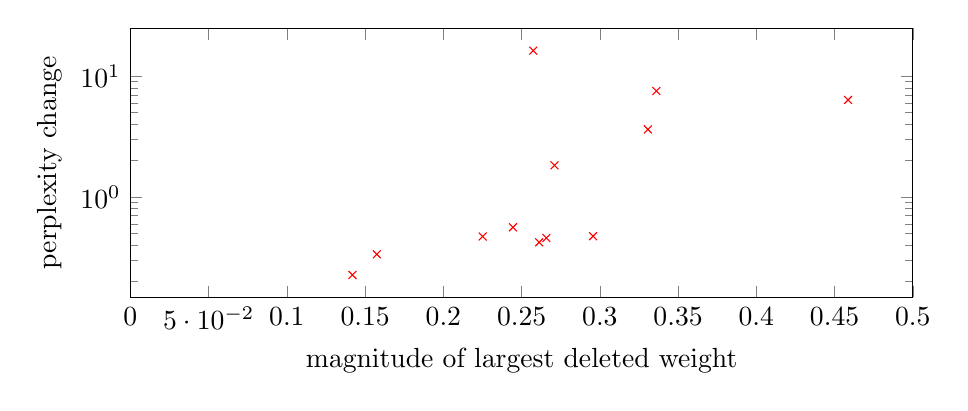
\begin{tikzpicture}
\begin{semilogyaxis}[
width=0.95\columnwidth,
height=5cm,
xlabel={magnitude of largest deleted weight}, 
ylabel={perplexity change},
xmin=0,
xmax=0.5,
]
\addplot[
only marks,
color=red,
mark=x,
]
table[row sep=crcr]
{
0.22513		0.471137\\
0.244492		0.561763\\
0.270999		1.829927\\
0.330704		3.628541\\
0.261247		0.422055\\
0.265832		0.457759\\
0.295644		0.473893\\
0.336088		7.545939\\
0.458583		6.362093\\
0.257479		16.277336\\
0.157486		0.335614\\
0.14194		0.226382\\
};
\end{semilogyaxis}
\end{tikzpicture}
\caption[Magnitude of largest deleted weight vs. perplexity change]{Magnitude of largest deleted weight vs. perplexity change, for the 12
different weight classes when pruning 90\% of parameters by class-uniform
pruning.}
\label{fig:scatter}
\end{figure}

\subsubsection{Pruning and retraining}
\label{subsec:effect}


Pruning has an immediate negative impact on performance (as measured by BLEU) that is exponential in pruning percentage; this is demonstrated by the blue line in Figure \ref{fig:main_results}.
However I find that up to about 40\% pruning, performance is mostly unaffected, indicating a large amount of redundancy and over-parameterization in NMT.

I now consider the effect of retraining pruned models.
The orange line in Figure \ref{fig:main_results} shows that after retraining the pruned models, baseline performance (20.48 BLEU) is both recovered and improved upon, up to 80\% pruning (20.91 BLEU), with only a small performance loss at 90\% pruning (20.13 BLEU).
This may seem surprising, as I might not expect a sparse model to significantly out-perform a model with five times as many parameters.
There are several possible explanations, two of which are given below.
\begin{figure}
\centering
% !TEX root = acl2016.tex

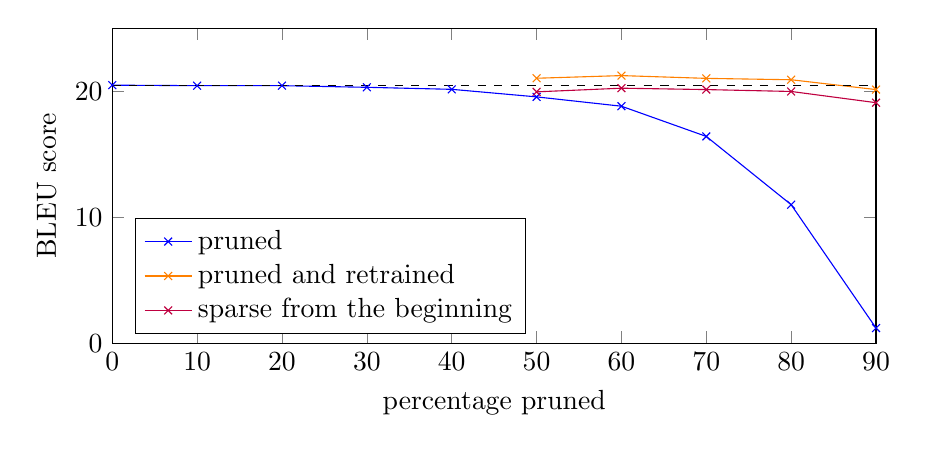
\begin{tikzpicture}

\begin{axis}[%
width=0.8\columnwidth,
height=4cm,
scale only axis,
xmin=0,
xmax=90,
xtick={0,10, 20, 30, 40, 50, 60, 70, 80, 90},
xlabel={percentage pruned},
ymin=0,
ymax=25,
yminorticks=true,
ylabel={BLEU score},
axis background/.style={fill=white},
legend pos = south west,
legend cell align=left,
]
\addplot [color=blue,solid,mark=x,mark options={solid}]
  table[row sep=crcr]{%
  0	20.48\\
10	20.44\\
20	20.44\\
30	20.31\\
40	20.15\\
50	19.55\\
60	18.81\\
70	16.41\\
80	10.99\\
90	1.2\\
};
\addlegendentry{pruned}

\addplot [color=orange,solid,mark=x,mark options={solid}]
  table[row sep=crcr]{%
50	21.03\\
60	21.24\\
70	21.02\\
80	20.91\\
90	20.13\\
};
\addlegendentry{pruned and retrained}

\addplot [color=purple,solid,mark=x,mark options={solid}]
  table[row sep=crcr]{%
50	19.95\\
60	20.24\\
70	20.13\\
80	19.98\\
90	19.09\\
};
\addlegendentry{sparse from the beginning}

\addplot [color=black,dashed]
  table[row sep=crcr]{%
0	20.48\\
90	20.48\\
};
\end{axis}
\end{tikzpicture}%
\caption[Performance of pruned models]{Performance of pruned models (a) after pruning, (b) after pruning and
retraining, and (c) when trained with sparsity structure from the outset (see
Section \ref{subsec:sparse}).}
\label{fig:main_results}
\end{figure}

Firstly, I found that the less-pruned models perform better on the training set than the validation set, whereas the more-pruned models have closer performance on the two sets. 
This indicates that pruning has a regularizing effect on the retraining phase, though clearly more is not always better, as the 50\% pruned and retrained model has better validation set performance than the 90\% pruned and retrained model.
Nonetheless, this regularization effect may explain why the pruned and retrained models outperform the baseline.
\begin{figure}[tbh]
\centering
% !TEX root = acl2016.tex

\begin{tikzpicture}

\begin{axis}[%
width=0.8\columnwidth,
height=4cm,
scale only axis,
xmin=0,
xmax=540000,
%xtick={},
xlabel={training iterations},
ymin=1,
ymax=8,
yminorticks=true,
ylabel={loss},
axis background/.style={fill=white},
%legend pos = south west,
%legend cell align=left
]

\addplot [color=black,dotted]
  table[row sep=crcr]{%
0	2.27\\
540000	2.27\\
};

\addplot [color=black,dotted]
  table[row sep=crcr]{%
405000	0\\
405000	8\\
};

\addplot [color=blue,solid,mark options={solid}]
  table[row sep=crcr]{%
5000	6.89\\
10000	5.91\\
15000	5.34\\
20000	4.88\\
25000	4.35\\
30000	3.9\\
35000	3.66\\
40000	3.61\\
45000	3.55\\
50000	3.5\\
55000	3.43\\
60000	3.3\\
65000	3.16\\
70000	3.07\\
75000	3.06\\
80000	3.05\\
85000	3.04\\
90000	3.01\\
95000	2.94\\
100000	2.86\\
105000	2.82\\
110000	2.82\\
115000	2.82\\
120000	2.81\\
125000	2.8\\
130000	2.75\\
135000	2.7\\
140000	2.67\\
145000	2.67\\
150000	2.67\\
155000	2.67\\
160000	2.66\\
165000	2.63\\
170000	2.59\\
175000	2.57\\
180000	2.57\\
185000	2.57\\
190000	2.57\\
195000	2.57\\
200000	2.54\\
205000	2.51\\
210000	2.5\\
215000	2.5\\
220000	2.5\\
225000	2.5\\
230000	2.5\\
235000	2.48\\
240000	2.45\\
245000	2.44\\
250000	2.44\\
255000	2.44\\
260000	2.44\\
265000	2.44\\
270000	2.42\\
275000	2.4\\
280000	2.39\\
285000	2.39\\
290000	2.4\\
295000	2.4\\
300000	2.4\\
305000	2.38\\
310000	2.36\\
315000	2.35\\
320000	2.35\\
325000	2.36\\
330000	2.36\\
335000	2.35\\
340000	2.34\\
345000	2.32\\
350000	2.31\\
355000	2.31\\
360000	2.31\\
365000	2.31\\
370000	2.31\\
375000	2.29\\
380000	2.28\\
385000	2.27\\
390000	2.27\\
395000	2.27\\
400000	2.27\\
405000	2.27\\
410000	2.53\\
415000	2.52\\
420000	2.48\\
425000	2.42\\
430000	2.22\\
435000	2.05\\
440000	1.99\\
445000	2.04\\
450000	2.08\\
455000	2.11\\
460000	2.12\\
465000	2.06\\
470000	1.99\\
475000	1.96\\
480000	1.99\\
485000	2.02\\
490000	2.03\\
495000	2.04\\
500000	2.01\\
505000	1.96\\
510000	1.95\\
515000	1.97\\
520000	1.98\\
525000	2\\
530000	2\\
535000	1.98\\
540000	1.95\\
};

\end{axis}
\end{tikzpicture}%
\caption[Validation set losses during training, pruning and retraining]{The validation set loss during training, pruning and retraining. The vertical dotted line marks the point when 80\% of the parameters are pruned. The horizontal dotted line marks the best performance of the unpruned baseline.}

\label{fig:loss_curve}
\end{figure}

\begin{figure*}
\centering
\includegraphics[width=\textwidth]{img/6-2_redundancy_good} %trim = 0mm 130mm 300mm 0mm, clip, 
\caption[Graphical representation of the location of small weights]{Graphical representation of the location of small weights in various parts of the model. 
Black pixels represent weights with absolute size in the bottom 80\%; white pixels represent those with absolute size in the top 20\%.
Equivalently, these pictures illustrate which parameters remain after pruning 80\% using my class-blind pruning scheme.
}
\label{fig:redundancy_location}
\end{figure*}



Alternatively, pruning may serve as a means to escape a local optimum. 
Figure \ref{fig:loss_curve} shows the loss function over time during the training, pruning and retraining process.
During the original training process, the loss curve flattens out and seems to converge (note that I use early stopping to obtain my baseline model, so the original model was trained for longer than shown in Figure \ref{fig:loss_curve}).
Pruning causes an immediate increase in the loss function, but enables further gradient descent, allowing the retraining process to find a new, better local optimum.
It seems that the disruption caused by pruning is beneficial in the long-run.

\subsubsection{Starting with sparse models}
\label{subsec:sparse}
The favorable performance of the pruned and retrained models raises the question: can I get a shortcut to this performance by \emph{starting} with sparse models?
That is, rather than train, prune, and retrain, what if I simply prune then train?
To test this, I took the sparsity structure of my 50\%--90\% pruned models, and trained completely new models with the same sparsity structure.
The purple line in Figure \ref{fig:main_results} shows that the `sparse from the beginning' models do not perform as well as the pruned and retrained models, but they do come close to the baseline performance.
This shows that while the sparsity structure alone contains useful information about redundancy and can therefore produce a competitive compressed model, it is important to interleave pruning with training.

Though my method involves just one pruning stage, other pruning methods interleave pruning with training more closely by including several iterations \cite{collins2014memory,han2015learning}.
I expect that implementing this for NMT would likely result in further compression and performance improvements.



\subsubsection{Storage size}
The original unpruned model (a MATLAB file) has size 782MB.
The 80\% pruned and retrained model is 272MB, which is a 65.2\% reduction.
In this work I focus on compression in terms of number of parameters rather than storage size, because it is invariant across implementations.

\subsubsection{Distribution of redundancy in NMT}
\label{subsubsec:redundancy}

I visualize in Figure~\ref{fig:redundancy_location} the redundancy structore of
my NMT baseline model.
{\it Black} pixels represent weights near to zero (those that can be pruned); {\it white} pixels represent larger ones.
First I consider the embedding weight matrices, whose columns correspond to words in the vocabulary.
Unsurprisingly, in Figure \ref{fig:redundancy_location}, I see that the parameters corresponding to the less common words are more dispensable.
In fact, at the 80\% pruning rate, for 100 uncommon source words and 1194
uncommon target words, I delete \emph{all} parameters corresponding to that word.
This is not quite the same as removing the word from the vocabulary --- true out-of-vocabulary words are mapped to the embedding for the `unknown word' symbol, whereas these `pruned-out' words are mapped to a zero embedding.
However in the original unpruned model these uncommon words already had near-zero embeddings, indicating that the model was unable to learn sufficiently distinctive representations.

Returning to Figure \ref{fig:redundancy_location}, now look at the eight weight matrices for the source and target connections at each of the four layers.
Each matrix corresponds to the $4n \times 2n$ matrix $T_{4n,2n}$ in Equation (\ref{eqn:lstm_1}).
In all eight matrices, I observe --- as does \cite{lu2016learning} --- that the weights connecting to the input $\hat{h}$ are most crucial, followed by the input gate $i$, then the output gate $o$, then the forget gate $f$. 
This is particularly true of the lower layers, which focus primarily on the input $\hat{h}$. 
However for higher layers, especially on the target side, weights connecting to the gates are as important as those connecting to the input $\hat{h}$.
The gates represent the LSTM's ability to add to, delete from or retrieve information from the memory cell.
Figure \ref{fig:redundancy_location} therefore shows that these sophisticated memory cell abilities are most important at the \emph{end} of the NMT pipeline (the top layer of the decoder).
This is reasonable, as I expect higher-level features to be learned later in a deep learning pipeline.

I also observe that for lower layers, the feed-forward input is much more important than the recurrent input, whereas for higher layers the recurrent input becomes more important.
This makes sense: lower layers concentrate on the low-level information from the current word embedding (the feed-forward input), whereas higher layers make use of the higher-level representation of the sentence so far (the recurrent input).

Lastly, on close inspection, I notice several white diagonals emerging within
some subsquares of the matrices in Figure \ref{fig:redundancy_location},
indicating that even without initializing the weights to identity matrices
(as is sometimes done \cite{le2015simple}),
an identity-like weight matrix is learned. At higher pruning percentages, these diagonals become more pronounced.

\subsection{Generalizability of my results}
To test the generalizability of my results, I also test my pruning approach
on a smaller, non-state-of-the-art NMT model trained on the WIT3 Vietnamese-English 
dataset \cite{iwslt15}, which consists of 133,000 sentence pairs.
This model is effectively a scaled-down version of the state-of-the-art model in Chapter 4 \cite{luong15attn},
with fewer layers, smaller vocabulary size, smaller hidden layer size, no attention mechanism,
and about 11\% as many parameters in total.
It achieves a BLEU score of 9.61 on the validation set.

Although this model and its training set are on a different scale to my main model, 
and the language pair is different, 
I found very similar results. 
For this model, it is possible to prune 60\% of parameters with no immediate performance loss,
and with retraining it is possible to prune 90\%, and regain original performance.
My main observations from Section \ref{subsubsec:exp_schemes} %to \ref{subsubsec:redundancy}
are also replicated; in particular, class-blind pruning is most successful,
`sparse from the beginning' models are less successful than pruned and retrained models,
and I observe the same patterns as seen in Figure \ref{fig:redundancy_location}.




\subsection{Conclusion}
\label{subsec:conclusion}
We have shown that weight pruning with retraining is a highly effective method of compression and regularization on a state-of-the-art NMT system, compressing the model to 20\% of its size with no loss of performance. 
Though we are the first to apply compression techniques to NMT, we obtain a similar degree of compression to other current work on compressing state-of-the-art deep neural networks, with an approach that is simpler than most.
We have found that the absolute size of parameters is of primary importance when choosing which to prune, leading to an approach that is extremely simple to implement, and can be applied to any neural network.
Lastly, we have gained insight into the distribution of redundancy in the NMT architecture.

In terms of future work, including \emph{several} iterations of pruning and retraining would likely improve the compression and performance of our pruning method.
If possible it would be highly valuable to exploit the sparsity of the pruned
models to speed up training and runtime, perhaps through sparse matrix
representations and multiplications (see Section \ref{subsubsec:approach_retraining}).
Though we have found magnitude-based pruning to perform very well, it would be instructive to revisit the original claim that other pruning methods (for example Optimal Brain Damage and Optimal Brain Surgery) are more principled, and perform a comparative study.




\section{Future Outlook}
\label{sec:outlook}
In this section, I will take the liberty to speculate on the future of NMT by first extending on ideas I have just discussed, multi-task learning and model compression. After that, I will talk about two other future trends on handling long context and new approaches to training sequence models beside maximum-likelihood estimation.\footnote{Some of the content of this section is based on the NMT tutorial that I, Kyunghuyn Cho, and Christopher D. Manning gave at ACL 2016 \url{https://sites.google.com/site/acl16nmt/}.}

\subsection{Multi-task and Semi/Un-supervised Learning}
In \secref{sec:multi-task}, I have assessed the feasibility of utilizing other tasks, such as parsing, image caption, and unsupervised learning, to improve translation. The positive gains in the translation quality that we achieved further reinforces my belief that multi-task learning is an important direction for the future of NMT (and even for Artificial General Intelligence). In the short-term future, as successors to our work, there have been fruitful results in building {\it multilingual} NMT systems \cite{zoph16,firat16,gnmt16multi,ha16} in which translations in multiple languages are viewed as different tasks. A nice by-product of such a system is the ability to do {\it zero-shot learning} which has been demonstrated convincingly by \newcite{gnmt16multi}. In that work, the authors built a single model that can do translation for 12 language pairs using the same sub-word vocabulary. Even more exciting, they can translate reasonably well for unseen language pairs at training time without using a pivot language. Ultimately, as what human does, it will be tremendously powerful if we can successfully learn from the data of all (sequence-to-sequence) tasks and construct a single model that can accomplish multiple goals, such as speech recognition and translation, at the same time. In this way, an intelligent system can take speech, for example in English, as input and produces on the fly a text translation, say in Urdu or Vietnamese, even though it has never seen any training data between the speech and text of that language pair.

Semi-supervised learning will also play a crucial role in the future of NMT systems. When mentioning about semi-supervised learning, I also imply the importance of unsupervised learning: any successful unsupervised learning model in text should provide a general form of language understanding that will be benefical to downstream tasks that require supervision, e.g., \cite{dai15}.
In \secref{sec:6_1_exp}, I have also shown preliminary performance gains in translation by having auto-encoders or skip-thought training as unsupervised tasks in a multi-task setting. Such model, however, can only utilize a small amount of monolingual text, the data that exists in vast quantity. Human, in contrast, has the ability to learn a new language by first having some form of supervision such as a language teacher or a grammar book; afterwards, they can simply read books or material in that foreign language and keep improving their translation capabilities. Future NMT systems should be able to do so. In fact, recent approaches in {\it dual translation} models \cite{sennrich16mono,xia16}, which involve two back-and-forth translation models between a language pair, are heading towards that direction. In the former work, the authors simply use the reverse translation model to generate more parallel training data from the target-language monolingual text, which helps alleviating over-fitting. The latter work is closer to what I envision for the future: starting with 10\% of the bilingual data, the authors train both source-to-target and target-to-source models; then, through a Reinforcement Learning setting on monolingual data only, the two models help each other in improving their translation abilities. Using this approach, the dual-translation system can achieve comparable performance to NMT models trained on the full bilingual data. Ideally, we would want to keep learning from monolingual data forever and getting better and better over time.


%,cheng16
\subsection{Model Compression and Distillation}
\subsection{Larger Context}
\subsection{Beyond Maximum Likelihood Estimation}
\cite{xia16,tu16}


\chapter{Conclusion}
\label{c:conclude}
In this dissertation, my goal is to present to the readers all of the essence of Neural Machine Translation, through which I discuss how I have contributed to the development of NMT since its birth as a fringe research project in 2014 to its well-established status as a mainstream approach for machine translation including commercial deployments in 2016. Chapter 1 -- {\it Introduction} walks the readers through the history and fundamentals of machine translation together with drawbacks of existing approaches, leading to the development of NMT. In Chapter 2 -- {\it Background}, I provide readers with all the necessary knowledge to fully understand and build a vanilla NMT, which covers details of language model and recurrent neural network, a basic building block for NMT. Several key highlights in this chapter include (a) a complete derivation for the gradients of LSTM and its backpropagation algorithm in \secref{subsec:LSTM} and (b) the forward and backpropagation steps of multi-layer NMT models in \algo{a:nmt_forward} and \ref{a:nmt_backward}. 

Chapter 3 -- {\it Copy Mechanism} starts discussing my contribution. When I was developing the work for this chapter in 2014,
%as an intern at Google Brain, 
NMT had just started with the seminal work of \newcite{sutskever14}. Despite its potential, NMT models at that time had not been able to surpass phrase-based models and suffered from the limited-vocabulary problem. Specifically, NMT models often use a single \unk{} token to represent all other words not in its vocabulary, but do not know how to handle them at translation time. My proposed copy mechanisms provide simple yet effective ways for alleviating that problem. By learning to align the target \unk{} with words on the source through additional annotations to the training data (no need to modify the models, i.e., we can treat any NMT models as a black box), we can post-process target unknown translations much easier through word dictionary translation and identity copy of source words. This approach provides a further lift to the performance of the vanilla NMT model, allowing me for the first time to build an English-French NMT system that achieves state-of-the-art performance. Looking back, one can think of the way I track target unknown words as a special case of the attention mechanism.
%, which has now been the de-facto standard in NMT. 
Still, the idea of copy mechanism remains to be useful until now, especially when adapting seq2seq models to new tasks such as text summarization \cite{gu16,gulcehre16} and semantic parsing \cite{jia16}.

Chapter 4 -- {\it Attention Mechanism} includes my deep exploration of what is now the de facto standard in NMT, the attention mechanism, which improves translation quality for long sentences. At the time of my work, there has been little study in useful architectures for attention-based NMT apart from the introduction of the attention mechanism to NMT in the seminal paper of \newcite{bog15}. My work experiments with various variants of the attention mechanism and analyzes the effects of different attentional components. One of the key highlights of my work is the introduction of a simple bilinear attentional function to compare source and target states which has now been widely adopted by many people, such as Harvard NLP\footnote{\url{https://github.com/harvardnlp/seq2seq-attn}}, and across different domains such as reading comprehension \cite{chen16} and dependency parsing \cite{dozat16}. I have also introduced a local attention mechanism that only focuses on a different subset of the source sentence at each time step. While I have demonstrated the effectiveness of the local attention mechanism on translation, I wish that I could have tested it over tasks that involve very long sequences which local attention was designed for. Overall, the result of this work is a new state-of-the-art NMT system for English-German, a harder language pair than English-French, which further convinces people on the superiority of NMT.
%Besides, I also have a follow-up paper \cite{luong15iwslt} on applying these attention-based models to
%the {\it transfer learning} and {\it low-resource} settings for TED talk translation, which obtains
%state-of-the-art performance for English-German and English-Vietnamese \cite{iwslt15}.

Chapter 5 -- {\it Hybrid Models} can be viewed as my continuing effort to completely solve the rare word problem in NMT which was introduced in Chapter 3.
Instead of having separate components to perform data annotation, train NMT models, and post-process, we build a single model that handles unlimited vocabulary. Motivating by the proven word-level seq2seq architecture for NMT and the flexibility of character-based models in handling complex and unknown words, we propose hybrid models that translate mostly at the word level and consult the character components for rare words only. The twofold advantage of such a hybrid approach is that it is much faster and easier to train than character-based ones; at the same time, it never produces unknown words as in the case of word-based models. This advance leads us to conquer (with state-of-the-art performance) another challenging language pair, English-Czech, in which the target is a highly-inflected language with a complex vocabulary. I have also demonstrated an impressive gain from 2.1 to 11.4 BLEU points over models that already handle unknown words. Recently, there is a new trend of translating at purely subword level \cite{sennrich16sub,gnmt16} in which a segmentation algorithm is run over the data and a black-box NMT model is used in a similar spirit to the copy mechanism. While that new trend works very well for NMT, I think that the hybrid models that I propose will remain useful for new applications where segmentation of units, such as predicates in semantic parsing, is not desirable or when we want to incorporate more complex structures such as semantic representations (instead of sequences of characters) for unknown entities to existing systems.

Chapter 6 -- {\it NMT Future} examines two questions that I think are important to the future of NMT: whether other tasks can be utilized to improve translation and whether NMT models can be compressed. The former question is important because of the fact that the first NMT systems only utilize parallel corpora despite an abundant amount of available data from monolingual and multi-lingual corpora as well as data from related tasks. To answer, 
I demonstrate that translation quality can be improved with data from parsing, image caption, and unsupervised learning. My work motivates subsequent papers in building multi-lingual NMT models \cite{zoph16,firat16,gnmt16multi,ha16}.
 The latter question arises from the indispensable role of mobile devices in society nowadays and the fact that state-of-the-art NMT models are beyond the storage capacity of existing mobile gadgets. With simple pruning schemes, my results show that the parameters of NMT models can be pruned up to 80\% without any loss in performance as long as pruned models are retrained. Subsequent work \cite{kim16distill} combines our proposed pruning approach with knowledge distillation to obtain a further gain in model compression. Beside the aforementioned questions, in \secref{sec:outlook}, I cover in-depth the existing research landscape, highlight potential research directions, and speculate on future elements needed to further advance NMT.

Lastly, I am fortunate to have gone through an exciting journey in developing Neural Machine Translation since its early days. I hope that this dissertation will provide useful background and inspiration for future research in building much more advanced NMT models, through which I expect the babelfish to become a reality very soon!


%\onlinesignature

\bibliographystyle{acl}
\bibliography{thesis}
\end{document}
